% Präabel ====================================================================
\documentclass[12pt,a4paper,oneside]{article}
% PDF-Version 1.7 verwenden anstatt der 15 Jahre alten 1.5 (sorgt auch für weniger Warnungen, da die meisten PDF-Bilder mittlerweile Version 1.7 sind.)
% Ich weiß nicht, wieso PDFTeX immer noch per default 1.5 verwendet.

		
\pdfminorversion=7
\usepackage[a4paper]{geometry}
% Seitenrahmen 
\geometry{a4paper,left=20mm,right=20mm,bottom=20mm,top=15mm}
%passende Codierung
\usepackage[utf8]{inputenc}
% Umlaute Version 
\usepackage[english]{babel}
\usepackage[T1]{fontenc}
\usepackage{lmodern}
\usepackage[german=quotes]{csquotes}
% Mathe-Package
\usepackage{amsmath}
% Mathesymbole
\usepackage{amssymb}
\usepackage{mathtools}
\usepackage{amsthm}
%Grafiken einfügen, .pdf einfügen, grafiken in Unterordner festlegen
\usepackage[pdftex]{graphicx}
\usepackage{pdfpages}
\graphicspath{{graphics/}}
\usepackage{tabularx}
\usepackage{float}
\usepackage{setspace}
\onehalfspacing
%% Unused
%\usepackage{tikz}
%\usetikzlibrary{shapes,arrows}
\usepackage{trfsigns}
\usepackage{hyperref}
\usepackage{calc}

\usepackage{titlesec}
\titleformat{\paragraph}
{\normalfont\normalsize\bfseries}{\theparagraph}{1em}{}
\titlespacing*{\paragraph}
{0pt}{3.25ex plus 1ex minus .2ex}{1.5ex plus .2ex}
\setcounter{secnumdepth}{5}
\setcounter{tocdepth}{5}

\usepackage{xcolor} 

\usepackage[backend=biber,style=IEEE]{biblatex}
\addbibresource{bibliography.bib}


\usepackage{listings}
\definecolor{hellgelb}{rgb}{1,1,0.9}
\definecolor{quellcode_comment}{rgb}{0.2,0.6,0.2}
\definecolor{quellcode_string}{rgb}{0.6,0,0.8}
\definecolor{quellcode_background}{rgb}{0.98,0.98,0.98}

\lstset{numbers=left,
				backgroundcolor=\color{hellgelb},
				breaklines=true,
				frame=single,
				captionpos=b,
 				language=Matlab,
 				basicstyle=\ttfamily\color{black}\scriptsize,
 				keywordstyle=\color{blue},
 				commentstyle=\color{quellcode_comment},
 				stringstyle=\color{quellcode_string}
				}
\renewcommand{\lstlistingname}{Code} 


%% Überschreibungen
% set imaginary unit to j
\renewcommand{\j}{\mathrm{j}}
% Untertilde
\newcommand{\utilde}[1]{\underset{\sim}{#1}}
% Vektor fett und unterstrichen
\renewcommand{\vec}[1]{\ensuremath{\underline{\boldsymbol {#1}}}}	
% Vektor fett und unterstrichen
\newcommand{\vecp}[1]{\ensuremath{\overrightarrow{\boldsymbol {#1}}}}	
% Dicker Ableitungspunkt
\renewcommand*{\dot}[1]{\accentset{\mbox{\textrm{\large\bfseries .}} }{#1}}						
% Dicker Doppelableitungspunkt
\renewcommand*{\ddot}[1]{\accentset{\mbox{\textrm{\large\bfseries .\hspace{-0.25ex}.}}}{#1}}	
% Dicker Dreifachableitungspunkt
\renewcommand*{\dddot}[1]{\accentset{\mbox{$\overset{\textrm{\large\bfseries .}}{\textrm{\large\bfseries.\hspace{-0.25ex}.}}$}}{#1}}	
% Definiere  Matrizen
\newcommand{\ma}[1]{\ensuremath{\utilde{\boldsymbol {#1}}}}			% Matrixsymbol
\newcommand{\mat}[1]{\ensuremath{\begin{bmatrix} #1 \end{bmatrix}}}	% Matrix
% Real und Imaginärteil
\renewcommand{\Re}[1]{\ensuremath{\operatorname{Re}\left\{#1\right\}}}
\renewcommand{\Im}[1]{\ensuremath{\operatorname{Im}\left\{#1\right\}}}

\newcommand{\textcirc}[1]{\textrm{\textcircled{#1}}}

\newcommand{\abs}[1]{\ensuremath{\left| #1 \right|}}

% Abkürzungen für Symbole
\providecommand{\ul}[1]{\ensuremath{\underline{#1}}}				% Underline
\providecommand{\ol}[1]{\ensuremath{\overline{#1}}}				% Overline
\providecommand{\bs}[1]{\ensuremath{\boldsymbol{#1}}}				% bold and italic in mathmode
\providecommand{\Ra}{\ensuremath{\Rightarrow}}					% Rightarrow
\providecommand{\ra}{\ensuremath{\rightarrow}} 					% rightarrow
\providecommand{\lra}{\ensuremath{\longrightarrow}} 				% Longrightarrow
\providecommand{\upa}{\ensuremath{\uparrow}} 
\providecommand{\downa}{\ensuremath{\downarrow}}
\providecommand{\bdot}{\ensuremath{\boldsymbol \cdot}} 			% Dicker Punkt für Skalarprodukt
\providecommand{\svdots}{\ensuremath{:}}							% small vertical dots
\providecommand{\shdots}{\ensuremath{\!\cdot \!\cdot\!\cdot\!}}	% small horizontal dots

\providecommand{\pfeil}{\ensuremath{\quad\Rightarrow\quad}}
\providecommand{\with}{\ensuremath{\quad\textrm{with}\quad}}
\providecommand{\mybox}[1]{\noindent\fbox{\parbox{\textwidth}{#1}}}
\providecommand{\ct}{\ensuremath{\quad\texttt{corresponds to}\quad}}

\newcommand{\const}{\ensuremath{\texttt{const}}}
\newcommand{\rank}{\ensuremath{\operatorname{rank}}}
\newcommand{\trace}{\ensuremath{\operatorname{tr}}}
\newcommand{\nullsp}{\ensuremath{\operatorname{null}}}


% .:: Mathematische Operatoren
% ======================================================================

% Differentialgeometrie 
\DeclareMathOperator{\Sp}{Sp}								% Span
\DeclareMathOperator{\tr}{tr}								% Trace
							
% Einrückunng zu Beginn eines Absatzes auf Null setzten
\setlength{\parindent}{0em} 

% Titel
\title{Adaptive and Array Signal Processing - Lecture Notes}
% Autor
\author{Christian Übelin, Michael Fink, Stefanie Höschele}




% DOCUMENT_BEGIN ===============================================================
\begin{document}

\maketitle
\tableofcontents
\newpage

\section{Motivation}
We may classify filters as linear or non-linear. A filter is said to be \textit{linear} if the filtered, smoothed, or predicted quantity at the output of the filter is a \textit{linear function of the observations applied to the filter input}. Otherwise, the filter is nonlinear.
\subsection{Linear Filter}
$C_2$ in graphic \ref{linearfilter} can be tuned $\rightarrow$ programmable filter (due to changeable parameters). Note that this is not an Adaptive Filter yet, just a programmable one.\\
E.g. Bandpass with changeable frequency but same bandwidth (you have to change all: C, R and L!).
\begin{figure}[H]
	\centering
	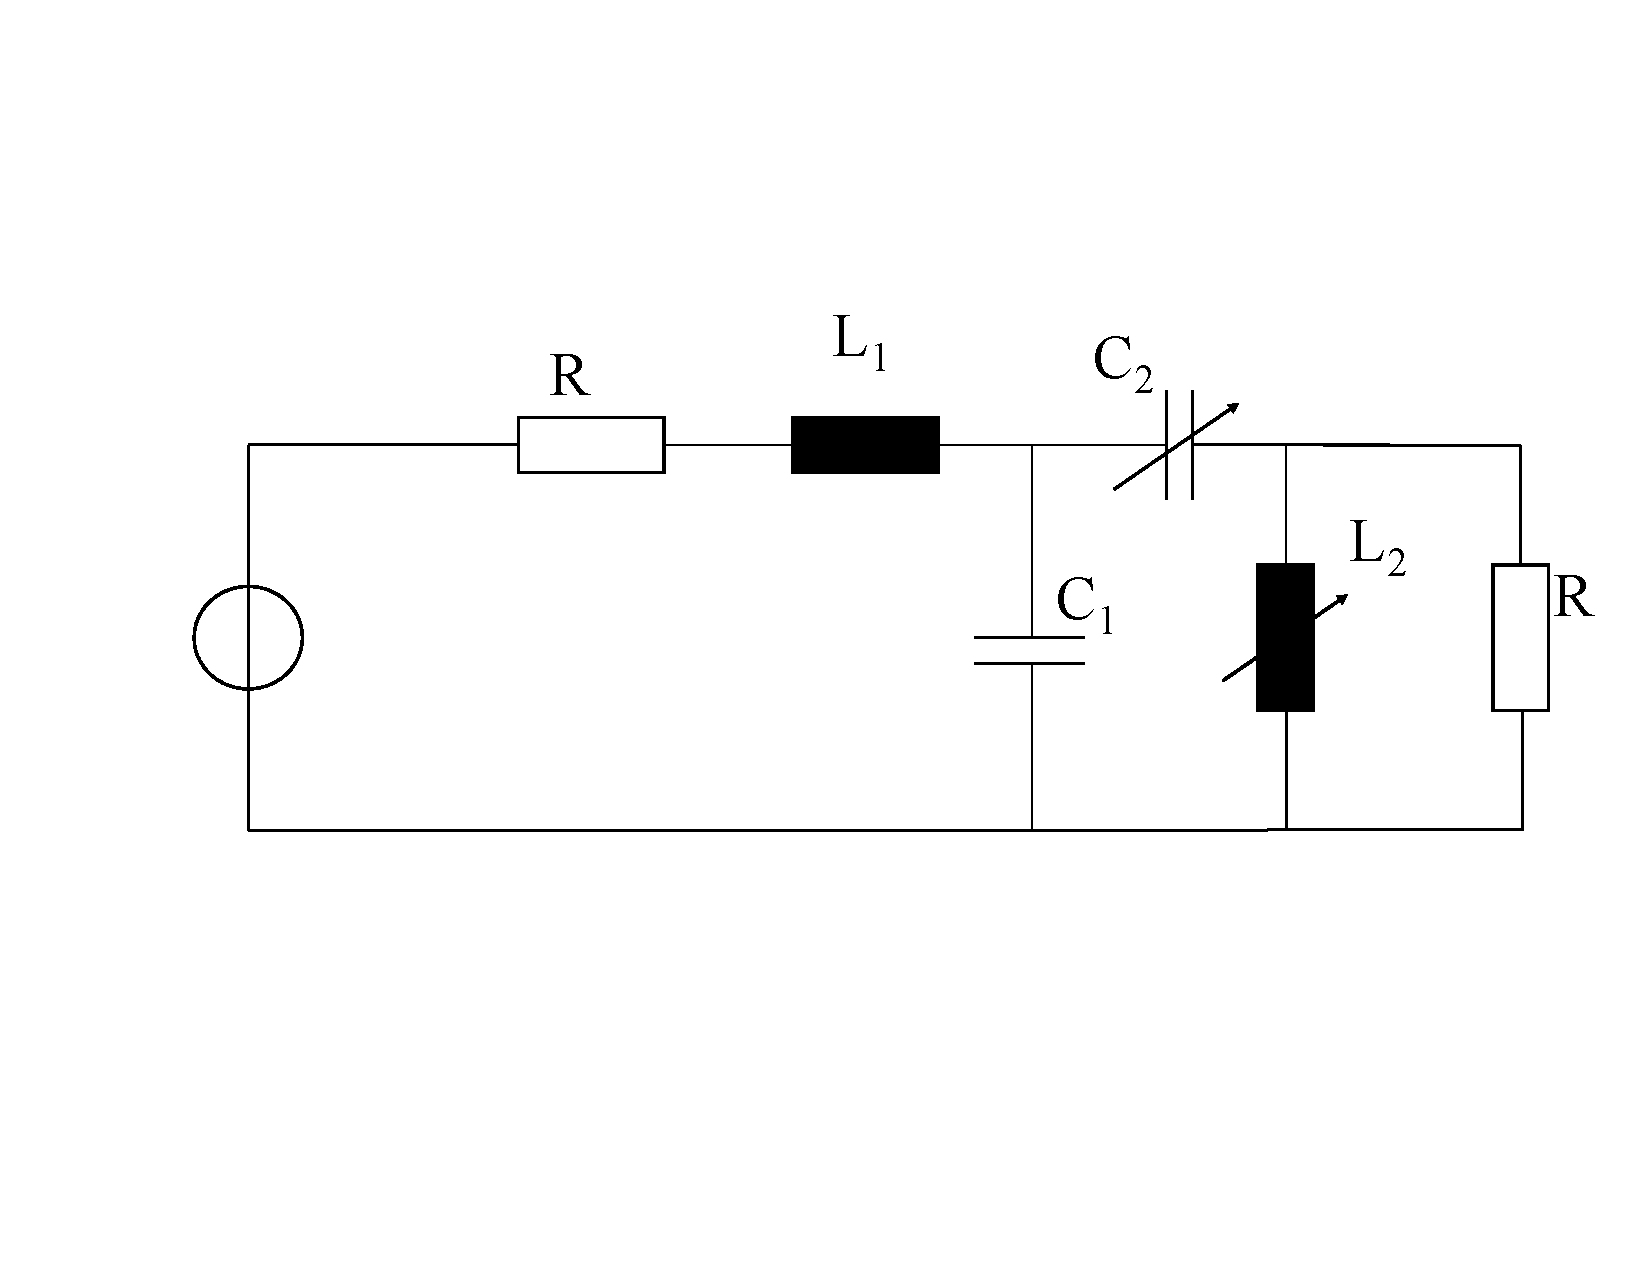
\includegraphics[scale=0.5, trim =1cm 7cm 1cm 5cm,clip ]{linear_filter.pdf}
	\caption{Linear Filter, fixed parameters}
	\label{linearfilter} 
\end{figure}
\subsection{Discrete Filter}
\begin{figure}[H]
	\centering
	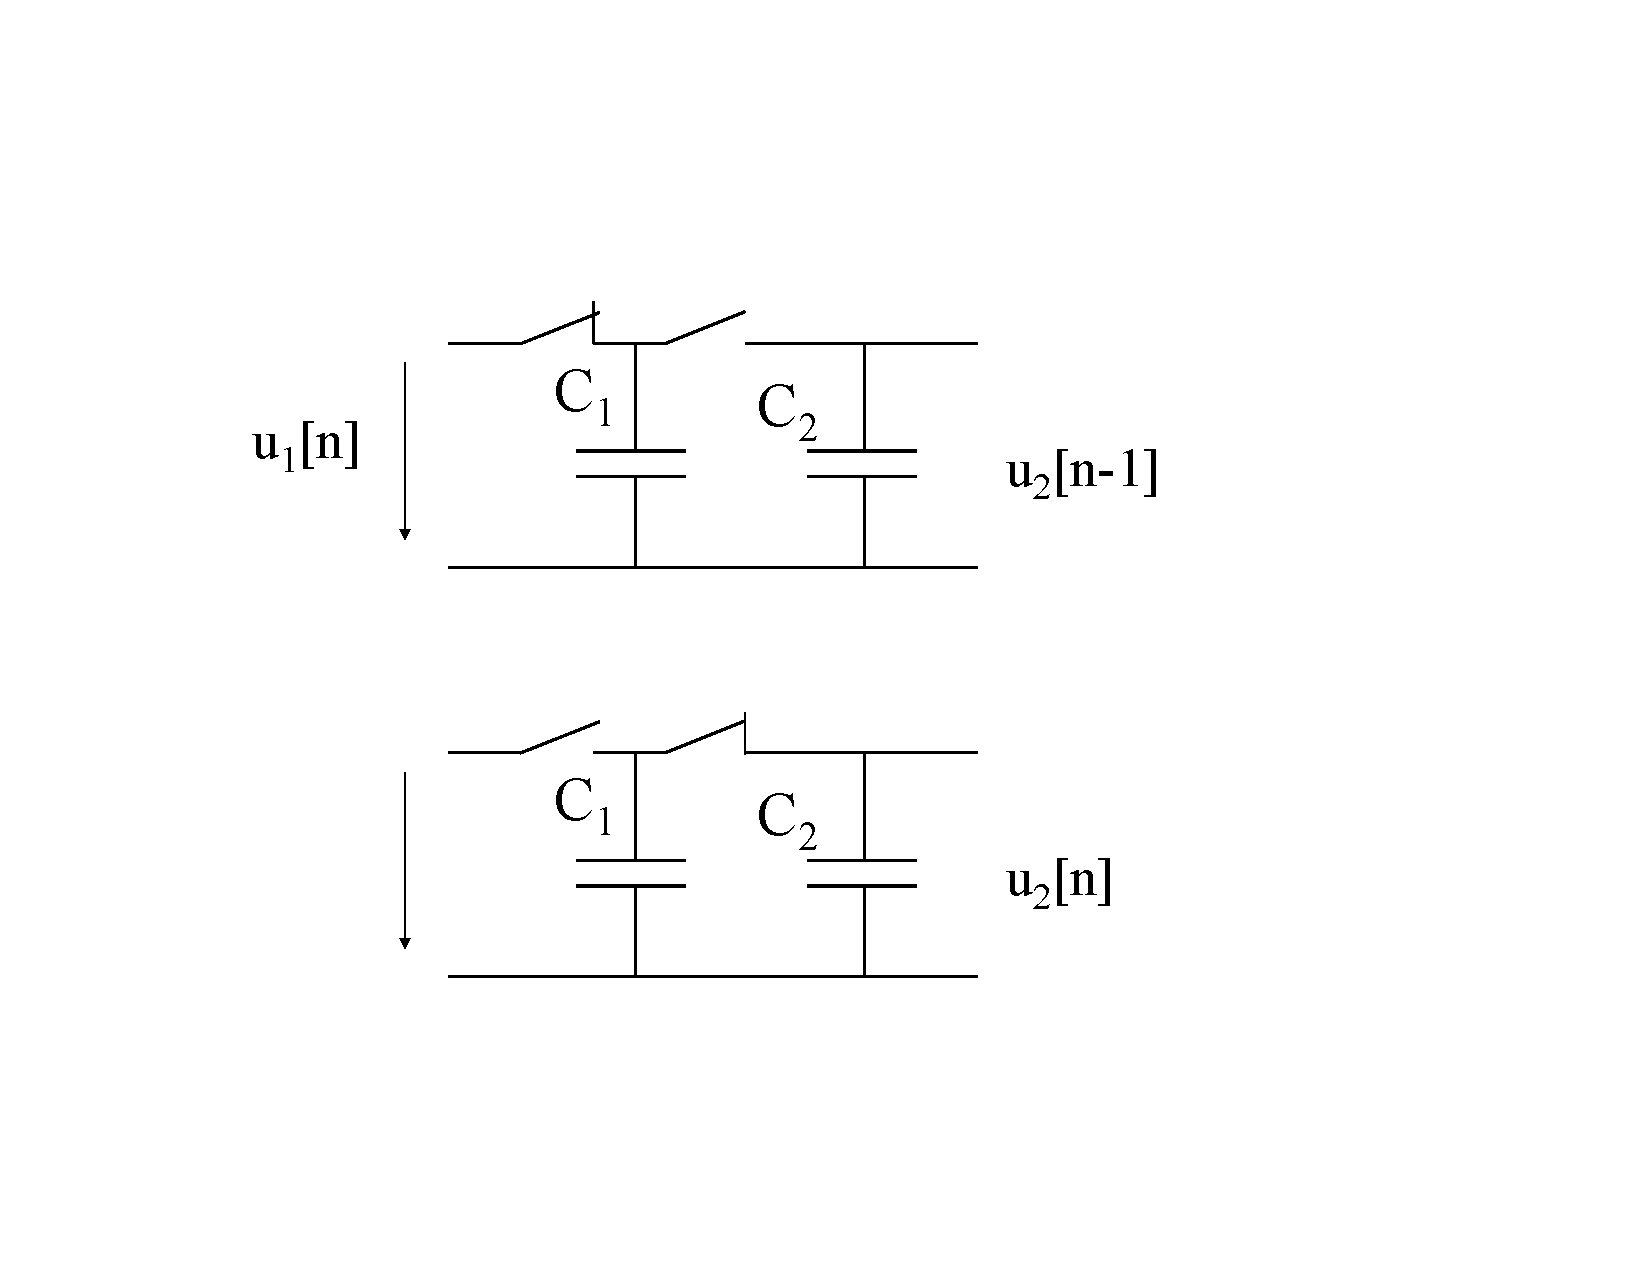
\includegraphics[scale=0.5, trim =3cm 5cm 6cm 5cm,clip ]{discrete_filter.pdf}
	\caption{One open, one closed, discrete time filter}
	\label{discretefilter} 
\end{figure}
\subsubsection{IIR-Filter}
Infinite impulse response (IIR) is a property applying to many linear time-invariant systems. Common examples of linear time-invariant systems are most electronic and digital filters. Systems with this property are known as IIR systems or IIR filters, and are distinguished by having an impulse response which does not become exactly zero past a certain point, but continues indefinitely. This is in contrast to a finite impulse response (FIR) in which the impulse response h(t) does become exactly zero at times $t > T$ for some finite T, thus being of finite duration.
The discrete filter in picture \ref{discretefilter} is defined by:\\ 
$C_1\cdot u_1[n] + C_2\cdot u_2[n-1] = (C_1+C_2 )u_2[n]$\\ 
$u_2[n]= \underbrace{\frac{C_2}{C_1+C_2}}_{a}\cdot u_2[n-1] + \underbrace{\frac{C_1}{C_1+C_2}}_{1-a}\cdot u_1[n]$\\
It's impulse response is given by table \ref{tab:prog_filter_Impulse_Resp}. As can be seen coefficient $a$ allows us to change the filter's impulse response and therefore to program the filter. Figure \ref{discreteeasy} shows a block diagram for such an easy, programmable discrete filter. From this block diagram it can be seen immediately that this filter is an IIR-Filter and can therefor be unstable.
\begin{figure}[H]
	\centering
	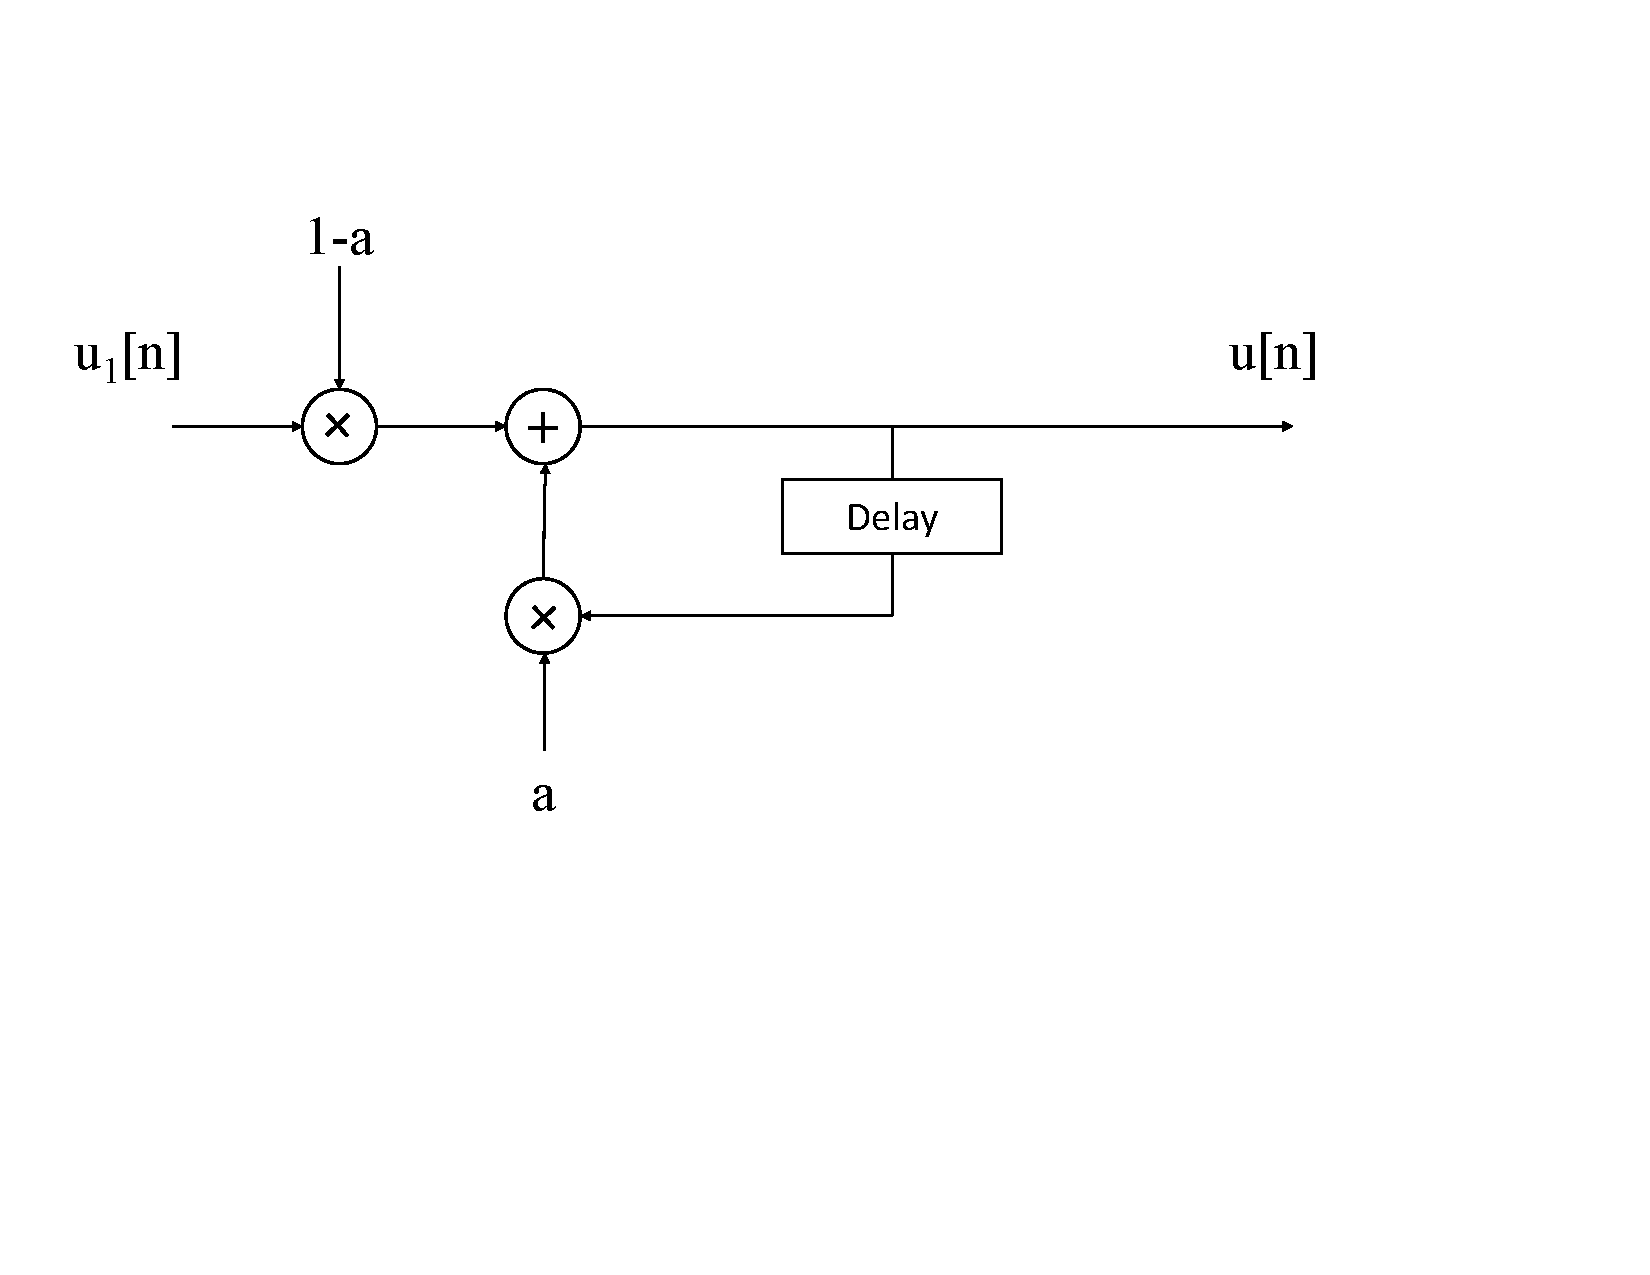
\includegraphics[scale=0.5, trim=1cm 7cm 3cm 2cm,clip]{discrete_easy.pdf}
	\caption{Discrete, easy to program filter}
	\label{discreteeasy} 
\end{figure}

\begin{table}
	\caption{discrete filter - Impulse Response }	
	\label{tab:prog_filter_Impulse_Resp}
	\centering
\begin{tabular}[H]{|c|cccccc|}
\hline
	n & $\leq$ 0 & 0 &1 &2 & ... &k\\
	\hline
	$u_1[n]$& 0 & 1 & 0 & 0 & ... &0\\
	$u_2[n]$& 0 & $1-a$ & $a(1-a)$&$ a^2(1a) $& ... & $a^k (1-a)$\\
	\hline
\end{tabular}
\end{table}

\textbf{Caution!} Proof of stability required! \\ $|a| \geq 1 \rightarrow $ instable \pfeil $|a| \leq 1 \rightarrow$ stable.
\begin{figure}[H]
	\centering
	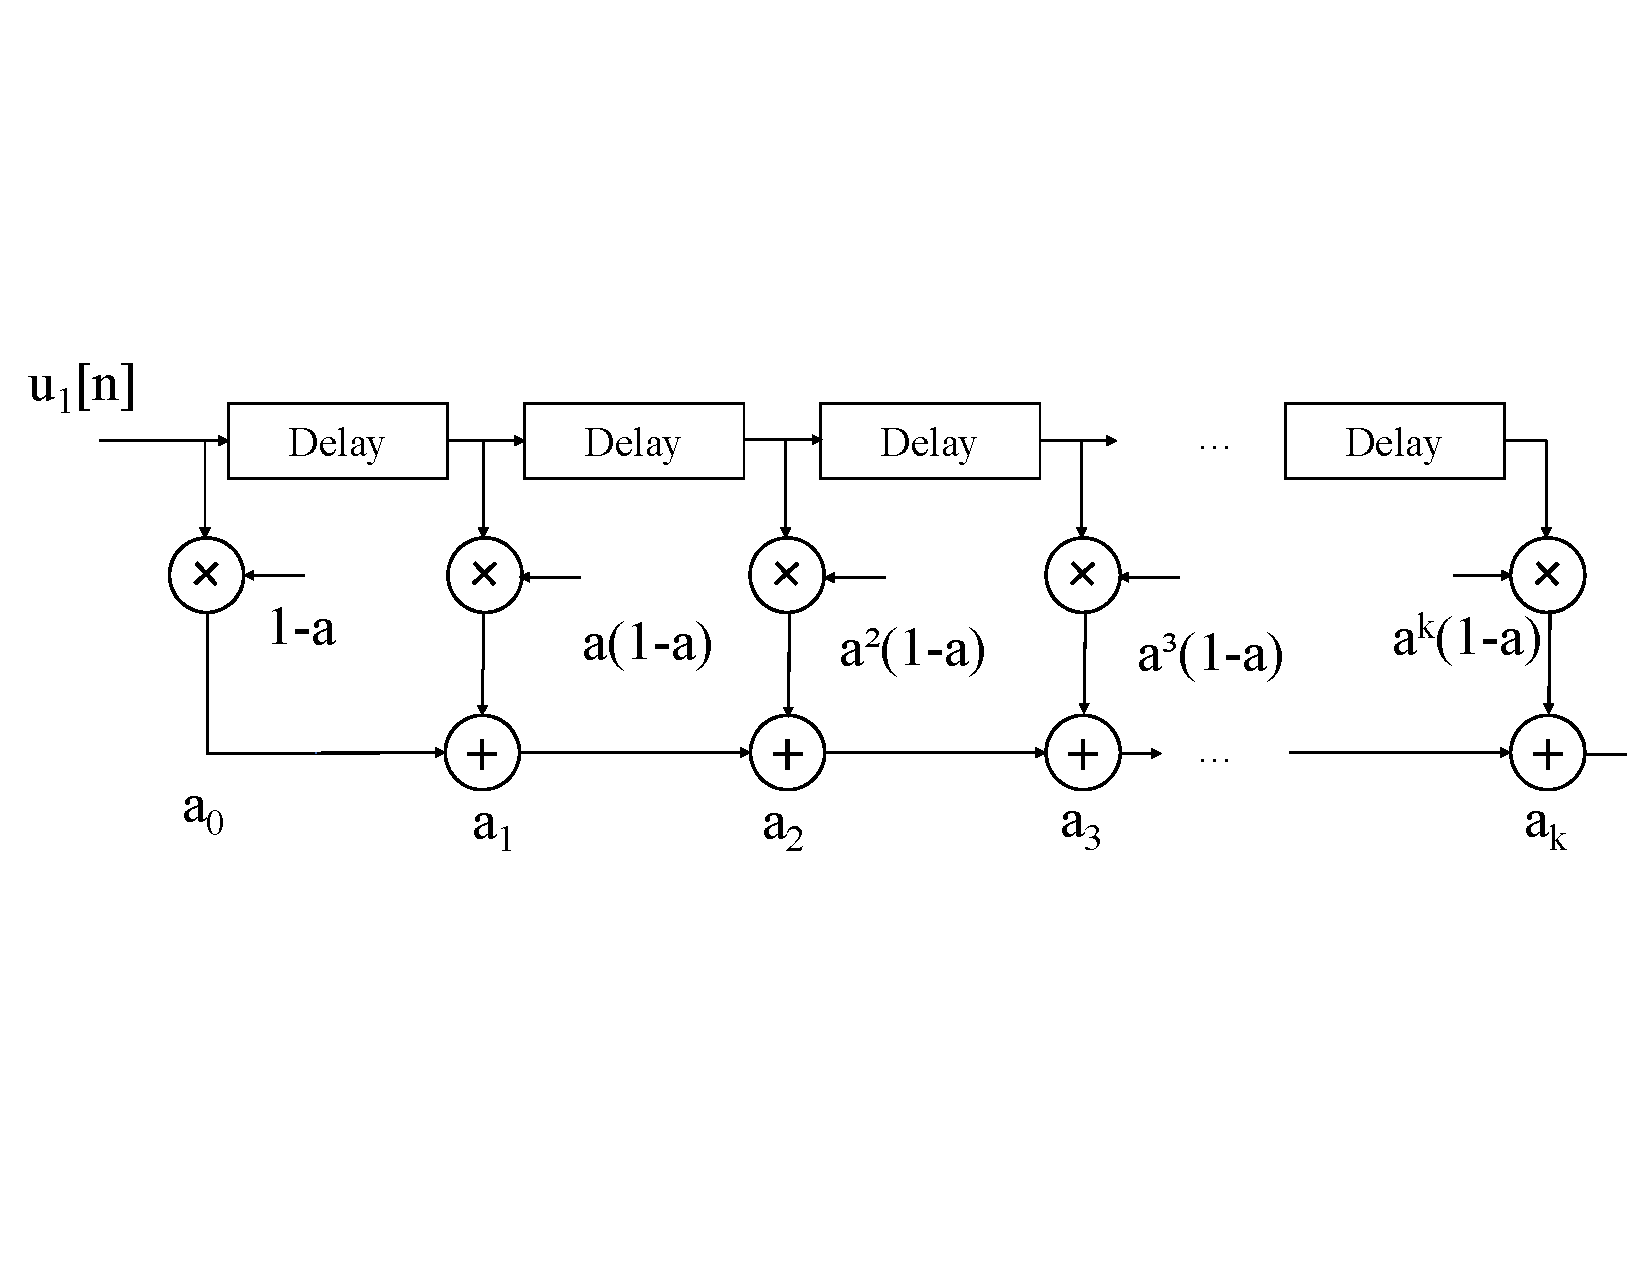
\includegraphics[scale=0.5, trim=0cm 5cm 0cm 5cm,clip]{delay_filter.pdf}
	\caption{Linear adaptive filter (tapped delay line)}
	\label{delayfilter} 
\end{figure}

\subsubsection{FIR-Filter}
To overcome the stability problems an FIR-filter can be used instead. FIR-Filters are always stable.
Suitable for adaptive filters but it's an approximation \pfeil finite \\
Structure: tapped delay line \\
linear: neither delay only coefficient are dependent in input signal. $\rightarrow$ linear adaptive filter, see picture \ref{delayfilter}.\\ \\

\textbf{Delays of 1 clock cycle:}\\
$D\cdot x[n] = x[n-1]$\\ \\
\textbf{Delay of 2 clock cycles:}\\
$\underbrace{DD}_{D^2}\cdot x[n] = D \cdot x[n-1] = x[n-2]= D^2\cdot x[n] $\\ \\

\textbf{Fractional delay:}\\
$F \cdot x(n) = x(n-\frac{1}{2})$\\
$FF \cdot x(n) = F \cdot x(n-\frac{1}{2}) = x[n-1] = D \cdot x[n]$\\
$F^2 = FF  	\equiv D ; F= \sqrt{D} = D^{\frac{1}{2}}$\\
$D^{\frac{1}{2}} \cdot D^{\frac{1}{2}} = D^{\frac{1}{2}+\frac{1}{2}} = D' =D$ \\
Developed using a Taylor series: $D^{\frac{1}{2}} \approx  1+\frac{1}{2}(D-1)+ \frac{1}{8}(D-1)^2 = \frac{3}{8}+\frac{3}{4}\cdot D + \frac{1}{8} D^2$\\
The filter in graphic \ref{delayfilter1_2} shows the shifting of the signal by $\frac{1}{2}$.
\begin{figure}[H]
	\centering
	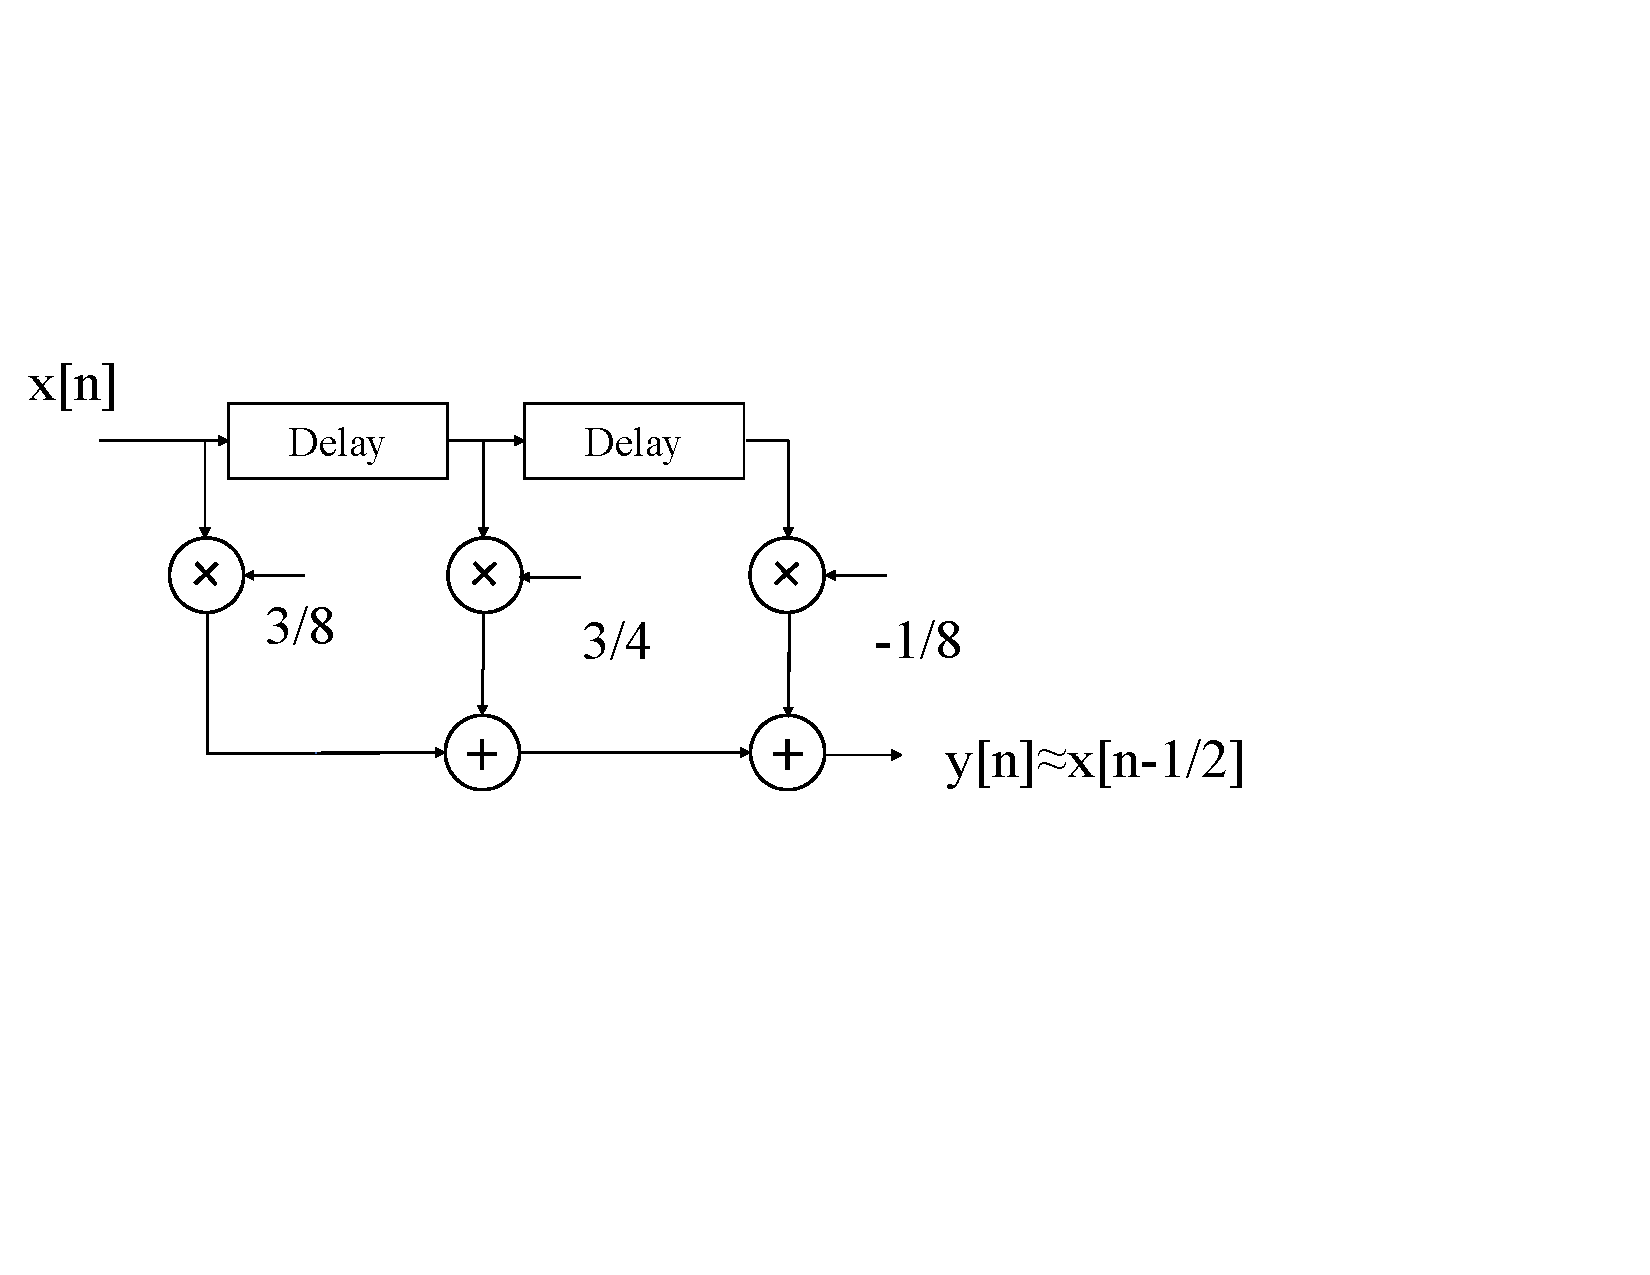
\includegraphics[scale=0.5, trim=0cm 8cm 0cm 6cm, clip]{delay_1_2.pdf}
	\caption{Used for synchronization of receiver and transmitter}
	\label{delayfilter1_2} 
\end{figure}

A fractional delay $y[n] \approx u[n-a] $ for $0 \leq a \leq 1$ \\
$y[n] = a_0 \cdot u[n] + a_1 \cdot u[n-1] + a_2 \cdot u[n-2] $ with $ a_0 = \frac{1}{2} (a^2 + 3a + 2)$ and $a_1 = (2-a)a$ and $a_2= \frac{1}{2} (a-1) a $\\

\begin{figure}[H]
	\centering
	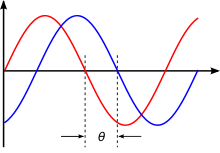
\includegraphics{phaseshift.png}
	\caption{Phase-shift for $\theta$}
	\label{phaseshift} 
\end{figure}

\textbf{Example:} $a=\frac{1}{2} \quad u[n]=sin(\frac{n}{2})$\\
A node is passing \[ S= \sum_{i=1}^2 |a_i|^2 = \frac{1}{2}a^4 - 6a^3 +\frac{5}{2} a^2 - 3a+1\] remains $\leqq 1$ only for $0\leq a\leq 2$. For $a < 0  $ or $a > 2$ it grows unboundenly.\\ This is relevant, since uncorrelated noise at the input leads to an output which mean square is proportional to S. Thus, $a < 2$ or $a < 0$ are possible, but with a (huge) noise penalty. The mean squared output noise is minimum for $a = 1-\frac{1}{\sqrt{2}} \approx 0,3$
\begin{figure}[H]
	\centering
	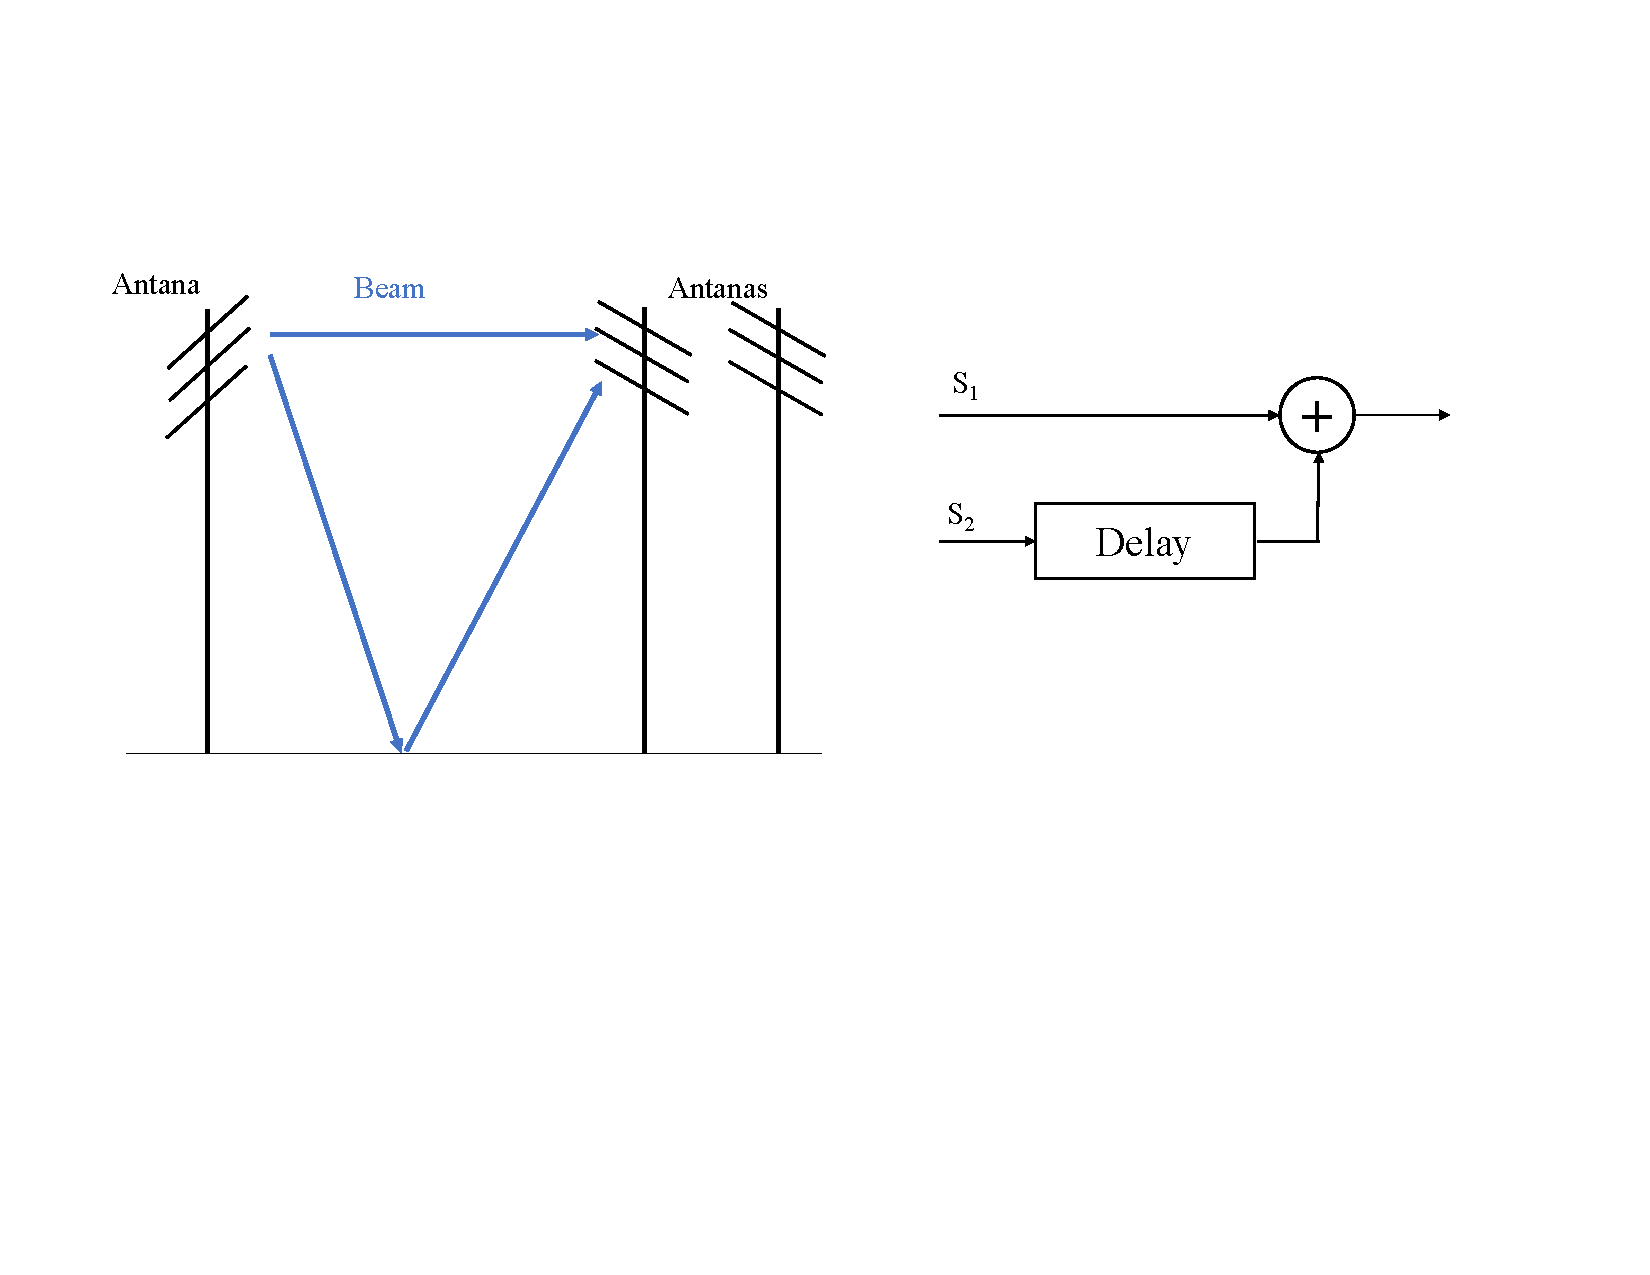
\includegraphics[scale=0.5, trim=1cm 8cm 1cm 4cm, clip]{antenna.pdf}
	\caption{2 signals, but delayed.}
	\label{delayedsignal} 
\end{figure}
The sketch in figure \ref{delayedsignal} shows a signal which travels trough two paths from the transmitter to the receiver. One signal is faster (has a shorter way) than the other. To be able to add the two signals the faster one has to be delayed and since the delay between the two signals is (usually) not an integer the fractional delay is needed here.\\
 \pfeil After delaying the faster one, they're only different in their amplitude and can be added. (Otherwise we get fading effects.)

\subsection{Principle Structure of an Adaptive Filter}


\begin{figure}[H]
	\centering
	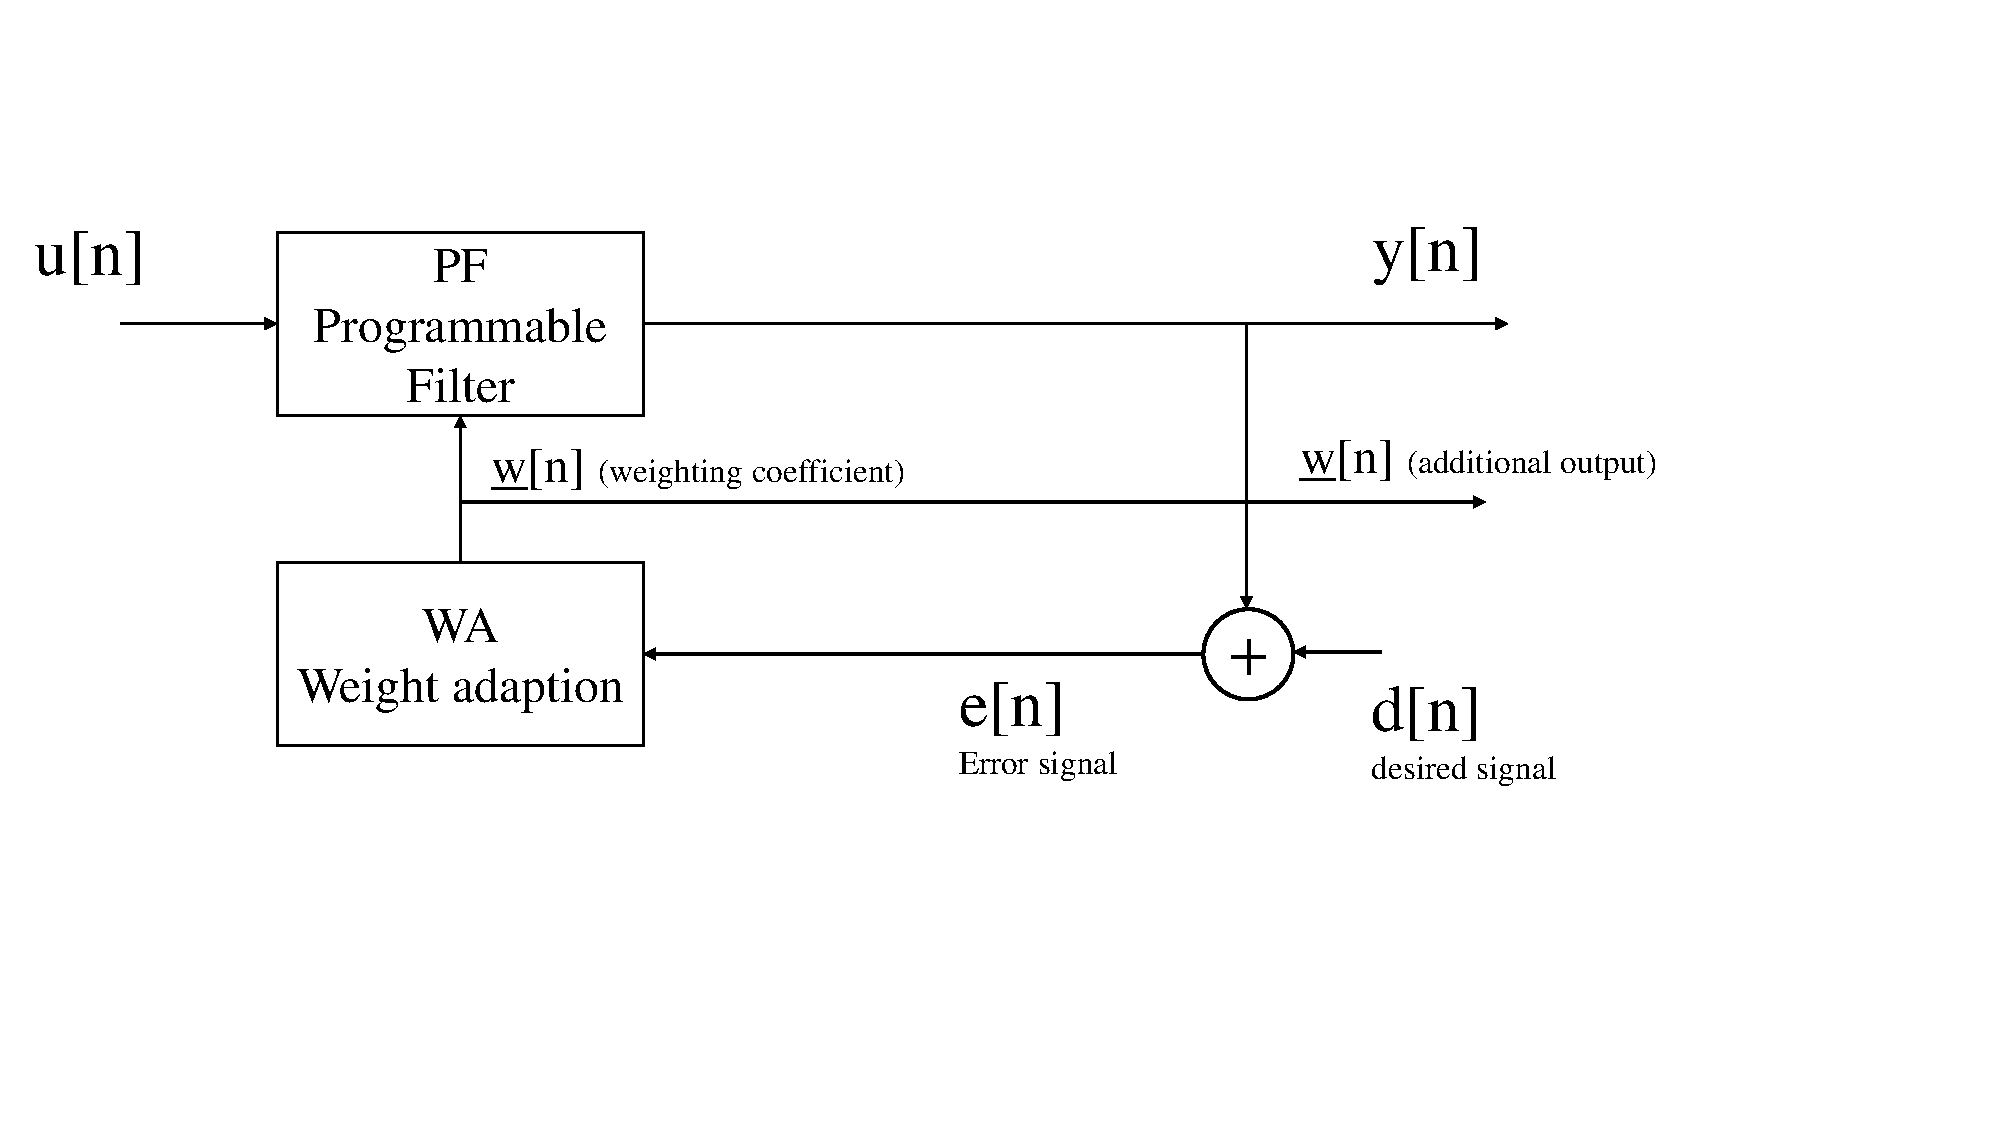
\includegraphics[scale=0.5, trim=0cm 5.5cm 0cm 3cm, clip]{adaptive_filter.pdf}
	\caption{Principle structure of an Adaptive Filter}
	\label{adaptive_filter} 
\end{figure}

$e[n] = 0 \pfeil \underline{w} [n+1] = \underline{w} [n]$
\subsubsection{The 4 Application Classes}
\textbf{System Identification}
	\begin{figure}[H]
		\centering
		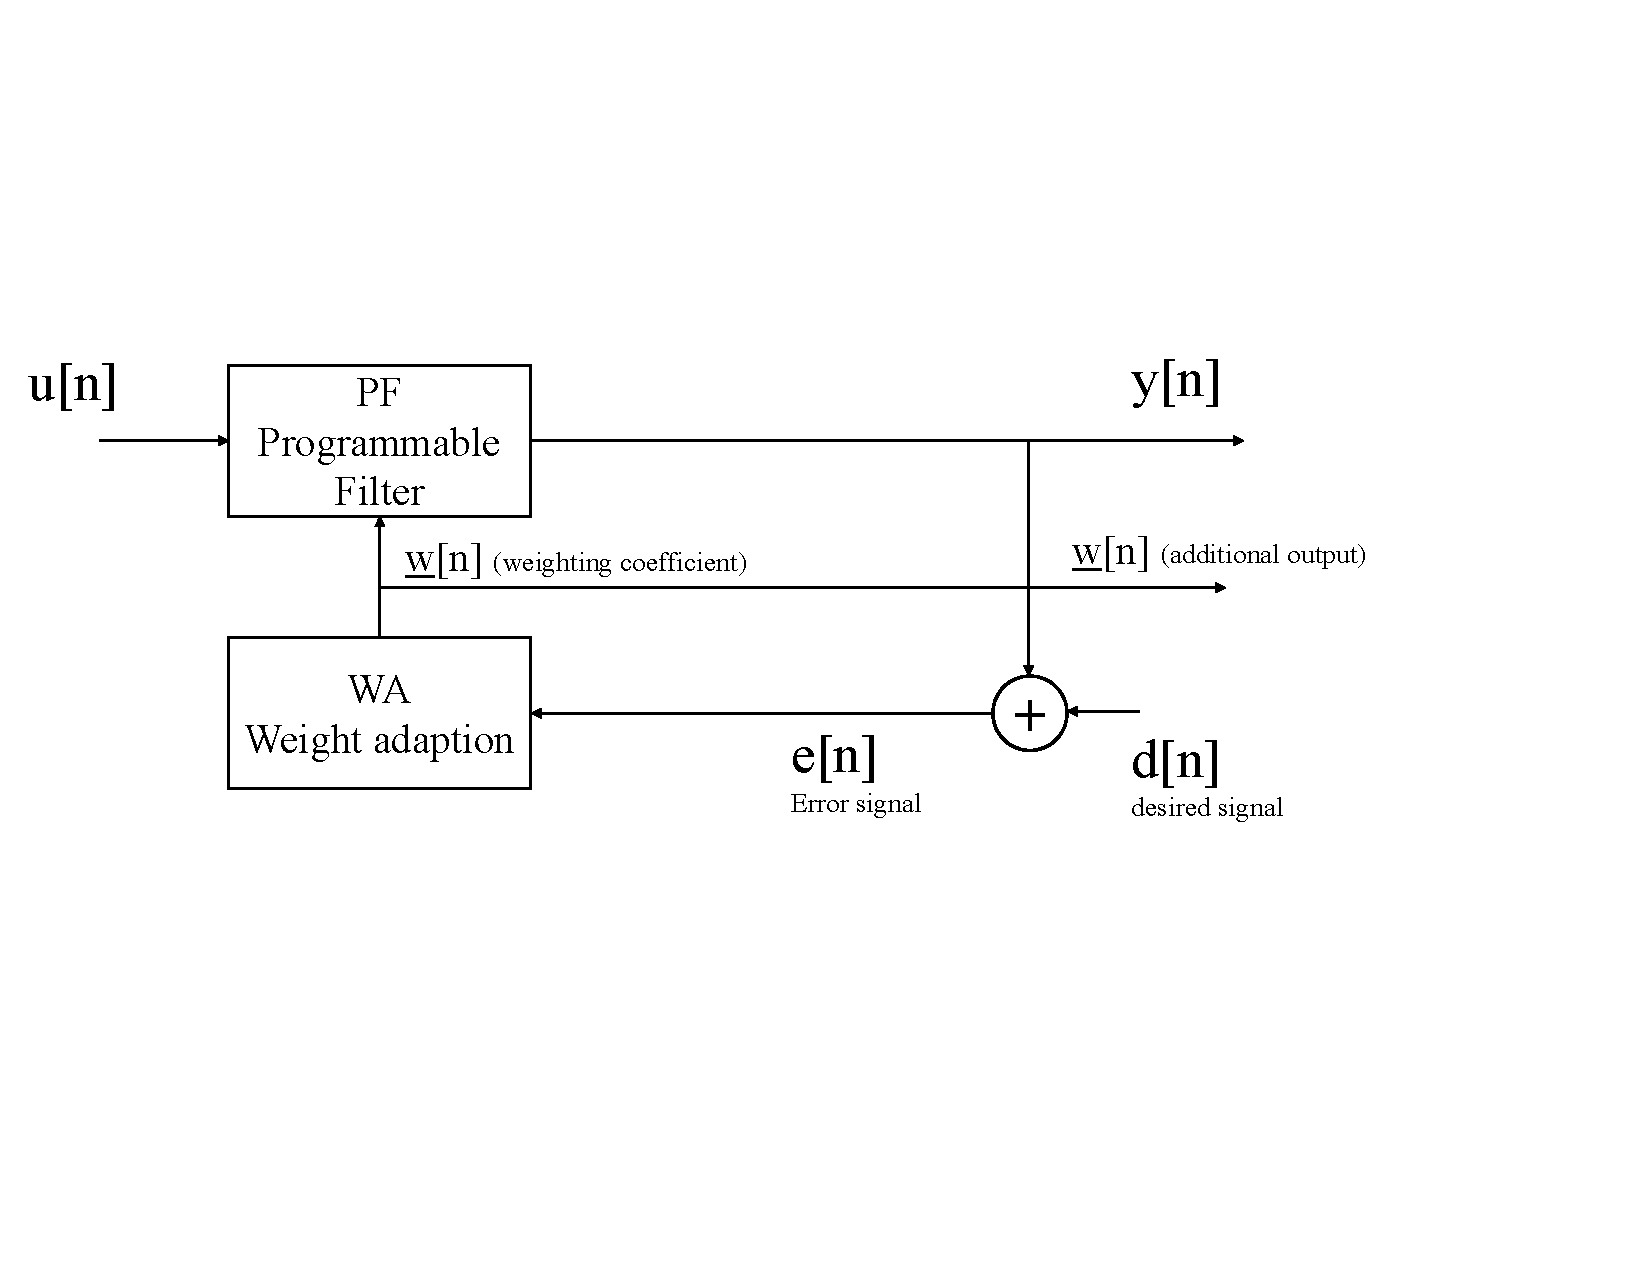
\includegraphics[scale=0.5, trim=0cm 5cm 0cm 5cm, clip]{system_identification.pdf}
		\caption{System identification}
		\label{system_identification} 
	\end{figure}

\textbf{Channel Estimation}
	\begin{figure}[H]
	\centering
	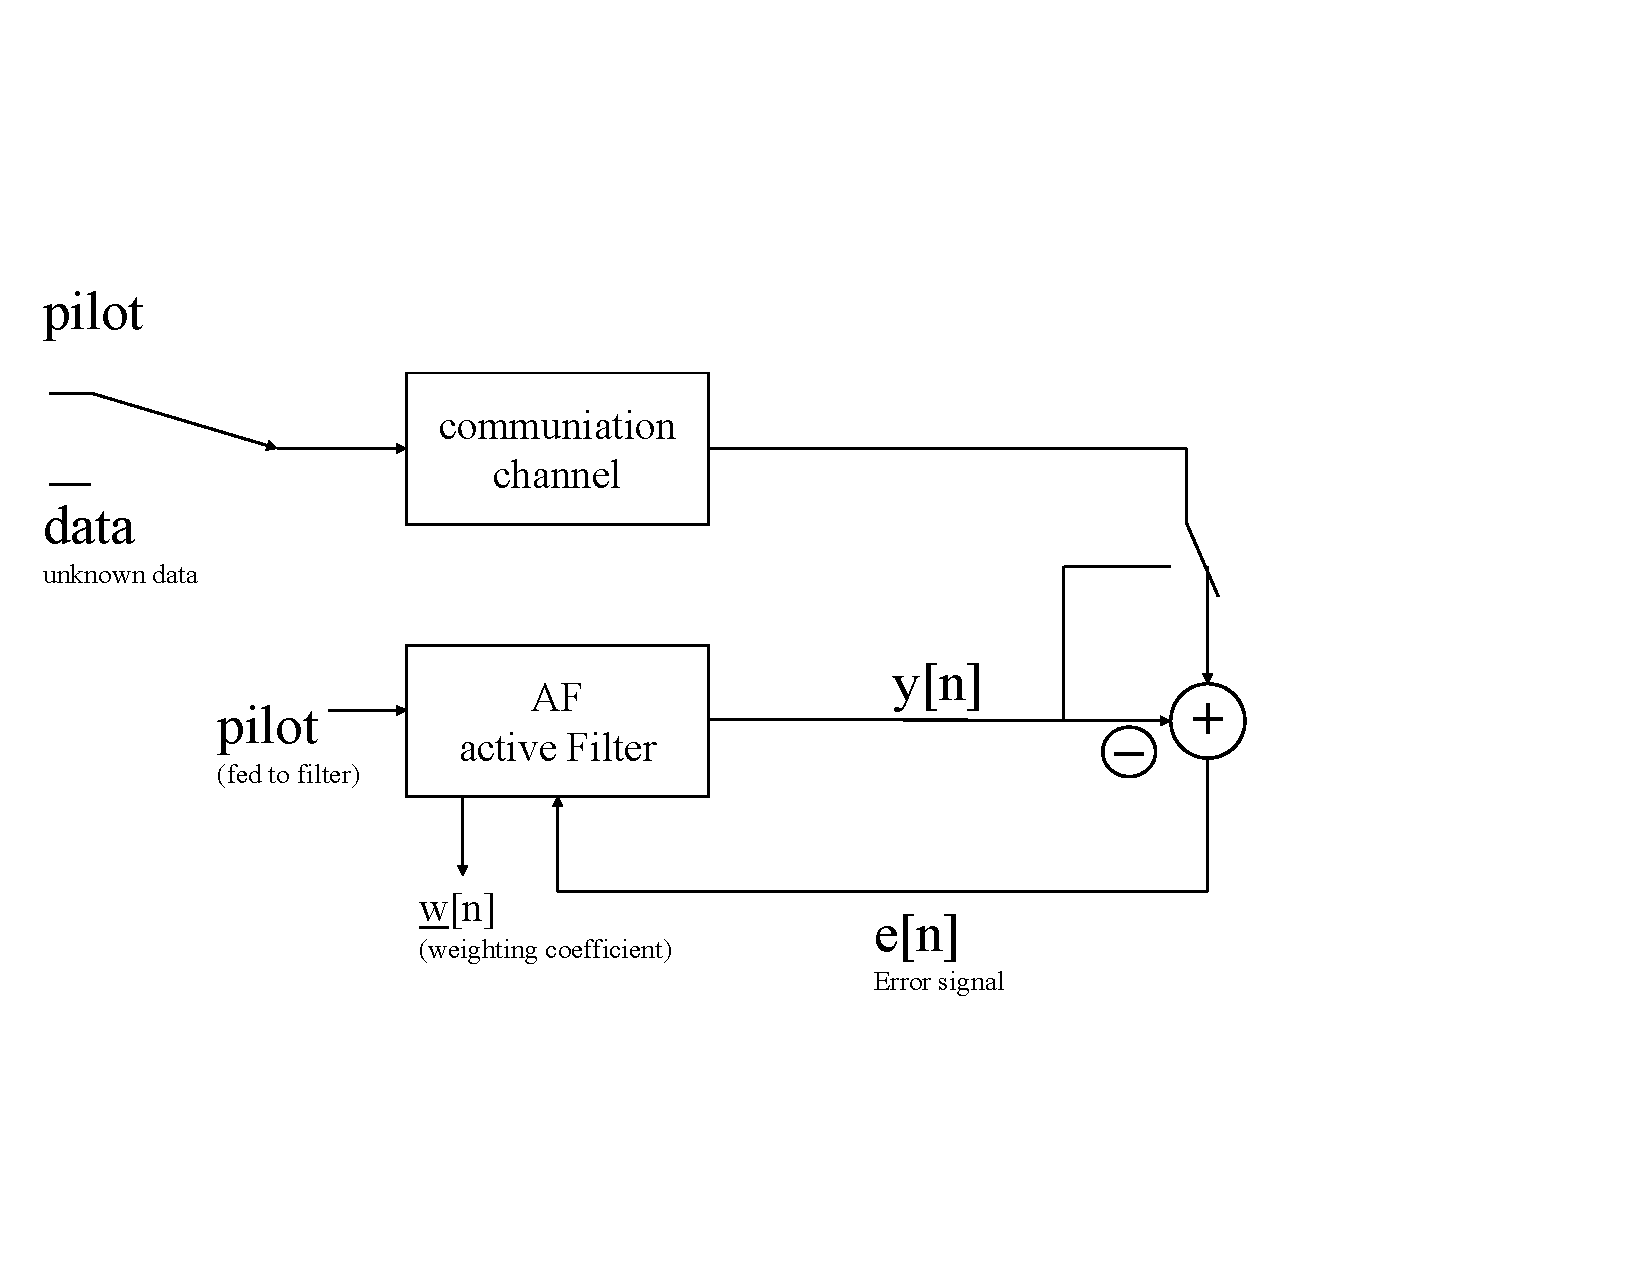
\includegraphics[scale=0.5, trim=0cm 4cm 0cm 5cm, clip]{channel_estimation.pdf}
	\caption{Channel Estimation}
	\label{channel_estimation} 
\end{figure}
The Pilot is a known data string. Either the transmitter and the receiver know the pilot. The data is unknown.

\textbf{Inverse Modelling}
	\begin{figure}[H]
	\centering
	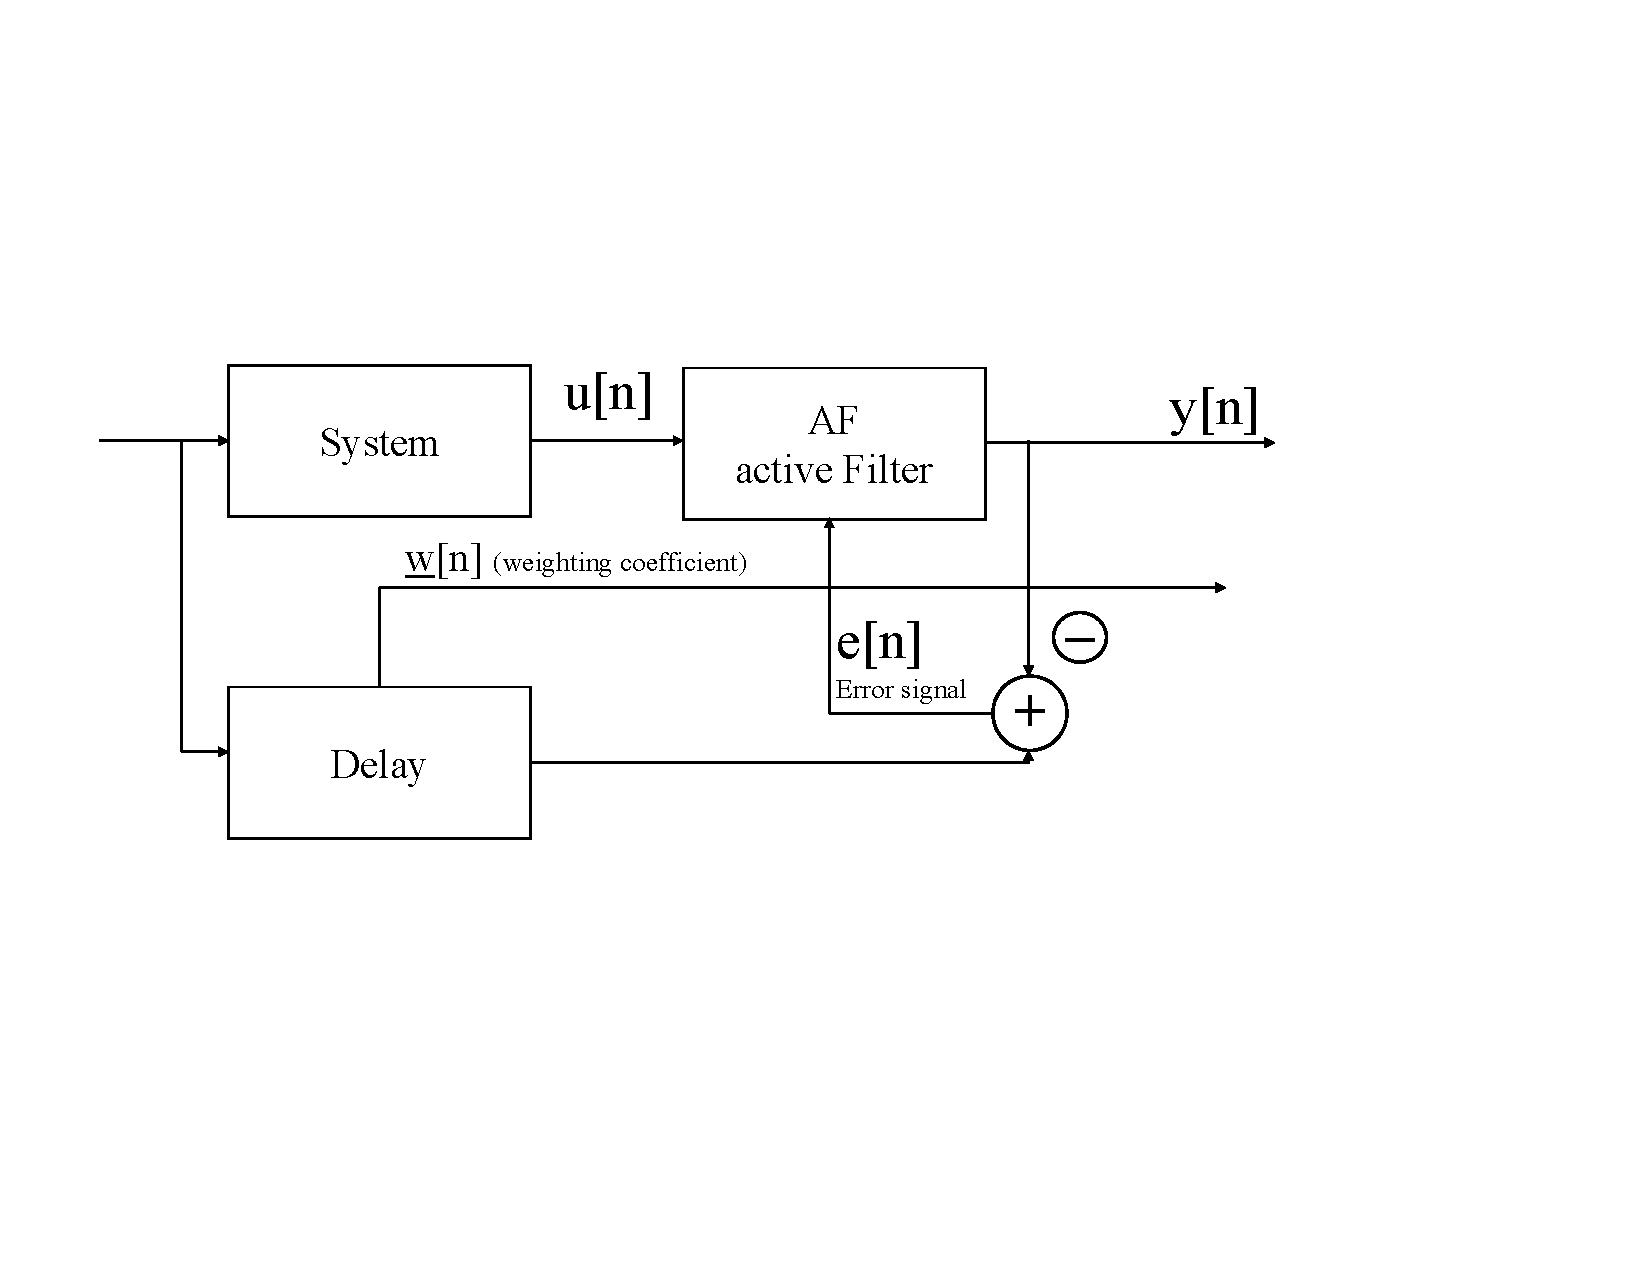
\includegraphics[scale=0.5, trim=0cm 7cm 0cm 5cm, clip]{inverse_modelling.pdf}
	\caption{Inverse Modelling}
	\label{inversemodelling} 
\end{figure}
Example to picture \ref{inversemodelling}: Channel equilization (interested in data, not the channel).\\
\textbf{Prediction}
	\begin{figure}[H]
	\centering
	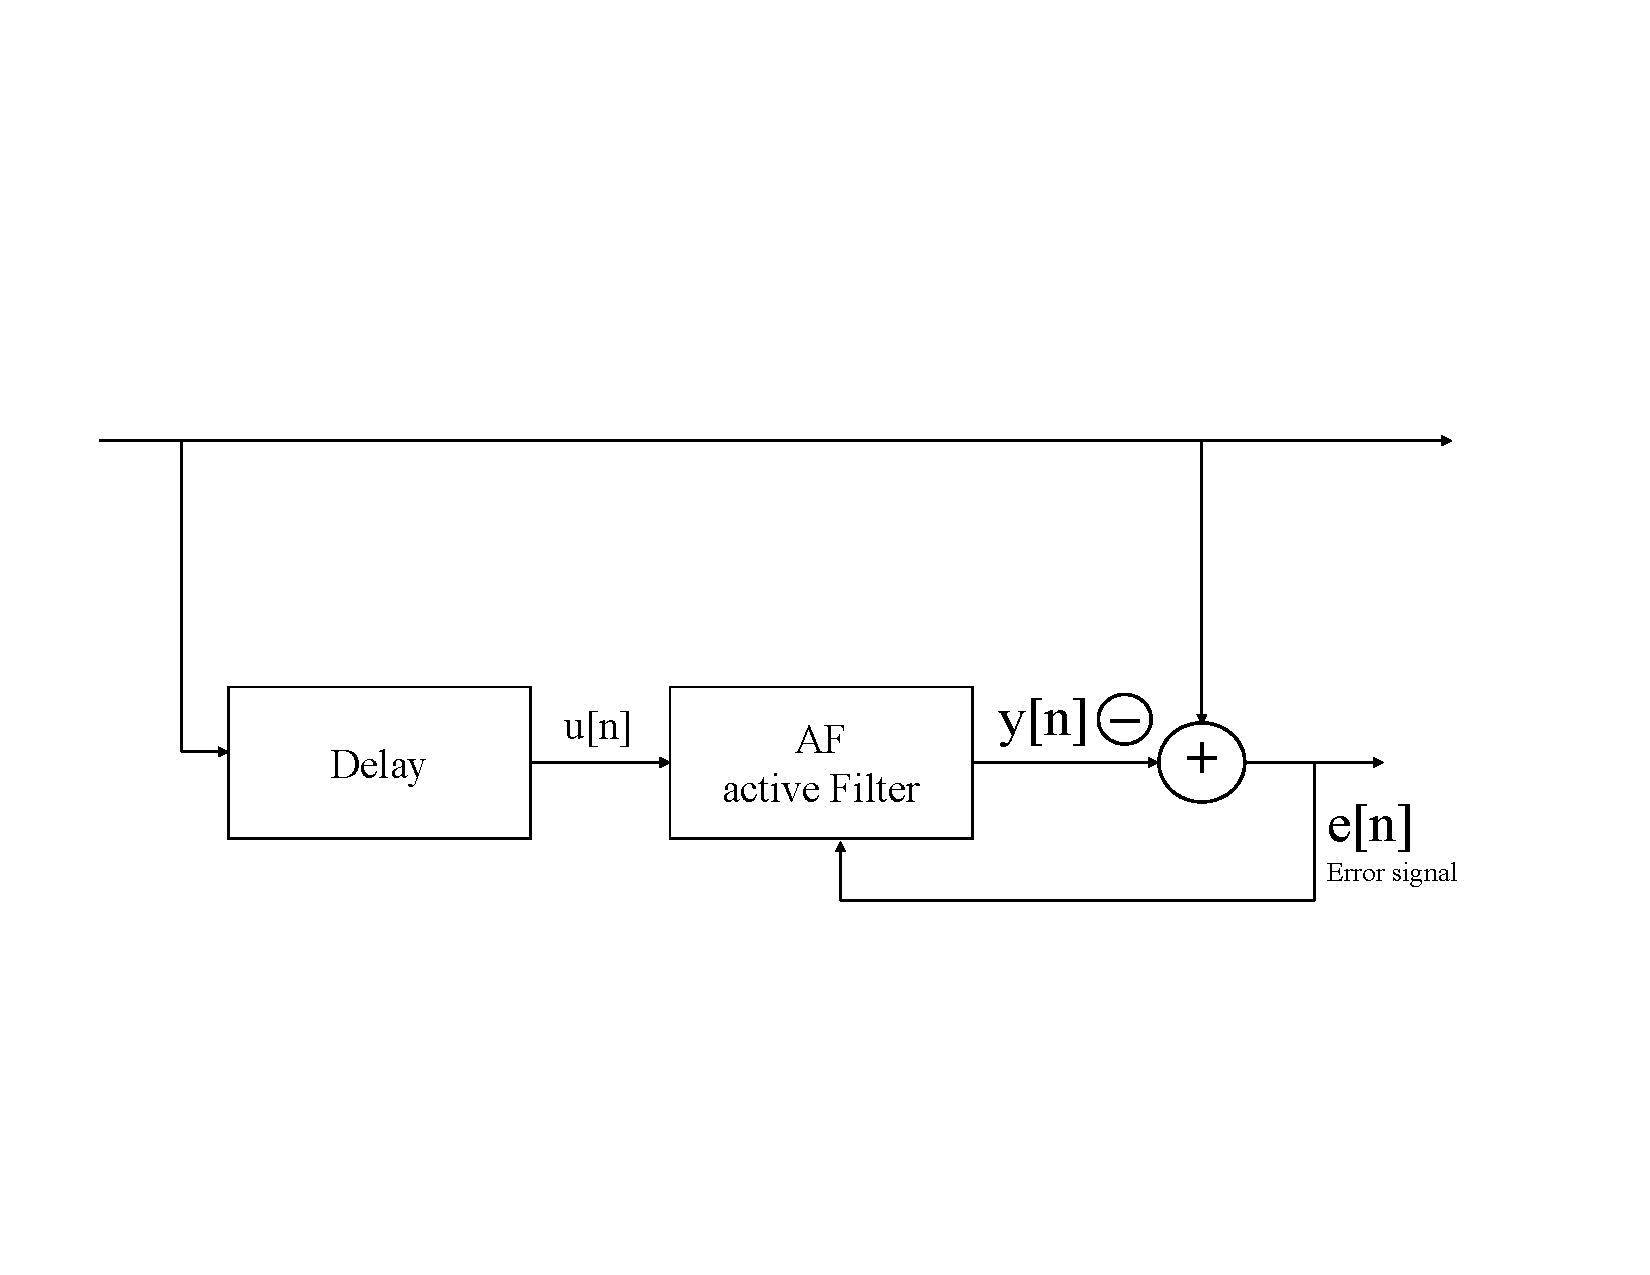
\includegraphics[scale=0.5, trim=0cm 4cm 0cm 5cm, clip]{prediction.pdf}
	\caption{Prediction}
	\label{prediction} 
\end{figure}
Notes to \ref{prediction}: Blind to future and present, but knows the past.. Trouble: if quantized e[n] won't work!\\
Therefore:\\
	\begin{figure}[H]
	\centering
	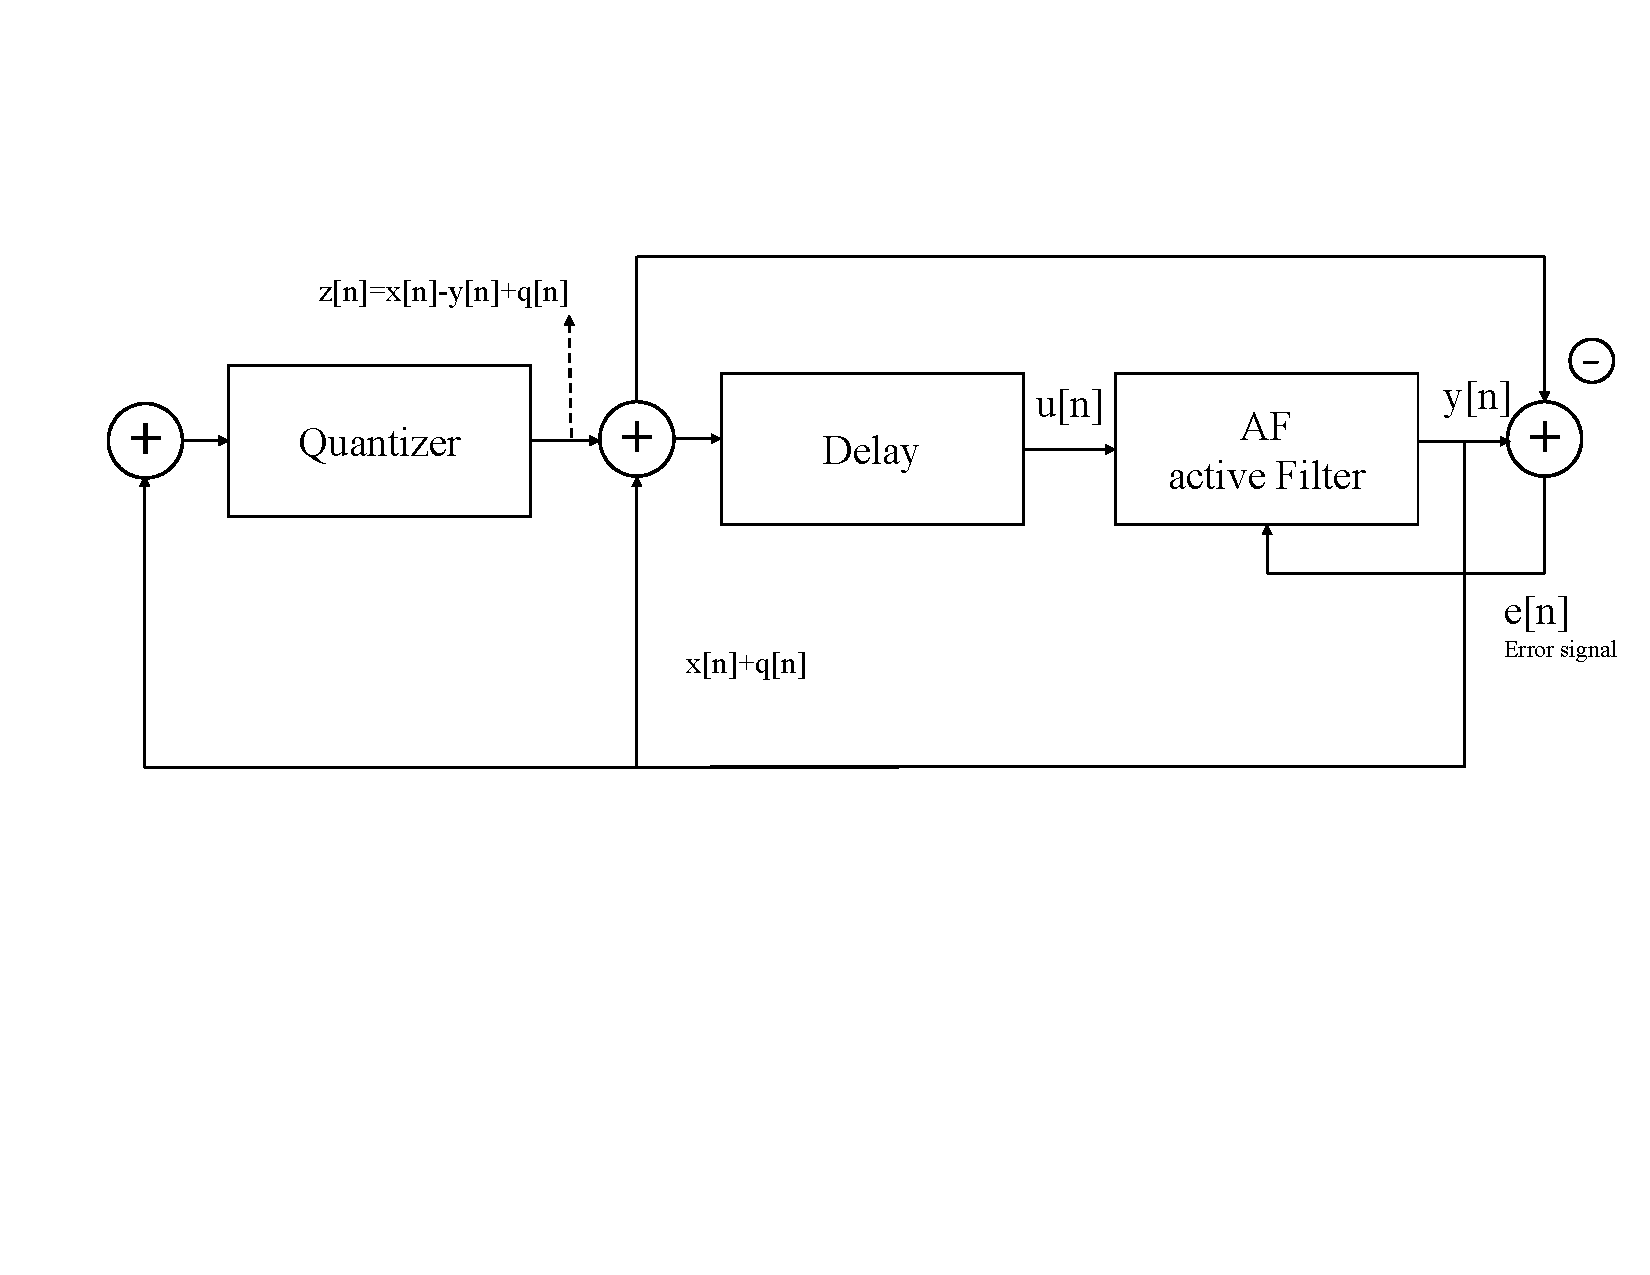
\includegraphics[scale=0.65, trim=0cm 7cm 0cm 3cm, clip]{compressor.pdf}
	\caption{Compressor}
	\label{compressor} 
\end{figure}
Predictive filter works well \pfeil if error is small\\
	\begin{figure}[H]
	\centering
	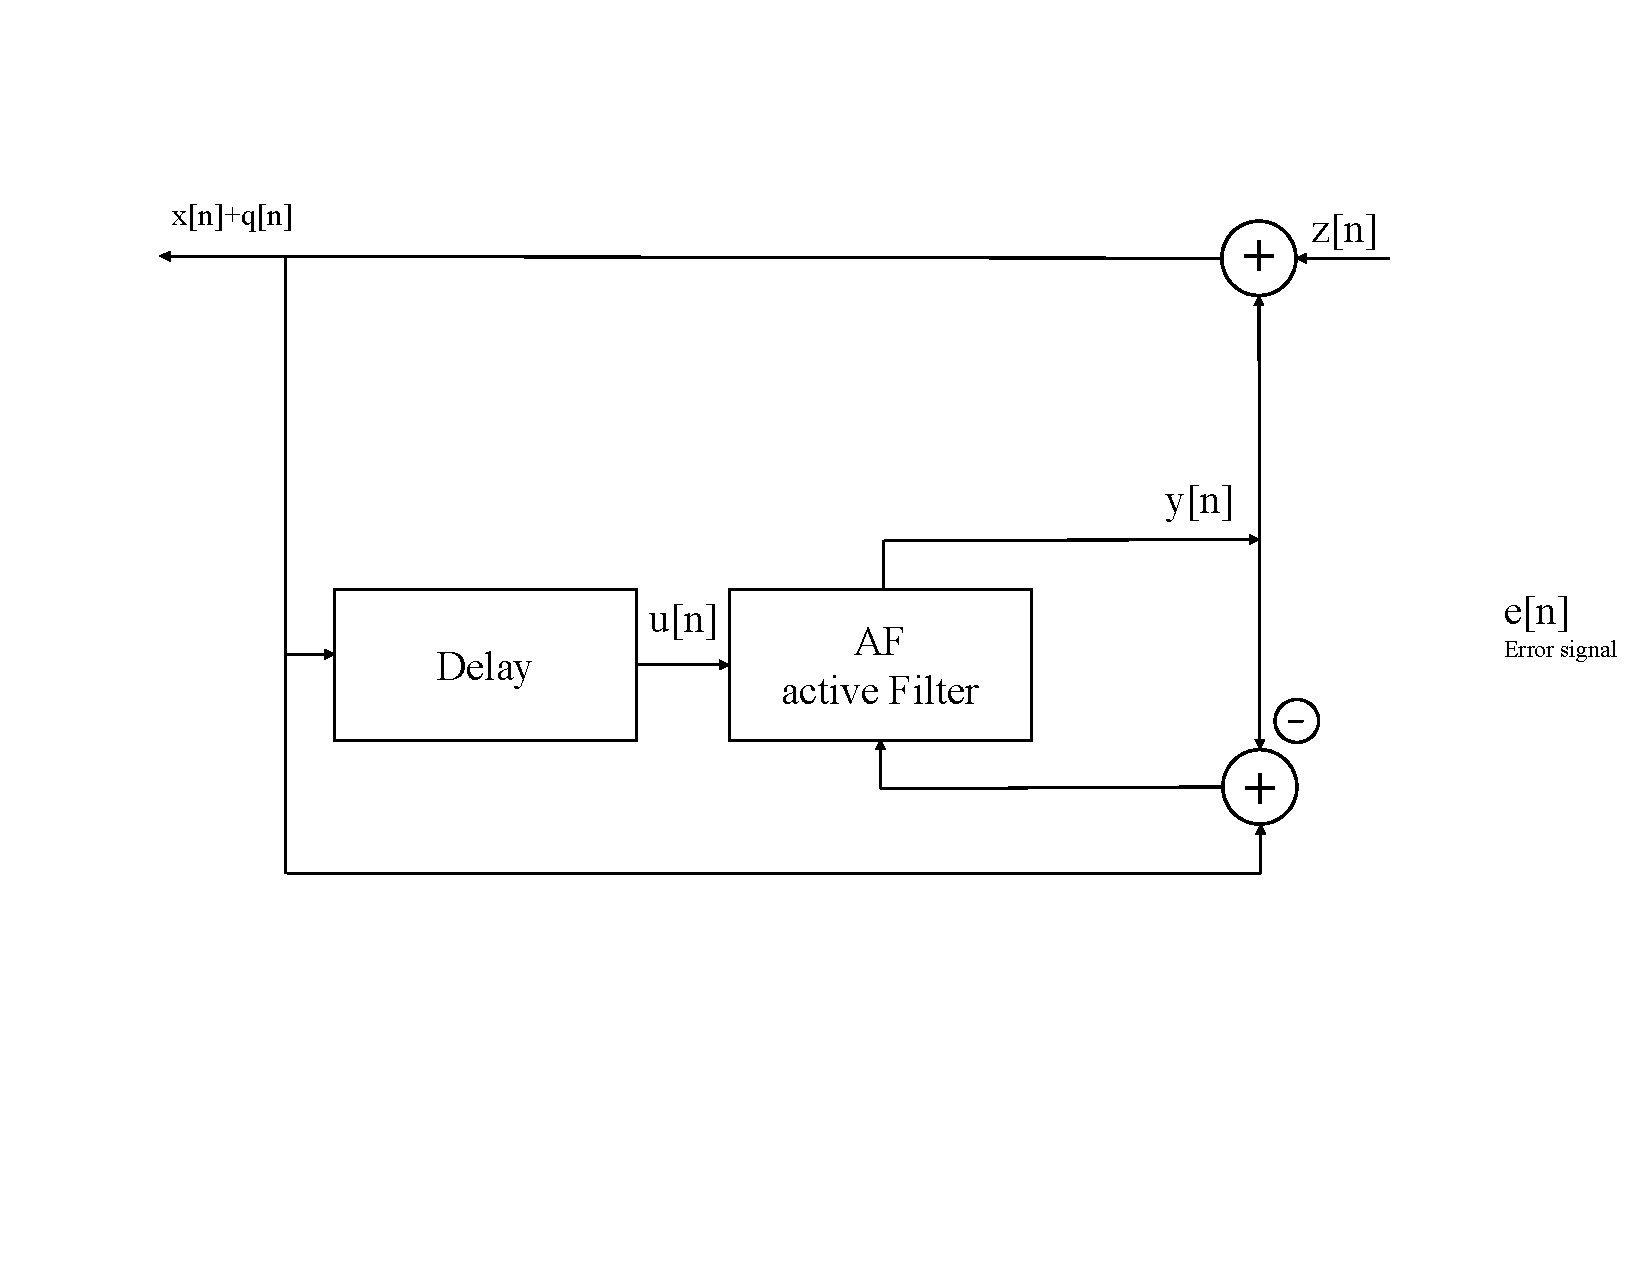
\includegraphics[scale=0.65, trim=0cm 5cm 0cm 2cm, clip]{decompressor.pdf}
	\caption{Decompressor}
	\label{decompressor} 
\end{figure}

\textbf{Interference Cancellation}
	\begin{figure}[H]
	\centering
	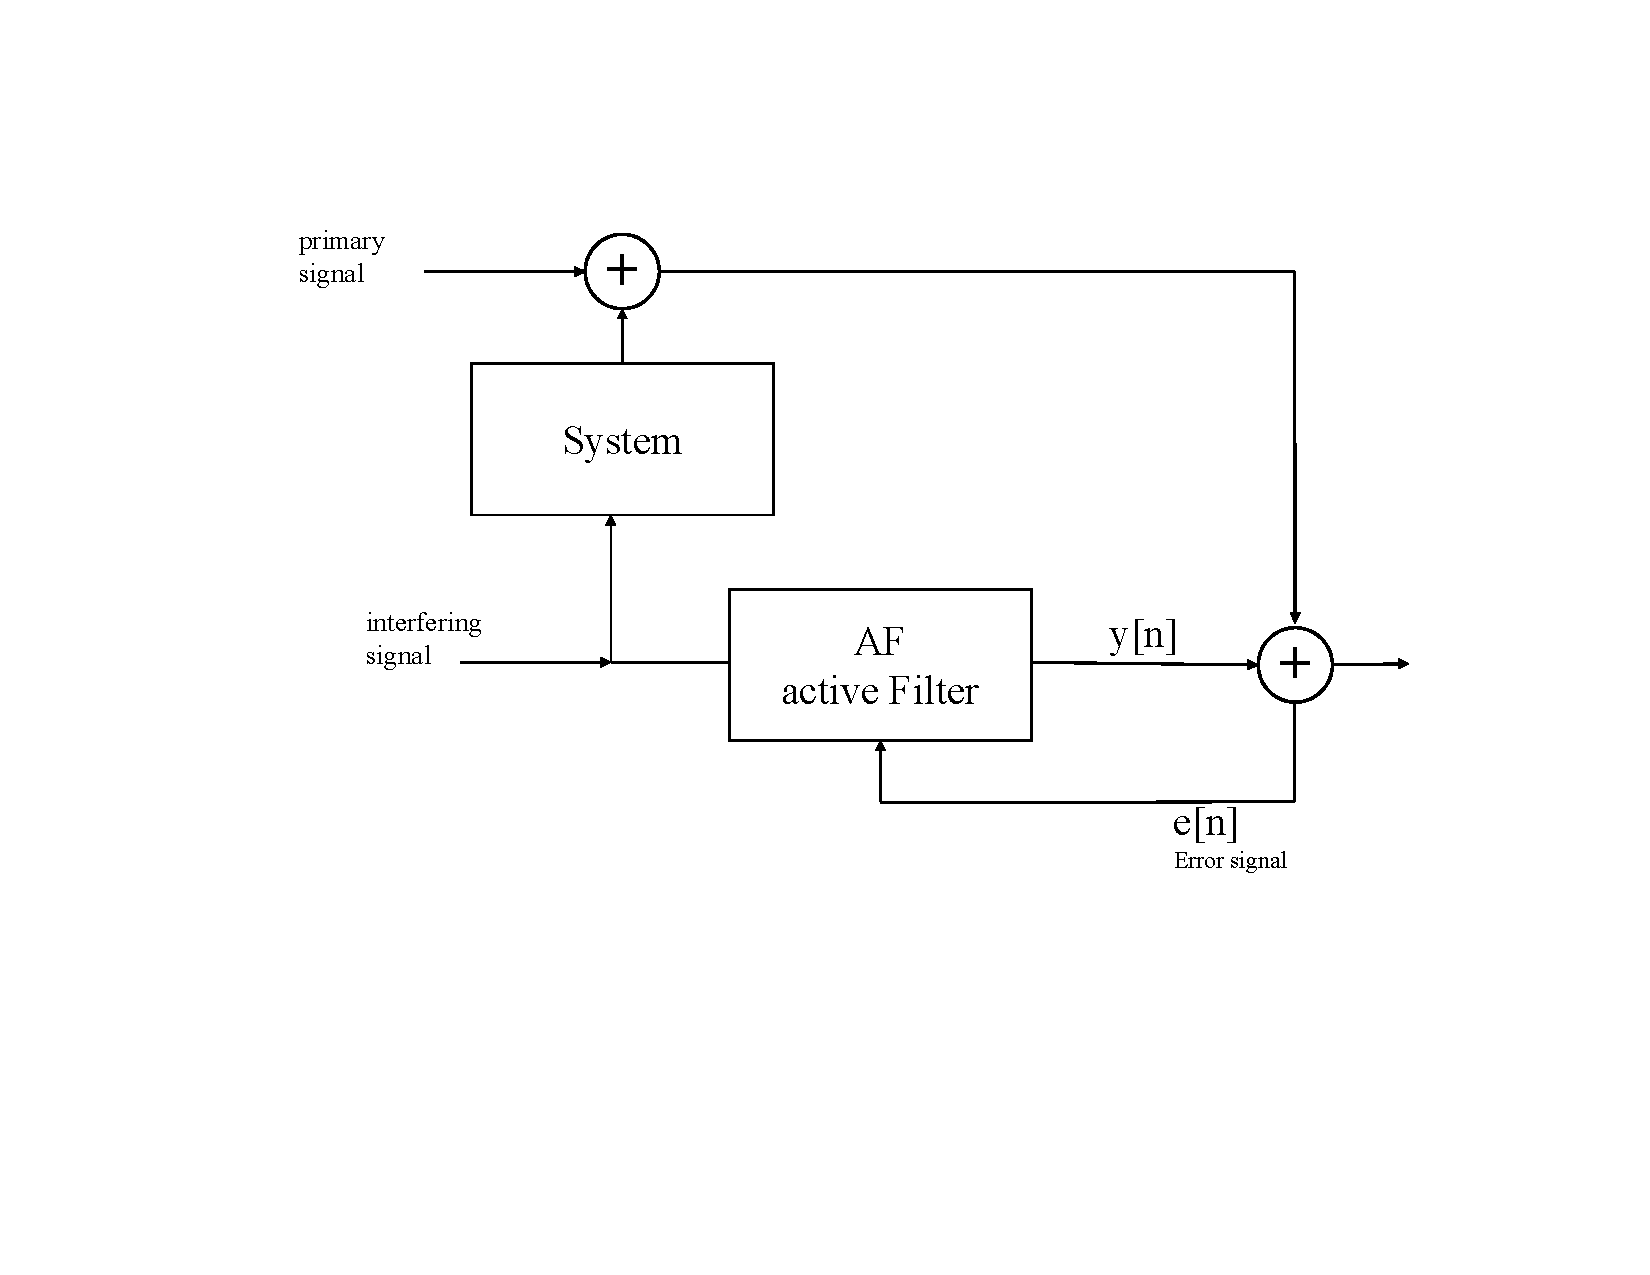
\includegraphics[scale=0.65, trim=0cm 6cm 0cm 3cm, clip]{interference_chanellation.pdf}
	\caption{Interference Cancellation}
	\label{interference1} 
\end{figure}
Assumption: The desired (primary) signal is statistically independent of the interfering signal.\\
For linear adaptive filters: uncorrelated is enough. 
\begin{figure}[H]
	\centering
	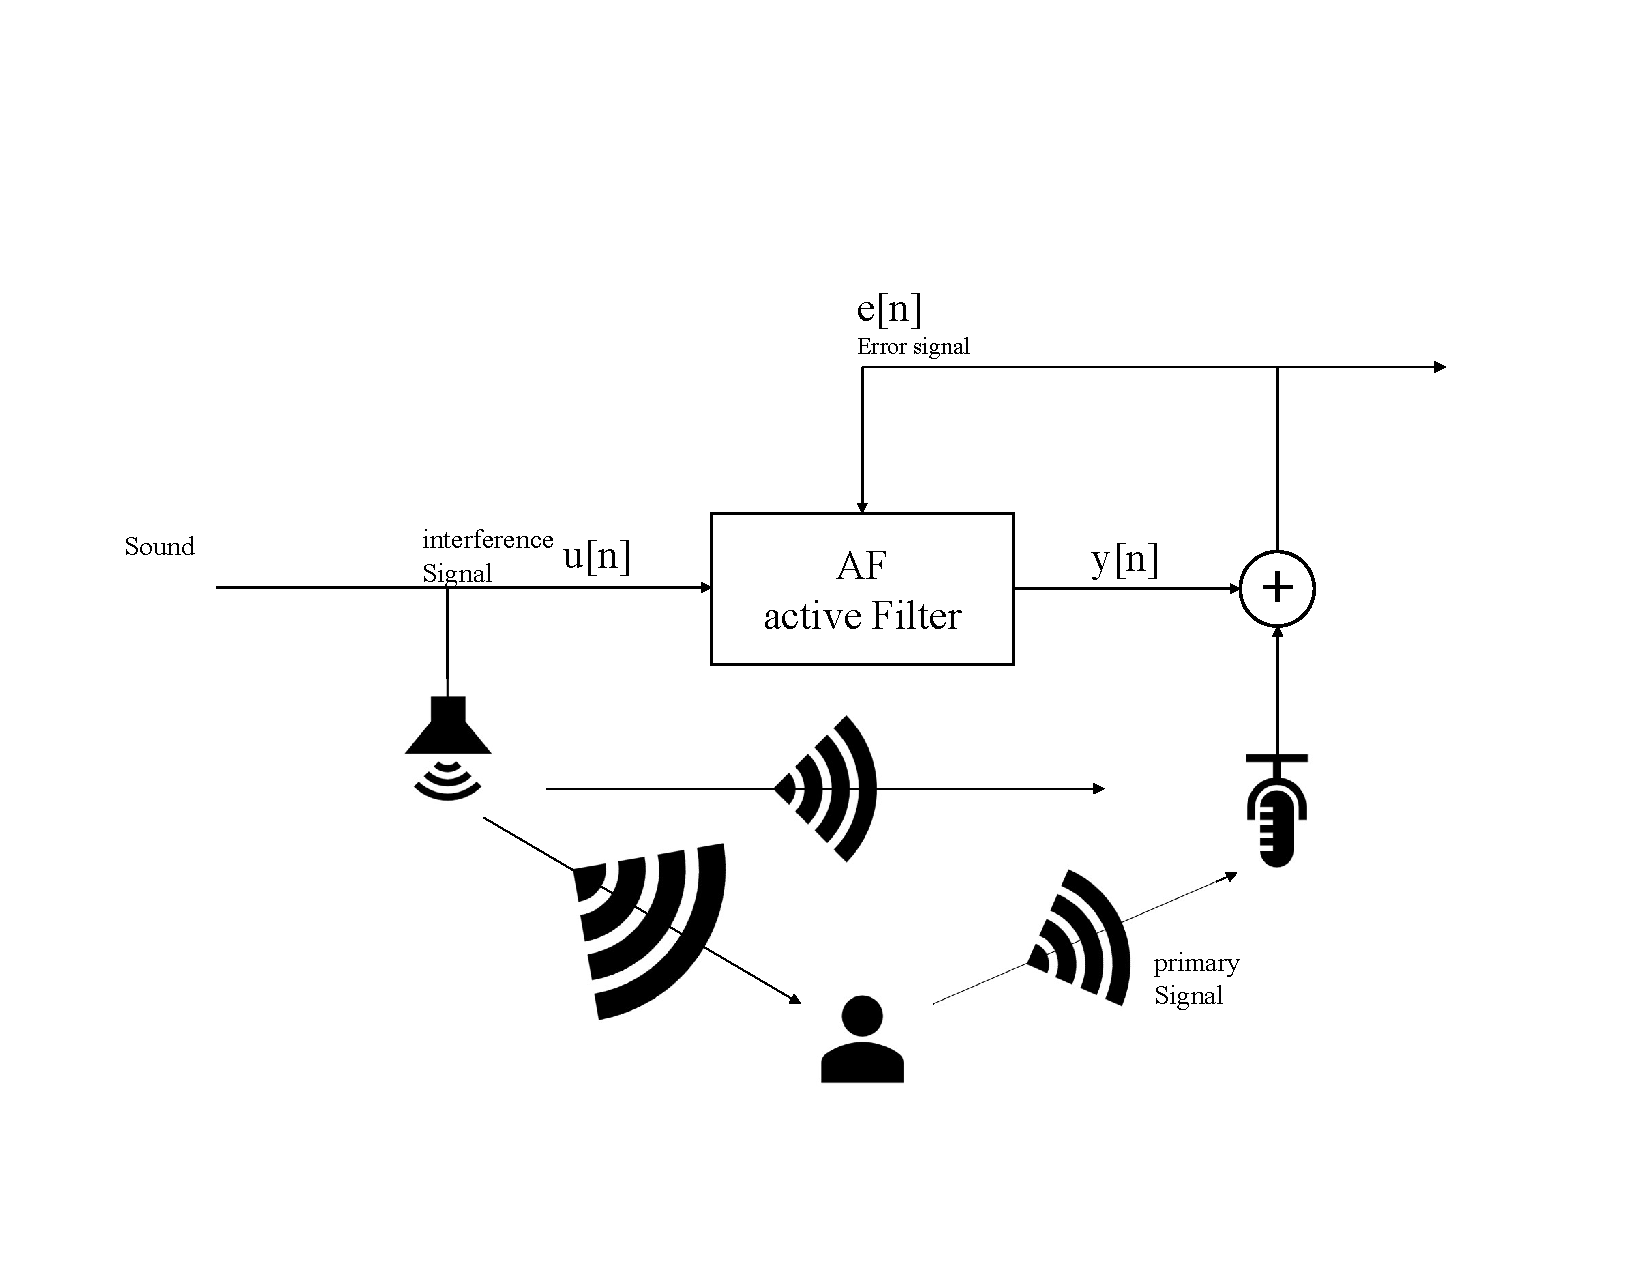
\includegraphics[scale=0.65, trim=0cm 3cm 0cm 4.5cm, clip]{interference_chanellation2.pdf}
	\caption{Example for an application for a an interference-cancelling-filter}
	\label{interference2} 
\end{figure}
For \ref{interference2}: Linear filters are better than nonlinear ones for this case. Filter tries to "'kill"' the interference because it knows, what has been played on the speaker.

\subsubsection{Complex Envelope}

\mybox{
\textbf{Definition:} 

$x(t)=\Re{u(t)e^{\j 2 \pi f_0 t}}$ 

with   
\begin{itemize}
\item $x(t)\in \mathbb{R}$: Real Signal
\item $u(t)\in \mathbb{R}$: Complex Envelope of $x(t)$
\item $f_0$: Center of Frequency; \quad $[f_0]=1 Hz$
\end{itemize}}

Notation with Magnitude and phase:

\quad $u(t)=|u(t)|\cdot e^{j\varphi_u(t)}$

Complex Envelope $u(t)$ mapped on signal $x(t)$ 

\quad $x(t)=\Re{u(t)e^{\j 2 \pi f_0 t}}=|u(t)|\cdot \cos (2\pi f_0 t + \varphi_u(t))=\frac{1}{2}u(t)\cdot e^{\j 2 \pi f_0 t}+\frac{1}{2}u^*(t)\cdot e^{-\j 2 \pi f_0 t}$

\with $\Re{z}=\frac{z+z^*}{2}$

approach to map signal $x(t)$ on complex envelope $u(t)\overset{?}{=}2x(t)\cdot e^{-j2 \pi f t }$  

\quad $2 x(t) \cdot e^{-j2 \pi f t } = 2 \Re{u(t)e^{\j 2 \pi f_0 t}}\cdot e^{-j2 \pi f t } =(u(t)e^{\j 2 \pi f_0 t} +u^*(t)e^{-\j 2 \pi f_0 t})\cdot e^{-j2 \pi f t }$

\quad $2 x(t) \cdot e^{-j2 \pi f t }  = u(t) + u^*(t)\cdot e^{-j4\pi f_0 t}$

Check approach with the Fourier transform:

$2 x(t) \cdot e^{-j2 \pi f t } \quad\laplace\quad U(f)+\int\limits_{-\infty}^{\infty}u^*(t)\cdot e^{-\j 4 \pi f_0 t}e^{\j 2 \pi f t}dt$


\with $\int\limits_{-\infty}^{\infty}u^*(t)\cdot e^{-\j 4 \pi f_0 t}e^{\j 2 \pi f t}dt 
=\int\limits_{-\infty}^{\infty}u^*(t)\cdot e^{-\j 2 \pi (f+2f_0) t}dt
=\left(\int\limits_{-\infty}^{\infty}u(t)\cdot e^{-\j 2 \pi (f+2f_0) t}\right)^*$

\qquad$=\left(\left.\underbrace{\int\limits_{-\infty}^{\infty}u(t)\cdot e^{-\j 2 \pi (f+2f_0) t}}_{U(f)}\right|_{-f-2f_0\to f }\right)^*=U^*(-f-2f_0)$

\pfeil $2 x(t) \cdot e^{-j2 \pi f t } \quad\laplace\quad U(f)+U^*(-f-2f_0)$

\begin{figure}[H]
	\centering
	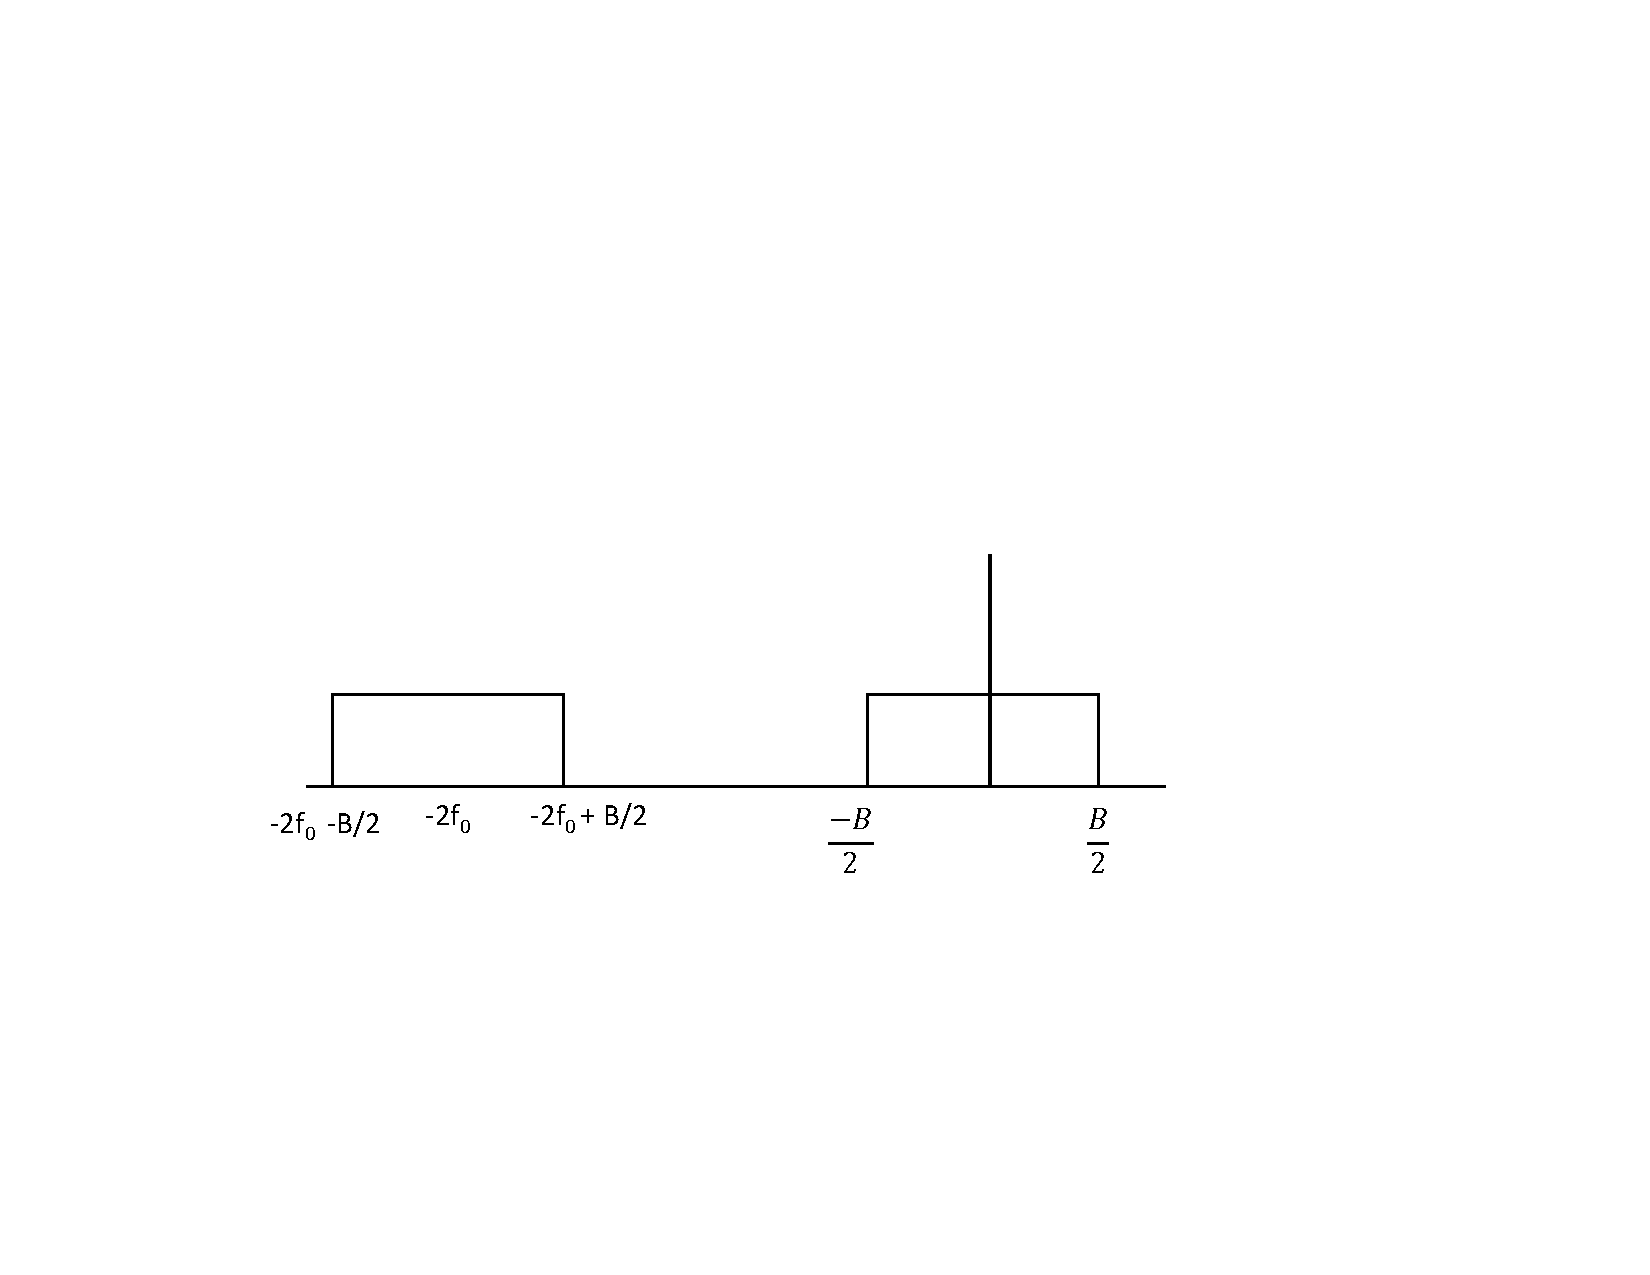
\includegraphics[scale=0.65, trim=0cm 6cm 0cm 11cm, clip]{bandlimitation.pdf}
	\caption{Result of the Fourier Transform}
	\label{ResultFourier} 
\end{figure}


\ \\
The result shows an additional shifted envelope \pfeil therefore a low pass filter (LPF) is needed to suppress overlapping (aliasing).\pfeil band limitation\\
\pfeil $u(t) = LPF( x(t) \cdot 2\cdot e^{-j2 \pi f t } )$
\ \\$x(t) \iff u(t)$ $[$It's not a Fourier transform, but related.$]$\\

\textbf{Constraints for Bandwidth:}

Out of Picture \ref{ResultFourier}:

\quad $-2f_0+\frac{B}{2} \leq -\frac{B}{2} $ 

\mybox{
\pfeil  $B \leq 2 f_0$ \qquad or \qquad $f_0 \geq \frac{B}{2}$}


\begin{figure}[H]
	\centering
	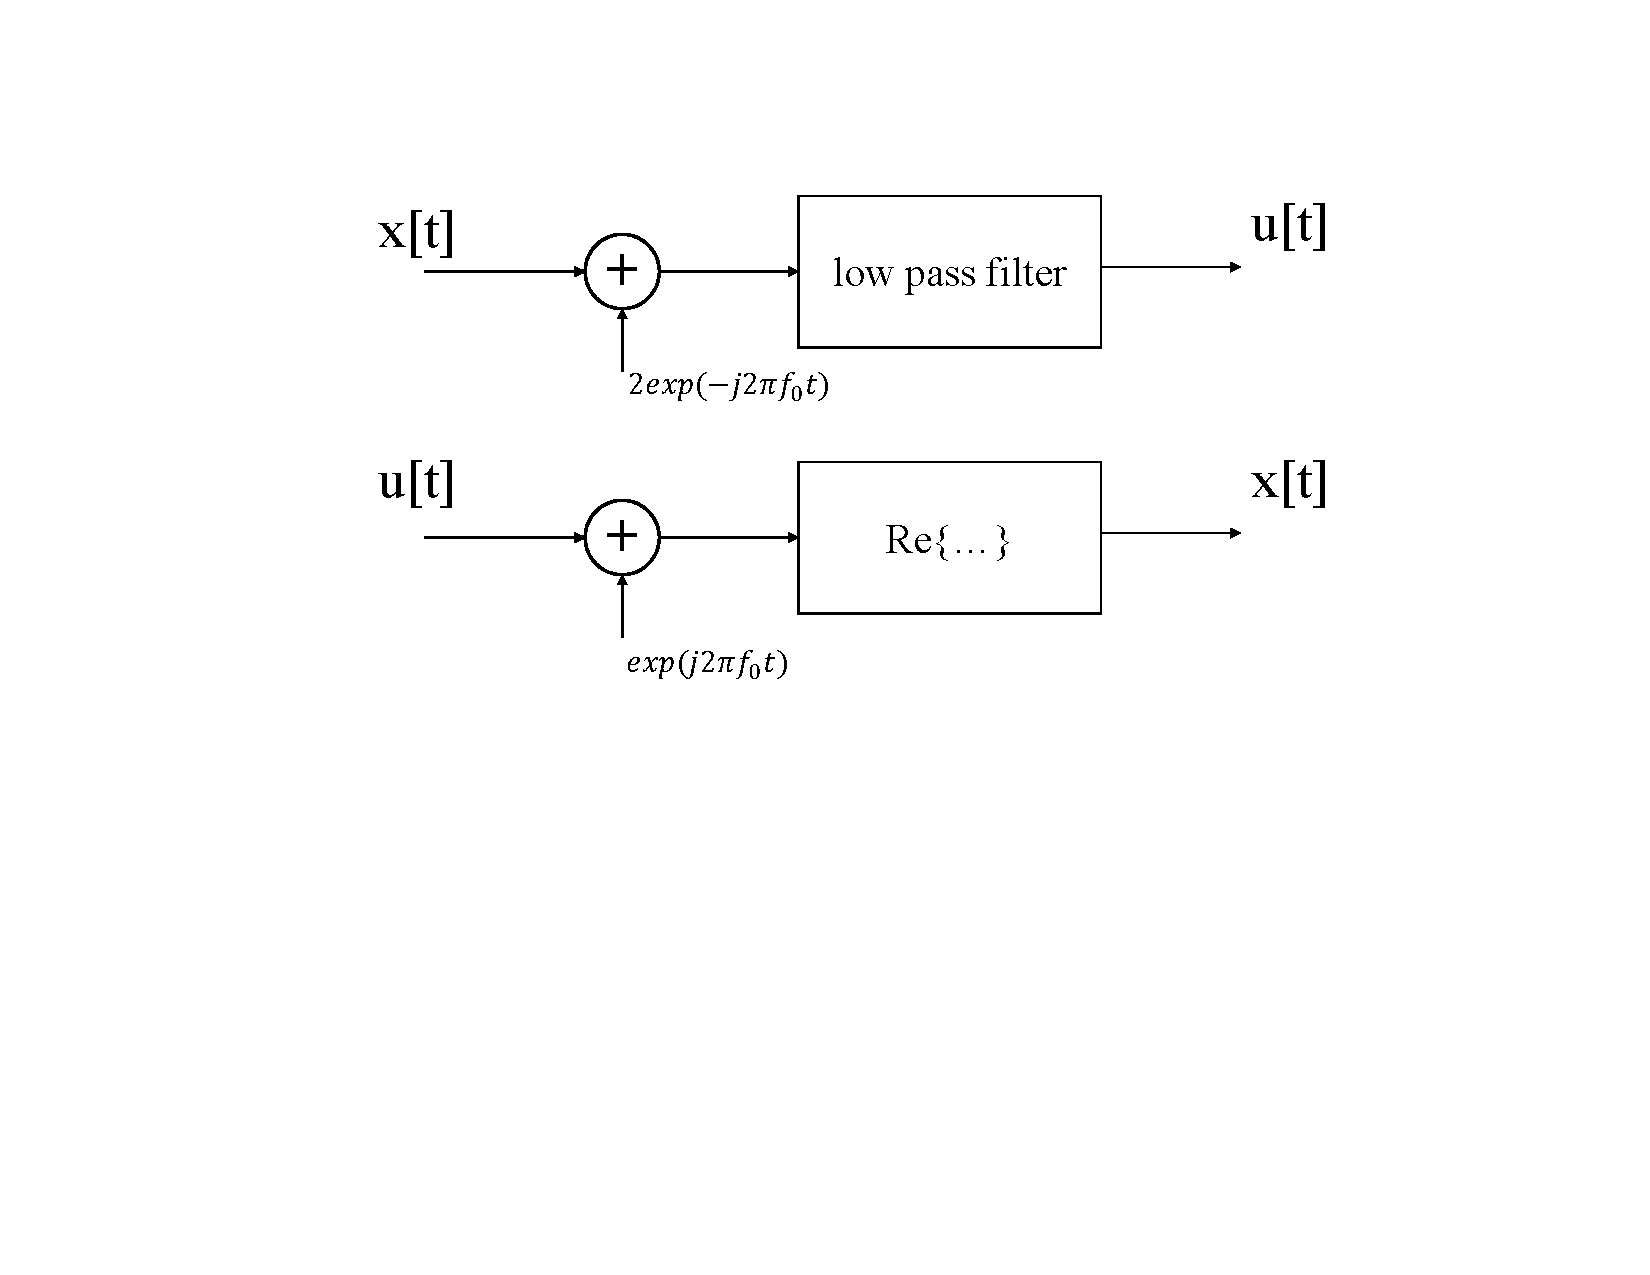
\includegraphics[scale=0.65, trim=0cm 10cm 0cm 3cm, clip]{bandpass_not_overlapping.pdf}
	\caption{Transformation from complex envelope and signal as block diagram and vice versa}
	\label{complexEnvelopTransform} 
\end{figure}
$x(t) \iff u(t)$ $[$It's not a fourier transform, but related.$]$\\
\ \\

\subsubsection{Whatever we did here - No. 264}
\paragraph{\texorpdfstring{Ivrla\v c}{Ivrlac} the dimensions Conqueror }

\[\sum_{m}\underbrace{a_m}_{\in \mathbb{R}}x(t-t_m) \iff \sum_{m}\underbrace{a_m \cdot e^{-i 2\pi f_0 t_m}}_{b_m \in \mathbb{C}}u(t-t_m)  = \sum_{m} |b_m| \cdot e^{j\varphi_m} u(t-t_m)\] \\
Under condition of:$\vert b_m\vert = a_m \quad  \varphi_{b_m}= -2\pi f_0 t_m$\\
Note: Correspondence is linear; center frequency has to be known.\\

\begin{doublespace} 
$u(t) \iff x(t) = \Re { u(t) e^{j2\pi f_0 t} }$\\
\paragraph{Approach - Complex Envelope shifted and scaled to fit a real signal}\ \\
$w^* u(t-\tau) \ct c\cdot x(t-\overset{\sim}{t}) = x'(t) \with c \in \mathbb{R}$



$\underbrace{w^*}_{const.}\cdot u(t-\tau)$  $\ct x'(t)= \Re {w^*\cdot u(t-\tau) e^{j2\pi f_0 t}},\\ \with \quad u(t)= |u(t)| e^{j2\pi f_0 (t-\tau)} \quad w=|w|e^{j\varphi_w}$\\


$c\cdot x(t-\tau)= \Re{w^* u(t-\tau e^{j2\pi f_0 t})}$

$c\cdot \Re{u(t-\overset{\sim}{t})\cdot e^{j2\pi f_0(t-\overset{\sim}{t})}}  = \Re{w^*\cdot u(t-\tau)\cdot e^{j2\pi f_0 t}} $\\
$c \cdot |u(t-\overset{\sim}{t})|\cos(2\pi f_0t-2\pi f_0 \overset{\sim}{t} + \varphi_u(t-\overset{\sim}{t})) = |w||u(t-\tau)|\cos(2\pi f_0 t + 2\pi \varphi_u (t-\tau)-\varphi_w)$\\
\pfeil cos(arg) should be equal!\\
$2\pi f_0t-2\pi f_0 \overset{\sim}{t} + \varphi_u(t-\overset{\sim}{t}) = 2\pi f_0 t + 2\pi \varphi_u (t-\tau)-\varphi_w$\\
$2\pi f_0t-2\pi f_0 \overset{\sim}{t} + \varphi_u(t-\overset{\sim}{t}) = 2\pi f_0 t + 2\pi \varphi_u (t-\tau)-\varphi_w+ q\cdot2\pi \with q \in \mathbb{Z}$\\
$f_0 \tilde{t}=\frac{\varphi_u(t-\tilde{t})-\varphi_u(t-\tau)+\varphi_w}{2\pi}-q$\\
Non-linear in $\tilde{t}$\\
Substitution: $\tilde{t}=\tau+\Delta t$ \\
$f_0 \Delta t=\frac{\varphi_u(t-\overset{\sim}{t}-\Delta t)-\varphi_u(t-\tau)+\varphi_w}{2\pi}-f_0\tau-q$\\
\textbf{Choose} q:\\
$0\leq f_0 \Delta t <1$\\
\begin{tabular}{ll}
\textbf{Assumption}: & u(t) is \textbf{narrow band}\\ 
 &$u(t-t')\approx u(t)$ \with $|t'|\leq \frac{1}{f_0}$\\
 &$f_0 \Delta t = (\frac{\varphi_w}{2\pi}-f_0\tau)mod(1)$\\
 &$\Delta t= (\frac{\varphi_w}{2\pi f_0}-\tau)mod(\frac{1}{f_0})$\\
\end{tabular}\\

\mybox{
$\tilde{t}= (\frac{\varphi_w}{2\pi f_0}-\tau)mod(\frac{1}{f_0})+\tau$\\
$c=|w|$ Complex envelope only for narrow band!}
\ \\


\paragraph{Power computation}\ \\ 
\quad $x(t)=\frac{1}{2}u(t)\cdot e^{\j 2 \pi f_0 t}+\frac{1}{2}u^*(t)\cdot e^{-\j 2 \pi f_0 t} \quad |(\bullet)^2$\\
\quad $x(t)^2=(\frac{1}{2}u(t)\cdot e^{\j 2 \pi f_0 t}+\frac{1}{2}u^*(t)\cdot e^{-\j 2 \pi f_0 t})(\frac{1}{2}u(t)\cdot e^{\j 2 \pi f_0 t}+\frac{1}{2}u^*(t)\cdot e^{-\j 2 \pi f_0 t})$\\
\quad $x(t)^2=\frac{1}{4}u^2(t)\cdot e^{\j 4 \pi f_0 t}
+\frac{1}{2}u(t)\cdot u^*(t)+
\frac{1}{4}u^{2*}(t)\cdot e^{-\j 4 \pi f_0 t}$\\
\with $\frac{1}{2}u(t)\cdot u^*(t)=\frac{1}{2}|u(t)|^2 $\\
$ \with \frac{1}{4}u^2(t)\cdot e^{\j 4 \pi f_0 t}+\frac{1}{4}u^{2*}(t)\cdot e^{-\j 4 \pi f_0 t}=\frac{1}{4}u^2(t)\cdot e^{\j 4 \pi f_0 t}+(\frac{1}{4}u^{2}(t)\cdot e^{\j 4 \pi f_0 t})^*=\frac{1}{2}\Re{u^2(t)e^{j4\pi f_0t}}$\\
Square of Magnitude\\
$|x(t)|^2= \frac{1}{2}|u(t)|^2 + \frac{1}{2}\Re{u^2(t)e^{j4\pi f_0t}}$\\
Get Time average with expectation:\\
Restrict u(t) to be proper:\\
$E[u^2(t)]=0$\\ $E[|x(t)|^2]=\frac{1}{2}E[|u(t)|^2]$\\
$u(t)= a(t)+jb(t)$\\
$u^2(t)= a^2(t) + 2j a(t)b(t) -b^2(t)$\\
$E[u^2]= \underbrace{E[a^2(t)-b^2(t)]}_{=0}+\underbrace{2jE[a(t)b(t)]}_{=0}\overset{!}{=}0$ \quad (widely linear processing)\\
\textbf{Mean Time square average for narrow band:}  (equals power)\\
$\overline{x^2(t)}=f_0 \cdot\int\limits_{t-\frac{1}{2f_0}}^{t+\frac{1}{2f_0}}x^2(\tau) d\tau \approx \frac{1}{2}|u(t)|^2 $\\
time average $x^2$ is a good assumption. \pfeil We will stick with narrow band assumption \pfeil both will work.\\
\end{doublespace}

\subsubsection{FIR-Filter}
\begin{figure}[H]
	\centering
	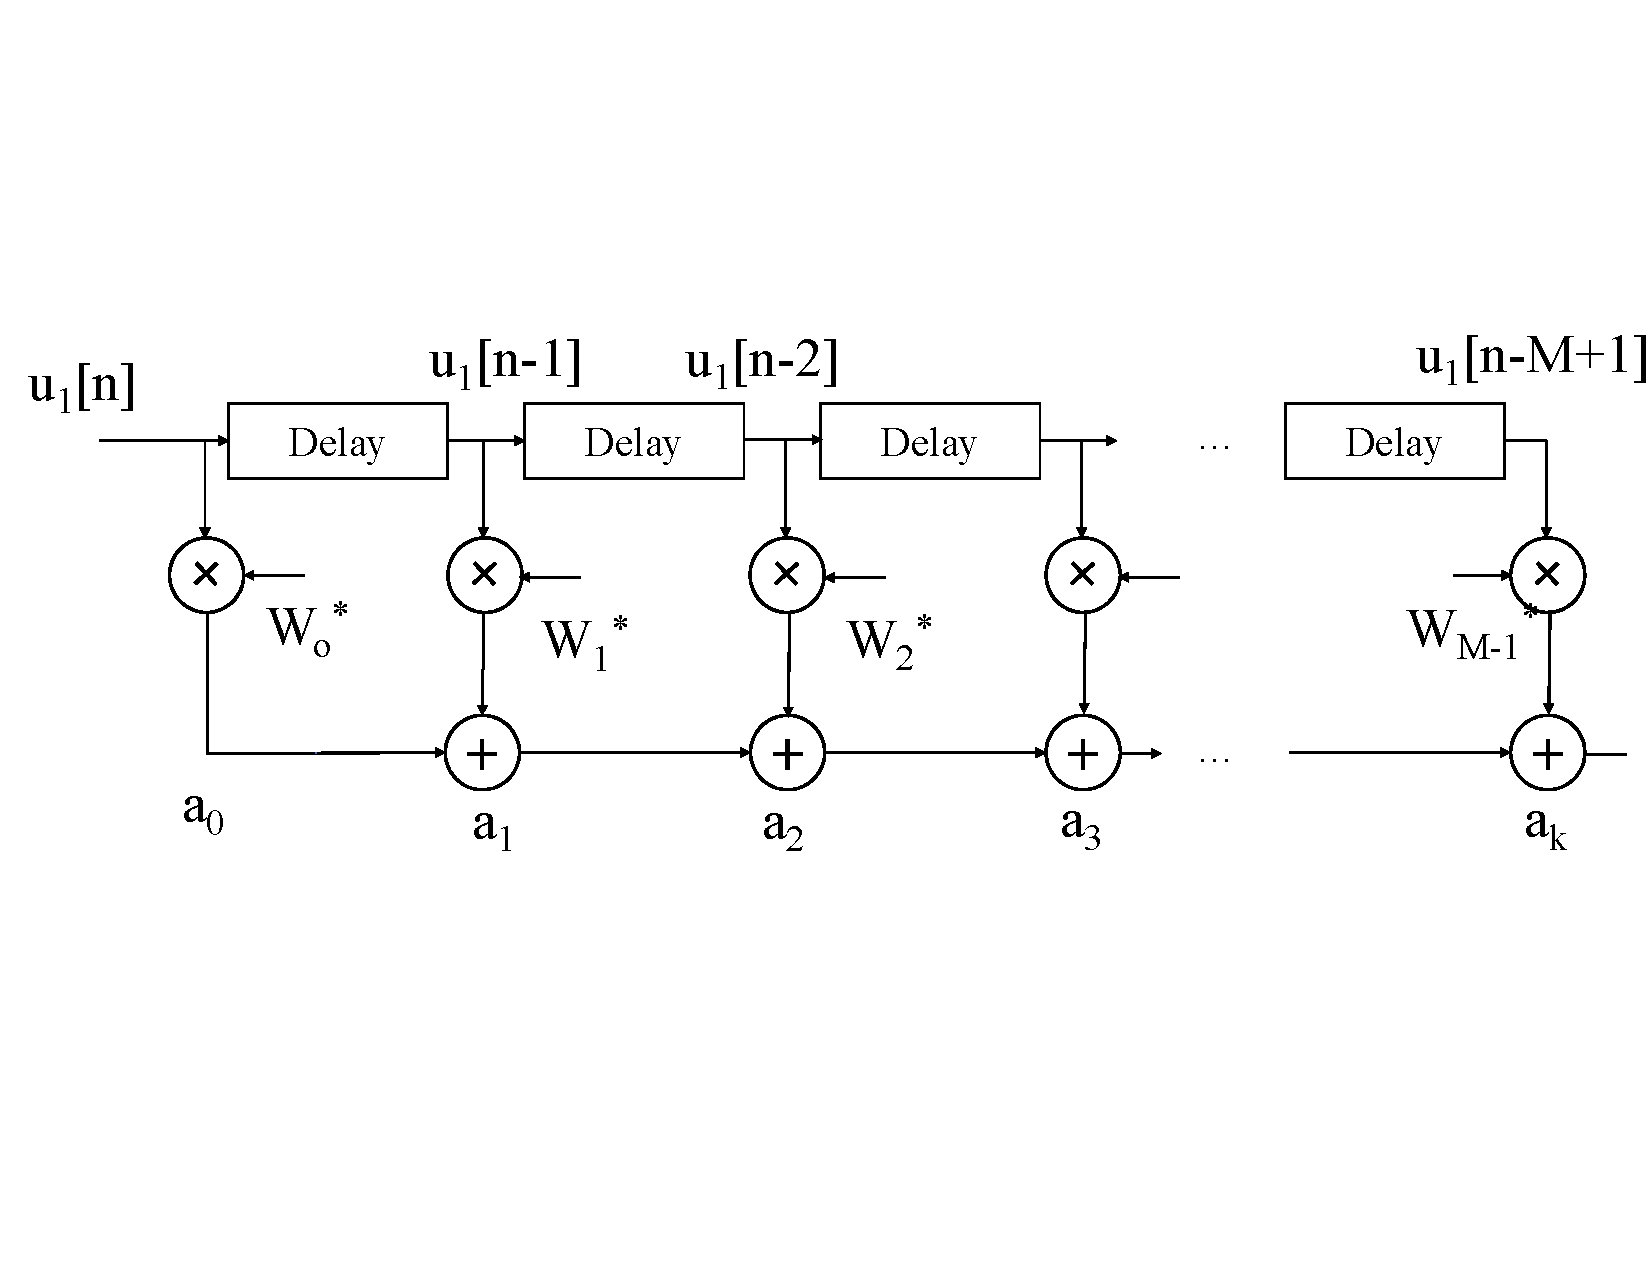
\includegraphics[scale=0.65, trim=0cm 7cm 0cm 3cm, clip]{delay_filter2.pdf}
	\caption{stable, finite response}
	\label{delay2} 
\end{figure}

\begin{doublespace}
$\vec{w}= \left[\begin{array}{c}
w_0\\ w_1\\ .\\.\\. \\ w_{M-1}
\end{array}\right] \in \mathbb{C}^{M\times 1}$; \qquad $\vec{w}^*= \left[\begin{array}{c}
w_0^*\\ w_1^*\\ .\\.\\. \\ w_{M-1}^*
\end{array}\right]$\\ \\
$\vec{w}^T= \left[\begin{array}{c c c c}
w_0& w_1& ...&w_{M-1}
\end{array}\right]$\\
$(\vec{w}^T)^*=(\vec{w}^*)^T= \vec{w}^H$\\

$\vec{u}[n]= \left[\begin{array}{c}
u[n]\\ u[n-1]\\ .\\.\\. \\ u[n-M+1]
\end{array}\right] \in \mathbb{C}^{M\times 1}$\\ \\
$y[n]= \vec{w}^H \cdot \vec{u}[n] = u[n]w_0^*+ u[n-1]w_1^* + ... + u[n-M+1]w_{M-1}^*$\\
$y^*[n]= (\vec{w}^H\vec{u}[n])^*= (( \vec{w}^H \vec{u}[n])^T)^*= (\vec{w}^H \vec{u}[n])^H= \vec{u}^H[n]\vec{w}$\\ \\
$\vec{y}[n]= \left[\begin{array}{c}
	\vec{y}[n]\\ \vec{y}[n+1]\\ .\\.\\. \\ \vec{y}[n+N]
\end{array}\right]\in \mathbb{C}^{(N+1)\times 1}$\\ \\

$\vec{d}[n]= \left[\begin{array}{c}
d[n]\\ d[n+1]\\ .\\.\\. \\ \d[n+N]
\end{array}\right]\in \mathbb{C}^{(N+1)\times 1} \qquad \vec{d} $ is the desired signal\\ \\ \ \\
\textbf{error:} $\vec{e}[n]= \vec{d}[n]-\vec{y}[n]$\\ \ \\
$\vec{w}_{MMSE}= arg \min\limits_{\vec{w}} \underbrace{\sum_{k=0}^{N}|e[n+k]|^2}_{\vec{e}^H[n]\vec{e}[n]= ||\vec{e}[n]||_2^2 \quad \textrm{Squared Euclidean Norm}} $\\ \ \\
Note: MMSE means Minimum Mean Square Error \qquad $\vec{w}$ is the weighting coefficient\\
$\vec{w}_{LS}= arg  \min\limits_{\vec{w}} E[||\vec{e}[n]||_2^2]$ \qquad Note: LS means Least Square Error\\
$\vec{w}_{OPT}= arg  \min\limits_{\vec{w}}  E[||\vec{e}[n]||_2^2]$,\quad  such that \quad $\left\lbrace \begin{array}{l} \vec{w}_1^H\vec{a}_i=b_1\\ i \in \{1,2,...,k\} \end{array} \right.$ Constraints\\ 
OPT means Additional Constraints, Optimization.\\

$\vec{e}^*[n] = \vec{d}^*[n]-\vec{y}^*[n] = \vec{d}^*[n] -\underbrace{\left[\begin{array}{c}
\vec{u}^H[n] \\ \vec{u}^H[n+1] \\ \svdots \\ \vec{u}^H[n+N] \end{array}\right]}_{\text{Signal Matrix }\ma{U}^H[n]} \vec{w} = \vec{d}^*[n]-\ma{U}^H[n]\vec{w}$\\
  
\begin{tabular}{lll}
$||\vec{e}[n]||^2_2=$&$\vec{e}^H[n]\vec{e}[n]$ &$=(\vec{e}^H[n]\vec{e}[n])^*$ (\footnotesize Note: It's a real number, so complex conjungation doesn't hurt!\normalsize) \\
 &&$= (\vec{e}^*[n])^H\vec{e}^*[n]= (\vec{d}^*[n]+\ma{U}^H\vec{w})^H(\vec{d}^*[n]-\ma{U}^H[n]\vec{w})$\\
 &&$= ((\vec{d}^*[n]^H-\vec{w}^H\ma{U}[n])(\vec{d}^*[n]-\ma{U}^H[n]\vec{w}))$\\
 &&$= ||\vec{d}^*[n]||^2_2 -\underbrace{(\vec{d}^*[n])^H\ma{U}^H[n]}_{\vec{\rho^H}}\vec{w}-\vec{w}^H\underbrace{\ma{U}[n]\vec{d}^*[n]}_{\vec{\rho}}+\vec{w}\underbrace{\ma{U}[n]\ma{U}^H[n]}_{\ma{R}=\ma{R}^H}\vec{w}$\\
\end{tabular}
\end{doublespace}
\mybox{Minimization of quadratic forms\\ $||\vec{e}[n]||^2_2=\vec{w}^H\ma{R}\vec{w}- \vec{\rho}^H\vec{w}-\vec{w}^H\vec{\rho}+||\vec{d}[n]||^2_2 \qquad \in \mathbb{R}$ }
\subsubsection{Spatial Filtering}
\paragraph{Planar wave}
\begin{figure}[H]
	\centering
	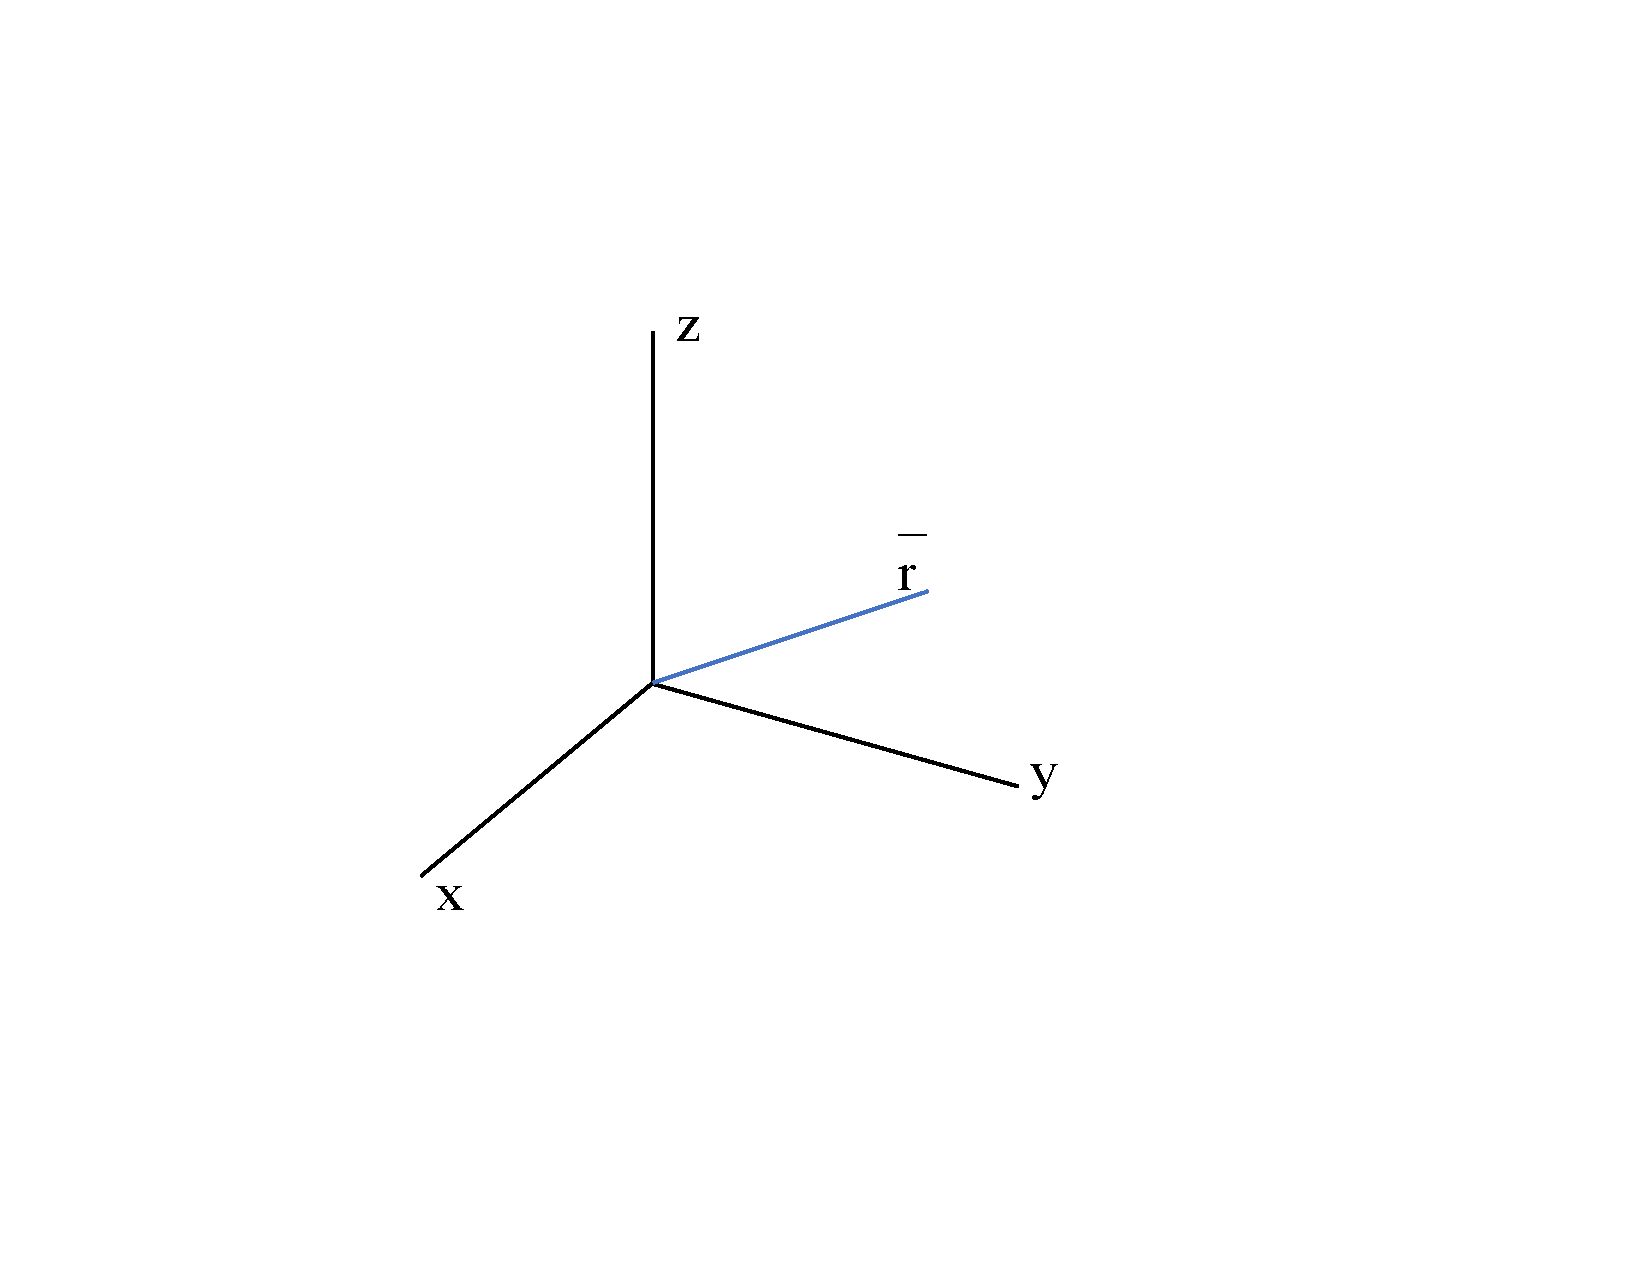
\includegraphics[scale=0.65, trim=0cm 5cm 0cm 4cm, clip]{planarwave.pdf}
	\caption{Direction of planar wave}
	\label{planarwave} 
\end{figure}
$\underbrace{q(t,\vecp{r})}_{field}=F(t-\frac{\vecp{n}\cdot \vecp{r}}{c})$\\
$\vecp{n}\cdot \vecp{n}=1; \quad c=const >0 \qquad$ \vecp{n}= direction of propagation\\ \ \\
\textbf{Property 1}\\
$\forall \Delta \vecp{r}: \Delta \vecp{r} \cdot \vecp{n} = 0 \quad \pfeil q(t,\vecp{r}+\Delta \vecp{r})= q(t,\vecp{r})$\\
"Planar"
\begin{figure}[H]
	\centering
	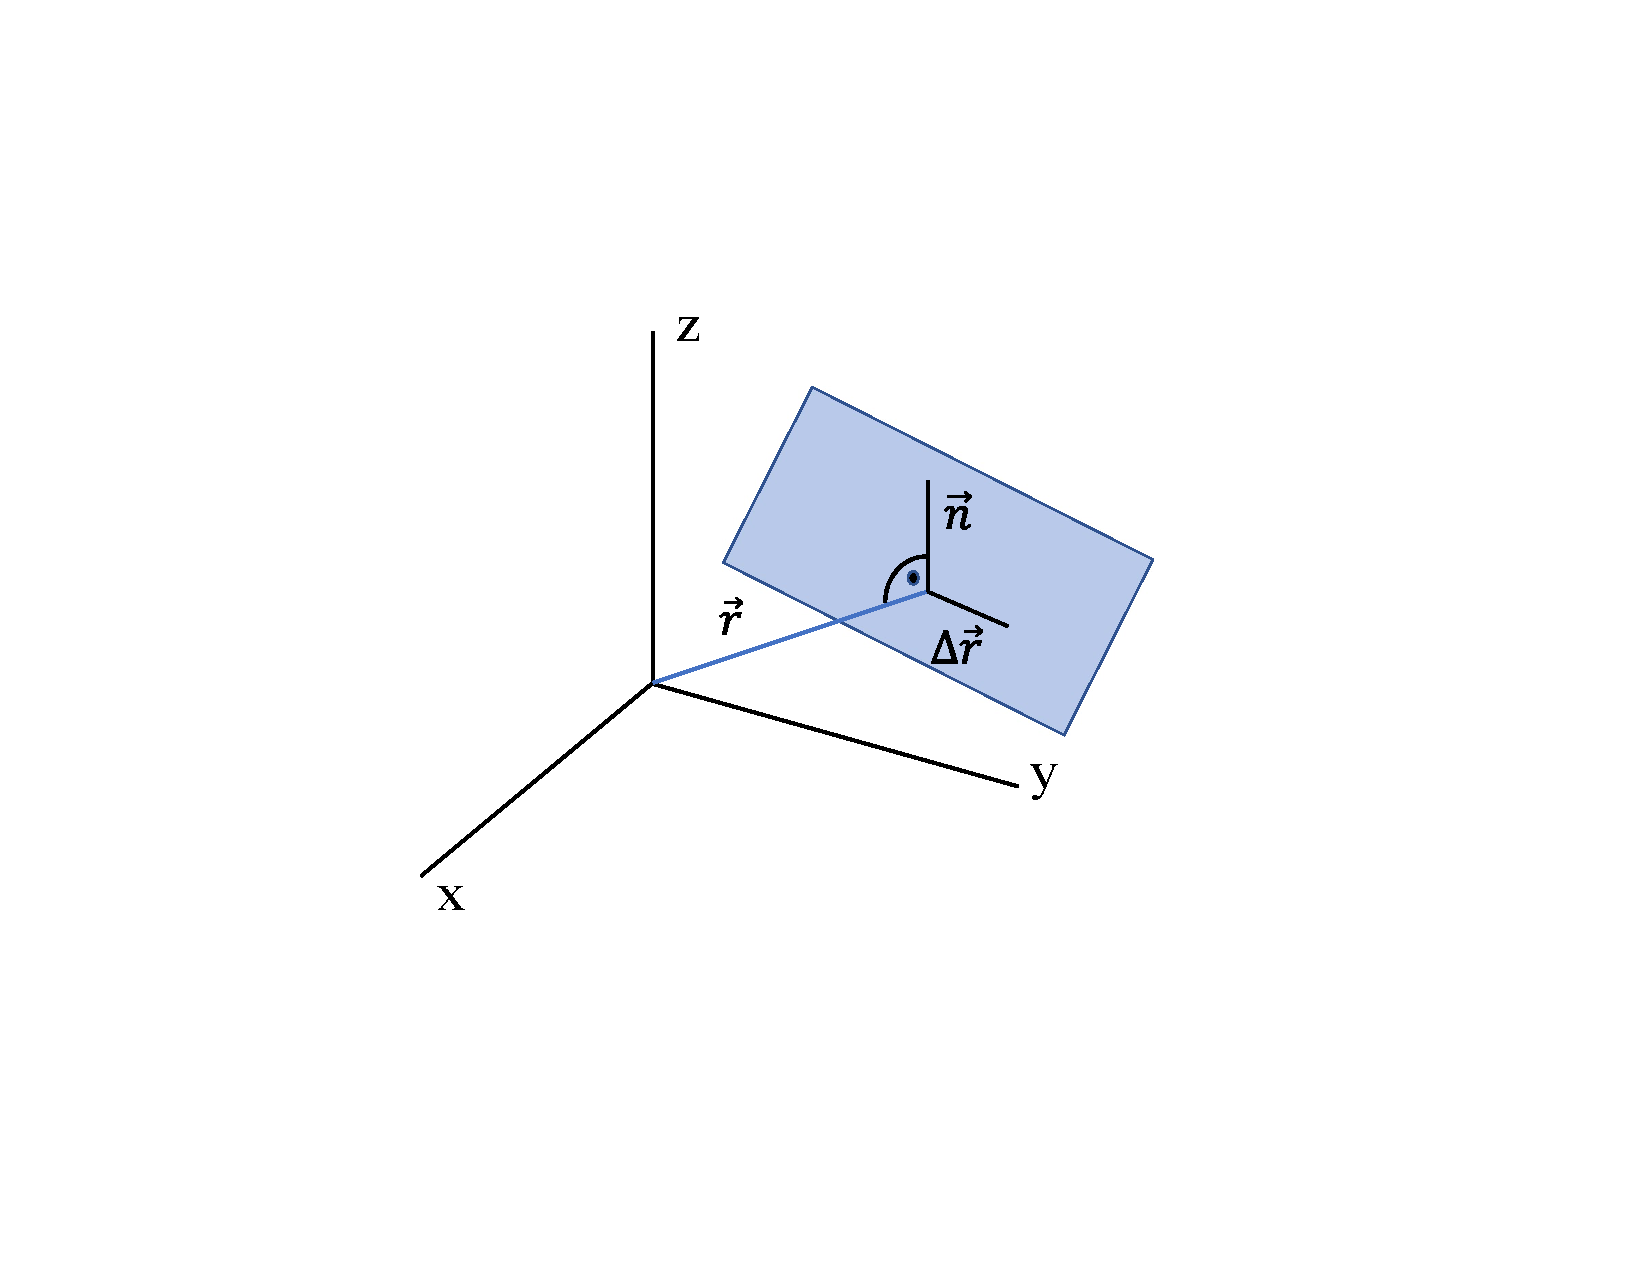
\includegraphics[scale=0.65, trim=0cm 5cm 0cm 4cm, clip]{plane.pdf}
	\caption{plane in space}
	\label{plane} 
\end{figure}

\textbf{Property 2}\\
\begin{doublespace}
$q(t+\Delta t, \vecp{r} + \Delta t\cdot c \vecp{n}) \equiv q(t,\vecp{r})$\\
Moving of $q(t,\vecp{r})$ into direction of $\vecp{n}$ with speed $c$.\\

\texttt{Harmonic planar wave:}\\
$F(\tau)= A \cos(2\pi f_0\tau +\varphi ) \qquad A, f_0, \varphi = const.$\\ 
$q(t,\vecp{r})= A \cos(2\pi f_0(t-\frac{\vecp{n}\cdot\vecp{r}}{c})+\varphi) = \Re{u(\vecp{r})e^{(j2\pi f_0t)}}$\\
$u(\vecp{r})= \underbrace{A e^{(j\varphi)}}_{S \in \mathbb{C}; s = const.} e^{(-j2\pi f_0 \frac{\vecp{n}\cdot\vecp{r}}{c})}$\\ \ \\
\textbf{Property 3}\\
$u(\vecp{r}+ \frac{c}{f_0}\vecp{n})\equiv u(\vecp{r})$ \qquad $\lambda$ wave length; $\lambda =\frac{c}{f_0} $\\ \ \\
$u(\vecp{r}) = s\cdot  e^{-j2\pi \frac{\vecp{n}\cdot\vecp{r}}{\lambda}}$\\ \ \\


$u(\vecp{r}+ l\vec{n})= u(\vecp{r})\cdot e^{-j2\pi \frac{l}{\lambda}}$\\
Phase shift, if you go into direction of wave propagation\\ \ \\ \ \\
\texttt{Modulated harmonic planar wave}\\
s is no longer constant\\
$s= s(t,\vecp{r})= s(t-\frac{\vecp{n}\cdot\vecp{r}}{c})$ \qquad remain wave \\
\end{doublespace}
\mybox{$u(\vecp{r},t)=s(t-\frac{\vecp{n}\cdot\vecp{r}}{c})e^{(-j2\pi \frac{\vecp{n}\cdot \vecp{r}}{\lambda})}$ }\\ \ \\

\subsubsection{Spatial Sampling}
\begin{doublespace}

\begin{figure}[H]
	\centering
	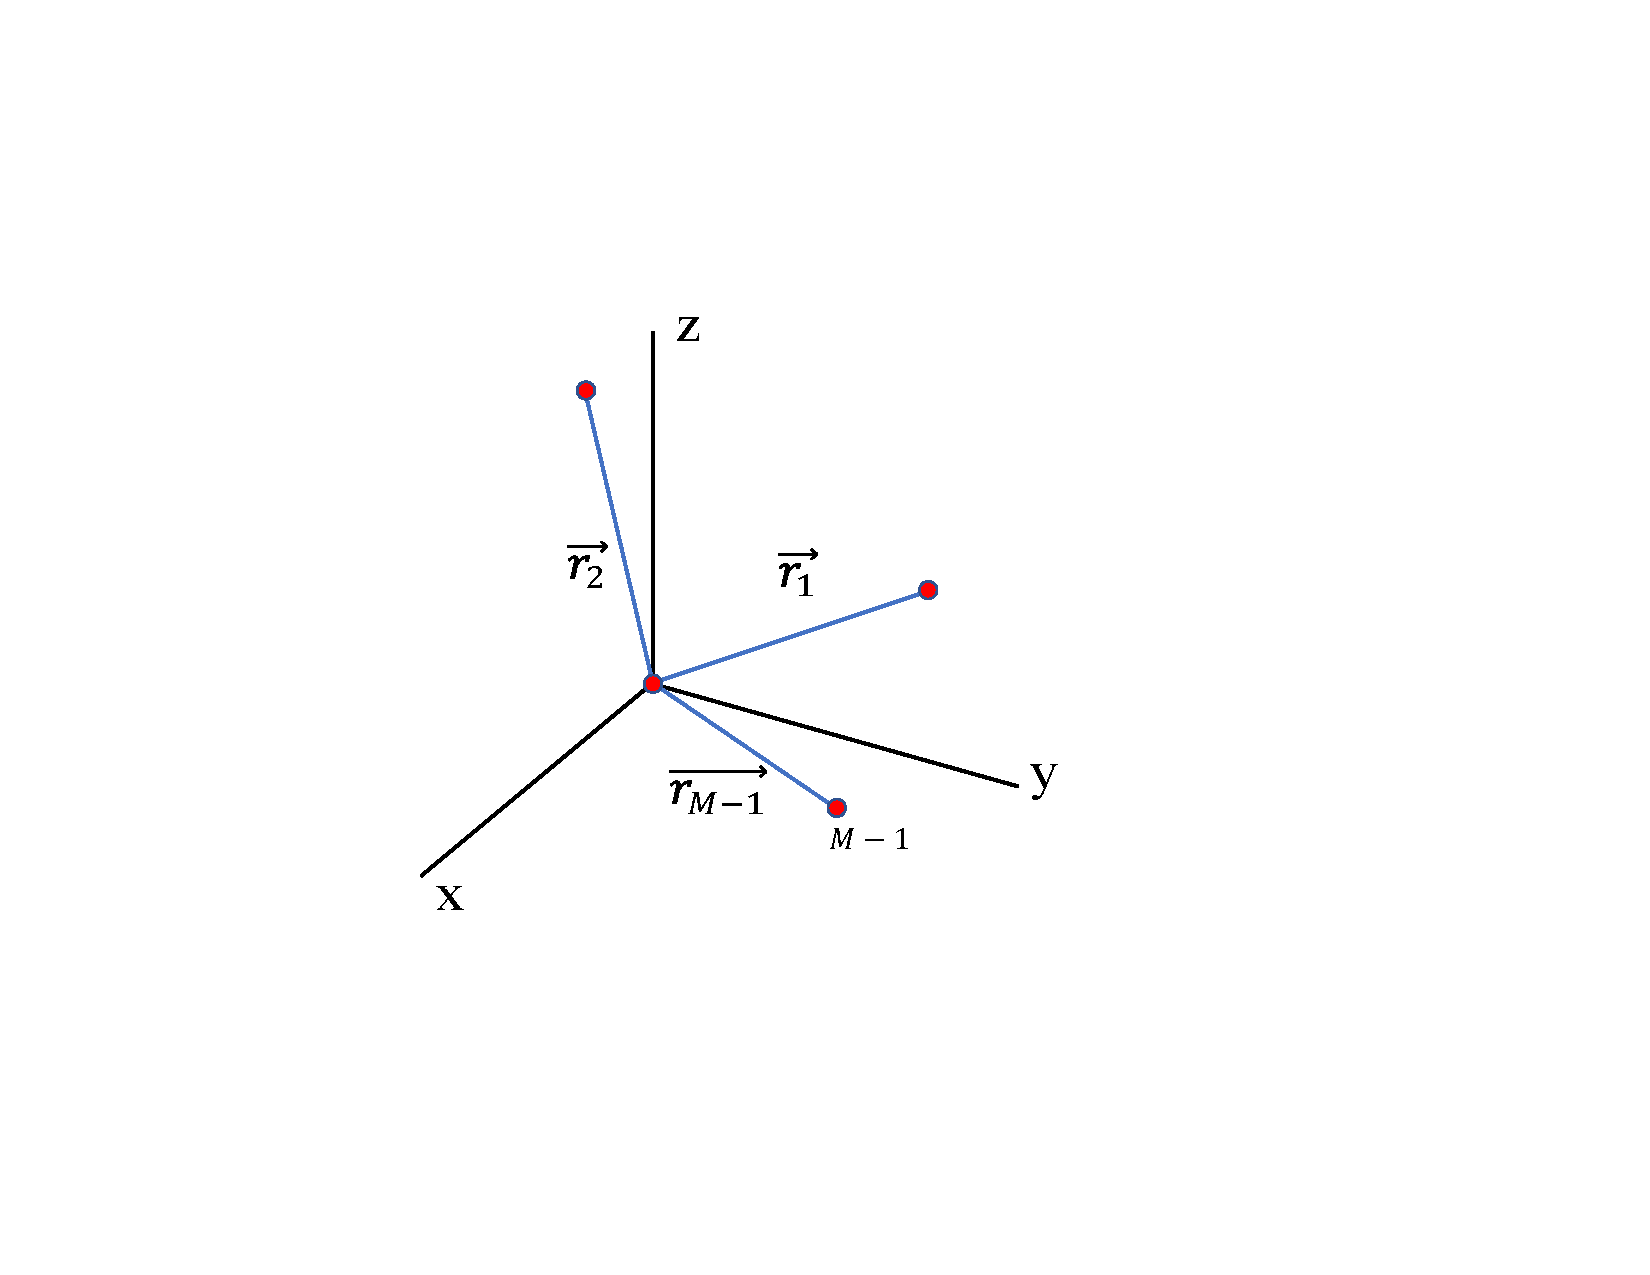
\includegraphics[scale=0.65, trim=0cm 6cm 0cm 5cm, clip]{spatialsampling.pdf}
	\caption{Spatial Sampling with M sensors}
	\label{sampling} 
\end{figure}
$\vec{u}[t]= \left[\begin{array}{c}
s(t)\\ s(t-\frac{\vecp{n}\cdot\vecp{r}_1}{c})e^{-j2\pi \frac{\vecp{n}\cdot \vecp{r}_1}{\lambda}}\\ \svdots \\s(t-\frac{\vecp{n}\cdot \vecp{r}_{M-1}}{c})e^{-j2\pi \frac{\vecp{n}\cdot \vecp{r}_{M-1}}{\lambda}} 
\end{array}\right] $\pfeil Sensor array (receive vector)\\ \ \\
Definition coherence: Coherence (physics), an ideal property of waves that enables stationary (i.e. temporally and spatially constant) interference.
\begin{itemize}
	\item coherence distance, length $l_{coh}$\\
				if $|l|\leq l_{coh} \iff s(t) \approx s(t-\frac{l}{c})$ \\
	\item assume all sensors within coherence distance. \\
$\vec{u}(t)\approx s(t) \underbrace{\left[\begin{array}{c}
	1\\ e^{-j2\pi \frac{\vecp{n}\cdot \vecp{r}_1}{\lambda}}\\ \svdots \\ e^{-j2\pi \frac{\vecp{n}\cdot \vecp{r}_{M-1}}{\lambda}}
	\end{array}\right] }_{\vec{a}(\vecp{n})  \text{ Array steering Vector}} $ \pfeil no time delay, only phase shifts
\end{itemize}
$\vec{u}(nT)=s[n]\cdot \vec{a}(\vecp{n})$\with T$=$ Sampling Time, n $=$ Sampling Index $\neq \vecp{n}$ \\
\texttt{Example:}\\
$f_0 = 2.6 GHz\qquad B=20MHz$\\
$\frac{l_{coh}}{c}<< \frac{1}{B}, \quad \frac{l_{coh}}{c}\approx\frac{1}{30B}, \quad \lambda = \frac{c}{f_0}$  \\ $l_{coh}\approx 0.5m \approx 4\lambda$\\ $u[n]$ 
\end{doublespace}

\subsubsection{Large Array}
\begin{doublespace}
$s[n-\underbrace{\frac{\tau_i}{T}}_{\text{fractioned Delay}}]= s(nT-\tau_i)\qquad \tau_i=\frac{\vecp{n}\cdot\vecp{r_i}}{c}$\\ \\
\[ s[n-\frac{\tau_i}{T}]\approx  \sum_{K=-L_1}^{L_2} a_{i,k}  \quad s[n-k]\]\\ \\
$\vec{u}[n]= \underbrace{ \begin{bmatrix}1&0&\shdots&0\\0&e^{-j2\pi \frac{\vecp{n}\cdot\vecp{r}_1}{\lambda}} \\\svdots& &\ddots&\\ 0 & \shdots &e^{-j2\pi \frac{\vecp{n}\cdot\vecp{r}_{M-1}}{c}} \end{bmatrix} 
\begin{bmatrix}\overbrace{0,...,0,}^{L_1} & 1 & \overbrace{0,...,0,}^{L_2} \\ a_{1,-L_1} & ... & a_{1,-L_2}\\ \svdots & ... & \svdots \\ a_{M-1,-L_1}& ... &a_{M-1,-L_2}\end{bmatrix}}_{\ma{A}\vecp{n}} \underbrace{\begin{bmatrix}s[n+L_1]\\ s[n+L_1-1] \\\svdots \\ s[n-L_2] \end{bmatrix}}_{\vec{s}[n]}$ \\ \ \\
$\vec{u}[n]= \ma{A}(\vec{n}) \cdot\vec{s}[n]$ \pfeil long array\\
$u[n] = \vec{a}(\vecp{n})\cdot s[n]$ \pfeil small array\\
\end{doublespace}

\subsubsection{Uniform Linear Array, ULA}
same distance in between sensors, all in one line\\

\begin{figure}[H]
	\centering
	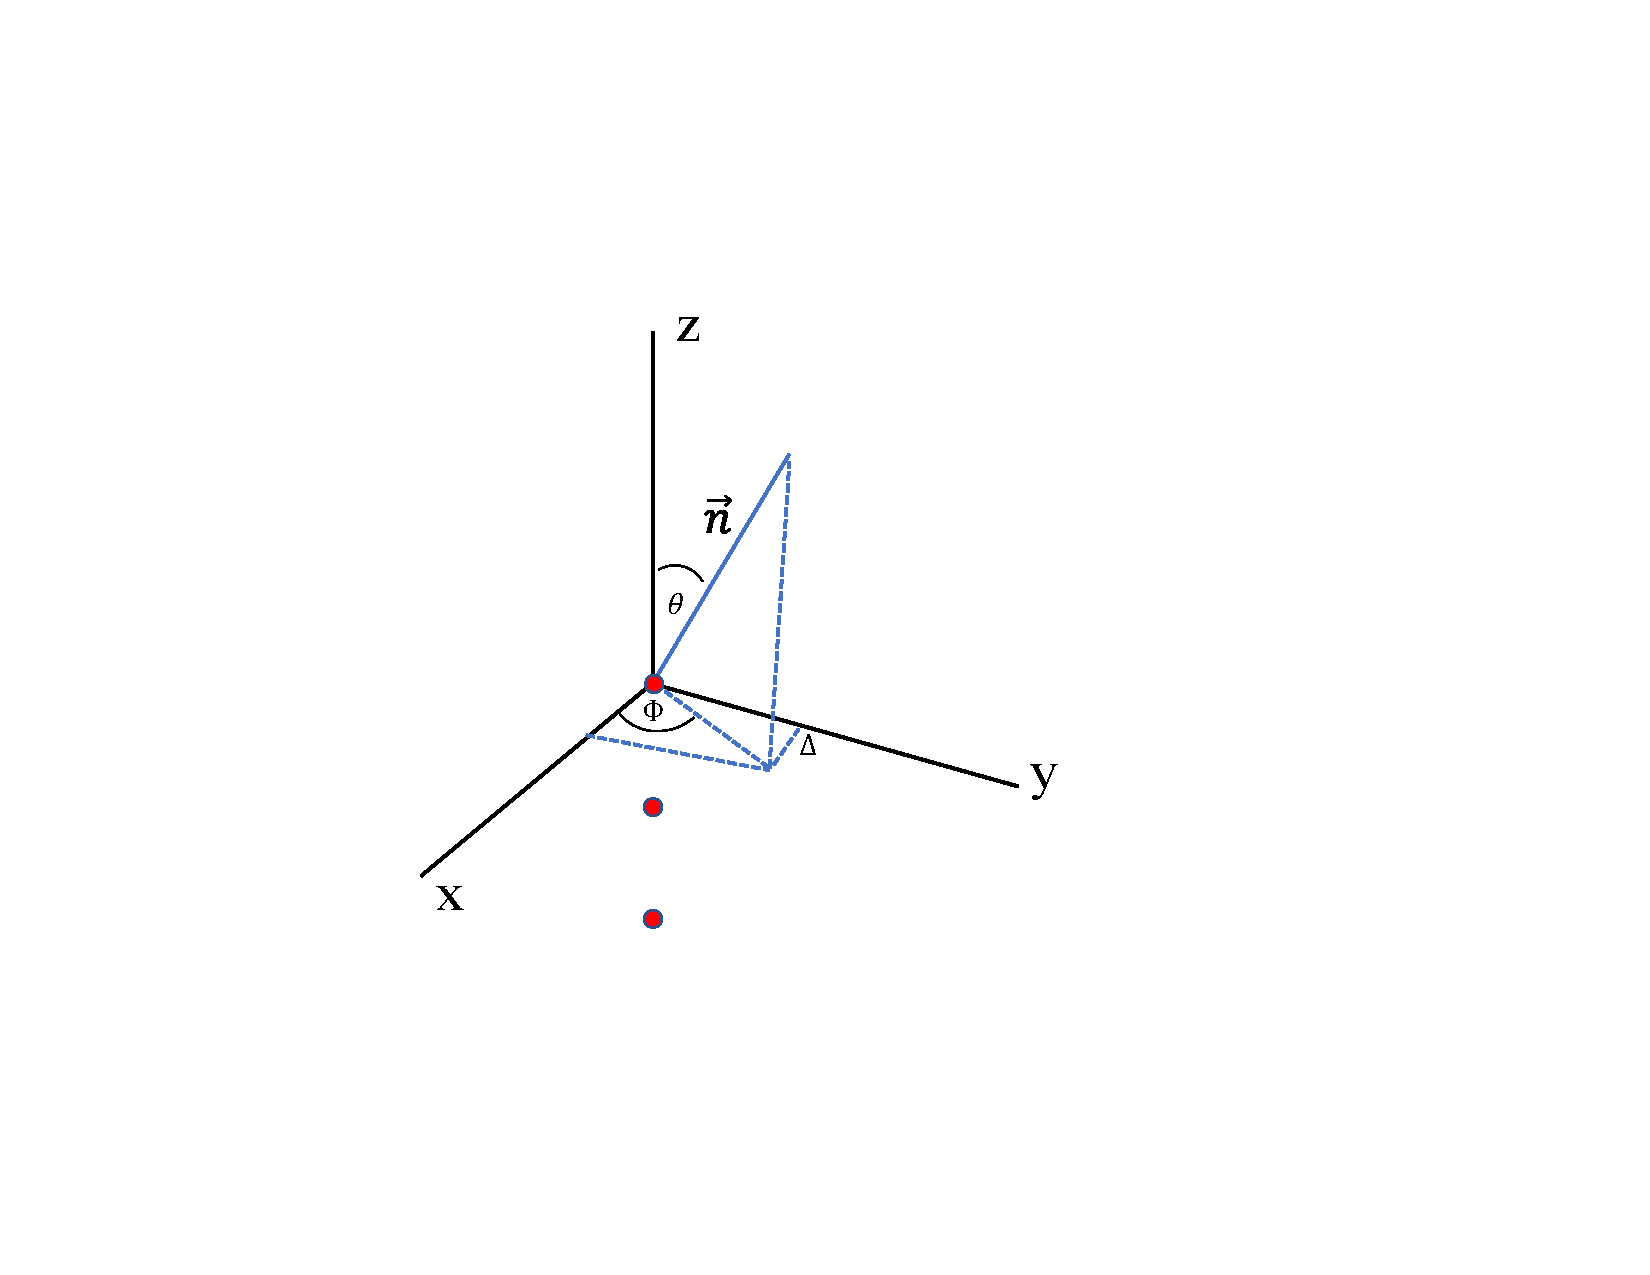
\includegraphics[scale=0.65, trim=0cm 5cm 0cm 4cm, clip]{ULA.pdf}
	\caption{Uniform Linear Array}
	\label{ula} 
\end{figure}
\begin{doublespace}
$\vecp{r}_i = -\vecp{e}_z \Delta i$ \qquad $i \in \{0,1,...,M-1\}$\\ \\
$\vecp{r}= r \begin{bmatrix}
cos \varphi sin \theta\\ sin \varphi sin \theta \\ cos \theta
\end{bmatrix}$ \qquad spherical coordinates in cartesian vector  \\ \\
$\vecp{n}=-\frac{\vecp{r}}{r}, \qquad \vecp{n}\cdot \vecp{n}=1$\\
$\vecp{r}_i\cdot\vecp{n}= - \Delta i (-\cos \Theta)= cos\Theta \cdot\Delta\cdot i$\\ \\ 
$\vec{a}(\vecp{n})= \vec{a}(\Theta)= \begin{bmatrix}1 \\ e^{-j2\pi \frac{\Delta}{\lambda}cos \Theta}\\e^{-j2\pi \frac{2\Delta}{\lambda}cos \Theta}\\ \svdots \\ e^{-j2\pi \frac{(M-1)\Delta}{\lambda}cos \Theta} \end{bmatrix}$ \qquad \pfeil Van Der Monde-Vector\\ (ULA Steering Vector)\\ \\
\end{doublespace}

\begin{figure}[H]
	\centering
	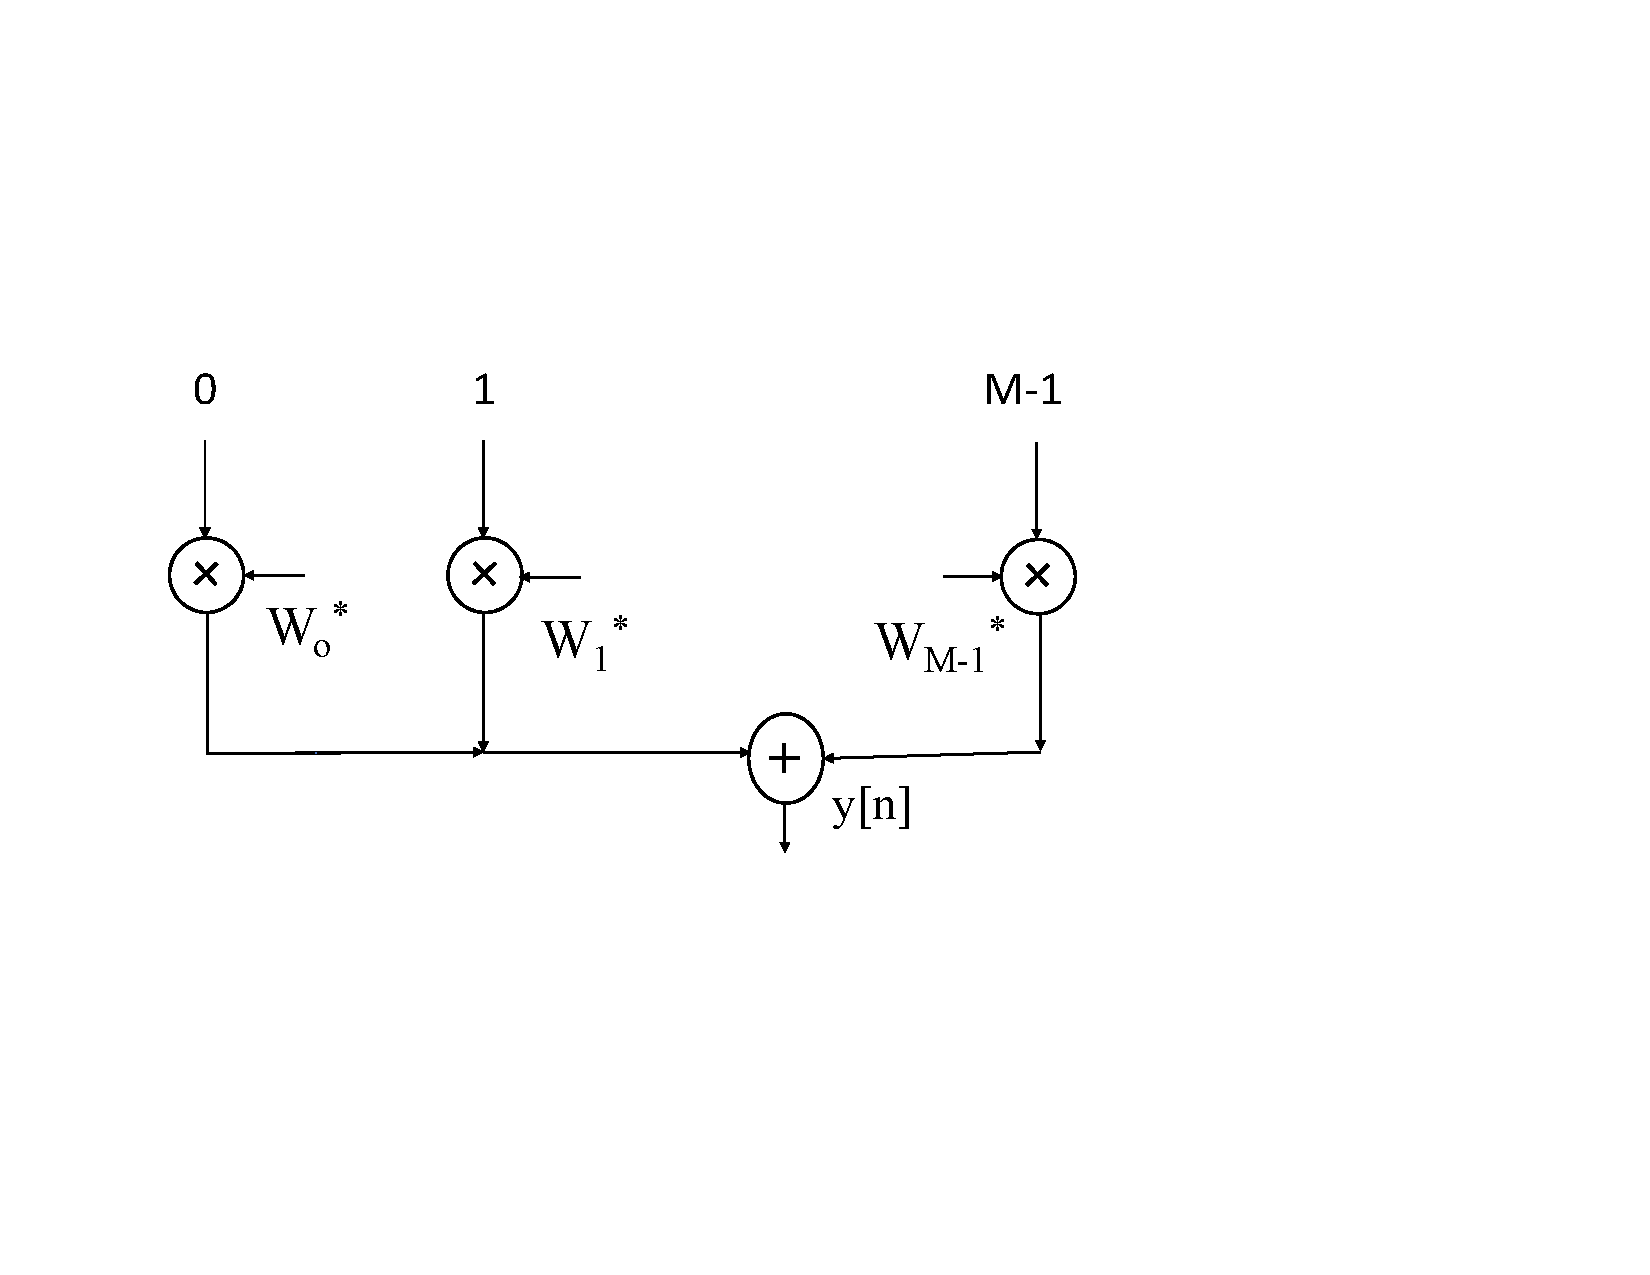
\includegraphics[scale=0.55, trim=0cm 7cm 5cm 4cm, clip]{summe.pdf}
	\caption{Sensors, figure \ref{ula}}
	\label{summe} 
\end{figure}
\begin{doublespace}
$y[n]= \vec{w}^H \vec{u}[n]$\\
$y[n]^*= \vec{u}^H[n] \vec{w}$\\ \ \\
$y^*[n] = \begin{bmatrix}y^*[n]\\ y^*[n-1]\\ \svdots \\ y^*[n+N]\end{bmatrix} = \underbrace{\begin{bmatrix}\vec{u}^H[n]\\ \vec{u}^H[n+1]\\ \svdots\\ \vec{u}^H[n+N]\end{bmatrix}}_{\ma{U}^H[n]}\vec{w}= \ma{U}^H[n]\vec{w}$\\ \\
$\vec{u}[n]= \underbrace{\vec{a}(\Theta) s[n]}_{desired signal}+ \underbrace{\vec{\eta}[n]}_{\text{interference + noise}}$\\ \\
Constraint: $\vec{w}^H \vec{a}(\Theta)=1$\\
$y[n]=\vec{w}^H \vec{u}[n] = \vec{w}^H(\vec{a}(\Theta) s[n]+ \vec{\eta}[n])= \underbrace{\vec{w}^H\vec{a}(\Theta)}_1s[n]+ \vec{w}^H\vec{\eta}[n]= s[n] + \vec{w}^H\vec{\eta}[n]$\\\\
$\underset{\vec{w}}{min} \quad ||y[n]||_F^2$ \quad such that $\vec{w}^H \vec{a}(\Theta)=1$\\
\begin{tabular}{ll}
$||y[n]||_2^2$ &$= \vec{y}^H[n]\vec{y}[n]$\\
 &$=(\vec{y}^*[n])^H(\vec{y}[n]) \in \mathbb{R}$\\
 &$= (\ma{U}^H[n]\vec{w})^H(\ma{U}^H[n]\vec{w})$\\
 &$= \vec{w} \underbrace{\ma{U}[n]\ma{U}^H[n]}_{\ma{R}}{\vec{w}}= \vec{w}^H\ma{R}\vec{w}$\\
\end{tabular}
\end{doublespace}
\mybox{$\vec{w}_{OPT}= arg \min\limits_{\vec{w}} \vec{w}^H\ma{R}\vec{w}$, \qquad s.t. \quad $\vec{w}^H\vec{a}(\Theta)=1$}


\newpage
% SECTION ====================================================================================
\section{Mathematical background}
% ============================================================================================
\subsection{Gernral}
\subsubsection{Matrix inverse}
$\begin{bmatrix}a_{11}&a_{12}\\a_{21}&a_{22}\end{bmatrix}^{-1}=
\frac{1}{a_{11}a_{22}-a_{12}a_{21}}\begin{bmatrix}a_{22}&-a_{12}\\-a_{21}&a_{11}\end{bmatrix}$
\subsubsection{Hermitian matrix}
$\begin{bmatrix}a_{11}&a_{12}\\a_{21}&a_{22}\end{bmatrix}^{H}=
\begin{bmatrix}a_{11}^*&a_{21}^*\\a_{12}^*&a_{22}^*\end{bmatrix}$

\subsubsection{Quadratic equation}
$ax^2+bx+c=0\pfeil x_{1/2}=\frac{-b\pm\sqrt{b^2-4ac}}{2a}$\\
$x^2 + px + q=0 \pfeil x_{1/2}=-\frac{p}{2} \pm \sqrt{\frac{p^2}{4}-q} $\\

\subsubsection{Euklidian Norm}
$||\vec{v}||_2=\sqrt{v_1^2 + v_2^2 + ... + v_N} = \sqrt{\sum_{i=1}^{N}|v_i|^2}$
\subsubsection{Frobenius Norm}
$||\ma{V}||_F=\sqrt{|v_{1,1}|^2 + |v_{1,2}|^2+... + |v_{N,M}|^2} =\sqrt{\sum_{i=1}^{N} \sum_{j=1}^{M}|v_{i,j}|^2}$
\subsubsection{Taylor series}
$T f(x, a)  = \sum_{n=0}^\infty  \frac{f^{(n)}(a)}{n!} (x-a)^n = f(a) + f'(a) (x-a) + \frac{f''(a)}{2}(x-a)^2 + \frac{f'''(a)}{6} (x-a)^3 + \ldots$
\subsubsection{Fourier series}
$f(t)=\frac{a_{0}}{2}+\sum_{k=1}^{\infty}\left(a_{k}\cos\left(kt\right)+b_{k}\sin\left(kt\right)\right)$\\
$a_{k}=c_{k}+c_{-k}\quad\text{für }k\geq0$\\
$b_{k}=\mathrm{i}\left(c_{k}-c_{-k}\right)\quad\text{für }k\geq1$\\
or as an alternative:\\
$a_{k} = \frac{1}{\pi}\int_{-\pi}^{\pi}f(t)\cdot\cos\left(kt\right)\mathrm dt\quad\text{für }k\geq0$\\
$b_{k} = \frac{1}{\pi}\int_{-\pi}^{\pi}f(t)\cdot\sin\left(kt\right)\mathrm dt\quad\text{für }k\geq1$

\subsection{Complex derivative }
\subsubsection{Analytic function}
\begin{doublespace}
	

$ h: \mathbb{C} \ni z \mapsto h(z) \in \mathbb{C} \quad\, \with z=x +\j y \quad x,y\in\mathbb{R}$


$\frac{dh}{dz}=\lim\limits_{\Delta z \to 0}\frac{h(z+\Delta z)-h(z)}{\Delta z}$

$h(z)=h(x +\j y)=f(x,y) \quad  f: \mathbb{R}^2 \ni (x,y) \mapsto f(x,y) \in \mathbb{C} $

$dh=df=\frac{\partial f}{\partial x}dx+\frac{\partial f}{\partial y}dy$

$\quad$Substitution:  $ dx=a\cdot dt,\quad dy=b\cdot dt,\quad (a,b)\in\mathbb{R}^2 \backslash (0,0)$


$dz=dx+\j dy=(a+jb)dt\pfeil dx=\frac{a}{a+\j b}dz,\quad dy=\frac{b}{a+\j b}dz$ \ \\

$df=dh=\underbrace{\frac{\frac{\partial f}{\partial x}a+\frac{\partial f}{\partial y}b}{a+\j b}}_{H(z)} dz$
\end{doublespace}
\mybox{\begin{itemize}
\item Definition: $h(z)$ is analytic if and only if (iff) $H(z)$ exist and is independent of $(a,b)\in\mathbb{R}^2 \backslash (0,0)$
\item if $h(z)$ is analytic then $\frac{dh}{dz}=H$
\end{itemize}
$\frac{\partial H}{\partial a}=\frac{\j b}{(a+\j b)^2} \underbrace{\left(\frac{\partial f}{\partial x}+\j \frac{\partial f}{\partial y}\right)}_{=0},\qquad 
\frac{\partial H}{\partial b}=\frac{-\j a}{(a+\j b)^2} \underbrace{\left(\frac{\partial f}{\partial x}+\j \frac{\partial f}{\partial y}\right)}_{=0}$
\begin{itemize}
\item $h(z)$ is analytic if and only if $\frac{df}{dx}$ and $\frac{df}{dy}$ exist and $\frac{df}{dx} + \j \frac{df}{dy}=0$.
\item if $h(z)$ is analytic then $\frac{dh}{dz}=\frac{df}{dx} = - \j \frac{df}{dy}$
\end{itemize}}

\mybox{
\textbf{Example for analytic functions} - Exponential function

$h(z)=z^k \quad k\in \mathbb{R}$

$f(x,y)=(x+\j y)^k$

$\frac{df}{dx} + \j \frac{df}{dy}= k(x+\j y)^{k-1}+\j k(x+\j y)^{k-1} \j =0$, hence it is an analytic function 

Result: \quad $\frac{dh}{dz} = k(x+\j y)^{k-1}=k\cdot z^{k-1}$}

\textbf{other analytic functions}

\begin{itemize}
\item $h(z)=const.$
\item $h(z)=e^z$
\item $h(z)=\ln (z)$,  of $z=0$
\item $h(z)=\frac{\sum_{k=0}^\infty a_k \cdot z^k}{\sum_{k=0}^\infty b_k \cdot z^k}$,  for the poles
\end{itemize}

\textbf{example of non-analytic functions:}
\begin{itemize}
\item $h(z)=z^*=x-\j y=f(x,y)$

$\frac{\partial f}{\partial x}+\j \frac{\partial f}{\partial y}= 1 +\j (-\j) =2 \neq 0 \Rightarrow $ non analytic
\item $h(z)=\Re{z}=\frac{z+z^*}{2}$

$h:\mathbb{C}\ni z\mapsto h(z)\in\mathbb{R}$ is non-analytic,  it is a constant
\item $\vec{w}^H\ma{R}\vec{w}$
\end{itemize}



\subsubsection{Derivatives of non-analytic functions }



$\left. \begin{array}{l}z= x+jy, \quad\\z^*= x-jy\\ \end{array}\right\rbrace \quad x=\frac{z+z^*}{2},  y=\frac{z-z^*}{2j} \quad x,y \in \mathbb{R}$\\

$h(z)=h(x+\j y)=f(x,y)=f\left(\frac{z+z^*}{2},\frac{z-z^*}{\j 2}\right)=g(z,z^*)$

$df=\frac{\partial f}{\partial x}dx+\frac{\partial f}{\partial y}dy$

$dg=\frac{\partial g}{\partial z}dz+\frac{\partial g}{\partial z^*}dz^* =\frac{\partial g}{\partial z}(dx+\j dy)+\frac{\partial g}{\partial z^*}(dx-\j dy) $
$=\underbrace{\left(\frac{\partial g}{\partial z}+\frac{\partial g}{\partial z^*}\right)}_{\frac{\partial f}{\partial x}}dx
+\j \underbrace{\left(\frac{\partial g}{\partial z}-\frac{\partial g}{\partial z^*}\right)}_{\frac{\partial f}{\partial y}}dy$

In matrix notation\ 
\begin{doublespace}


\quad $  	\begin{bmatrix} \frac{\partial f}{\partial x} \\
	 \frac{\partial f}{\partial y}\end{bmatrix} =
    	\begin{bmatrix}  1 & 1 \\  \j & -\j  \end{bmatrix}
    \begin{bmatrix}  \frac{\partial g}{\partial z} \\
     \frac{\partial g}{\partial z^*} \end{bmatrix}$\ \\ \ \\
     
\quad $  	\begin{bmatrix} \frac{\partial g}{\partial z} \\
	 \frac{\partial g}{\partial z^*}\end{bmatrix} =
    	\frac{1}{2}\begin{bmatrix}  1 & -\j \\  1 & \j  \end{bmatrix}
    \begin{bmatrix}  \frac{\partial f}{\partial x} \\
     \frac{\partial f}{\partial y} \end{bmatrix}$ \ \\
\end{doublespace}
Note: $\frac{\partial g}{\partial z^*} = \frac{1}{2}\frac{\partial f}{\partial x} +\frac{1}{2} \j\frac{\partial f}{\partial y}$

$g(z,z^*)=h(z)$ is analytic iff $\frac{\partial g}{\partial z^*}=0$

$(\frac{\partial g}{\partial z^*})^*=\frac{\partial g^*}{\partial z}\neq \frac{\partial g}{\partial z}$  

 when $g: \mathbb{C}^2 \mapsto \mathbb{R}$ then: $(\frac{\partial g}{\partial z^*})^*= \frac{\partial g}{\partial z}$

\textbf{In the following, we assume that}

$h:\mathbb{C}\mapsto\mathbb{R},\quad g:\mathbb{C}^2\mapsto\mathbb{R}$

$dg=\frac{\partial g}{\partial z}dz+\underbrace{\frac{\partial g}{\partial z^*}dz^*}_{\text{only if} \mapsto \mathbb{R}: (\frac{\partial g}{\partial z}dz)^*} = 2\Re{\frac{\partial g}{\partial z}dz}$

\textbf{Local extrema}
$dg = 0 \quad \forall dz   \qquad \iff \qquad \frac{\partial g}{\partial z}=0$

\textbf{multiple variables}

$g:\mathbb{C}^{2n}\mapsto \mathbb{R}; \qquad g(z_1,z_2,...,z_n,z_1^*,z_2^*,...,z_n^*)=g(\vec{z},\vec{z}^*)$

$dg=\sum_{k=1}^{n} \frac{\partial g}{\partial z_k}dz_k+\sum_{k=1}^{n} \frac{\partial g}{\partial z_k^*}dz_k^* $
$=2\Re{\sum_{k=1}^{n}\frac{\partial g}{\partial z_k}dz_k}$



\subsubsection{Gradient vector}
$\frac{\partial}{\partial\vec{z}}=\begin{bmatrix}\partial/\partial z_1 \\ \partial/\partial z_2 \\ \svdots \\\partial/\partial z_n  \end{bmatrix} $ \qquad
$\frac{\partial}{\partial\vec{z}}g=\frac{\partial g}{\partial\vec{z}}=\begin{bmatrix}\partial g/\partial z_1 \\ \partial g/\partial z_2 \\ \svdots \\\partial g/\partial z_n  \end{bmatrix} $
$d\vec{z}=\begin{bmatrix}dz_1 \\ dz_2 \\ \svdots \\ dz_n\end{bmatrix}$ \ \\

Scalar product:

$\sum\limits_{k=1}^n \frac{\partial g}{\partial z_k}dz_k=\left(\frac{\partial g}{\partial \vec{z}}\right)^Td\vec{z}$\ \\

$dg=2\Re{\left(\frac{\partial g}{\partial \vec{z}}\right)^Td\vec{z}}=2\Re{\left(\left(\frac{\partial g}{\partial \underline{z^*}}\right)^*\right)^Td\vec{z}}$
$=2\Re{\left(\frac{\partial g}{\partial \underline{z^*}}\right)^Hd\vec{z}}$\ \\

\textbf{Local extrema}
$dg = 0 \quad \forall d\vec{z}   \qquad \iff \qquad \frac{\partial g}{\partial \vec{z}^*}=\underline{0}$

\textbf{Steepest descent}

\begin{doublespace}


$\vec{z}\rightarrow\vec{z}+\Delta\vec{z}$

$dg=2\Re{\left(\frac{\partial g}{\partial \underline{z^*}}\right)^H\Delta\vec{z}} \leq2 \left|\left( \frac{\partial g}{\partial \underline{z^*}}\right)^H\Delta\vec{z} \right|$

equality only if $\left(\frac{\partial g}{\partial \underline{z^*}}\right)^H\Delta\vec{z}\in \mathbb{R}_0^+ $

$\Delta \vec{z}=\varepsilon \frac{\partial g}{\partial \vec{z}^*} \Rightarrow  \left(\frac{\partial g}{\partial \underline{z^*}}\right)^H\Delta\vec{z} = \varepsilon \left(\frac{\partial g}{\partial \underline{z^*}}\right)^H\left(\frac{\partial g}{\partial \underline{z^*}}\right)\quad \in \mathbb{R}_0^+ \qquad \varepsilon > 0$

steepest descent: $\Delta \vec{z}= -\frac{\partial g}{\partial \vec{z}^*}$
\end{doublespace}
\textbf{Example 1}

$g=\vec{z}^H\vec{p}+\vec{p}^H\vec{z}; \quad \vec{p}=const$

g is real:

$g=g^*=g^H=(\vec{z}^H\vec{p}+\vec{p}^H\vec{z})^H=\vec{p}^H\vec{z}+\vec{z}^H\vec{p}=g $

$ g=g^* \Rightarrow real$

$\frac{\partial g}{\partial \vec{z}^*}=\frac{\partial}{\partial \vec{z}^*}(\vec{z}^H\vec{p}+\vec{p}^H\vec{z})=\frac{\partial}{\partial \vec{z}^*}(\vec{z}^H\vec{p})$
$=\frac{\partial}{\partial \vec{z}^*} \sum\limits_{k=1}^n z_k^* P_k =\begin{bmatrix}
\frac{\partial}{\partial z_1^*} \sum_{k=1}^n z_k^* P_k \\
\frac{\partial}{\partial z_2^*} \sum_{k=1}^n z_k^* P_k \\
\svdots\\
\frac{\partial}{\partial z_n^*} \sum_{k=1}^n z_k^* P_k 
\end{bmatrix} =\begin{bmatrix}P_1\\P_2\\ \svdots\\P_n\end{bmatrix} =\vec{p}$

result:  $ \frac{\partial}{\partial \vec{z}^*}(\vec{z}^H\vec{p}+\vec{p}^H\vec{z}) = \vec{p} $

alternative: $ \frac{\partial}{\partial \vec{z}}(\vec{z}^H\vec{p}+\vec{p}^H\vec{z}) = \vec{p}^* $

\textbf{Example 2}

$g=\vec{z}^H\ma{R}\vec{z}; \qquad \ma{R}=\ma{R}^H=const$

g is real:

$g^*=g^H=(\vec{z}^H\ma{R}\vec{z})^H=\vec{z}^H\ma{R}^H\vec{z} 
\overset{\ma{R}=\ma{R}^H}{=} 
g\Rightarrow real $

$\frac{\partial g}{\partial \vec{z}^*}
=\frac{\partial}{\partial \vec{z}^*}(\vec{z}^H\underbrace{\ma{R}\vec{z}}_{\vec{p}})
=\frac{\partial}{\partial \vec{z}^*}(\vec{z}^H\vec{p})
=\vec{p}
=\ma{R}\vec{z}$

$\vec{p}$ does not depend on $\vec{z}^*$

result: $\frac{\partial g}{\partial \vec{z}^*}=\frac{\partial}{\partial \vec{z}^*}(\vec{z}^H\ma{R}\vec{z})=\ma{R}\vec{z}$

\subsection{Minimization with linear equality constraints }

\subsubsection{Real-valued}
$\min\limits_{\vec{x}\in\mathbb{R}^n} \vec{x}^T\ma{R}\vec{x}, \qquad s.t.\quad  \vec{a}^T\vec{x}=b,  \quad \ma{R}\in\mathbb{R}^{nxn}, \vec{a}\in\mathbb{R}^n, b\in\mathbb{R}$ \ \\

Method of Lagrange 

$\mathcal{L}(\vec{x},\lambda):= \vec{x}^T\ma{R}\vec{x}+\lambda(\vec{a}^T\vec{x}-b)\quad \Rightarrow \quad \min\limits_{\vec{x}}\max\limits_{\lambda}\mathcal{L}(\vec{x},\lambda)$


\subsubsection{Complex-valued}
$\min\limits_{\vec{z}\in\mathbb{C}^n} \vec{z}^H\ma{R}\vec{z}, \qquad s.t.\quad  \vec{a}^H\vec{z}=b,  \quad \ma{R}\in\mathbb{C}^{nxn}, \vec{a}\in\mathbb{C}^n, b\in\mathbb{C}$\ \\ 

$\ma{R}=\ma{R}^H \in \mathbb{C} \quad \text{and} \quad\ma{R} \geq \vec{0}$\\

$ \mathcal{L}(\vec{z},\lambda_R,\lambda_I):= \vec{z}^H\ma{R}\vec{z}+\lambda_R\Re{\vec{a}^H\vec{z}-b}+\lambda_I\Im{\vec{a}^H\vec{z}-b}$

$ \mathcal{L}(\vec{z},\lambda):= \vec{z}^H\ma{R}\vec{z}+2\Re{\lambda^*(\vec{a}^H\vec{z}-b)}$

$\qquad =\vec{z}^H\ma{R}\vec{z}+\lambda^*(\vec{a}^H\vec{z}-b)+(\vec{z}^H\vec{a}-b^H)\lambda$

$\qquad =\mathcal{L}(\vec{z},\vec{z}^*,\lambda,\lambda^*)$


\subsubsection{Several complex constraints}
$\min\limits_{\vec{z}\in\mathbb{C}^n} \vec{z}^H\ma{R}\vec{z}, 
\qquad s.t.\quad 
\left\lbrace \begin{array}{l} \vec{a}_1^H\vec{z}=b_1\\ \svdots \\ \vec{a}_m^H\vec{z}=b_m \end{array} \right.$

$\mathcal{L}=\vec{z}^H\ma{R}\vec{z} + \sum\limits_{k=1}^m\lambda_k^*(\vec{a}_k^H\vec{z}-b_k)+\sum\limits_{k=1}^m(\vec{z}^H\vec{a}_k-b_k^*)\lambda_k$

with: 
\begin{itemize}
\item $\vec{\lambda}=\begin{bmatrix}\lambda_1\\\svdots\\\lambda_m\end{bmatrix}\in\mathbb{C}^m, \quad \vec{b}
=\begin{bmatrix}b_1\\\svdots\\b_m\end{bmatrix}\in\mathbb{C}^m$
\item $\sum\limits_{k=1}^m\lambda_k^*b_k=\vec{\lambda}^H\vec{b}$
\item $\sum\limits_{k=1}^m\lambda_k^*\vec{a}_k^H\vec{z}
=\vec{\lambda}^H\begin{bmatrix}\vec{a}_1^H  \vec{z}\\\svdots\\ \vec{a}_m^H  \vec{z} \end{bmatrix}
=\vec{\lambda}^H\begin{bmatrix}\vec{a}_1^H\\\svdots\\ \vec{a}_m^H  \end{bmatrix}\vec{z} 
=\vec{\lambda}^H\ma{A}^H\vec{z}$
\end{itemize}

follows:

$\min\limits_{\vec{z}\in\mathbb{C}^n} \vec{z}^H\ma{R}\vec{z}, 
\qquad s.t.\quad 
\ma{A}^H\vec{z}=\vec{b}, \quad \ma{R}=\ma{R}^H$

$\mathcal{L}=\vec{z}^H\ma{R}\vec{z}+\vec{\lambda}^H(\ma{A}^H\vec{z}-\vec{b})+(\vec{z}^H\ma{A}-\vec{b}^H)\vec{\lambda}
$

$\Rightarrow \quad \min\limits_{\vec{z}}\max\limits_{\vec{\lambda}}\mathcal{L}(\vec{x},\lambda)$

\mybox{
\textbf{Solution}

$\ma{R}$ is positive definite: $\ma{R}=\ma{R}^H \iff \ma{R}^{-1}$ exists and $\ma{R}^{-1}=(\ma{R}^{-1})^H $

$\frac{\partial L}{\partial \vec{z}^*}=\ma{R}\vec{z}+\ma{A}\vec{\lambda} \overset{!}{=} \vec{0}
\quad \Rightarrow \vec{z}=-\ma{R}^{-1}\ma{A}\vec{\lambda}$

$\vec{b}=\ma{A}^H\vec{z}=-\ma{A}^H\ma{R}^{-1}\ma{A}\vec{\lambda}
 \quad \Rightarrow \vec{\lambda}=-(\ma{A}^H\ma{R}^{-1}\ma{A})^{-1}\vec{b}$

$\mathbf{\vec{z}_{opt}=\ma{R}^{-1}\ma{A}(\ma{A}^H\ma{R}^{-1}\ma{A})^{-1}\vec{b}}$}

check if local minimum

$\Delta\vec{z}$ such that $\ma{A}^H(\vec{z}_{opt}+\Delta\vec{z})=\vec{b}   
\quad \iff \ma{A}^H\Delta\vec{z} =\vec{0}$ \qquad $\Delta \vec{z}\in \operatorname{null} \ma{A}$; see section \ref{sssec:svd}

$d\mathcal{L}=2\Re{\frac{\partial L}{\partial \vec{z}^*}d\vec{z}}$

$\frac{\partial \mathcal{L}}{\partial \vec{z}^*}=\ma{R}\vec{z}+\ma{A}\vec{\lambda}
=\ma{R}(\vec{z}_{opt}+\Delta \vec{z})+\ma{A}\vec{\lambda}$
$=\underbrace{\ma{R}\vec{z}_{opt}+\ma{A}\vec{\lambda}}_{\vec{0}}+\ma{R}\Delta\vec{z}
=\ma{R}\Delta\vec{z}$

$d\mathcal{L}=2\Re{\Delta \vec{z}^H\ma{R}^H(-\Delta \vec{z})}
=-2\Re{\underbrace{\Delta \vec{z}^H\ma{R}^H\Delta\vec{z}}_{>0}}=-2\underbrace{\Delta\vec{z}^H\ma{R}\Delta\vec{z}}_{>0}<0$ \quad local minimum

$\mathcal{L}=\vec{z}^H\ma{R}\vec{z}+\vec{\lambda}^H(\ma{A}^H\vec{z}-\vec{b})+(\vec{z}^H\ma{A}-\vec{b}^H)\vec{\lambda}$ \quad if constraints met: $\mathcal{L}=\vec{z}^H\ma{R}\vec{z}$
\newpage
\subsection{Linear Algebra}
\subsubsection{Vector spaces}
\mybox{
\textbf{Definition:} A \textbf{vector space} $\mathbb{V}$ over a set $\mathbb{K}$ is a set such that: 
\begin{enumerate}
\item $\forall \vec{a},\vec{b}\in\mathbb{V}: \qquad \vec{a}+\vec{b}\in\mathbb{V}$\\
The vectors $\vec{a}$ and $\vec{b}$ in vectorspace  $\mathbb{V}$ can be added to a new vector in the vector space.
\item $\forall \vec{a},\vec{b}\in\mathbb{V}: \qquad \vec{a}+\vec{b}=\vec{b}+\vec{a}$\\
Addition in commutative.
\item $\forall \vec{a},\vec{b},\vec{c}\in\mathbb{V}: \quad (\vec{a}+\vec{b})+\vec{c}=\vec{a}+(\vec{b}+\vec{c})$\\
The order to operate addition ist not relevant.
\item $\forall \vec{a}\in\mathbb{V}: \exists \vec{0} \in \mathbb{V}: \vec{a} + \vec{0}= \vec{a} $ with $\vec{0} $ as the identity element.\\
The sum of a vector with the zero-vector equals the original vector.
\item $\forall \vec{a} \in \mathbb{V}: \exists - \vec{a} \in \mathbb{V}: \vec{a} + (-\vec{a})= \vec{0} $\\
The sum of a vector with it's negative opponent equals the zero-vector.
\item $\forall \vec{a} \in \mathbb{V}: 1\vec{a}=\vec{a} ; 1 \in  \mathbb{K} $\\
Scaling a vector with 1 results in the vector.
\item $\forall \vec{a} \in \mathbb{V}, \forall \lambda, \mu \in  \mathbb{K}: \lambda (\mu \vec{a}) = (\lambda \mu)\vec{a}$\\
Scaling a vector with two scalars is commutative.
\item $\forall \vec{a}, \vec{b}\in \mathbb{V}, \forall \lambda \in  \mathbb{K}: \lambda (\vec{a}+ \vec{b})= \lambda \vec{a} + \lambda \vec{b}$\\
Scaling two vectors with the same scalar equals scaling two vectors with the scalar seperately.
\item $\forall \vec{a} \in \mathbb{V}, \forall \lambda, \mu \in  \mathbb{K}: (\mu + \lambda)\vec{a}= \mu\vec{a}+\lambda \vec{a}$\\
It's irrelevant if two scalars are summed up first or multiplied by a vector individually.
\end{enumerate}}


\textbf{Conclusion:}
\begin{enumerate}
\item $\vec{a}+\vec{a}=2\vec{a} \quad \mathbb{K}=\mathbb{C}$

proof:	$\overbrace{\vec{a}+\vec{a}}^{\textcirc{1}}  \overset{\textcirc{6}}{=} 1\vec{a}+1\vec{a} \overset{\textcirc{9}}{=} \overbrace{(1+1)}^{2 in\mathbb{K}}\vec{a}=2\vec{a}$
\item $\vec{0}$ is unique 


proof: Assume there is another $\vec{0}$

$\left. \begin{array}{l}
\textcirc{4}\quad \vec{0}'+\vec{0}= \vec{0}'\\
\textcirc{4}\quad \vec{0}+\vec{0}'= \vec{0}\\
\textcirc{2}\quad \vec{0}'+\vec{0}=\vec{0}+\vec{0}'
\end{array} \right\rbrace
\vec{0}'=\vec{0}$
\end{enumerate}

\textbf{Example of vector spaces}

\begin{itemize}
\item $\left\lbrace\vec{0}\right\rbrace$ 
\item $\mathbb{K}=\mathbb{Z}, \mathbb{V}=\mathbb{Z}$ \quad integer numbers
\item $\mathbb{K}=\mathbb{C}, \mathbb{V}=\mathbb{C}$ \quad complex numbers
\item $\mathbb{K}=\mathbb{C},$

$\mathbb{V}=\left\lbrace a_0+a_1z+a_2z^2+ \shdots +a_nz^n |z,a_0,\shdots,a_n \in \mathbb{C} \right\rbrace$ \quad polynoms
\item $\mathbb{K}=\mathbb{C}, \mathbb{V}=\mathbb{C}^n=\left\lbrace \begin{bmatrix}
a_1 \\ \svdots \\ a_n
\end{bmatrix} \right\rbrace, a_1,a_2,\shdots,a_n \in \mathbb{C}$ \quad vectors 
\end{itemize}

\textbf{counter example}

\begin{itemize}
\item $\left\lbrace \right\rbrace$ \quad empty set
\end{itemize}

\mybox{
\textbf{Definition:} A set $\mathbb{S}$ is called \textbf{subspace of a vector space} $\mathbb{V}$ over $\mathbb{K}$, if and only if:

\begin{enumerate}
\item $\mathbb{S}\subseteq \mathbb{V}$ \qquad Must be a subset of $\mathbb{V}$
\item $\forall \vec{a},\vec{b}\in\mathbb{S}: \vec{a}+\vec{b}\in\mathbb{S}$
\item $\forall\vec{a}\in\mathbb{S},\forall\lambda\in\mathbb{K}: \lambda\vec{a}\in\mathbb{S}$
\end{enumerate}}
Note: $\vec{0}\in\mathbb{S}; \mathbb{S}\neq\left\lbrace\right\rbrace$

Linear combination: $\vec{v}_1, ... , \vec{v}_n\in\mathbb{S}\Rightarrow \sum\limits_{k=1}^{n}a_k\vec{v}_k \in \mathbb{S}; a_k\in\mathbb{K}$


\subsubsection{Vectors}
\begin{doublespace}


In the following 

$\mathbb{K}=\mathbb{C}, \mathbb{V}=\mathbb{C}^m$

$a_1,...,a_m\in\mathbb{C}$

colum vector: $\vec{a}:=\begin{bmatrix}a_1\\\svdots\\a_m\end{bmatrix} $

row vector: $\vec{a}^T:=\begin{bmatrix}a_1&\shdots&a_m\end{bmatrix} \quad (\vec{a}^T)^T=\vec{a}$

complex conjugate: $\vec{a}^*=\begin{bmatrix}a_1^*\\\svdots\\a_m^*\end{bmatrix}\quad (\vec{a}^*)^*=\vec{a}$

Hermite-ian vector: $(\vec{a}^*)^T=(\vec{a}^T)^*:= \vec{a}^H \quad (\vec{a}^H)^H=\vec{a}$

complex scalar product: $\vec{a}^H\vec{b}=a_1^*b_1+...+a_m^*b_m=(\vec{b}^H\vec{a})^*$

$\vec{a},\vec{b}$ are orthogonal iff $\vec{a}^H\vec{b}=\vec{b}^H\vec{a}=0$

euclidian norm: $\left|\left|\vec{a}\right|\right|_2:=\sqrt{\vec{a}^H\vec{a}}=\sqrt{a_1^*a_1+...+a_m^*a_m}=\sqrt{\left|a_1\right|^2+...+\left|a_m\right|^2}$

\mybox{\textbf{Definition: Span}  

$\Sp(\vec{v}_1,...,\vec{v}_n):=\left\lbrace \sum\limits_{k=1}^n a_k\vec{v}_k | a_1,...,a_n\in\mathbb{C} \right\rbrace$

$ \vec{v}_1,...,\vec{v}_n\in\mathbb{C}^m$

Note: $\Sp(\vec{v}_1,...\vec{v}_n)$ is a subspace of $\mathbb{C}^m$}

\mybox{\textbf{Definition:} 

The vectors $\vec{v}_1,...\vec{v}_n$ are linearly independent (LID) if and only if: $a_1\vec{v}_1+a_2\vec{v}_2...+a_n\vec{v}_n=\vec{0}$ requires that $a_1=...=a_n=0$ 

\textbf{Theorem:} 

if $\vec{v}_1,...\vec{v}_n$ are not LID, that is if they are linearly dependent (LD), then $\exists_i:\vec{v}_i=\sum\limits_{k=1,k\neq i}^n b_k\vec{v}_k$ and vice versa (und umgekehrt)}

\textbf{Proof:}

$a_1\vec{v}_1+...+a_n\vec{v}_n=\vec{0}$ for $\vec{v}_i$ with $a_i\neq 0$

$\quad a_k=\left\lbrace \begin{array}{l}b_k \textrm{ for } k\neq i\\-1 \textrm{ for } k=1\end{array}\right.$ \qed

\mybox{\textbf{Definition:}

Dimension, $dim\mathbb{S}$ of a subset $\mathbb{S}$ is the maximum number of LID vectors in $\mathbb{S}$
}

\mybox{
\textbf{Theorem:}

Every subset $\mathbb{S}$ with $dim\mathbb{S}=n$ is a span $\Sp(\vec{v}_1,...,\vec{v}_n)$ of n LID vectors $\vec{v}_1,...,\vec{v}_n$ in $\mathbb{S}$}
\end{doublespace}
\textbf{Proof:}

\begin{itemize}
\item $\Sp(\vec{v}_1,...,\vec{v}_n)\subseteq \mathbb{S}$, from definition
\item show $\mathbb{S}\subseteq \Sp(\vec{v}_1,...,\vec{v}_n)$ 
\end{itemize}
\begin{doublespace}
	suppose $\vec{s}\in\mathbb{S}: \vec{s}\in \Sp(\vec{v}_1,...,\vec{v}_n)$, then $(\vec{v}_1,...,\vec{v}_n,\vec{s})$ are LID 

$\underbrace{(\vec{v}_1,...,\vec{v}_n,\vec{s})}_{dim=n+1}\subseteq \underbrace{\mathbb{S}}_{dim =n}$ because $\vec{s}\in\mathbb{S}$

$\Rightarrow \forall \vec{s}\in\mathbb{S}: \vec{s}\in \Sp(\vec{v}_1,...,\vec{v}_n))$

$\Rightarrow \mathbb{S}= \Sp(\vec{v}_1,...,\vec{v}_n)$\qed

\textbf{Note:} $dim(\vec{v}_1,...,\vec{v}_n)=n $ if $\vec{v}_1,...,\vec{v}_n$ are LID

\mybox{\textbf{Definition:} the n LID vectors $\vec{v}_1,...,\vec{v}_n$ are called \textbf{base vectors} of $\Sp(\vec{v}_1,...,\vec{v}_n)$}

\textbf{Note:} base vectors are not unique: 

eg: $\mathbb{S}_1=\Sp\left(\begin{bmatrix}0\\1\\0\end{bmatrix},\begin{bmatrix}0\\1\\1\end{bmatrix}\right)$ ,
$\mathbb{S}_2=\Sp\left(\begin{bmatrix}0\\2\\1\end{bmatrix},\begin{bmatrix}0\\0\\-1\end{bmatrix}\right)$


$\begin{bmatrix}0\\2\\1\end{bmatrix}=\begin{bmatrix}0\\1\\0\end{bmatrix}+\begin{bmatrix}0\\1\\1\end{bmatrix}, 
\begin{bmatrix}0\\0\\-1\end{bmatrix}=\begin{bmatrix}0\\1\\0\end{bmatrix}-\begin{bmatrix}0\\1\\1\end{bmatrix} 
\Rightarrow \mathbb{S}_1 \subseteq \mathbb{S}_2 \textcirc{1}$\\ \ \\

$\begin{bmatrix}0\\1\\0\end{bmatrix}=\frac{1}{2}\!\begin{bmatrix}0\\2\\1\end{bmatrix}+\frac{1}{2}\!\begin{bmatrix}0\\0\\-1\end{bmatrix},
\begin{bmatrix}0\\1\\1\end{bmatrix}=\frac{1}{2}\!\begin{bmatrix}0\\2\\1\end{bmatrix}-\frac{1}{2}\!\begin{bmatrix}0\\0\\-1\end{bmatrix} 
\Rightarrow \mathbb{S}_2 \subseteq \mathbb{S}_1 \textcirc{2}$\\

$\textcirc{1} \& \textcirc{2} \Rightarrow \mathbb{S}_1=\mathbb{S}_2$\\

\mybox{\textbf{Definition:} Orthonormal base vectors $\vec{w}_1,...,\vec{2}_n$ have the property: 

$\vec{w}_j^H\vec{w}_k=\left\lbrace \begin{matrix}1,& i=k\\0,&else\end{matrix} \right.$}

\mybox{
\textbf{Theroem:} orthonormal vectors are LID}

\textbf{Proof:} $a_1\vec{w}_1+a_2\vec{w}_2+...+a_n\vec{w}_n=\vec{0}\quad |\vec{w}_1^H\cdot$

$a_1\underbrace{\vec{w}_1^H\vec{w}_1}_{1}+a_2\underbrace{\vec{w}_1^H\vec{w}_2}_{0}+...+a_n\underbrace{\vec{w}_1^H\vec{w}_n}_{0}=\underbrace{\vec{w}_1^H\vec{0}}_{0}\Rightarrow a_1=0$
\end{doublespace}
Repeat: $\begin{array}{l}\vec{w}_2^H:a_2=0\quad ...\quad\vec{w}_n^H:a_n=0\end{array}$\qed\\

\mybox{\textbf{Theorem:} Let $\vec{v}_1,...,\vec{v}_n\in\mathbb{C}^n$ be n LID vectors of $\mathbb{C}^n$, then $\Sp(\vec{v}_1,...,\vec{v}_n)=\Sp(\vec{e}_1,...,\vec{e}_n)\in\mathbb{C}^n$

with: $\vec{e}_1=\begin{bmatrix}1\\0\\0\\\svdots\end{bmatrix},\vec{e}_2=\begin{bmatrix}0\\1\\0\\\svdots\end{bmatrix},...,\vec{e}_n=\begin{bmatrix}0\\\svdots\\0\\1\end{bmatrix} \in\mathbb{C}^n$}

\textbf{Proof:} $\vec{v}_i=\sum\limits_{j=1}^na_{ji}\vec{e}_j\Rightarrow \Sp(\vec{v}_1,...,\vec{v}_n)\subseteq \mathbb{C}^n$

if $\exists\vec{s}\in\mathbb{C}^n: \vec{s}\in \Sp(\vec{v}_1,...,\vec{v}_n)$ then $(\vec{v}_1,...,\vec{v}_n,\vec{s})$ is LID
$\underbrace{\Sp(\vec{v}_1,...,\vec{v}_n,\vec{s})}_{dim=n+1}\subseteq\underbrace{\mathbb{C}^n}_{dim=n (wrong)}$ \qed

\mybox{\textbf{Theorem:} Every subspace has got orthonormal base-vectors
}
\textbf{Proof:} $\mathbb{S}=\Sp(\vec{v}_1,...,\vec{v}_n)$ with $\vec{v}_i$ is LID

Orthogonal vectors:

$\vec{u}_1=\vec{v}_1$\\

$\vec{u}_2=\vec{v}_2-\frac{\vec{u}_1^H\vec{v}_2}{\vec{u}_1^H\vec{u}_1}\vec{u}_1 $\\

$\vec{u}_1^H \vec{u}_2 = \vec{u}_1^H \vec{v}_2 - \vec{u}_1^H \vec{v}_2 = 0 \quad \vec{u}_2^H \vec{u}_1 = 0$\\

$\vec{u}_3=\vec{v}_3-\frac{\vec{u}_1^H\vec{v}_3}{\vec{u}_1^H\vec{u}_1}\vec{u}_1-\frac{\vec{u}_2^H\vec{v}_3}{\vec{u}_2^H\vec{u}_2}\vec{u}_2 $\\

$\vec{u}_k=\vec{v}_k-\sum\limits_{m=1}^{k-1}\frac{\vec{u}_m^H\vec{v}_k}{\vec{u}_m^H\vec{u}_m}\vec{u_m}, \with 2\leq k\leq n$\\

normalized vectors $\rightarrow$ orthonormal vectors:

$\vec{w}_i=\frac{\vec{u}_i}{\sqrt{\vec{u}_i^H\vec{u}_i}}$ \\
$\Rightarrow \vec{w}_i^H\vec{w}_k=\left\lbrace \begin{matrix}0,&i\neq k\\1,&i=k\end{matrix}  \right.$\\

$\Sp(\vec{w}_1,...,\vec{w}_n)=\Sp(\vec{v}_1,...,\vec{v}_n)$\qed\\ 
%}


\subsubsection{Matrices}
$\ma{A}=\begin{bmatrix}A_{11}&\shdots&A_{1n}\\\svdots& &\svdots\\A_{m1} & \shdots& A_{mn}\end{bmatrix}\in\mathbb{C}^{m\times n}$ \with m rows and n columns

$A_{ij}=(\ma{A})_{ij}$ element of $\ma{A}$ at the i-th row and j-th column 

$\ma{A}^*=\begin{bmatrix}A_{11}^*&\shdots&A_{1n}^*\\\svdots& &\svdots\\A_{m1}^* & \shdots& A_{mn}^*\end{bmatrix} \in \mathbb{C}^{m\times n}$
 
$\ma{A}^T=\begin{bmatrix}A_{11}&\shdots&A_{m1}\\\svdots& &\svdots\\A_{1n} & \shdots& A_{mn}\end{bmatrix} \in \mathbb{C}^{n\times m}$

Hermite-ian matrix: $(\ma{A}^*)^T=(\ma{A}^T)^*=\ma{A}^H$

Frobenius norm: $\left|\left| \ma{A}\right|\right|_F := \sqrt{\sum\limits_{k=1}^m\sum\limits_{p=1}^n \left|A_{kp}\right|^2}$

Zero matrix: $\ma{0}_{m\times n}=\begin{bmatrix}0&\shdots&0\\\svdots&&\svdots\\0&\shdots&0\end{bmatrix}\in \mathbb{C}^{m\times n},\quad \ma{0}_m \overset{!}{=}\ma{0}_{m\times m}$

Identity matrix: $\ma{I}_m=\begin{bmatrix}1&0&\shdots\\0&1& \\\svdots& &\ddots\end{bmatrix}$

Matrix multiplication: $\ma{C}=\ma{A}\ma{B} \iff C_{ik}=\sum\limits_{t}A_{it}\cdot B_{tk}$

$\underbrace{\begin{bmatrix}\vec{a}_1&\shdots&\vec{a}_p\end{bmatrix}}_{\ma{A}}
\underbrace{\begin{bmatrix}\vec{\beta}_1^H\\\svdots\\\vec{\beta}_p^H\end{bmatrix}}_{\ma{B}}=
\vec{a}_1\vec{\beta}_1^H+...+\vec{a}_p\vec{\beta}_p^H=\ma{C}$

$\underbrace{\begin{bmatrix}\vec{\alpha}_1^H\\\svdots\\\vec{\alpha}_m^H\end{bmatrix}}_{\ma{A}}
\underbrace{\begin{bmatrix}\vec{b}_1&\shdots&\vec{b}_n\end{bmatrix}}_{\ma{B}} =
\begin{bmatrix}\vec{\alpha}_1^H\vec{b}_1&\shdots&\vec{\alpha}_1^H\vec{b}_n\\
\svdots& &\svdots\\
\vec{\alpha}_m^H\vec{b}_1&\shdots&\vec{\alpha}_m^H\vec{b}_n\end{bmatrix}=\ma{C}$

Multiplication with sub matrices:

$\begin{bmatrix}\ma{A}&\ma{C}\\\ma{B}&\ma{D}\end{bmatrix}
\begin{bmatrix}\ma{E}&\ma{G}\\\ma{F}&\ma{H}\end{bmatrix}=
\begin{bmatrix}\ma{A}\ma{E}+\ma{C}\ma{F}&\ma{A}\ma{G}+\ma{C}\ma{H}\\\ma{B}\ma{E}+\ma{D}\ma{F}&\ma{B}\ma{G}+\ma{D}\ma{H}\end{bmatrix}$

example:

$\ma{M}=\begin{bmatrix}\ma{I}_m&\ma{F}\end{bmatrix}; \ma{Q}=\begin{bmatrix}-\ma{F}^H&\ma{I}_m\end{bmatrix}$

$\ma{M}\ma{Q}^H=\begin{bmatrix}\ma{I}_m&\ma{F}\end{bmatrix}\begin{bmatrix}-\ma{F}\\\ma{I}_m\end{bmatrix}
=\ma{I}_m(-\ma{F})+\ma{F}\ma{I}_m=\ma{F}-\ma{F}=\ma{0}$

\mybox{Identity matrix \\
$\ma{I} \ma{A} = \ma{A} \ma{I} = \ma{A}$\\
$\ma{A}^H(\ma{A}^H)^{-1} = \ma{I}$\\
If $\ma{B}\in\mathbb{C}^{m\times n}$ has $n$ orthonormal columns then $\ma{B}^H\ma{B}=\ma{I}$}\\

Multiplication with a vector:

$\ma{A}\vec{x}=\begin{bmatrix}\vec{a}_1&...&\vec{a}_n\end{bmatrix}\begin{bmatrix}x_1\\...\\x_n\end{bmatrix}
=\vec{a}_1x_1+...+\vec{a}_nx_n$

In general: $\ma{A}\ma{B}\neq\ma{B}\ma{A}$
\begin{itemize}
\item $(\ma{A}+\ma{B})^2=(\ma{A}+\ma{B})(\ma{A}+\ma{B})=\ma{A}^2+\ma{A}\ma{B}+\ma{B}\ma{A}+\ma{B}^2$
\item $(\ma{A}\ma{B})\ma{C}=\ma{A}(\ma{B}\ma{C})$
\item $(\ma{A}\ma{B})^T=\ma{B}^T\ma{A}^T$
\item $(\ma{A}\ma{B})^H=\ma{B}^H\ma{A}^H$
\end{itemize}

\mybox{\textbf{Definition: }Trace: 
$\tr\ma{A}=\sum\limits_{k}A_{kk}$}
\begin{itemize}
\item $\tr(\ma{A}\ma{B})=\tr(\ma{B}\ma{A})$
\item $\tr(\ma{A}\underbrace{\ma{B}\ma{C}}_{\ma{M}})=\tr(\ma{M}\ma{A})=\tr(\ma{B}\ma{C}\ma{A})$
\item $\tr(\ma{A}\ma{B}\ma{C})=\tr(\ma{B}\ma{C}\ma{A})=\tr(\ma{C}\ma{A}\ma{B})$
\item $\tr(\ma{A}\ma{A}^H)=\tr(\ma{A}^H\ma{A})$
\end{itemize}
$\tr(\ma{A}\ma{A}^H)=\tr(\ma{A}\ma{A}^H)=
\tr\begin{bmatrix}\vec{a}_1^H\\...\\\vec{a}_n^H\end{bmatrix}\begin{bmatrix}\vec{a}_1&...&\vec{a}_n\end{bmatrix}
=\tr\begin{bmatrix}\vec{a}_1^H\vec{a}_1 & & X\\ &\ddots& \\X& &\vec{a}_n^H\vec{a}_n\end{bmatrix}
=\sum\limits_{k=1}^n\vec{a}_k^H\vec{a}_k=\sum\limits_{k=1}^n||\vec{a}_k||^2_2
=\sum\limits_{k=1}^n\sum\limits_{p=1}^n|a_{kp}|^2=||\ma{A}||^2_F$

Frobenius norm: $\tr(\ma{A}^H\ma{A})=\tr(\ma{A}\ma{A}^H)=||\ma{A}||^2_F$

\mybox{\textbf{Definition:} $\ma{A}\in\mathbb{C}^{n\times n}$ is invertable if and only if: 

$\exists \ma{B}: \ma{A}\ma{B}=\ma{B}\ma{A}=\ma{I}_n$, then $\ma{B}=\ma{A}^{-1}$ is called inverse of $\ma{A}$}

\mybox{
\textbf{Theorem:} If $\ma{A}$ is invertable then $\ma{A}^{-1}$ is unique}

\textbf{Proof:} $\ma{C}$ is another inverse of $\ma{A}$

$\ma{C}=\ma{C}\ma{I}=\ma{C}\ma{A}\ma{B}=(\ma{C}\ma{A})\ma{B}=\ma{B}
\Rightarrow \ma{I}\ma{B}=\ma{B}=\ma{C}$ \qed

\mybox{\textbf{Theorem:} $(\ma{A}^H)^{-1}=(\ma{A}^{-1})^{H}=\ma{A}^{-H}$}

\textbf{Proof:} $\ma{A}\ma{A}^{-1}=\ma{I}\quad |(\cdot)^H$

$(\ma{A}\ma{A}^{-1})^H=(\ma{A}^{-1})^H\ma{A}^H=\ma{I}=(\ma{A}^H)^{-1}\ma{A}^H\quad|\cdot (\ma{A}^H)^{-1}$

$(\ma{A}^{-1})^H\underbrace{\ma{A}^H(\ma{A}^H)^{-1}}_{\ma{I}}
=(\ma{A}^H)^{-1}\underbrace{\ma{A}^H(\ma{A}^H)^{-1}}_{\ma{I}}$

$\Rightarrow(\ma{A}^{-1})^H=(\ma{A}^H)^{-1}$\qed

\mybox{\textbf{Theorem:} if $\ma{A}^{-1}$ exist, then columns of $\ma{A}$ are LID}

\textbf{Proof:} $\underbrace{\ma{A}\vec{x}=\vec{0}}_{\vec{a}_1x_1+...\vec{a}_nx_n=\vec{0}}
\Rightarrow \underbrace{\vec{x}=\ma{A}^{-1}\vec{0}=\vec{0}}_{x_1=x_2=...=x_n=0}$

$\Rightarrow \Sp(\vec{a}_1,...,\vec{a}_n)=\mathbb{C}^n$

$\exists \vec{b}_i: \ma{A}\vec{b}_i=\vec{e}_i \in \mathbb{C}^n$

$\Rightarrow \ma{A}\underbrace{\begin{bmatrix}\vec{b}_1,...,\vec{b}_n\end{bmatrix}}_{\ma{B}}=\begin{bmatrix}\vec{e}_1,...,\vec{e}_n\end{bmatrix}=\ma{I}$

$\exists \ma{B}: \ma{A}\ma{B}=\ma{I}$\qed


\subsubsection{Determinate}
$\det \ma{A}: \mathbb{C}^{n\times n}\mapsto \mathbb{C}$

Property 1: $n=1: \det A=A$

Property 2: If $\ma{A}$ has LD columns, then $\det A=0$

Property 3: $\det \ma{A}$ is linear in colums of $\ma{A}$

\quad \textcirc{1}: $\det [\vec{a}_1,...,\vec{a}_{i-1},\lambda\vec{a}_i,\vec{a}_{i+1},...,\vec{a}_n]=\lambda \det \ma{A}$

\quad \textcirc{2}: $\det [\vec{a}_1,...,\vec{a}_{i-1},\vec{a}_i,\vec{a}_{i+1},...,\vec{a}_n]$

\qquad\quad$+\det [\vec{a}_1,...,\vec{a}_{i-1},\vec{b}_i,\vec{a}_{i+1},...,\vec{a}_n]$

\qquad\quad$=\det [\vec{a}_1,...,\vec{a}_{i-1},\vec{a}_i+\vec{b}_i,\vec{a}_{i+1},...,\vec{a}_n]$

\mybox{
\textbf{Theorems:}

\begin{enumerate}
\item $\det \ma{A}$ is unique
\item $\det \ma{A}=\sum\limits_{i=1}^n(-1)^{i+j}A_{ij}\det \ma{A}^{(i,j)}$; for any j

\;  $\ma{A}^{(i,j)}\in\mathbb{C}^{(n-1)\times (n-1)}$:{\small  $\ma{A}$ with i-th row and j-th columns removed}
\item $\det \ma{I}_n=1$
\item $\det (\ma{A}\ma{B})=\det (\ma{A})\cdot \det (\ma{B})$
\item $\det (\ma{B}^{-1})=(\det \ma{B})^{-1}$
\item $\det \ma{A} = \det \ma{A}^T$ 
\end{enumerate}}

\begin{flushright}- without proof\end{flushright}

example:

\quad$\det a=a, a\in\mathbb{C}$

\quad $\det \begin{bmatrix}a&c\\b&d\end{bmatrix} = a\det(d)+(-1)b\det(c)=ad-bc$


\subsubsection{Eigenvalues}
\mybox{
\textbf{Definition:} $\lambda\in\mathbb{C}$ is an eigenvalue (Eval) of $\ma{A}\in\mathbb{C}^{n\times n}$ if $\exists\vec{b}\neq \vec{0}$ such that $(\ma{A}-\lambda\ma{I})\vec{b}=\vec{0}$, then $\vec{b}$ is a eigenvecotr (Evec) of $\ma{A}$ for the eigenvalue $\lambda$}

Properties: 
\begin{itemize}
\item \textbf{Eigenvalue} $\det(\ma{A}-\lambda\ma{I})=0$
\item $\ma{A}\vec{b}=\lambda\vec{b}$
\item given n LID eigenvectors $(\vec{b}_1,...,\vec{b}_n)$ of $\ma{A}\in\mathbb{C}^{n\times n}$ of the eigenvalues $(\lambda_1,...\lambda_n)$ then\\ $\ma{A}=\ma{B}\ma{\Lambda}\ma{B}^{-1}$ 
\item $\ma{B}=\begin{bmatrix}\vec{b}_1&...&\vec{b}_n\end{bmatrix}\in\mathbb{C}^{n\times n} $
\item $\ma{\Lambda}=\begin{bmatrix}\lambda_1& & \\ &\ddots & \\ & &\lambda_n\end{bmatrix} \in \mathbb{C}^{n\times n}$
\item $\ma{B}\ma{\Lambda}=\begin{bmatrix}\vec{b}_1&...&\vec{b}_n\end{bmatrix} 
\begin{bmatrix}\lambda_1& & \\ &\ddots & \\ & &\lambda_n\end{bmatrix}$

$=\begin{bmatrix}\underbrace{\vec{b}_1\lambda_1}_{\ma{A}\vec{b}_1}&...&\underbrace{\vec{b}_n\lambda_n}_{\ma{A}\vec{b}_n}\end{bmatrix}=\ma{A}\begin{bmatrix}\vec{b}_1&...&\vec{b}_n\end{bmatrix}=\ma{A}\ma{B}$
\item \textbf{Eigenvalue Decomposition, EVD}: $\ma{A}=\ma{B}\ma{\Lambda}\ma{B}^{-1}$
\end{itemize}

\mybox{
\textbf{Note:}
\begin{itemize}
\item $\tr(\ma{A})=\tr(\ma{B}\ma{\Lambda}\ma{B}^{-1})=\tr(\underbrace{\ma{B}^{-1}\ma{B}}_{\ma{I}}\ma{\Lambda})
=\tr(\ma{\Lambda})=\sum\limits_{k=1}^n\lambda_k$
\item $\det\ma{A}=\det\ma{B}\ma{\Lambda}\ma{B}^{-1}=\det\ma{B}\det\ma{\Lambda}\det\ma{B}^{-1}$

$=det\ma{B}\det\ma{\Lambda}\frac{1}{\det\ma{B}}=\det\ma{\Lambda}=\prod\limits_{k=1}^n\lambda_k$
\item \scalebox{0.95}{$\ma{A}^k=\ma{A}\ma{A}...\ma{A}=\ma{B}\ma{\Lambda}\underbrace{\ma{B}^{-1}\ma{B}}_{\ma{I}}\ma{\Lambda}\underbrace{\ma{B}^{-1}\ma{B}}_{\ma{I}}\ma{\Lambda}\ma{B}^{-1}...\ma{B}\ma{\Lambda}\ma{B}^{-1}$
$=\ma{B}\ma{\Lambda}^k\ma{B}^{-1}=\ma{B}\begin{bmatrix}\lambda_1^k& & \\ &\ddots & \\ & &\lambda_n^k\end{bmatrix}\ma{B}^{-1}$}
\end{itemize}}
\newpage
\textbf{Function of matrices}

Exponential function: 

$e^{\ma{A}}\overset{\textrm{Taylor}}{=}\ma{I}+\ma{A}+\frac{1}{!2}\ma{A}^2+\frac{1}{!3}\ma{A}^3+\frac{1}{!4}\ma{A}^4+...$
$=\underbrace{\ma{I}}_{\ma{B}\ma{I}\ma{B}^{-1}}+\ma{B}\ma{\Lambda}\ma{B}^{-1}+\frac{1}{!2}\ma{B}\ma{\Lambda}^2\ma{B}^{-1}+\frac{1}{!3}\ma{B}\ma{\Lambda}^3\ma{B}^{-1}+...$

$=\ma{B}(\ma{I}+\ma{\Lambda}+\frac{1}{!2}\ma{\Lambda}^2+\frac{1}{!3}\ma{\Lambda}^3+...)\ma{B}^{-1} $
$=\ma{B}\begin{bmatrix}1+\lambda_1+\frac{1}{2}\lambda_1^2...& & \\ &\ddots & \\ & &1+\lambda_k+\frac{1}{2}\lambda_k^2...\end{bmatrix}\ma{B}^{-1}$

$=\ma{B}\begin{bmatrix}e^{\lambda_1}& & \\ &\ddots & \\ & &e^{\lambda_k}\end{bmatrix}\ma{B}^{-1}$

Exponential Cosine: 

$\cos(\ma{A})\overset{\textrm{Taylor}}{=}\ma{I}-\frac{1}{2}\ma{A}^2+\frac{1}{24}\ma{A}^4-\frac{1}{6}\ma{A}^6+...$

$=\ma{B}(\ma{I}-\frac{1}{2}\ma{\Lambda}^2+\frac{1}{24}\ma{\Lambda}^4-\frac{1}{6}\ma{\Lambda}^6+... )\ma{B}^{-1}
=\ma{B} \begin{bmatrix}\cos\lambda_1 & \\ \\ &\cos\lambda_n\end{bmatrix} \ma{B}^{-1}$

Exponential Sine: 

$\sin(\ma{A})\overset{\textrm{Taylor}}{=}\ma{A}-\frac{1}{6}\ma{A}^3+\frac{1}{120}\ma{A}^5-...$

$=\ma{B}(\ma{\Lambda}-\frac{1}{6}\ma{\Lambda}^3+\frac{1}{120}\ma{\Lambda}^5-...)\ma{B}^{-1}
=\ma{B} \begin{bmatrix}\sin\lambda_1 & \\ \\ &\sin\lambda_n\end{bmatrix} \ma{B}^{-1}$


Homework 1: 

$\cos\left(\begin{bmatrix}\frac{\pi}{2}&\frac{\pi}{2}\\\frac{\pi}{2}&\frac{\pi}{2}\end{bmatrix}\right)=\cos\ma{A}$

with:$\ma{A}=\ma{B}\ma{\Lambda}\ma{B}^{-1}
=\begin{bmatrix}\frac{1}{\sqrt{2}}&\frac{1}{\sqrt{2}}\\-\frac{1}{\sqrt{2}}&\frac{1}{\sqrt{2}}\end{bmatrix}
\begin{bmatrix}0&0\\0&\pi\end{bmatrix}
\begin{bmatrix}\frac{1}{\sqrt{2}}&-\frac{1}{\sqrt{2}}\\\frac{1}{\sqrt{2}}&\frac{1}{\sqrt{2}}\end{bmatrix}
$

$\cos\ma{A}=\begin{bmatrix}\frac{1}{\sqrt{2}}&\frac{1}{\sqrt{2}}\\-\frac{1}{\sqrt{2}}&\frac{1}{\sqrt{2}}\end{bmatrix}
\begin{bmatrix}\cos 0&0\\0&\cos \pi\end{bmatrix}
\begin{bmatrix}\frac{1}{\sqrt{2}}&-\frac{1}{\sqrt{2}}\\\frac{1}{\sqrt{2}}&\frac{1}{\sqrt{2}}\end{bmatrix}$
$=\begin{bmatrix}0&-1\\-1&0\end{bmatrix} $

Homework 2:

with:$\ma{A}=\ma{B}\ma{\Lambda}\ma{B}^{-1}
=\begin{bmatrix}\frac{1}{\sqrt{2}}&\frac{1}{\sqrt{2}}\\-\frac{1}{\sqrt{2}}&\frac{1}{\sqrt{2}}\end{bmatrix}
\begin{bmatrix}0&0\\0&\frac{\pi}{3}\end{bmatrix}
\begin{bmatrix}\frac{1}{\sqrt{2}}&-\frac{1}{\sqrt{2}}\\\frac{1}{\sqrt{2}}&\frac{1}{\sqrt{2}}\end{bmatrix}
$

$\cos^2(\ma{A})+\sin^2(\ma{A})$
$=\left(\cos\begin{bmatrix}\frac{\pi}{6}&\frac{\pi}{6}\\\frac{\pi}{6}&\frac{\pi}{6}\end{bmatrix}\right)^2
+\left(\sin\begin{bmatrix}\frac{\pi}{6}&\frac{\pi}{6}\\\frac{\pi}{6}&\frac{\pi}{6}\end{bmatrix}\right)^2 $


$=\begin{bmatrix}\frac{1}{\sqrt{2}}&\frac{1}{\sqrt{2}}\\-\frac{1}{\sqrt{2}}&\frac{1}{\sqrt{2}}\end{bmatrix}
\left(
\begin{bmatrix}\cos^2(0)&0\\0&\cos^2(\frac{\pi}{3})\end{bmatrix}
+\begin{bmatrix}\sin^2(0)&0\\0&\sin^2(\frac{\pi}{3})\end{bmatrix}
\right)
\begin{bmatrix}\frac{1}{\sqrt{2}}&-\frac{1}{\sqrt{2}}\\\frac{1}{\sqrt{2}}&\frac{1}{\sqrt{2}}\end{bmatrix}$


$=\ma{B}\ma{I}\ma{B}^{-1}=\ma{I}$



\textbf{Warning:} EVD does not always exist

Example: $\ma{A}=\begin{bmatrix}1&1\\0&1\end{bmatrix}; \det\begin{bmatrix}\ma{A}-\lambda\ma{I}\end{bmatrix}=0$\\
\newpage
Eval:\\

$\det\begin{bmatrix}1-\lambda&1\\0&1-\lambda\end{bmatrix}=(1-\lambda)^2=0; \quad \lambda_1=\lambda_2=1$\\

Evec:\\

$(\ma{A}-\lambda_{1/2}\ma{I})\vec{b}=\vec{0} \Rightarrow \begin{bmatrix}0&1\\0&0\end{bmatrix}\begin{bmatrix}b_1\\b_2\end{bmatrix}=\begin{bmatrix}0\\0\end{bmatrix}\Rightarrow \vec{b}_{1/2}=\begin{bmatrix}1\\0\end{bmatrix}$

only one LID eigenvector of $\ma{A}$

However:

\mybox{
\textbf{Theorem:}
Let$\ma{A}=\ma{A}^H\in \mathbb{C}^{n\times n}$ with k-fold eigenvalue $\mu$, then there are k LID eigenvectors for $\mu$.}


\textbf{Proof:} 
\begin{itemize}
\item $p(\lambda):=\det(\ma{A}-\lambda\ma{I})=(\mu-\lambda)^k\cdot q(\lambda)$
\item $q(\mu)\neq 0: \mu$ is no root of $q(\lambda)$ 
\item $\mathbb{E}_\mu:=\left\lbrace\vec{v}|\ma{A}\vec{v}=\mu\vec{v}\right\rbrace$ Eigenspace (all eigenvectors of $\mu +\vec{0}$)

$\mathbb{E}_\mu=\Sp(\underbrace{\vec{b}_1,...,\vec{b}_l}_{\textrm{orthonormal}})$ \quad $l$ LID eigenvectors

$\dim\mathbb{E}_\mu =l$
\end{itemize}

Aim: want to show $l=k$

$\ma{B}\begin{bmatrix}\underbrace{\vec{b}_1,...,\vec{b}_l,\overbrace{\vec{b}_{l+1},...,\vec{b}_n}^{\textrm{invented}}}_{\textrm{orthonormal}}\end{bmatrix}  \in  \mathbb{C}^{n\times n}$

$\ma{B}^H\ma{B}= \begin{bmatrix}\vec{b}_1^H\\ . \\ \vec{b}_n^H\end{bmatrix}$
$ \begin{bmatrix}\vec{b}_1 & ... & \vec{b}_n\end{bmatrix} =\ma{I}$\quad length of each vector is 1

$\ma{B}^{-1}=\ma{B}^H$

$\left. \begin{array}{l}\ma{A}\vec{v}=\mu\vec{v}\\\vec{v}=\ma{B}\vec{w}\\\vec{w}=\ma{B}^H\vec{v}\end{array}\right\rbrace \iff \ma{B}^H\ma{A}\ma{B}\vec{w}=\mu\vec{w}$

$\ma{B}^H\ma{A}\ma{B}=
\begin{bmatrix}\vec{b}_1^H\\ . \\ \vec{b}_n^H\end{bmatrix}
\begin{bmatrix}\mu\vec{b}_1 & ... &\mu\vec{b}_l & \underbrace{*\quad*\quad*}_{Junk}\end{bmatrix}$

$=\begin{bmatrix}
\overbrace{\begin{matrix}\mu&0&...&0\\0&\mu&...&0\\.&.&...&.\\0&0&...&\mu\end{matrix}}^{l} &\vline& \ma{0}\\ \hline \ma{0}&\vline& \ma{A}_1
\end{bmatrix} $

because: 

$(\ma{B}^H\ma{A}\ma{B})^H=\ma{B}^H\ma{A}^H\ma{B}=\ma{B}^H\ma{A}\ma{B},\quad
\ma{A}^H=\ma{A}$

$\det(\ma{B}^H\ma{A}\ma{B}-\lambda\ma{I})\underset{\ma{B}^H=\ma{B}^{-1}}{=} \det(\ma{B}^H\ma{A}\ma{B}-\lambda\ma{B}^H\ma{I}\ma{B})$

$=\det(\ma{B}^H(\ma{A}-\lambda\ma{I})\ma{B})=\det(\ma{B}^{-1}(\ma{A}-\lambda\ma{I})\ma{B})$

$=\det(\ma{A}-\lambda\ma{I})=p(\lambda)=(\mu-\lambda)^k\cdot q(\lambda)=(\mu-\lambda)^l\cdot \underbrace{ det(\ma{A} - \lambda \ma{I})}_{\varphi(\lambda)}$

Assumption: that $\mu$ is an eigenvalue of $\ma{A}_1$: 

$\ma{A}_1\vec{c}=\mu\vec{c}, \quad 
\ma{B}^H\ma{A}\ma{B}\begin{bmatrix}\left. \vec{0} \right\rbrace l \\ \vec{c}\end{bmatrix} =
\begin{bmatrix} \vec{0} \\ \underbrace{\ma{A}_1\vec{c}}_{\mu\vec{c}}\end{bmatrix}
=\mu\begin{bmatrix} \vec{0} \\ \vec{c}\end{bmatrix}$

$\mu\begin{bmatrix} \vec{0} \\ \vec{c}\end{bmatrix}$ is an eigenvector of $\ma{B}^H\ma{A}\ma{B}$

$\vec{v}=\ma{B}\begin{bmatrix} \vec{0} \\ \vec{c}\end{bmatrix}$ is an eigenvector of $\ma{A}$

$\vec{v}=\begin{bmatrix} \vec{b}_1,...,\vec{b}_l,\vec{b}_{l+1},...\vec{b}_n\end{bmatrix}\begin{bmatrix} \vec{0} \\ \vec{c}\end{bmatrix}=\begin{bmatrix} \vec{b}_{l+1},...\vec{b}_n\end{bmatrix}\vec{c}\in \Sp(\vec{b}_{l+1},...\vec{b}_n)$

$\vec{v}$ is eigenvector of $\ma{A}: \quad \vec{v}\in \Sp(\vec{b}_{1},...\vec{b}_l)$

$\Rightarrow \vec{v}^H\vec{v}=\vec{0}$, orthogonal

$\iff \vec{v}=\vec{0}$ \quad but $\vec{0}$ is no eigenvector!

actualy $\mu$ is not a eigenvalue of $\ma{A}_1$

$p(\lambda)=(\mu-\lambda)^k\cdot \underbrace{q(\lambda)}_{q(\mu)\neq0}=(\mu-\lambda)^l\cdot \underbrace{q(\lambda)}_{q(\mu)\neq0} \quad l=k\quad\dim\mathbb{E}_\mu=k$\qed

\mybox{
\textbf{Conclusion:}

$\ma{A}=\ma{A}^H \Rightarrow$ EVD of $\ma{A}$ exist}

\mybox{
\textbf{Theorem:} 

For $\ma{A}=\ma{A}^H \in\mathbb{C}^{n\times n}$ then:
\begin{itemize}
\item all eigenvalues $\in\mathbb{R}$
\item all eigenvectors are orthonormal
\end{itemize}}

\textbf{Proof:}


$\ma{A}=\ma{A}^H=\ma{B}\ma{\Lambda}\ma{B}^{-1}=\ma{B}\ma{\Lambda}\ma{B}^{H}=(\ma{B}\ma{\Lambda}\ma{B}^{H})^{H}=\ma{B}\ma{\Lambda}^H\ma{B}^{H}$

$\Rightarrow \ma{\Lambda}=\ma{\Lambda}^H=(\ma{\Lambda}^T)^*=(\ma{\Lambda})^*; \quad \forall\lambda_i: \lambda_i=\lambda_i^*$

$\ma{A}\vec{v}_1=\lambda_1 \vec{v}_1 \overset{\vec{v}_2^H\cdot}{\iff} \vec{v}_2^H\ma{A}\vec{v}_1=\lambda_1 \vec{v}_2^H\vec{v}_1 \quad(1)$

$\ma{A}\vec{v}_2=\lambda_2 \vec{v}_2 \overset{\vec{v}_1^H\cdot}{\iff} \vec{v}_1^H\ma{A}\vec{v}_2=\lambda_2 \vec{v}_1^H\vec{v}_2 \overset{(\cdot)^H}{\iff}  \vec{v}_2^H\underbrace{\ma{A}}_{\ma{A}=\ma{A}^H}\vec{v}_1=\lambda_2 \vec{v}_2^H\vec{v}_1  \quad (2)$ 

$(1)-(2) \Rightarrow\quad \vec{v}_2^H\ma{A}\vec{v}-\vec{v}_2^H\ma{A}\vec{v}=(\lambda_1-\lambda_2)\vec{v}_2^H\vec{v}_1\overset{!}{=}0$

\textbf{if} $\lambda_1\neq\lambda_2\pfeil \vec{v}_2^H\vec{v}_1=0$ \quad orthogonal
 
\textbf{else} $\lambda_1=\lambda_2 =\lambda$ \quad 2-dimensional solution

$\ma{A}\vec{v}_1=\lambda\vec{v}_1 \quad \ma{A}\vec{v}_2=\lambda\vec{v}_2$

Define: $\vec{w}_1=\vec{v}_1; \quad \vec{w}_2=\vec{v}_1 + a\cdot\vec{v}_2 \quad with \quad a\neq 0$

$\ma{A}\vec{w}_1=\lambda\vec{w}_1;\quad \ma{A}\vec{v}_1+a\ma{A}\vec{v}_2=\lambda\vec{v}_1+a\lambda\vec{v}_2 \iff \ma{A}\vec{w}_2=\lambda\vec{w}_2$

$\Sp(\vec{v}_1,\vec{v}_2)=\Sp(\vec{w}_1,\vec{w}_2)$

on condition on: $\vec{w}_1^H\vec{w}_2\overset{!}{=}0$

$\vec{w}_1^H\vec{w}_2=\vec{v}_1^H(\vec{v}_1+a\cdot\vec{v}_2)\overset{!}{=}0 \pfeil  a=-\frac{\vec{v}_1^H\vec{v}_1}{\vec{v}_1^H\vec{v}_2}$

$\vec{v}_1, \vec{v}_2$ are orthogonal if a is definde as above
\qed


\subsubsection{Gram-ian Matrix}\label{sec:Gramian_matrix}
\mybox{
\textbf{Theorem:} 

$\ma{A}=\ma{C}\ma{C}^H\in\mathbb{C}^{n\times n}$ \pfeil all eigenvalues of $\ma{A}$ are bigger or equal to 0 }

\textbf{Proof:} 

$\ma{C}\ma{C}^H\vec{v}=\mu\vec{v} \quad | \vec{v}^H\cdot$

$\underbrace{\vec{v}^H\ma{C}}_{\vec{a}^H}\underbrace{\ma{C}^H\vec{v}}_{\vec{a}}=\mu\vec{v}^H\vec{v}$
 
$\mu=\frac{\vec{a}^H\vec{a}}{\vec{v}^H\vec{v}}=\frac{||\vec{a}||_2^2}{||\vec{v}||_2^2 }\geq 0$\qed


$\ma{A}=\ma{C}\ma{C}^H=\ma{B}\ma{\Lambda}\ma{B}^H$ because $\ma{A}$ is hermitian

$\ma{B}\ma{B}^H=\ma{B}^H\ma{B}=\ma{I}$, \quad $\ma{B}$ is unitary and orthonormal





\subsubsection{Singular Value Decomposition}\label{sssec:svd}
\mybox{Sigular value decomposition exists for every matrix $\ma{A}\in\mathbb{C}^{m\times n}$

with:
\begin{itemize}
\item $\ma{U}\in\mathbb{C}^{m\times m}, \quad \ma{U}^{-1}=\ma{U}^H$, Unitary matrix
\item $\ma{V}\in\mathbb{C}^{n\times n}, \quad \ma{V}^{-1}=\ma{V}^H$, Unitary matrix
\item $\ma{\Sigma}\in\mathbb{R}_{0+}^{m\times n}$ \quad $(\ma{\Sigma})_{i,j}=\left\lbrace\begin{matrix}0&i\neq j\\s_i&i=j\end{matrix}\right.$, Diagonal Matrix\\
all $s_i>0$ are Singular values
\item Note: Since \ma{U} and \ma{V} are unitary matrices we get the following properties:\\
$\ma{U}^H\ma{U} = \ma{U}\ma{U}^H = \ma{I}$\\
$\ma{V}^H\ma{V} = \ma{V}\ma{V}^H = \ma{I}$
\end{itemize}}

\textbf{Singular Value Decomposition: } $\ma{A}=\ma{U}\ma{\Sigma}\ma{V}^H$

\mybox{
\textbf{Connection to EVD:} - Calculation of SVD

Calculate $\ma{\Sigma}$ and $\ma{U}$

$\left. \begin{array}{l}
\ma{A}\ma{A}^H = \underbrace{\ma{U}\ma{\Sigma}\ma{V}^H}_{\ma{A}}\underbrace{\ma{V}\ma{\Sigma}^T\ma{U}^H}_{\ma{A}^H}= \ma{U}\ma{\Sigma} \ma{\Sigma}^T\ma{U}^H\\
\textrm{EVD: } \ma{A}\ma{A}^H = \ma{B}\ma{\Lambda}\ma{B}^H \with \ma{B}^H=\ma{B}^{-1},\ma{\Lambda}\geq 0
\end{array} \right\rbrace 
\begin{array}{c}   \ma{U}=\ma{B}\\ \ma{\Sigma}\ma{\Sigma}^T=\ma{\Lambda} \end{array}$

\ \\

Calculate $\ma{\Sigma}$ and $\ma{V}$

$\left. \begin{array}{l}
\ma{A}^H\ma{A} = \underbrace{\ma{V}\ma{\Sigma}^T\ma{U}^H}_{\ma{A}^H}\underbrace{\ma{U}\ma{\Sigma}\ma{V}^H}_{\ma{A}}= \ma{V}\ma{\Sigma}^T \ma{\Sigma}\ma{V}^H\\
\textrm{EVD: } \ma{A}^H\ma{A} = \ma{B}'\ma{\Lambda}'\ma{B}'^{H} \with \ma{B}'^H=\ma{B}'^{-1},\ma{\Lambda}'\geq 0
\end{array} \right\rbrace 
\begin{array}{c}   \ma{V}=\ma{B}'\\ \ma{\Sigma}^T\ma{\Sigma}=\ma{\Lambda}' \end{array}$}

\ \\

Zeors in EVD: (for $\ma{A}\ma{A}^H$)


\textcirc{1} $n\geq m$:

$\ma{\Sigma}\ma{\Sigma}^T=
\begin{bmatrix}\begin{matrix}s_1 & & \\ &\ddots& \\ & & s_m  \end{matrix}\vline \;\ma{0} \end{bmatrix}
\begin{bmatrix}\begin{matrix}s_1 & & \\ &\ddots& \\ & & s_m  \end{matrix}\\\hline\ma{0} \end{bmatrix}  
=\begin{bmatrix}s_1^2 & & \\ &\ddots& \\ & & s_m^2  \end{bmatrix}\overset{!}{=}
\begin{bmatrix}\lambda_1 & & \\ &\ddots& \\ & & \lambda_m  \end{bmatrix}$

\textcirc{2} $n< m$:

$\ma{\Sigma}\ma{\Sigma}^T=
\begin{bmatrix}\begin{matrix}s_1 & & \\ &\ddots& \\ & & s_n  \end{matrix}\\\hline\ma{0} \end{bmatrix}
\begin{bmatrix}\begin{matrix}s_1 & & \\ &\ddots& \\ & & s_n  \end{matrix}\vline \;\ma{0} \end{bmatrix}
=\begin{bmatrix}\begin{matrix}s_1 & & \\ &\ddots& \\ & & s_n  \end{matrix}&\vline&\ma{0}\\ \hline \ma{0}&\vline&\ma{0} \end{bmatrix}$


Number of Singular Values:

$\ma{A}\ma{A}^H\vec{x}\in\Sp(\vec{a}_1,...,\vec{a}_n)$

$\ma{B}\ma{\Lambda}\underbrace{\ma{B}^{-1}\vec{x}}_{\vec{y}}=\mat{\vec{b}_1\lambda_1&\shdots&\vec{b}_m\lambda_m}\vec{y} \quad 
\left\lbrace \begin{array}{c} \in \Sp(\vec{b}_1,...,\vec{b}_m) \\ \in \Sp(\vec{a}_1,...,\vec{a}_n)  \end{array} \right.$
 
\begin{itemize}
\item $m>n$
\item $\vec{a}_1,...,\vec{a}_n$ are LID  \qquad
\item at most n eigenvalues can be $\neq0$
\end{itemize}
$\quad\Rightarrow$ at least $m-n$ eigenvalues are $=0$

$s_i=\sqrt{\lambda_i}\quad i\in\left\lbrace1,2,...,n\right\rbrace \quad n<m$

\mybox{
\textbf{General:}

$s_i=\sqrt{\lambda_i}\quad i\in\left\lbrace1,2,...,\min(n,m)\right\rbrace$}

$\ma{A}^H\ma{A}=\underbrace{\ma{V}\ma{\Sigma}^T\ma{U}^H}_{\ma{A}^H}\underbrace{\ma{U}\ma{\Sigma}\ma{V}^H}_{\ma{A}}=\ma{V}\ma{\Sigma}^T\ma{\Sigma}\ma{V}^H$\\
\textbf{EVD:}\\
$\left. \begin{array}{l} \ma{A}^H\ma{A} = \ma{B'}\ma{\Lambda'}\ma{B'}^H\\
	(\ma{B'})^{-1} = (\ma{B'})^{H}\\
	\ma{\Lambda'} > \ma{0}\end{array} \right\rbrace$ \qquad $\ma{V} = \ma{B'}$, \quad $\ma{\Sigma'}\ma{\Sigma}=\ma{\Lambda}$\\

$\ma{A}\ma{A}^H\vec{v} = \lambda \vec{v}$\\
$\ma{A}^H\ma{A}\underbrace{\ma{A}^H\vec{v}}_{\vec{w}} = \lambda \underbrace{\ma{A}\vec{v}}_{\vec{w}}$\\
$\ma{A}^H\ma{A}\vec{w} = \lambda \vec{w} = \lambda' \vec{w} \iff \lambda = \lambda'$

\mybox{
\textbf{Summary: }

$\forall\ma{A}\in\mathbb{C}^{m\times n} \quad \exists  \text{unitary}  \ma{U}, \ma{V}$ that: $\ma{A}=\ma{U}\ma{\Sigma}\ma{V}^H$

$\ma{\Sigma}=\mat{\begin{matrix}s_1& & \\ & \ddots& \\ & & s_r \end{matrix} &\vline&\ma{0}\\\hline  \ma{0}&\vline& \ma{0}} 
\quad \begin{array}{l}r\leq min (m,n)\\ r=0 \iff \ma{A}=\ma{0}\\r>0 \quad \forall \ma{A}\neq \ma{0}\end{array} $}

\vspace{5mm} 
\textbf{Undermatrices of SVD:}

r: number of positive Sigular Values:

$s_1\geq s_2\geq ...\geq s_r > 0   \qquad  s_{r+1}=s_{r+2}=...s_{\min(m,n)}=0$

\ \\

$\ma{A}=$\quad \scalebox{1.5}{$
\underbrace{\mat{\ma{U}_1&\ma{U}_2}}_{m\times m}\quad\underbrace{\mat{\ma{\Sigma}_1&\ma{0}\\\ma{0}&\ma{0}}}_{m\times n}\quad\underbrace{\mat{\ma{V}_1^H\\\ma{V}_2^H}}_{n\times n}$}   \quad
$=\underbrace{\ma{U}_1\ma{\Sigma}_1\ma{V}_1^H}_{\textrm{foreshortend SVD}}$

\ \\

\begin{itemize}
\item $\ma{U}_1 \in \mathbb{C}^{m\times r}$
\item $\ma{U}_2 \in \mathbb{C}^{m\times (m-r)}$
\item $\ma{\Sigma}_1 \in \mathbb{R}^{r\times r}$
\item $\ma{V}_1^H \in \mathbb{C}^{r\times n}$
\item $\ma{V}_2^H \in \mathbb{C}^{(n-r)\times n}$
\end{itemize}

Inverse:

$\ma{\Sigma}_1^{-1}$ exists, provided that $\ma{\Sigma}_1$ exist

$\ma{U}^H\ma{U}=\ma{I}=\mat{\ma{U}_1^H\\\ma{U}_2^H} \mat{\ma{U}_1&\ma{U}_2} 
=\mat{\ma{U}_1^H\ma{U}_1 &\vline& \ma{U}_1^H\ma{U}_2 \\ \hline \ma{U}_2^H\ma{U}_1 &\vline& \ma{U}_2^H\ma{U}_2} = \mat{\ma{I}&\ma{0}\\\ma{0}&\ma{I}}$
\begin{itemize}
\item $\ma{U}_1^H\ma{U}_1 = \ma{I}$
\item $\ma{U}_1^H\ma{U}_2 = \ma{0}$
\item $\ma{U}_2^H\ma{U}_1 = \ma{0}$
\item$\ma{U}_2^H\ma{U}_2 = \ma{I}$
\end{itemize}

But $\ma{U}\ma{U}^H$ leads to:\\
$\ma{U}\ma{U}^H=\mat{\ma{U}_1 &\ma{U}_2}\mat{\ma{U}_1^H \\\ma{U}_2^H}=\ma{I}  \pfeil \ma{U}_1 \ma{U}_1^H+\ma{U}_2 \ma{U}_2^H=\ma{I}$



\mybox{
\textbf{Definition: }

 The Image of a Matirx $im\ma{A}$ is the span of the colums of $\ma{A}$

$\quad im\ma{A}=\left\lbrace \vec{x} |\quad \vec{x}=\ma{A}\vec{y} ,\quad\vec{y}\in\mathbb{C}^{n\times 1}  \right\rbrace$}

\mybox{
\textbf{Theorem: } 

$\ma{A}=\ma{U}_1\ma{\Sigma}_1\ma{V}_1^H$ then $im\ma{A}=im\ma{U}_1 $}


\textbf{Proof: } 

$\ma{A}\in\mathbb{C}^{m\times n}$

$im\ma{A}=\left\lbrace \vec{x} |\quad \vec{x}=\ma{A}\vec{y} ,\quad\vec{y}\in\mathbb{C}^{n\times 1}  \right\rbrace
=\left\lbrace \vec{x} |\quad \vec{x}=\ma{U}\ma{\Sigma}\underbrace{\ma{V}^H\vec{y}}_{\vec{z}} ,\quad\vec{y}\in\mathbb{C}^{n\times 1}  \right\rbrace$

$\Rightarrow\vec{y}=\ma{V}\vec{z}$

$im\ma{A}=\left\lbrace \vec{x} |\quad \vec{x}=\ma{U}\mat{\ma{\Sigma}_1&\ma{0}\\\ma{0}&\ma{0}}\mat{\vec{z}_1\\\vec{z}_2} ,
\quad \begin{array}{l}\vec{z}_1 \in\mathbb{C}^{r\times 1}\\\vec{z}_2 \in\mathbb{C}^{(n-r)\times 1}\end{array} \right\rbrace
=\left\lbrace \vec{x} |\quad \vec{x}=\ma{U}_1\underbrace{\ma{\Sigma}_1\vec{z}_1}_{\vec{W}} ,
\quad \vec{z}_1 \in\mathbb{C}^{r\times 1}\right\rbrace$

$=\left\lbrace \vec{x} |\quad \vec{x}=\ma{U}_1\vec{w} ,
\quad \vec{w}_1 \in\mathbb{C}^{r\times 1}\right\rbrace=im\ma{U}_1$\qed

\mybox{
\textbf{Note: } $\dim im \ma{A} = r$}

\mybox{
\textbf{Definition: }

The null space: $null\ma{A}=\left\lbrace\vec{x}|\quad\ma{A}\vec{x}=\vec{0}\right\rbrace$}

\mybox{
\textbf{Theorem: }

$\ma{A}=\mat{\ma{U}_1 &\ma{U}_2} \mat{\ma{\Sigma}_1 & \ma{0} \\ \ma{0} & \ma{0}} \mat{\ma{V}_1^H \\\ma{V}_2^H}  \quad \Rightarrow \quad null\ma{A}=im\ma{V}_2$}



\textbf{Proof: } 

$\ma{A}\vec{x}=\vec{0}, \quad \vec{x}=\ma{V}_2\vec{y}, \quad \vec{x}$ represent the image of $\ma{V}_2$

$\ma{A}\vec{x}=\ma{U}_1\ma{\Sigma}_1\underbrace{\ma{V}_1^H\ma{V}_2}_{\ma{0}}\vec{y}=\vec{0}: (\textrm{TRUE}) \quad\Rightarrow \quad  im\ma{V}_2\subseteq null\ma{A}$

Suppose: $\exists \vec{v}\in null\ma{A},\quad\vec{v}\notin im\ma{V}_2$

$\vec{v}\notin im\ma{V}_2 \Rightarrow \exists \vec{z}:\vec{v}=\ma{V}_1\vec{z},\quad \vec{z}\neq\vec{0}\quad(1)$

$\vec{0}=\ma{A}\vec{v}=\ma{U}_1\ma{\Sigma}_1\underbrace{\ma{V}_1^H\ma{V}_1}_{\ma{I}}\vec{z}=\ma{U}_1\underbrace{\ma{\Sigma}_1\vec{z}}_{\vec{w}}
\pfeil \vec{0}=\ma{U}_1\vec{w} \quad with\quad \vec{w}=\ma{\Sigma}_1\vec{z}=\vec{0}$

$\pfeil \vec{z}=\ma{\Sigma}_1^{-1}\vec{0}=\vec{0} \quad(2)$ 

$(1),(2)\pfeil $ supposition is wrong: $\forall\vec{v}\in null \ma{A}: \quad \vec{v}\in im\ma{V}_2 \pfeil null\ma{A}=im\ma{V}_2$\qed\\
Note: $dim\,null\,\ma{A}=n-r \qquad dim\,im\,\ma{A} + dim\,null\,\ma{A} =n$\\

\mybox{
\textbf{Definition: } 

The $rank\ma{A}$ is the number of LID columns of $\ma{A}$}

\mybox{
\textbf{Theorem: }

$rank\ma{A}=r$}


\textbf{Proof: }

$\ma{A}=\ma{U}_1\ma{\Sigma}_1\ma{V}_1^H \pfeil im\ma{A}=im\ma{U}_1=im\mat{\vec{u}_1&...&\vec{u}_r}\pfeil dim\ma{A}=dim\ma{U}_1=r$ \qed

\mybox{
\textbf{Theorem: }

$rank\ma{A}=rank\ma{A}^T=rank\ma{A}^H=rank\ma{A}\ma{A}^H=rank\ma{A}^H\ma{A}=rank\ma{A}\ma{A}^T=rank\ma{A}^T\ma{A}$}\\ \ \\

\textbf{Proof: }

$\ma{A}=\ma{U}_1\ma{\Sigma}_1\ma{V}_1^H$

$\ma{A}^H=\ma{V}_1\ma{\Sigma}_1\ma{U}_1^H$

$\ma{A}$ and $\ma{A}^H$ have the same singular values. 

\pfeil The singular values for $\ma{A}\ma{A}^H$ and $\ma{A}^H\ma{A}$ and $\ma{A}\ma{A}^T$ ... are $\ma{\Sigma}_1\ma{\Sigma}_1$, hence the rank is the same as the rank of  $\ma{A}$\qed

\subsubsection{Projectors}

\mybox{A Projector is a matrix $\vec{x}=\ma{P}_{\mathbb{S}}\vec{y}$ that:
\begin{enumerate}
\item $im \ma{P}_{\mathbb{S}}= \mathbb{S}$  \quad (image: Linear combination of the columns: set of vectors)
\item $\ma{P}_{\mathbb{S}}=\ma{P}_{\mathbb{S}}^H$
\item $\ma{P}_{\mathbb{S}}\ma{P}_{\mathbb{S}}=\ma{P}_{\mathbb{S}}$
\end{enumerate}}

\mybox{
\textbf{Theorem:}

$\forall\vec{x}\in\mathbb{S}: \quad \ma{P}_{\mathbb{S}}\vec{x}=\vec{x}$

$\forall\vec{x}\notin\mathbb{S}: \quad \ma{P}_{\mathbb{S}}\vec{x}\neq\vec{x}$}


\textbf{Proof: }

$\vec{x}\in\mathbb{S} \pfeil \exists\vec{u}: \quad \vec{x}=\ma{P}_{\mathbb{S}}\vec{y}$

$\ma{P}_{\mathbb{S}}\vec{x} \overset{\vec{x}=\ma{P}_{\mathbb{S}}\vec{y}}{=}\underbrace{\ma{P}_{\mathbb{S}}\ma{P}_{\mathbb{S}}}_{\ma{P}_{\mathbb{S}}}\vec{y}=\ma{P}_{\mathbb{S}}\vec{y}=\vec{x}$


if $\vec{x}\notin\mathbb{S}$ but $\ma{P}_\mathbb{S}\vec{x}\in\mathbb{S}$ then: $\ma{P}_\mathbb{S}\vec{x}\neq\vec{x}$\qed

\mybox{
\textbf{Theorem: }

$\ma{P}_\mathbb{S}$ is unique to $\mathbb{S}$
}


\textbf{Proof: }

$\ma{P}_\mathbb{S}'$ is a alternative Projector

$||(\ma{P}_\mathbb{S}-\ma{P}_\mathbb{S}')\vec{z} ||_2^2\\=((\ma{P}_\mathbb{S}-\ma{P}_\mathbb{S}')\vec{z})^H(\ma{P}_\mathbb{S}-\ma{P}_\mathbb{S}')\vec{z}
=\vec{z}^H(\ma{P}_\mathbb{S}^H-\ma{P}_\mathbb{S}'^H)(\ma{P}_\mathbb{S}-\ma{P}_\mathbb{S}')\vec{z}$

$=\vec{z}^H(\ma{P}_\mathbb{S}-\ma{P}_\mathbb{S}')(\ma{P}_\mathbb{S}-\ma{P}_\mathbb{S}')\vec{z}
=\vec{z}^H(\underbrace{\ma{P}_\mathbb{S}\ma{P}_\mathbb{S}}_{\ma{P}_\mathbb{S}}-\ma{P}_\mathbb{S}\ma{P}_\mathbb{S}'-\ma{P}_\mathbb{S}'\ma{P}_\mathbb{S}+\underbrace{\ma{P}_\mathbb{S}'\ma{P}_\mathbb{S}'}_{\ma{P}_\mathbb{S}'})\vec{z}$

$=\vec{z}^H(\ma{I}-\ma{P}_\mathbb{S}')\underbrace{\ma{P}_\mathbb{S}\vec{z}}_{\vec{y}\in\mathbb{S}}+\vec{z}^H(\ma{I}-\ma{P}_\mathbb{S})\underbrace{\ma{P}_\mathbb{S}'\vec{z}}_{\vec{w}\in\mathbb{S}}=
\vec{z}^H(\vec{y}-\ma{P}'_\mathbb{S}\vec{y})+\vec{z}^H(\vec{w}-\ma{P}_\mathbb{S}\vec{w})$

\quad with\quad $\vec{y}=\ma{P}'_\mathbb{S}\vec{y},\quad \vec{w}=\ma{P}_\mathbb{S}\vec{w}$
\pfeil  $||(\ma{P}_\mathbb{S}-\ma{P}_\mathbb{S}')\vec{z} ||_2^2=\vec{z}^H(\vec{y}-\vec{y})+\vec{z}^H(\vec{w}-\vec{w})=0 \quad \forall \vec{z}$

\pfeil $\ma{P}_\mathbb{S}=\ma{P}_\mathbb{S}'$
\qed

\mybox{
\textbf{Theorem:}

\begin{enumerate}
\item $\ma{P}_{im\ma{A}}=\ma{U}_1\ma{U}_1^H; \qquad \ma{P}_{im\ma{A}^H}=\ma{V}_1\ma{V}_1^H$ 
\item $\ma{P}_{null\ma{A}}=\ma{V}_2\ma{V}_2^H=\ma{I}-\ma{P}_{im\ma{A}^H}; \qquad \ma{P}_{null\ma{A}^H}=\ma{U}_2\ma{U}_2^H=\ma{I}-\ma{P}_{im\ma{A}}$
\end{enumerate}
}
with $\ma{I}=\ma{V}_1\ma{V}_1^H+\ma{V}_2\ma{V}_2^H$ and $\ma{I}=\ma{U}_1\ma{U}_1^H+\ma{U}_2\ma{U}_2^H$, but $\ma{I}=\ma{V}_1^H\ma{V}_1$
\begin{flushright}-without proof\end{flushright}


\subsubsection{System of Linear Equation}

System of Linear Equation: $\ma{A}\vec{x}=\vec{b}; \qquad \underbrace{\ma{A}\in\mathbb{C}^{m\times n}}_{\textrm{given}};\qquad \underbrace{\vec{b}\in\mathbb{C}^{m\times 1}}_{\textrm{given}};\qquad \underbrace{\vec{x}\in\mathbb{C}^{n\times 1}}_{\textrm{find x}}$

\pfeil $m$ equations and $n$ unknowns 

\textbf{Solution set: } $\mathbb{S}=\left\lbrace \vec{x}|\quad \ma{A}\vec{x}=\vec{b} \right\rbrace$

\textcircled{1}: \quad $\vec{b}\in im\ma{A}$: \quad solution exist \quad $\exists\vec{x}_p \in\mathbb{C}^{n\times 1}:\quad \ma{A}\vec{x}_p=\vec{b}$ \qquad \begin{footnotesize}(p means patirticular solution)\end{footnotesize}

The whole Solution set is 
$\mathbb{S}=\left\lbrace \vec{x}_p+\vec{y}|\quad \vec{y}\in null\ma{A} \right\rbrace$ 
\quad because:

\begin{enumerate}
\item $\ma{A}(\vec{x}_p+\vec{y})=\underbrace{\ma{A}\vec{x}_p}_{\vec{b}}+\underbrace{\ma{A}\vec{y}}_{\vec{0}}=\vec{b}$
\item $\ma{A}\vec{z}=\vec{b};$
\qquad {\footnotesize($\vec{z}$ is another particular solution)}
\\
$\ma{A}(\vec{z}-\vec{x}_p)=\vec{0}\pfeil \vec{z}-\vec{x}_p\in null\ma{A}$
\\ {\footnotesize(difference between two particular solutions is part of the null-space of $\ma{A}$)}
\\
$\vec{z}=\vec{x}_p+\vec{y}, \qquad \vec{y}\in null\ma{A}$
\\ {\footnotesize(the sum of a particular solution and a vector of the null-space is another particluar solution)}
\end{enumerate}

with: $\quad null\ma{A}=im\ma{V}_2; \quad \ma{V}\in\mathbb{C}^{n\times (n-r)}$

$\pfeil\mathbb{S}=\left\lbrace \vec{x}_p+\ma{V}_2\cdot\vec{w} |\quad \vec{w}\in \mathbb{C}^{n-r} \right\rbrace \with r=rank\ma{A}$


\textbf{Special case: } 
$rank\ma{A}=n$ \qquad full column rank matrix 

unique solution \quad $\mathbb{S}=\left\lbrace \vec{x}_p  \right\rbrace$

\textbf{Particular Solution:}

$\ma{A}\vec{x}_p=\vec{b}$
$\with \vec{x}_p=\ma{A}^{-1}\vec{b}=\ma{V}_1\ma{\Sigma}_1^{-1}\ma{U}_1^H\vec{b} $

$\underbrace{\ma{U}_1\ma{\Sigma}_1\ma{V}_1^H}_{\ma{A}}\underbrace{\ma{V}_1\ma{\Sigma}_1^{-1}\ma{U}_1^H\vec{b}}_{\vec{x}_p}=\underbrace{\ma{U}_1\ma{U}_1^H}_{\ma{P}_{im\ma{A}}}\vec{b}\underset{b\in im\ma{A}}{=}\vec{b}$
$\with \ma{V}_1^H\ma{V}_1=\ma{I}, \quad \text{and}\quad \ma{\Sigma}_1\ma{\Sigma}_1^{-1}=\ma{I} $

Particular Solution: $\vec{x}_p=\ma{V}_1\ma{\Sigma}_1^{-1}\ma{U}_1^H\vec{b}$

The whole Solution set with the SVD is: \quad
$\mathbb{S}=\left\lbrace \ma{V}_1\ma{\Sigma}_1^{-1}\ma{U}_1^H\vec{b}+\ma{V}_2\vec{w} |\quad \vec{w}\in \mathbb{C}^{(n-r)\times 1} \right\rbrace$ 

if $rank\ma{A}<n$\pfeil mulitple solution with  $(n-r)$ dimensions 


\textbf{Minimum Norm Solution:}

$\vec{x}_{MN}=arg\min\limits_{\vec{x}}||\vec{x}||^2_2$\quad s.t. $\ma{A}\vec{x}_{MN}=\vec{b}$


$\mathcal{L}=\underbrace{\vec{x}^H\vec{x}}_{||\vec{x}||^2_2}+\vec{\lambda}^H(\ma{A}\vec{x}-\vec{b})+(\vec{x}^H\ma{A}^H-\vec{b}^H)\vec{\lambda}
\pfeil\frac{\partial\mathcal{L}}{\partial\vec{x}^*}\vec{x}+\ma{A}^H\lambda\overset{!}{=}\vec{0}
\pfeil\vec{x}=-\ma{A}^H\vec{\lambda}$

$\vec{b}=\ma{A}\vec{x}=-\ma{A}\ma{A}^H\vec{\lambda}\pfeil \vec{\lambda}=-(\ma{A}\ma{A}^H)^{-1}\vec{b}$

Minimum Norm Solution: $\pfeil \vec{x}_{MN}=\ma{A}^H(\ma{A}\ma{A}^H)^{-1}\vec{b}$

Asume: $\ma{A}\ma{A}^H$ is inverteble $\ma{A}\in\mathbb{C}^{m\times n}\pfeil \ma{A}\ma{A}^H\in\mathbb{C}^{m\times m}$

$rank\ma{A}=m=r$\quad full row rank

$\ma{U}=\left.\mat{\underbrace{\ma{U}_1}_{r}&\underbrace{\ma{U}_2}_{n-r}}\right\rbrace m \overset{m=r}{=}\ma{U}_1$

SVD: $\ma{A}=\ma{U}_1\ma{\Sigma}_1\ma{V}_1^H=\ma{U}\ma{\Sigma}_1\ma{V}_1^H \with \ma{U}_1=\ma{U} \qquad \ma{U}^{-1} = \ma{U}^H$

$\vec{x}_{MN}=\ma{A}^H(\ma{A}\ma{A}^H)^{-1}\vec{b}
=\ma{V}_1\ma{\Sigma}_1\ma{U}^H(\ma{U}\ma{\Sigma}_1\underbrace {\ma{V}_1^H\ma{V}_1}_{\ma{I}}\ma{\Sigma}_1\ma{U}^H)^{-1}\vec{b}
=\ma{V}_1\ma{\Sigma}_1\ma{U}^H(\ma{U}\ma{\Sigma}_1^2\ma{U}^H)^{-1}\vec{b}$

$=\ma{V}_1\underbrace{\ma{\Sigma}_1\underbrace{\ma{U}^H\ma{U}}_{\ma{I}}\ma{\Sigma}_1^{-2}}_{\Sigma_1^{-1}}\ma{U}^H\vec{b}
=\ma{V}_1\Sigma_1^{-1}\ma{U}^H\vec{b}$

$\pfeil\vec{x}_{MN}=\ma{V}_1\Sigma_1^{-1}\ma{U}_1^H\vec{b}   \quad = \vec{x}_p$ \quad {\tiny(out of section "particular solution")}


\textcircled{2}:  $\vec{b}\notin im\ma{A}\pfeil \mathbb{S}=\emptyset=\left\lbrace\right\rbrace$

\textbf{Approximate Solution:} eg. Least-Squeare Solution

$\vec{x}_{LS}=arg\min\limits_{\vec{x}}||\ma{A}\vec{x}-\vec{b}||^2_2$

$\mathcal{L}=(\ma{A}\vec{x}-\vec{b})^H(\ma{A}\vec{x}-\vec{b})=(\vec{x}^H\ma{A}^H-\vec{b}^H)(\ma{A}\vec{x}-\vec{b})=\vec{x}^H\ma{A}^H\ma{A}\vec{x}-\vec{x}^H\ma{A}^H\vec{b}-\vec{b}^H\ma{A}\vec{x}+\vec{b}^H\vec{b}$

$\frac{\partial \mathcal{L}}{\partial \vec{z}^*}=\ma{A}^H\ma{A}\vec{x}-\ma{A}^H\vec{b}\overset{!}{=}0$

$ \pfeil \vec{x}_{LS}=(\ma{A}^H\ma{A})^{-1}\ma{A}^H\vec{b}$


asume $rank\ma{A}=n \pfeil$ full column rank $\pfeil \ma{V}_1=\ma{V}$

SVD: $\ma{A}=\ma{U}_1\ma{\Sigma}_1\ma{V}_1^H=\ma{U}_1\ma{\Sigma}_1\ma{V}^H \quad with \quad \ma{V}_1=\ma{V} $

$\vec{x}_{LS}=(\ma{V}\ma{\Sigma}_1\ma{U}_1^H\ma{U}_1\ma{\Sigma}_1\ma{V}^H)^{-1} \ma{V}\ma{\Sigma}_1\ma{U}_1^H \vec{b}$

$\pfeil\vec{x}_{LS}=\underbrace{\ma{V}_1\Sigma_1^{-1}\ma{U}_1^H}_{\ma{A}^+}\vec{b}   \quad = \vec{x}_p \quad = \ma{A}^+\vec{b}$ 

\mybox{
\textbf{Moore-Penrose-Pseudo-Inverse: }$\ma{A}^+=\ma{V}_1\ma{\Sigma_1}^{-1}\ma{U}_1^H$

$\ma{A}^+:=\left\lbrace \begin{matrix}
 \ma{V}_1\ma{\Sigma_1}^{-1}\ma{U}_1^H & \ma{A}\neq\ma{0}\\
\ma{A}^T&\ma{A}=\ma{0}\end{matrix} \right. $

$\ma{A}^+\vec{b}=\left\lbrace \begin{matrix}
\textrm{Minimum-Norm-Solution if } \ma{A}\vec{x}=\vec{b} \in im\ma{A}\\
\textrm{Least-Square-Solution if } \ma{A}\vec{x}=\vec{b} \notin im\ma{A}
\end{matrix} \right. $}

\textbf{Compute Pseudo Inverse:}
\begin{itemize}
\item $\ma{A}^+=\ma{A}^H(\ma{A}\ma{A}^H)^{-1}$ \quad $\ma{A}$ has full row rank
\item $\ma{A}^+=(\ma{A}^H\ma{A})^{-1}\ma{A}^H$ \quad $\ma{A}$ has full column rank
\item $\ma{A}^+=\lim\limits_{\mu\to 0} \ma{A}^H(\ma{A}\ma{A}^H+\mu\ma{I})^{-1}
=\lim\limits_{\mu\to 0} (\ma{A}^H\ma{A}+\mu\ma{I})^{-1}\ma{A}^H$
\end{itemize}

\mybox{
\textbf{Theorem:}
\begin{itemize}
\item $\ma{P}_{im\ma{A}}=\ma{A}\ma{A}^+$
\item $\ma{P}_{null\ma{A}}=\ma{I}-\ma{A}\ma{A}^+$
\end{itemize}}
\begin{flushright}- without proof\end{flushright}

Solution set with Pseudo Inverse:

$\ma{A}\vec{x}=\vec{b}\pfeil \mathbb{S}=\left\lbrace\ma{A}^+\vec{b}+(\ma{I}-\ma{A}\ma{A}^+)\vec{w} |\quad \vec{w}\in \mathbb{C}^{(n-r)\times 1}  \right\rbrace$


\subsubsection{The Eckart-Young Theorem}
Low-rank approximation 

given: $\ma{A}\in \mathbb{C}^{m\times n};\qquad rank\ma{A}=r$

looking for $\ma{B}\in\mathbb{C}^{m\times n};\quad rank\ma{A}=k<r$

$\min\limits_{\ma{B}}||\ma{A}-\ma{B}||_F^2 \quad \textrm{s.t. } rank \ma{B}=k<r$

Remember: Frobenius norm: 

$||\ma{X}||_F^2=tr(\ma{X}^H\ma{X})=tr(\ma{X}\ma{X}^H)$ 

Frobenius norm for Matrices: 

$||\ma{C}||_F^2=||\ma{U}^H\ma{C}\ma{V}||_F^2$ \quad with \quad $\ma{A}=\ma{U}\ma{\Sigma}\ma{V}^H; \quad \ma{U},\ma{V}$ unitary

Explanation: 


$||\ma{U}^H\ma{C}\ma{V}||_F^2=tr(\ma{V}^H\ma{C}^H\underbrace{\ma{U}\ma{U}^H}_{\ma{I}}\ma{C}\ma{V})=tr(\ma{V}^H\ma{C}^H\ma{C}\ma{V})=tr(\ma{C}\underbrace{\ma{V}\ma{V}^H}_{\ma{I}}\ma{C}^H)$

$=tr(\ma{C}\ma{C}^H)=||\ma{C}||_F^2$


Now: $\ma{C}=\ma{A}-\ma{B}$

$||\ma{A}-\ma{B}||_F^2  =||\ma{U}\ma{\Sigma}\ma{V}^H-\ma{B}||_F^2  = ||\ma{\Sigma}-\underbrace{\ma{U}^H\ma{B}\ma{V}}_{\ma{M}}||_F^2$ \pfeil$\ma{M}=\ma{U}^H\ma{B}\ma{V}$

$||\ma{A}-\ma{B}||_F^2 =||\ma{\Sigma}-\ma{M}||_F^2
 = \sum\limits_{i=1}^r|s_i-M_{ii}|^2+\sum\limits_{i>r}|M_{ii}|^2+\sum\limits_{i,j\neq i}|M_{ij}|^2$
 
Get Minimum if:
\begin{itemize}
\item $M_{i,j\neq i}=0$
\item $M_{i,i}=0, i>r$
\item $M_{i,i}=s_i; \quad for\quad i\in\left\lbrace 1,2,...,k\right\rbrace$ \quad because \quad  $rank\ma{B}=k<r$
\\$s_1\geq s_2\geq ... \geq s_k > s_{r+1}=s_{r+2}=...=0$
\end{itemize}


Approximation of $\ma{A}$ with lower Rank: $\ma{B}=\ma{U}\ma{M}\ma{V}^H$

\quad with \quad $\ma{M}=
\mat{s_1 & & & &\\ & \ddots & & &\\ & & s_k & &\\ & & & 0 & \\ & & & & \ddots }
=\ma{U}^H\ma{B}\ma{V}$ \qquad
$\ma{B}=\mat{\vec{u}_1& \shdots & \vec{u}_k}\mat{s_1 & &\\ & \ddots &\\ & & s_k  }\mat{\vec{v}_1^H\\\svdots\\\vec{v}_k^H}$

\mybox{
$\ma{B}=\sum\limits_{i=1}^ks_i\vec{u}_i\vec{v}_i^H$}
\newpage
\subsection{\texorpdfstring{$2^{nd}$}{Second}-Order Statistic}

\subsubsection{reale valued discret time random processes}
\textbf{Expected Value:}

\quad $\mu_x[n]=E[x[n]]:= \lim\limits_{m\to M}\frac{1}{m}\sum\limits_{i=1}^m(x[n])^i$

\textbf{Auto-Correlation:}

\quad $r_x[n,k]:=E[x[n]x[n-k]]$

\textbf{Auto-Covariance}

\quad $C_x[n,k]:=E[(x[n]-\mu_x[n])(x[n-k]-\mu_x[n-k])]$ \qquad {\footnotesize(in this lecture $\mu_x=0$ $\rightarrow C_x[n,k]=r_x[n,k]$)}

\quad $C_x[n,k]=r_x[n,k]-\mu_x[n]\mu_x[n-k]$

\textbf{Cross-Correlation}

\quad $r_{xy}[n,k]:=E[x[n]y[n-k]]$

\quad $r_{xx}[n,k]=r_x[n,k]$

\textbf{Cross-Covariance}

\quad $C_{xy}[n,k]:=E[(x[n]-\mu_x[n])(y[n-k]-\mu_y[n-k])] $

\quad $C_{xy}[n,k]=r_{xy}[n,k]-\mu_x[n]\mu_y[n-k]$

\textbf{Time Average}

\quad $\hat{\mu}_x^{(N)}:=\frac{1}{N}\sum\limits_{n=0}^{N-1}x[n]$ \qquad sample mean

\quad $\hat{r}_n{(N)}:=\frac{1}{N}\sum\limits_{n=0}^{N-1}x[n]x[n-k]$

\textbf{Stationarity} $\iff$ all statistic properties are independent of time

\textbf{wide sense stationarity} $\iff$ $1^{st}$ and $2^{nd}$ order statistic do not depend on time

\pfeil $r_{xy}[n,k]=r_{xy}[k]$ (Cross-Correlation is no function of time)

\textbf{ergodicity} $\iff \mu_x[x]=\lim\limits_{N\to\infty}\hat{\mu}_x^{(N)},\quad \forall n$ \pfeil sample mean = expectation 

\qquad you see one, you see them all 

\vspace{0.5cm}

$\Rightarrow$ \textbf{In the follwoing:} 
\begin{itemize}
\item ergodicity
\item zero mean, $\mu_x[n]=0$
\end{itemize} 

\textbf{Consequence}
\begin{enumerate}
\item $r_x[n,k]=r_x[k]$
\item $r_x[-k]=E[x[n]x[n+k]]\overset{n-k\to n}{=}E[x[n-k]x[n]]=r_x[k]$, \quad even function
\item $r_{xy}[-k]=r_{yx}[k]$
\end{enumerate}


\subsubsection{complex random proccesses}
\textbf{complex random variable}

\quad$u[n]:=x[n]+\j y[n]; \quad x[n]=\Re{u[n]}, \quad y[n]=\Im{u[n]}$

\mybox{
\textbf{Definition: Auto-Correlations } - two different functions
\begin{itemize}
\item $\tilde{r}_u[k]:=E[u[n]\cdot u[n-k]]$
\item $r_u[k]:=E[u[n]\cdot u^*[n-k]]$
\end{itemize}}

\quad $\tilde{r}_u[k]=r_x[k]-r_y[k]+\j (r_{xy}[-k]+r_{xy}[k])$

\quad ${r}_u[k]=r_x[k]+r_y[k]+\j (r_{xy}[-k]-r_{xy}[k])$

\quad with: 
\begin{itemize}
\item $r_x[k]=\frac{1}{2}\Re{r_u[k]+\tilde{r}_u[k]}$
\item $r_y[k]=\frac{1}{2}\Re{r_u[k]-\tilde{r}_u[k]}$
\item $r_{xy}[k]=-\frac{1}{2}\Im{r_u[k]-\tilde{r}_u[k]}$
\end{itemize}

\mybox{
\textbf{Definiton: } 

\quad $u[n]$ is \textbf{proper} if and only if $\tilde{r}_u[k]\equiv0$

Consequence of properness:
\begin{itemize}
\item  $r_x[k]=r_y[k]$
\item $r_{xy}[k]=-r_{xy}[-k]$
\begin{itemize}
\item[$\rightarrow$] $r_{xy}=0=E[x[0]y[0]]$
\item[$\rightarrow$] $E[u^2[n]]=0=E[u[n]u[n]]$    
\end{itemize}
\end{itemize}}

\textbf{Note: } $E[u[n]u^*[n]]\neq0$

\pfeil $E[u^2[n]]=E[(x[n]+\j y[n])^2]=E[(x[n])^2+\j 2\cdot x[n]\cdot y[n]-(y[n])^2]$

\hspace{6.3cm} $=\underbrace{E[x^2[n]]-E[y^2[n]]}_0+\j2\underbrace{E[x[n]y[n]]}_0$

$\Rightarrow$ \textbf{In the follwoing:} 
\begin{itemize}
\item ergodicity
\item zero mean, $\mu_x[n]=0$
\item proper
\end{itemize}\bigskip

Therefore the Correlations show this properties:  
\begin{itemize}
\item $r_u[-k]=(r_u[k])^*$
\item $r_{uw}[-k]=(r_{wu}[k])^*$
\end{itemize} 
\quad Include the Properties of the real case, because its proper. In general this is not satisfied.

\subsubsection{Correlation Matrix}
\textbf{Signal Vector}

\quad$\vec{u}[n]:=\mat{u[n]\\u[n-1]\\\svdots\\u[n-M+1]} \in\mathbb{C}^{M\times 1}$

\textbf{Correlation Matrix}

\quad $\ma{R}_{\vec{u}}:=E[\vec{u}[n]\vec{u}^H[n]] \in\mathbb{C}^{M\times M}$

\qquad $=E\left[{
\mat{u[n]\\u[n-1]\\\svdots\\u[n-M+1]}
\mat{u^*[n]&u^*[n-1]&\shdots&u^*[n-M+1]}}\right]$
 
\qquad $=\mat{	r_u[0]& r_u[1]& r_u[2]& \shdots&r_u[M-1]\\
				r_u^*[1]& r_u[0]& r_u[1]& \shdots&r_u[M-2]\\
				r_u^*[2]& r_u^*[1]& r_u[0]& \shdots&r_u[M-3]\\
				\ddots&\ddots&\ddots&\ddots&\ddots\\
				r_u^*[M-1]& r_u^*[M-2]& r_u[M-3]& \shdots&r_u[0]}$

\mybox{
\textbf{Note:}
\begin{itemize}
\item $\ma{R}_{\vec{u}}$ is a Toeplitz Matrix 
\item $\ma{R}_{\vec{u}}=\ma{R}_{\vec{u}}^H$, always true
\item $\ma{R}_{\vec{u}}$ is Gram-ian
\begin{itemize}
\item[$\rightarrow$] EVD Exist: $\ma{R}_{\vec{u}}=\ma{V}\ma{\Lambda}\ma{V}^{-1}=\ma{V}\ma{\Lambda}\ma{V}^H, \quad \ma{\Lambda}\geq \ma{0}\pfeil \ma{R}_{\vec{u}}\geq \ma{0}$
\end{itemize}
\end{itemize}}\bigskip


\textbf{positive semidefinite}: $\ma{R}_{\vec{u}}\geq \ma{0}\iff \forall \vec{w} \in \mathbb{C}^{M\times 1}: \quad \vec{w}^H\ma{R}_{\vec{u}}\vec{w}\geq 0$

\pfeil $\underbrace{\vec{w}^H\ma{V}}_{\vec{z}^H}\ma{\Lambda}\underbrace{\ma{V}^H\vec{w}}_{\vec{z}}=\vec{z}^H\ma{\Lambda}\vec{z}=
\sum\limits_{i=1}^M|z_i|^2\lambda_i\geq 0$\bigskip


\textbf{Example:}

Complex Envelope:

\quad$u[n]=\alpha e^{\j \omega T n} + \underbrace{\eta[n]}_{\textrm{noise}}: \quad \alpha,\omega,T: const;\quad \omega,T\in\mathbb{R}; \quad \alpha\in\mathbb{C}$

Real Signal

\quad $\Re{u[n]\cdot e^{\j \underbrace{2 \pi f_0}_{\omega_0} T n}}=\Re{\alpha e^{\j(\omega+\omega_0)Tn}}=|\alpha| \cos ((\omega+\omega_0)Tn + \arg \alpha)$

\with $\omega_0:$ 	carrier frequency

Noise:

\quad $\mu_\eta[n]=0, \quad r_\eta[k]=\left\lbrace \begin{matrix} \sigma_\eta^2 & k=0\\0&\textrm{else}\end{matrix} \right.$

\quad $r_\eta[0]=E[\eta[n]\cdot\eta^*[n]]=E[|\eta[n]|^2]=\sigma_\eta^2$

Correlation of the Signal

\quad $r_u[k]=E[u[k]\cdot u^*[n-k]]
=E[(\alpha e^{\j \omega T n} + \eta[n])(\alpha^* e^{-\j \omega T (n-k)} + \eta^*[n-k])]$

\quad $=E[|\alpha|^2 e^{\j \omega T (n-n+k)}]+E[\alpha e^{\j \omega T n}\eta^*[n-k]]+E[\eta[n]\alpha^* e^{-\j \omega T (n-k)}]+E[\eta[n]\eta^*[n-k]]$

\quad $=|\alpha|^2 e^{\j \omega T k}+\left\lbrace\begin{matrix} \sigma_\eta^2 & k=0\\0&\textrm{else}\end{matrix} \right. =|\alpha|^2 e^{\j \omega T k}+\sigma_\eta^2\cdot \delta_F; \qquad \delta_F=\left\lbrace\begin{matrix} 1 & k=0\\0&\textrm{else}\end{matrix} \right.$

Signal-to-Noise Ratio (SNR)

\quad $r_u[k]=|\alpha|^2 e^{\j \omega T k}+\sigma_\eta^2\cdot \delta_F =|\alpha|^2 ( e^{\j \omega T k}+\frac{1}{SNR}\cdot \delta_F)$ \with $SNR:=\frac{|\alpha|^2}{\sigma_\eta^2}$

Correlation Matrix 

\quad $\ma{R}_{\vec{u}}=|\alpha|^2 
		\mat{	1+\frac{1}{SNR}& e^{j\omega T}& e^{j2\omega T}& \shdots&e^{j(M-1)\omega T}\\
				e^{-j\omega T}& 1+\frac{1}{SNR}& e^{j\omega T}& \shdots&e^{j(M-2)\omega T}\\
				e^{-j2\omega T}&e^{-j\omega T}& 1+\frac{1}{SNR}& \shdots&e^{j(M-3)\omega T}\\
				\ddots&\ddots&\ddots&\ddots&\ddots\\
				e^{-j(M-1)\omega T}& e^{-j(M-2)\omega T}& e^{-j(M-3)\omega T}& \shdots&1+\frac{1}{SNR}}$













\newpage
\section{Optimum Linear Filtering}
\begin{itemize}
	\item Discrete Time
	\item Proper random processes
	\item Minimum mean square error (MMSE), Linear processing MMSE (LMMSE)
	\item Theory by N. Wiener (1948) and A. Kolmogorov (1941)
\end{itemize}
The design of a Wiener Filter requires a priori information about the statistics of the data to be processed. The filter is optimum only when the statistical characteristics of the input data match the priori information on which the design of the filter is based on. When this information is not known completely, however, it may not be possible to design the Wiener Filter or else the design may no loner be optimum.A straightforward approach that we may use in such situation is the "estimate and plug" procedure. This is a two-stage process, whereby the filter first "estimates" the statistical parameters of the relevant signals and then "plugs" the results so obtained into a non recursive formula for computing the filter parameters. For real-time operation, this procedure has the disadvantage of requiring excessively elaborate and costly hardware. \\
A wide variety of recursive algorithms have been developed in the literature for the operation of linear adaptive filters. In the final analysis, the choice of the algorithm is determined by one or more of the following factors: 
\begin{itemize}
	\item rate of convergence
	\item misadjustment
	\item tracking
	\item robustness
	\item computational requirements
\end{itemize}
\begin{figure}[htbp]
	\centering
		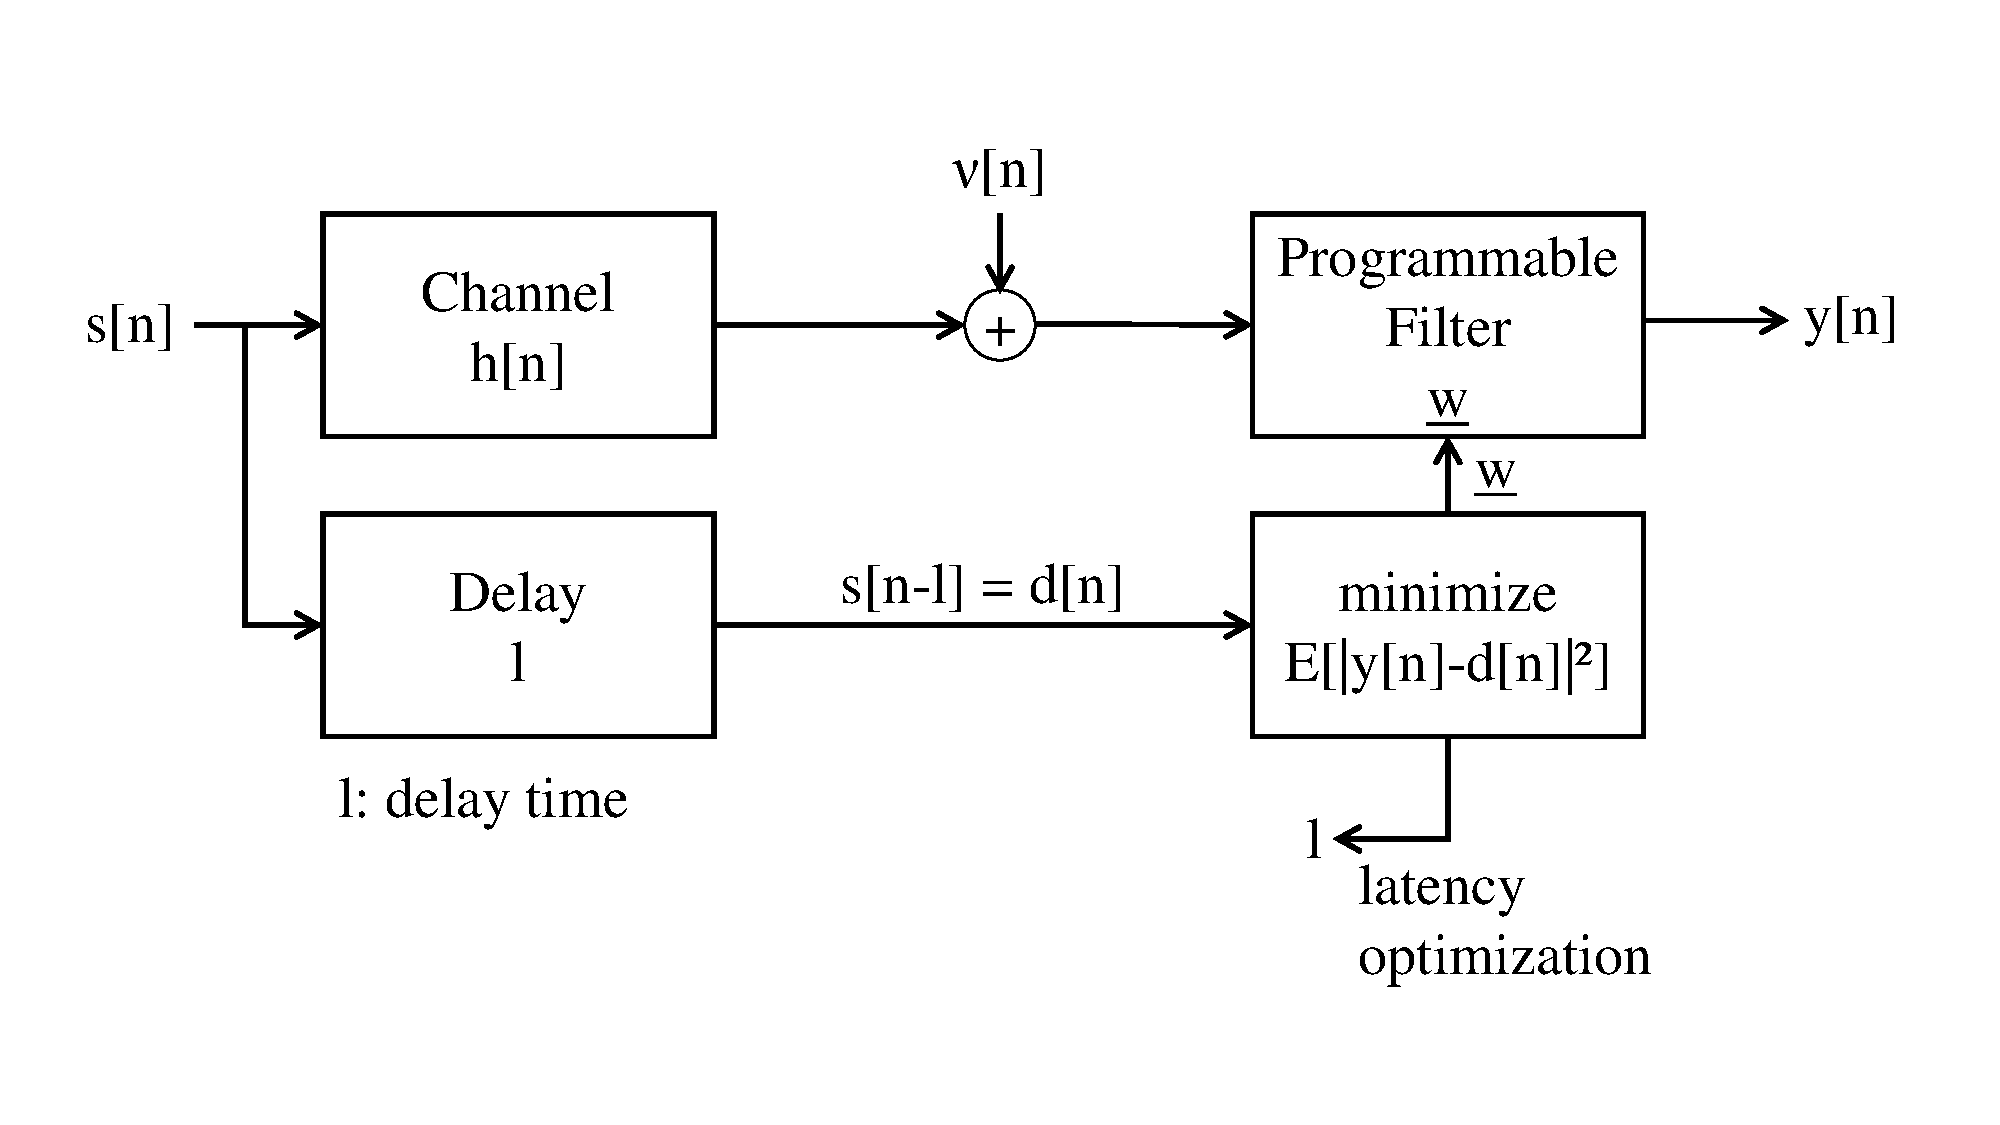
\includegraphics[width=0.80\textwidth, trim =1cm 2cm 1cm 2cm,clip ]{graphics/Optimum_filter_block_diagram.pdf}
	\caption{Basic block diagram of an Optimum Linear Filter}
	\label{fig:Optimum_filter_block_diagram}
\end{figure}

$x[n]=\sum\limits_{k=0}^{K} h[k] \cdot s[n-k]; \qquad K$: Channel memory ($0\leq K$)\\
$y[n]=\sum\limits_{k=0}^{M-1} w_k^* \cdot u[n-k]; \qquad M$: Number of filter coefficients (filter order) ($1\leq M$)\\

$\vec{x}[n] = \mat{x[n]\\ x[n-1]\\ \svdots \\ x[n-M+1]}; \qquad \vec{s}[n]= \mat{s[n]\\ s[n-1]\\ \svdots \\ s[n-N+1]}$\\

$\vec{x}[n] = \underbrace{\mat{h[0] & h[1] & h[2] & \shdots & h[K] & & 0 & \shdots & 0\\
													0 & h[0] & h[1] & h[2] & \shdots & h[K-1] & h[K] & 0 & \shdots & 0\\
													\ddots & \ddots & \ddots & \ddots & \ddots & \ddots & \ddots & \ddots & &\\
													0 & \shdots & 0 & h[0] & h[1] & h[2] & &\shdots & h[K-1] & h[K]}}_{\ma{H}} \cdot \vec{s}[n]$\\
\mybox{$\ma{H}\in \mathbb{C}^{M\times N}$\\$N=M+K \geq M $\\$\quad \Rightarrow$ wide Matrix} \\

$\vec{w} = \mat{w_0\\ w_1\\ \svdots \\w_{M-1}}; \qquad \vec{u}[n]=\vec{x}[n] + \vec{\nu}[n]; \qquad \vec{\nu}[n]$: Noise\\
$y[n] = \vec{w}^H \vec{u}[n] = \vec{w}^H(\vec{x}[n] + \vec{\nu}[n])$\\
\mybox{
$y[n] = \vec{w}^H (\ma{H}\vec{s}[n] + \vec{\nu}[n])$\\
with:\\
$y[n]$: Filter output\\
$\vec{w}^H$: Filter vector\\
$\ma{H}$: Channel matrix\\
$\vec{s}[n]$: Tx-signal vector\\
$\vec{\nu}[n]$: Noise vector
}
\subsection{Correlation between filter output and error in the optimum}
\begin{itemize}
	\item Error signal: $e[n]=d[n] - y[n]$
	\item Cost function: $J=E[|e[n]|^2]$
	\item Optimization: $\vec{w}_{opt} = \text{arg } \min\limits_{\vec{w}} J$
\end{itemize}

\begin{doublespace}

$J=E[e^*[n]\cdot e[n]] = E[(d^*[n] - y^*[n])(d[n]-\underbrace{y[n]}_{\vec{w}^H\vec{u}[n]})]$\\
$\frac{\partial J}{\partial \vec{w}^*} = E[e^*[n](-\vec{u}[n])] \stackrel{!}{=} 0$ (in the optimum)\\
$E[e^*[n]y[n]] = E[e^*[n]\vec{w}^H\vec{u}[n]] \underbrace{=}_{\vec{w}^H\ \text{deterministic}} \vec{w}^H\ E[e^*[n]\vec{u}[n]]=0$\\
in the optimum $\Leftrightarrow E[y[n]e^*[n]] = 0$ (Filter output is uncorrelated with error)\\
If you want to know, whether  a different filter is optimal or not, test if the error and the output are uncorrelated.

\subsection{Determine Optimal Filter Weight \texorpdfstring{$w_{opt}$}{w-opt}}
$J=E[(d^*[n] - y^*[n])(d[n]-y[n])] = \sigma_d^2 - \vec{w}^H\vec{p} - \vec{p}^H \vec{w} + \vec{w}^H \ma{R}\vec{w}$\\
$\sigma_d^2 = E[|d[n]|^2]$\\
$\vec{p} = E[\vec{u}[n]d^*[n]]; \qquad$ correlation vector\\
$\ma{R} = E[\vec{u}[n]\vec{u}^H[n]]; \qquad$ correlation matrix\\
Note: $\ma{R}\geq 0 \qquad$ usually $\ma{R}>0 \Rightarrow \ma{R}^{-1}$ exists\\$\qquad \ma{R}=\ma{R}^H$\\
$\frac{\partial J}{\partial \vec{w}^*}=-\vec{p} + \ma{R}\vec{w} \stackrel{!}{=} 0$\\
\mybox{
$\vec{w}_{opt}=\ma{R}^{-1}\vec{p}$}
$\vec{w}^H_{opt} = \vec{p}^H(\ma{R}^{-1})^H = \vec{p}^H(\ma{R}^{H})^{-1} = \vec{p}^H\ma{R}^{-1}$\\
$J\left.\right|_{\vec{w}=\vec{w}_{opt}}= \sigma_d^2 - \underbrace{\vec{p}^H\ma{R}^{-1}\vec{p}}_{=\vec{w}_{opt}\vec{p}} - \underbrace{\vec{p}^H\ma{R}^{-1}\vec{p} + \underbrace{\vec{p}^H\ma{R}^{-1}\ma{R}\ma{R}^{-1}\vec{p}}_{=\vec{p}^H\ma{R}^{-1}\vec{p}}}_{=0} = \sigma_d^2(1-\underbrace{\frac{\vec{p}^H\ma{R}^{-1}\vec{p}}{\sigma_d^2}}_{|\rho|^2}) \qquad 0\leq|\rho|^2\leq 1$
\end{doublespace}

\begin{figure}[htbp]
	\centering
		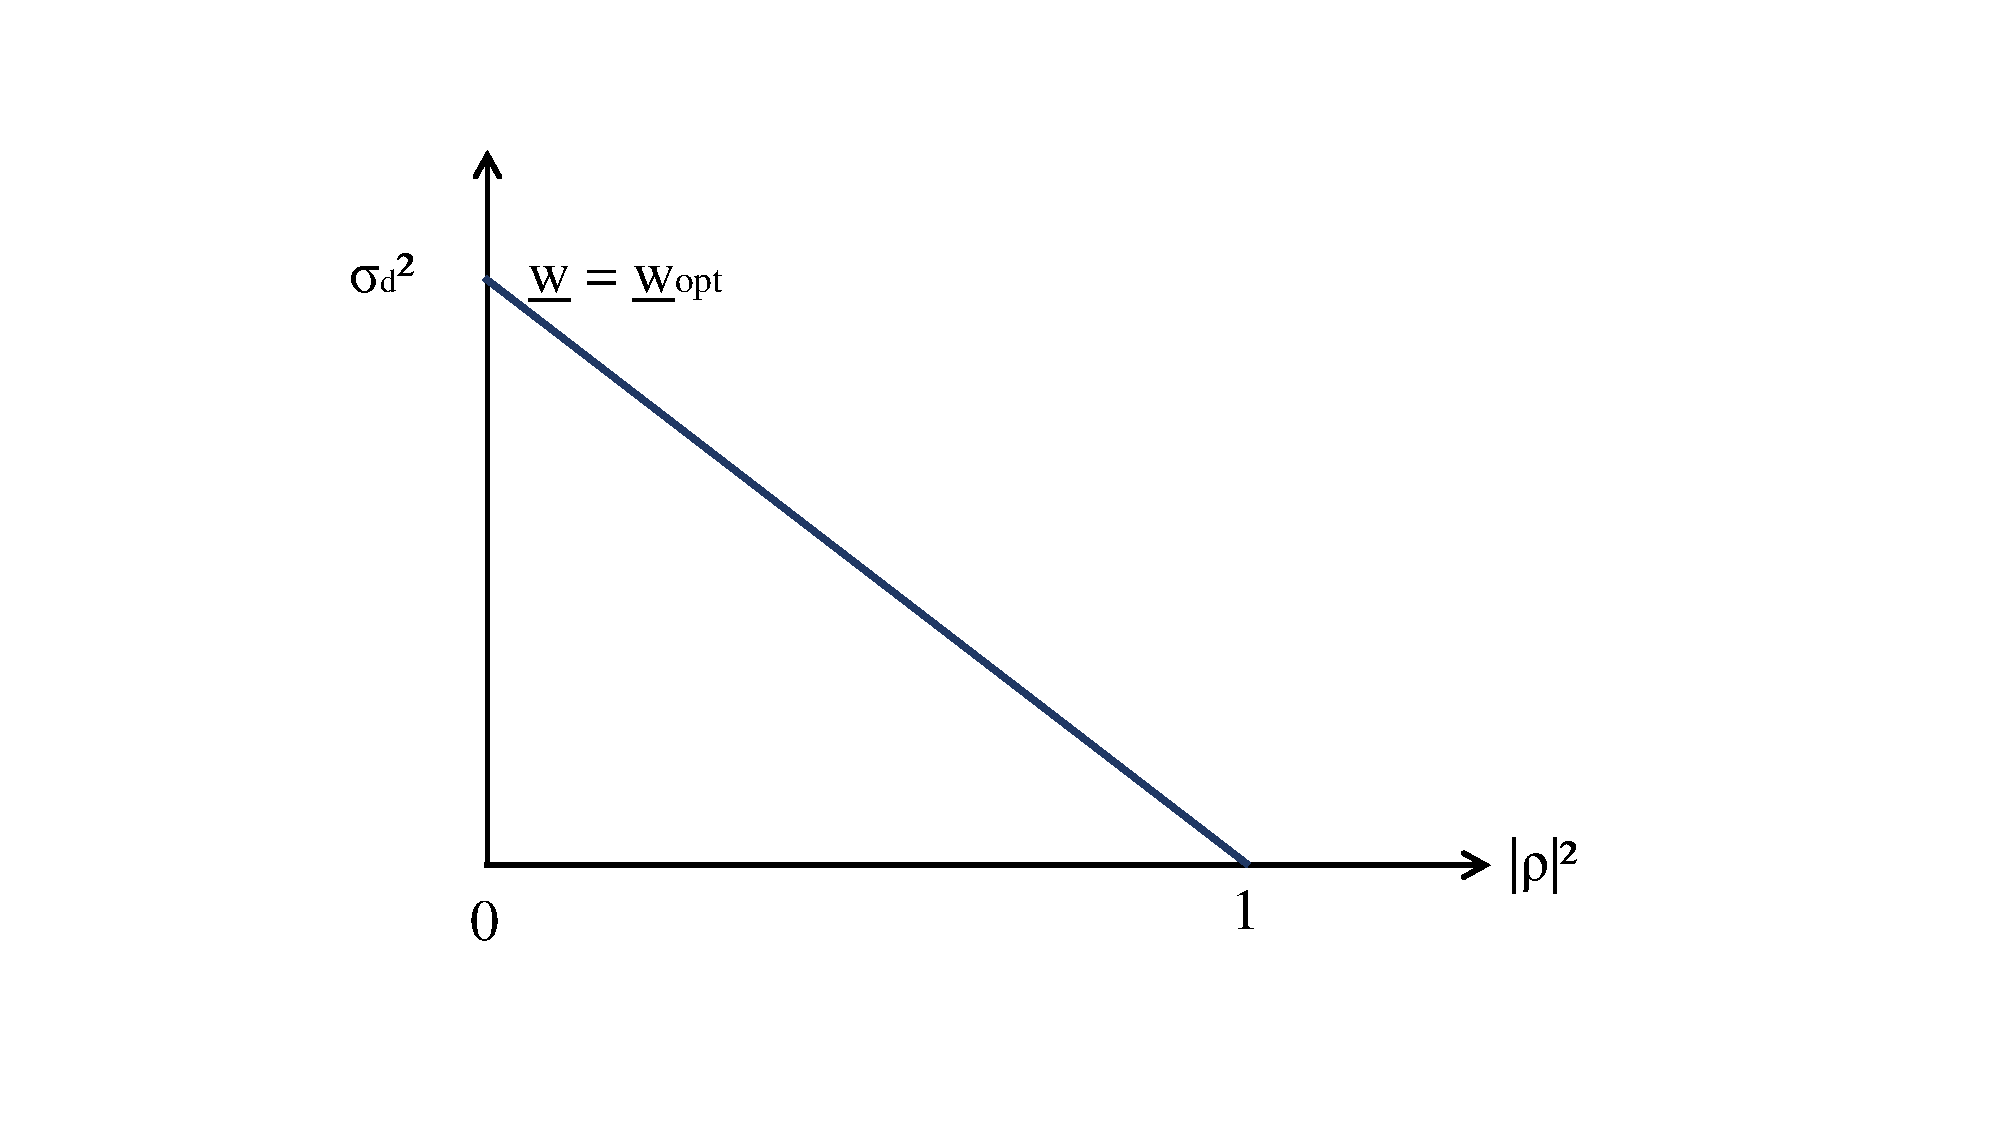
\includegraphics[trim =1cm 2cm 4cm 2cm, clip, width=0.80\textwidth]{graphics/diagram_rho_vs_sigma.pdf}
	\caption{Correlation betweem $\sigma_d^2$ and $|\rho|^2$}
	\label{fig:diagram_rho_vs_sigma}
\end{figure}

\begin{doublespace}
\begin{tabular}{ll}
$J$&$=\sigma_d^2 - \vec{w}^H\vec{p} - \vec{p}^H \vec{w} + \vec{w}^H \ma{R}\vec{w}$\\
&$=\sigma_d^2 - \vec{w}^H\ma{R}\underbrace{\ma{R}^{-1}\vec{p}}_{\vec{w}_{opt}} - \underbrace{\vec{p}^H \ma{R}^{-1}}
_{\vec{w}^H_{opt}} \ma{R} \vec{w} + \vec{w}^H \ma{R}\vec{w} + \vec{p}^H \underbrace{\ma{R}^{-1}\ma{R}\ma{R}^{-1}}_{\ma{R}^{-1}}\vec{p} - \vec{p}^H\ma{R}^{-1}\vec{p}$\\
&$=\sigma_d^2 - \vec{w}^H\ma{R}\vec{w}_{opt} - \vec{w}^H_{opt}\ma{R}\vec{w} + \vec{w}^H\ma{R}\vec{w} + \vec{w}^H_{opt}\ma{R}\vec{w}_{opt} - \vec{p}^H\ma{R}^{-1}\vec{p}$\\
&$=\underbrace{\sigma_d^2 - \vec{p}^H\ma{R}^{-1}\vec{p}}_{J_{min}} + \underbrace{(\vec{w}^H-\vec{w}^H_{opt})}_{\Delta\vec{w}^H}\ma{R} \underbrace{(\vec{w} - \vec{w}_{opt})}_{\Delta\vec{w}}$\\
&$=J_{\text{min}} + \underbrace{\Delta\vec{w}^H\ma{R}\Delta\vec{w}}_{>0 \quad \forall \Delta\vec{w}\neq 0 \quad \text{because } \ma{R}>0}; \qquad \vec{w}=\vec{w}_{opt} + \Delta\vec{w}$
\end{tabular}\\
\textbf{EVD:}\\
$\ma{R} = \ma{Q} \ma{\Lambda} \ma{Q}^H; \qquad \ma{\Lambda} = \mat{\lambda_1 & & \\ & \ddots &\\ & & \lambda_M} > \vec{0}$\\
$J=J_{\text{min}} + \underbrace{\Delta\vec{w}^H \ma{Q}}_{\vec{v}^H} \ma{\Lambda} \underbrace{\ma{Q}^H \Delta\vec{w}}_{\vec{v}} = J_{\text{min}} + \vec{v}^H \ma{\Lambda} \vec{v} = J_{\text{min}} + \sum\limits_{m=1}^{M} \lambda_m |v_m|^2$\\
\end{doublespace}

\begin{doublespace}
$\vec{u}[n] = \ma{H}\vec{s}[n] + \vec{\nu}[n]$\\
\begin{tabular}{ll}
$\ma{R}_u$&$:= E[\vec{u}[n]\vec{u}^H[n]] = E[(\ma{H}\vec{s}[n] + \vec{\nu}[n])(\vec{s}^H[n]\ma{H}^H + \vec{\nu}^H[n])]$\\
&$=\ma{H} \underbrace{E[\vec{s}[n]\vec{s}^H[n]]}_{\ma{R}_s}\ma{H}^H + \ma{H} \underbrace{E[\vec{s}[n]\vec{\nu}^H[n]]}_{\ma{R}_{s\nu}} + \underbrace{E[\vec{\nu}[n]\vec{s}^H[n]]}_{\ma{R}_{\nu s}= \ma{R}_{s\nu}^H}\ma{H}^H + \underbrace{E[\vec{\nu}[n]\vec{\nu}^H[n]]}_{\ma{R}_\nu}$\\
\end{tabular}\\
In the following: $\ma{R}_{\nu s} = 0$\\
\mybox{
$\ma{R}_u = \ma{H} \ma{R}_s \ma{H}^H + \ma{R}_\nu := \ma{R}$
}

\begin{flalign*}
\vec{p} &= E[\vec{u}[n]d^*[n]]=E[(\ma{H}\vec{s}[n] + \vec{\nu}[n])d^{*}[n]]; \qquad d[n]=s[n-l]&&\\
&=\ma{H}\,E[\vec{s}[n]d^*[n]] + \underbrace{E[\vec{\nu}[n]\cdot s^{*}[n-l]]}_{=\vec{0}}&&\\
&=\ma{H}\,E[\vec{s}[n]\underbrace{s^*[n-l]}_{\vec{s}^H[n]\cdot \vec{e}_{l+1}}]&&
\end{flalign*}

$\vec{s}^H=\mat{s^*[n] & s^*[n-1] & s^*[n-2] & \shdots & s^*[n-l] & s^*[n-l-1] & \shdots & s^*[n-N+1]}$\\
$\vec{e}^T_{l+1} = \mat{0 & 0 & 0 & \shdots & \underbrace{1}_{l+1} & 0 & \shdots & 0]}$\\
$\vec{p}= \ma{H} E[\vec{s}[n]\vec{s}^H[n]] \vec{e}_{l+1}$\\
\mybox{
$\vec{p}= \ma{H} \ma{R}_s \vec{e}_{l+1}$\\
$\vec{w}_{opt} = \ma{R}^{-1}_u \vec{p} = (\ma{H}\ma{R}_s\ma{H}^H+\ma{R}_\nu)^{-1} \ma{H}\ma{R}_s\vec{e}_{l+1}$\\
$\ma{H}\in \mathbb{C}^{M\times N}$
}\\
\end{doublespace}

\begin{doublespace}
\subsubsection{Filter Weight \texorpdfstring{$w_{opt}$}{w-opt} for tall Channel matrices}
\textbf{Example: Receiver with two antennas}
\begin{figure}[htbp]
	\centering
		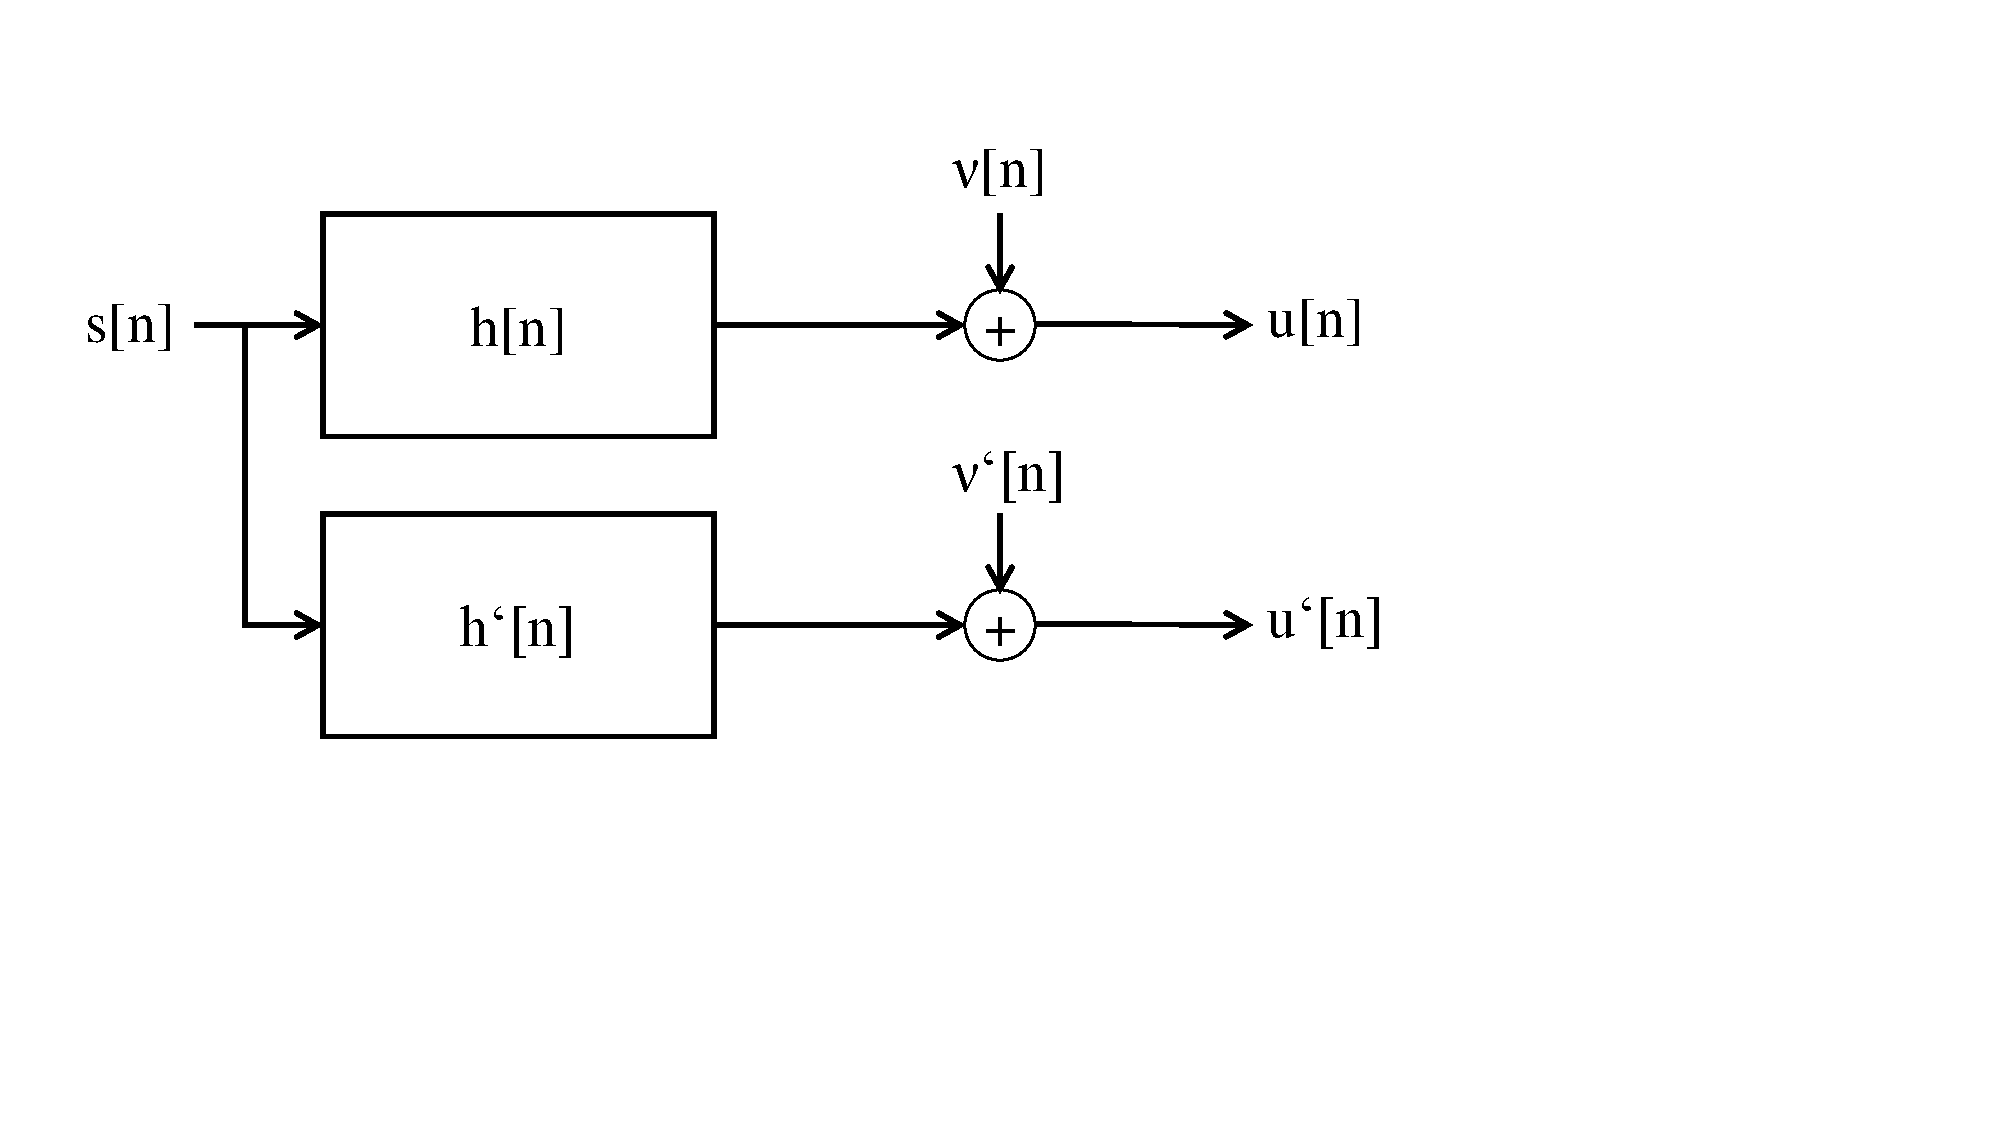
\includegraphics[trim =1cm 5cm 5cm 2cm, clip, width=0.70\textwidth]{graphics/Block_diagram_2_antenna_RX.pdf}
	\caption{Block diagram of a receiver with two inputs (antennas)}
	\label{fig:Block_diagram_2_antenna_RX}
\end{figure}

$\vec{u}[n] = \ma{H} \vec{s}[n] + \vec{\nu}[n]$\\
$\vec{u}'[n] = \ma{H}' \vec{s}[n] + \vec{\nu}'[n]$\\
$\underbrace{\mat{\vec{u}[n]\\ \vec{u}'[n]}}_{\vec{\tilde{u}}[n]} = \underbrace{\mat{\ma{H}\\ \ma{H}'}}_{\ma{\tilde{H}}} \vec{s}[n] + \underbrace{\mat{\vec{\nu}[n]\\ \vec{\nu}'[n]}}_{\ma{\tilde{\nu}}[n]}$\\
$\vec{\tilde{u}}[n] = \ma{\tilde{H}} \vec{s}[n] + \vec{\tilde{\nu}}[n]; \qquad \ma{\tilde{H}}\in \mathbb{C}^{2M\times N}$\\
$\ma{\tilde{H}}$ could have more rows than columns:\\
$(\ma{\tilde{H}}\ma{\tilde{R}}_s\ma{\tilde{H}}^H)\in\mathbb{C}^{2M\times 2M}$\\
$\Rightarrow$ If $2M > N$ we have a problem with the rank.
\\ \ \\

\mybox{
\textbf{Sherman-Morrison-Woodburry Identity}\\
Given $\ma{A}\in\mathbb{C}^{M\times M},\, \text{rank} \ma{A}=M$ and $\ma{C}\in\mathbb{C}^{N\times N},\, \text{rank} \ma{C}=N$ and $\ma{B}\in\mathbb{C}^{M\times N}$ and $\ma{D}\in\mathbb{C}^{N\times M}$, then:\\
$(\ma{A}+\ma{B}\ma{C}\ma{D})^{-1} = \ma{A}^{-1} - \ma{A}^{-1}\ma{B}(\ma{C}^{-1}+\ma{D}\ma{A}^{-1}\ma{B})^{-1}\ma{D}\ma{A}^{-1}$
}\\

\textbf{Proof:}\\
$(\ma{A}^{-1} - \ma{A}^{-1}\ma{B}(\ma{C}^{-1}+\ma{D}\ma{A}^{-1}\ma{B})^{-1}\ma{D}\ma{A}^{-1})(\ma{A}+\ma{B}\ma{C}\ma{D})$\\
$=\underbrace{\ma{A}^{-1}\ma{A}}_{\ma{I}} + \ma{A}^{-1}\ma{B}\ma{C}\ma{D} - \ma{A}^{-1}\ma{B}(\ma{C}^{-1}+\ma{D}\ma{A}^{-1}\ma{B})^{-1}\ma{C}^{-1}\ma{C}\ma{D}\underbrace{\ma{A}^{-1}\ma{A}}_{\ma{I}}-\ma{A}^{-1}\ma{B}(\ma{C}^{-1}+\ma{D}\ma{A}^{-1}\ma{B})^{-1}\ma{D}\ma{A}^{-1}\ma{B}\ma{C}\ma{D}$\\
$=\ma{I} + \ma{A}^{-1}\ma{B}(\ma{I}\underbrace{-(\ma{C}^{-1}+\ma{D}\ma{A}^{-1}\ma{B})^{-1}\ma{C}^{-1}-(\ma{C}^{-1}+\ma{D}\ma{A}^{-1}\ma{B})^{-1}\ma{D}\ma{A}^{-1}\ma{B}}_{-\underbrace{(\ma{C}^{-1}+\ma{D}\ma{A}^{-1}\ma{B})^{-1}(\ma{C}^{-1}+\ma{D}\ma{A}^{-1}\ma{B})}_{\ma{I}}})\ma{C}\ma{D}$\\
$=\ma{I}$\qed\\ \ \\

Applying the Sherman-Morrison-Woodburry Identity on $\vec{w}_{opt}$ with $\ma{B}=\ma{H}$, $\ma{C}=\ma{R}_s$, $\ma{D}=\ma{H}^H$ and $\ma{A}=\ma{R}_{\nu}$ we get:\\
\begin{flalign*}
\vec{w}_{opt}&=(\ma{H}\ma{R}_s\ma{H}^H+\ma{R}_{\nu})^{-1}\ma{H}\ma{R}_s\vec{e}_{l+1}&&\\
&=(\ma{R}_{\nu}^{-1} - \ma{R}_{\nu}^{-1}\ma{H}(\ma{R}_s^{-1}+\ma{H}^H\ma{R}_{\nu}^{-1}\ma{H})^{-1}\ma{H}^H\ma{R}_{\nu}^{-1})\ma{H}\ma{R}_s\vec{e}_{l+1}&&\\
&=\ma{R}_{\nu}^{-1}\ma{H}(\underbrace{\ma{I}}_{(\ma{R}_{s}^{-1}+\ma{H}^H\ma{R}_{\nu}^{-1}\ma{H})^{-1}(\ma{R}_{s}^{-1}+\ma{H}^H\ma{R}_{\nu}^{-1}\ma{H})}(-(\ma{R}_{s}^{-1}+\ma{H}^H\ma{R}_{\nu}^{-1}\ma{H})^{-1}\ma{H}^H\ma{R}_{\nu}^{-1}\ma{H})\ma{R}_{s}\vec{e}_{l+1}&&\\
&=\ma{R}_{\nu}^{-1}\ma{H}(\ma{R}_{s}^{-1}+\ma{H}^H\ma{R}_{\nu}^{-1}\ma{H})^{-1}\underbrace{(\ma{R}_s^{-1}+\underbrace{\ma{H}^H\ma{R}_{\nu}^{-1}\ma{H}-\ma{H}^H\ma{R}_{\nu}^{-1}\ma{H}}_{=0})\ma{R_s}}_{=\ma{I}}\vec{e}_{l+1}
\end{flalign*}
\mybox{
\begin{flalign}
\vec{w}_{opt}&=\ma{R}_{\nu}^{-1}\ma{H}\underbrace{(\ma{R}_s^{-1}+\ma{H}^H\ma{R}_{\nu}^{-1}\ma{H})^{-1}}_{N\times N}\vec{e}_{l+1}&&\label{eq:wopt_1}\\
&=\underbrace{(\ma{R}_{\nu}+\ma{H}\ma{R}_{s}\ma{H}^H)^{-1}}_{M\times M}\ma{H}\ma{R}_s\vec{e}_{l+1}\label{eq:wopt_2}
\end{flalign}
}
$\ma{H}\in\mathbb{C}^{M\times N}$\\
If $M<N$ use equation \eqref{eq:wopt_2}: $M$ equations in $M$ unknowns\\
If $N<M$ use equation \eqref{eq:wopt_1}: $N$ equations in $N$ unknowns\\
\textbf{Note: processor \& memory load}\\
$\ma{A}\vec{x}=\vec{b}:\quad \ma{A}\in\mathbb{C}^{n\times n}$\\
\begin{tabular}{ll}
Solve for \vec{x}: &computational load $\sim n^3$\\
&memory $\sim n^2$\\
\end{tabular}
\end{doublespace}

\begin{doublespace}
\textbf{Note: Inter-Symbol-Interference}\\
$y[n]=\vec{w}^H\vec{u}[n] = \vec{w}(\ma{H}\vec{s}[n]+\vec{\nu}[n]) = \vec{w}^H(\underbrace{\mat{\vec{h}_1&\vec{h}_2&\shdots&\vec{h}_N}}_{\ma{H}}\underbrace{\vec{s}[n]}_{\mat{s[n]\\s[n-1]\\\svdots\\s[n-M+1]}}+\vec{\nu}[n])$\\
$d[n]=s[n-l]$\\
$y[n]=\vec{w}^H(\vec{h}_{l+1}\underbrace{\vec{s}[n-l]}_{\text{signal of interest}}+\underbrace{\sum\limits_{k=1; k\neq l+1}^{N}\vec{h}_k \vec{s}[n-k]}_{\text{Inter-Symbol-Interference}}+\underbrace{\vec{\nu}[n])}_{\text{Noise}}$\\
\subsection{Filter with different kinds of Noise}

\subsubsection{Special case: White Noise \& White Signal} 
$\ma{R}_s=\sigma_d^2\ma{I};\qquad \ma{R}_\nu=\sigma_\nu^2\ma{I}$\\
$\vec{w}_{opt}=(\frac{\sigma_u^2}{\sigma_d^2}\ma{I}+\ma{H}\ma{H}^H)^{-1}\ma{H}\vec{e}_{l+1}$\\
\\
\subsubsection{Case 1: High SNR (signal to noise ratio)}
$\ma{H}\in\mathbb{C}^{M\times N}; \qquad M<N$\\
$\text{rank}\ma{H}=M$ (full rank \ma{H})\\
$\ma{H}=\ma{U}_1\ma{\Sigma}_1\ma{V}_1^H \underbrace{=}_{\text{rank}\ma{H}=M} \ma{U}\ma{\Sigma}_1\ma{V}_1^H$
\begin{flalign*}
(\ma{H}\ma{H}^H)^{-1}\ma{H} &= (\ma{U}\ma{\Sigma}_1\ma{V}_1^H\ma{V}_1\ma{\Sigma}_1\ma{U}^H)^{-1}\ma{U}\ma{\Sigma}_1\ma{V}_1^H&&\\
&=(\ma{U}\ma{\Sigma}_1^2\ma{U}^H)^{-1}\ma{U}\ma{\Sigma}_1\ma{V}_1^H&&\\
&=\ma{U}\ma{\Sigma}_1^{-2}\underbrace{\ma{U}^H\ma{U}}_{\ma{I}}\ma{\Sigma}_1\ma{V}_1^H&&\\
&=\ma{U}\ma{\Sigma}_1^{-1}\ma{V}_1^H=\ma{U}_1\ma{\Sigma}_1^{-1}\ma{V}_1^H=(\ma{V}_1\ma{\Sigma}_1^{-1}\ma{U}^H)^H&&\\
&=(\ma{H}^+)^H = (\ma{H}^H)^+
\end{flalign*}
$\lim\limits_{\frac{\sigma_d^2}{\sigma_\nu^2}\rightarrow\infty}\vec{w}_{opt}=(\ma{H}\ma{H}^H)^{-1}\ma{H}\vec{e}_{l+1}=\underbrace{(\ma{H}^H)^+}_{\text{Moore-Penrose-Pseudo-Inverse}}\vec{e}_{l+1}$\\ \\
No optimal solution because:\\
Try: $\vec{w}^H\ma{H}\stackrel{!}{=}\vec{e}_{l+1}^T;\quad y[n]=\underbrace{\vec{w}^H\ma{H}}_{\vec{e}_{l+1}^T}\vec{s}[n]=\vec{s}[n-1]$\\
However it does not work!\\
$\ma{H}^H\vec{w}=\vec{e}_{l+1}$\\
$\ma{H}^H\in\mathbb{C}^{N\times M}\qquad \text{with } M<N$\\
Number of degrees of freedom = $M$\\
Number of constraints = $N>M$\\
$\Rightarrow$ No exact solution exists!\\
$\Rightarrow$ LS-Solution (least square)\\
\mybox{
$\vec{w}_{LS}=(\ma{H}^H)^+\vec{e}_{l+1}$}
\mybox{
For high SNR the optimum filter tries to suppress the interference but lack DoF (Degrees of Freedom) to do it perfectly.\\
$\vec{w}_{LS}=\arg\min\limits_{\vec{w}}||\vec{w}^H\ma{H}-\vec{e}_{l+1}||_2^2$\\
}\\
The higher the dimensions, the better the outcome of the filter. \\ \ \\
\textbf{Work-around: Block processing}\\
at Tx: pre-pend K guard symbols\\
at Rx: discard first K received symbols\\
\textbf{Example:}\\
$K=2$ (number of \textcolor[rgb]{1,0,0}{guard symbols}), $\quad M=4$ (number of payload symbols)\\
$\mat{u[n]\\u[n-1]\\u[n-2]\\u[n-3]}=\vec{\nu}[n] + \mat{h_0&h_1&h_2&0&0&0\\ 0&h_0&h_1&h_2&0&0\\ 0&0&h_0&h_1&h_2&0\\ 0&0&0&h_0&h_1&h_2}\mat{s[n]\\s[n-1]\\s[n-2]\\s[n-3]\\\textcolor[rgb]{1,0,0}{s[n]}\\\textcolor[rgb]{1,0,0}{s[n-1]}}$\\
$\ma{\overset{\circ}{H}}=\mat{h_0&h_1&h_2&0\\ 0&h_0&h_1&h_2\\ h_2&0&h_0&h_1\\ h_1&h_2&0&h_0}$ (cyclic matrix)\\
$\ma{\overset{\circ}{H}}$ is invertible \pfeil with no noise, we get a perfect solution with losing bandwidth efficiency\\
$\vec{s}[n] = \mat{s[n]\\s[n-1]\\s[n-2]\\s[n-3]}$\\
Example MATLAB-code: \lstinline !Q=fft(eye(M))/sqrt(M)!\\
$\ma{Q}^H\mat{H}\mat{Q}=\mat{a_1& & & \\ &a_2& & \\ & &a_3& \\ & & &a_4}$\\
$\mat{a_1&a_2&a_3&a_4}=\text{fft}(\mat{h_0&h_1&h_2&0}) \Rightarrow$ OFDM (Orthogonal Frequency Division Multiplexing)\\ \ \\

\subsubsection{Case 2: Low SNR (High Noise)}
$\frac{\sigma_\nu^2}{\sigma_d^2}\rightarrow\infty$\\
$y[n]\approx\vec{w}^H(\vec{h}_{l+1}s[n-l]+\vec{\nu}[n])$\\
$SNR=\frac{E[|y[n]|^2|\vec{\nu}[n]=\vec{0}]}{E[|y[n]|^2|s[n-l]=0]} = \frac{\sigma_d^2|\vec{w}^H\vec{h}_{l+1}|^2}{\sigma_\nu^2\vec{w}^H\vec{w}}$\\

\textbf{Calculation of the SNR with respect to variances of signal and noise}\\
System: $y[n]=\vec{w}^H\vec{u}[n]=\vec{w}^H\ma{H}\vec{s}[n]+\vec{w}^H\vec{\nu}[n]$\\
\with $\vec{s}[n]=\vec{e}_{l+1}\cdot d[n]$

\parbox{0.5\textwidth}{
\begin{align*}
&E[|y[n]|^2|\vec{\nu}[n]=\vec{0}]\\
=& E[(\vec{w}^H\ma{H}\vec{s}[n])^*(\vec{w}^H\ma{H}\vec{s}[n])]\\
=& E[(\vec{s}[n]^H\ma{H}^H\vec{w})(\vec{w}^H\ma{H}\vec{s}[n])]\\
=& E[\vec{s}[n]^H\ma{H}^H\vec{w}\vec{w}^H\ma{H}\vec{s}[n]]\\
=&E[d[n]^*d[n]\cdot\vec{e}_{l+1}^H\ma{H}^H\vec{w}\vec{w}^H\ma{H}\vec{e}_{l+1}]\\
=&E[\abs{d[n]}^2\cdot\underbrace{\vec{h}_{l+1}^H\vec{w}}_{\in\mathbb{C}^{1\times 1}}\underbrace{\vec{w}^H\vec{h}_{l+1}}_{\in\mathbb{C}^{1\times 1}}]\\
=& E[\underbrace{\abs{d[n]}^2}_{\text{random}}\cdot\underbrace{\abs{\vec{w}^H\vec{h}_{l+1}}^2}_{\text{deterministic}}]\\
=& E[\abs{d[n]}^2]\cdot\abs{\vec{w}^H\vec{h}_{l+1}}^2]\\
=& \sigma_d^2\cdot\abs{\vec{w}^H\vec{h}_{l+1}}^2\\
\end{align*}
}
\parbox{0.5\textwidth}{
\begin{align*}
&E[|y[n]|^2|s[n-l]=0]\\
=&E[(\vec{w}^H\vec{\nu}[n])^*(\vec{w}^H\vec{\nu}[n])]\\
=&E[(\vec{w}^H\vec{\nu}[n])^H(\vec{w}^H\vec{\nu}[n])]\\
=&E[\vec{\nu}[n]^H\vec{w}\vec{w}^H\vec{\nu}[n]]\\
=&E[\tr(\vec{\nu}[n]^H\vec{w}\vec{w}^H\vec{\nu}[n])]\\
=&E[\tr(\vec{w}^H\vec{\nu}[n]\vec{\nu}[n]^H\vec{w})]\\
=&\tr(\vec{w}^H E[\vec{\nu}[n]\vec{\nu}[n]^H]\vec{w})\\
=&\tr(\vec{w}^H(\sigma_\nu^2 \ma{I})\vec{w})\\
=&\sigma_\nu^2\cdot\tr(\underbrace{\vec{w}^H\vec{w}}_{\in\mathbb{C}^{1\times 1}})=\sigma_\nu^2\cdot\vec{w}^H\vec{w}\\
\end{align*}}

\textbf{Mathematical derivation of Cauchy-Schwarz-Inequality:}\\
$\vec{z}:=\vec{h}-\vec{w}\frac{\vec{w}^H\vec{h}}{\vec{w}^H\vec{w}}$
\begin{flalign*}
\vec{z}^H\vec{z}&=(\vec{h}^H-\frac{\vec{h}^H\vec{w}}{\vec{w}^H\vec{w}}\vec{w})(\vec{h}-\vec{w}\frac{\vec{w}^H\vec{h}}{\vec{w}^H\vec{w}})&&\\
&=\vec{h}^H\vec{h}-\frac{(\vec{h}^H\vec{w})(\vec{w}^H\vec{h})}{\vec{w}^H\vec{w}}-\frac{(\vec{h}^H\vec{w})(\vec{w}^H\vec{h})}{\vec{w}^H\vec{w}}+\frac{(\vec{h}^H\vec{w})(\vec{w}^H\vec{h})\vec{w}^H\vec{w}}{(\vec{w}^H\vec{w})(\vec{w}^H\vec{w})}&&\\
&=\vec{h}^H\vec{h}-\frac{|\vec{w}^H\vec{h}|^2}{\vec{w}^H\vec{w}}\geq 0
\end{flalign*}
\mybox{
Cauchy-Schwarz-Inequality:\\
$\frac{|\vec{w}^H\vec{h}|^2}{\vec{w}^H\vec{w}}\leq\vec{h}^H\vec{h}$
}
$SNR=\frac{\sigma_d^2}{\sigma_\nu^2}\frac{|\vec{w}^H\vec{h}_{l+1}|^2}{\vec{w}^H\vec{w}}\leq\frac{\sigma_d^2}{\sigma_\nu^2}\vec{h}_{l+1}^H\vec{h}_{l+1}$\\
$\vec{w}_{MF}=\arg\max\limits_{\vec{w}}SNR=\const \cdot \vec{h}_{l+1}\with \const\neq 0\qquad$ where MF stands for "matched filter"\\
try: $SNR\left.\right|_{\vec{w}=\vec{w}_{MF}}=\frac{\sigma_d^2}{\sigma_\nu^2}\frac{\left|\vec{h}_{l+1}^H\vec{h}_{l+1}\right|^2\cdot|\const|^2}{\vec{h}_{l+1}^H\vec{h}_{l+1}\cdot|\const|^2}=\frac{\sigma_d^2}{\sigma_\nu^2}\vec{h}_{l+1}^H\vec{h}_{l+1}$\\
$\vec{w}=\vec{w}_{MF}$ achieves an upper bound of the SNR.\\
\mybox{
Optimum Filter Solution:\\
$\vec{w}_{opt}=\underbrace{\frac{\sigma_d^2}{\sigma_\nu^2}}_{\const}\vec{h}_{l+1}=\vec{w}_{MF}$}
$\lim\limits_{\frac{\sigma_d^2}{\sigma_\nu^2}\rightarrow0}\vec{w}_{opt}=\vec{w}_{MF}\sim\vec{h}_{l+1}$
\end{doublespace}

\subsection{Steepest Descent Algorithm (SDA)}
$\vec{w}_{opt}=\ma{R}^{-1}\vec{p},\qquad \ma{R}\vec{w}_{opt}=\vec{p}$\\
One method to solve this problem woulbd be the Gauß-Elimination but since \ma{R} and \vec{p} usually change it is neccessary to recalulate everything when ever something changes. This would lead to an enormouse effort. So an iterative solution would be more productive.\\
\textbf{Iterative solution:}\\
\begin{doublespace}
$\vec{w}[n+1]=\vec{w}[n]+\Delta\vec{w}[n]$\\
$J=\sigma_d^2-\vec{w}^H\vec{p}-\vec{p}^H\vec{w}+\vec{w}^H\ma{R}\vec{w};\quad \ma{R}>\vec{0}; \qquad \ma{R}=\ma{R}^H$\\
$dJ=\left(\frac{\partial J}{\partial \vec{w}}\right)^T d\vec{w} + \left(\frac{\partial J}{\partial \vec{w^*}}\right)^T d\vec{w}^*$\\
\with $\left(\frac{\partial J}{\partial \vec{w}}\right)^T d\vec{w} = \left(\left(\frac{\partial J^*}{\partial \vec{w^*}}\right)^T d\vec{w}^*\right)^*\underbrace{=}_{J\underbrace{=}_{J\in\mathbb{R}}J^*}\left(\left(\frac{\partial J}{\partial \vec{w^*}}\right)^T d\vec{w}^*\right)^*$ we get:\\
$dJ=2\Re{\left(\frac{\partial J}{\partial \vec{w}^*}\right)^T d\vec{w}^*}$\\
$dJ=2\Re{\left(\frac{\partial J}{\partial \vec{w}^*}\right)^H d\vec{w}} \leq 2 \left|\left(\frac{\partial J}{\partial \vec{w}^*}\right)^H d\vec{w}\right|$\\
$d\vec{w}=\frac{\partial J}{\partial\vec{w}^*}\cdot \const^*;\qquad \const<0$\\
$\Delta\vec{w}[n]=-\mu\frac{\partial J}{\partial\vec{w}^*[n]};\qquad \mu>0$\\
$\frac{\partial J}{\partial \vec{w}^*[n]}=-\vec{p}+\ma{R}\vec{w}[n]$\\
\begin{flalign*}
\vec{w}[n+1]&=\vec{w}[n]+\Delta\vec{w}[n] = \vec{w}[n]-\mu\left(\vec{p}+\ma{R}\vec{w}[n]\right);\qquad \mu>0&&\\
&=(\ma{I}-\mu\ma{R})\vec{w}[n]+\mu\vec{p}
\end{flalign*}

Does $\vec{w}[n],\,\vec{w}[n+1],\ldots$ converge to $\vec{w}_{opt}$?\\
$\vec{c}[n]=\vec{w}[n]-\vec{w}_{opt}$\\
$\underbrace{c[n+1]+\vec{w}_{opt}}_{=\vec{w}[n+1]}=(\ma{I}-\mu\ma{R})\underbrace{\vec{c}[n]+\vec{w}_{opt}}_{\vec{w}[n]}+\mu\vec{p}$\\
$c[n+1]=(\ma{I}-\mu\ma{R})\vec{c}[n]-\underbrace{\mu\ma{R}\overbrace{\vec{w}_{opt}}^{\ma{R}^{-1}\vec{p}}+\mu\vec{p}}_{=\vec{0}}$\\
\mybox{
$c[n+1]=(\ma{I}-\mu\ma{R})\vec{c}[n]$
}\\
Does $c[n],\,c[n+1],\,\ldots$ converge to \vec{0}?\\
EVD: $\ma{R}=\ma{Q}\ma{\Lambda}\ma{Q}^{-1}\underbrace{=}_{\ma{R}=\ma{R}^H}\ma{Q}\ma{\Lambda}\ma{Q}^{H}$\\
$\ma{\Lambda}=\mat{\lambda_1&&&&\\&\lambda_2&&&\\&&\lambda_3&&\\&&&\ddots&\\&&&&\lambda_M};\quad \lambda_i>0;\quad i\in \{1,2,\ldots,M\};\qquad (\ma{R}>0)$\\
\begin{flalign*}
\vec{c}[n+1]&=(\ma{I}-\mu\underbrace{\ma{Q}\ma{\Lambda}\ma{Q}^{H}}_{=\ma{R}})\vec{c}[n]=(\underbrace{\ma{Q}\ma{Q}^H}_{=\ma{I}}-\mu\ma{Q}\ma{\Lambda}\ma{Q}^{H})\vec{c}[n]&&\\
&=\ma{Q}(\ma{I}-\mu\ma{\Lambda})\ma{Q}^H\vec{c}[n]
\end{flalign*}
$\underbrace{\ma{Q}^H\vec{c}[n+1]}_{\vec{z}[n+1]}=(\ma{I}-\mu\ma{\Lambda})\underbrace{\ma{Q}^H\vec{c}[n]}_{\vec{z}[n]}$\\
\mybox{
$\vec{z}[n+1]=(\ma{I}-\mu\ma{\Lambda})\vec{z}[n]$
}\\
$\vec{z}[n]=\mat{z_1[n]&z_2[n]&\shdots&z_M[n]}^T$\\
\mybox{
$z_k[n+1]=(1-\mu\lambda_k)z_k[n];\qquad 1\leq k\leq M$
}\\
$z_k[n],\,z_k[n+1]\ldots$ converge to 0 if and only if $\left|1-\mu\lambda_k\right|<1;\qquad \forall k$\\
\textbf{case 1:} $1-\mu\lambda_k\geq 0\qquad \left[\mu\leq \frac{1}{\lambda_k}\right]$
\begin{flalign*}
\text{then }1-\mu\lambda_k&<1&&\\
-\mu\lambda_k&<0; \qquad \mu>0,\quad \lambda_l>0&&\\
-\mu&<0&&\\
\mu&>0
\end{flalign*}
\mybox{
$0<\mu\leq\frac{1}{\lambda_k}$
}\\ \ \\
\textbf{case 2:} $1-\mu\lambda_k\leq 0\qquad \left[\mu\geq \frac{1}{\lambda_k}\right]$
\begin{flalign*}
\text{then }-1+\mu\lambda_k&<1&&\\
\mu\lambda_k&<2&&\\
\mu&<\frac{2}{\lambda_k}
\end{flalign*}
\mybox{
$\frac{1}{\lambda_k}\leq\mu\leq\frac{2}{\lambda_k}$
}
\mybox{
\textbf{Case 1 \& Case 2:}\\
$\Rightarrow 0<\mu<\frac{2}{\lambda_k} \Leftrightarrow z_k[n],\,z_k[n+1],\,\ldots$ converges to 0.}\\ \ \\
\mybox{
\textbf{Key results:}\\
$\vec{w}[n],\,\vec{w}[n+1],\ldots$ converge to $\vec{w}_{opt}$ iff\\
$0\leq\mu\leq\frac{2}{\lambda_{max}} \qquad \lambda_{max}=\text{ maximum Eigenvalue of }\ma{R}$
}\\ \\
\textbf{Computation of $\lambda_{max}$ is costly!}\\
$\underbrace{\sum\limits_{k=1}^M\lambda_k}_{\text{tr}\ma{R}} > \lambda_{max} < \tr\ma{R}$\\
$0<\mu<\frac{2}{\text{tr}\ma{R}}<\frac{2}{\lambda_{max}}$\\
\end{doublespace}
$\text{tr}\ma{R}$ is cheap to compute. Therfor in practice  $0<\mu<\frac{2}{\text{tr}\ma{R}}$ can be used. This is sufficeint for convergence. But usually one is interested in using an optimum step-size $\mu$ to achive optimum performance of the algorithm.

\subsubsection{Optimum step-size \texorpdfstring{$\mu$}{}}
\begin{figure}[H]
	\centering
		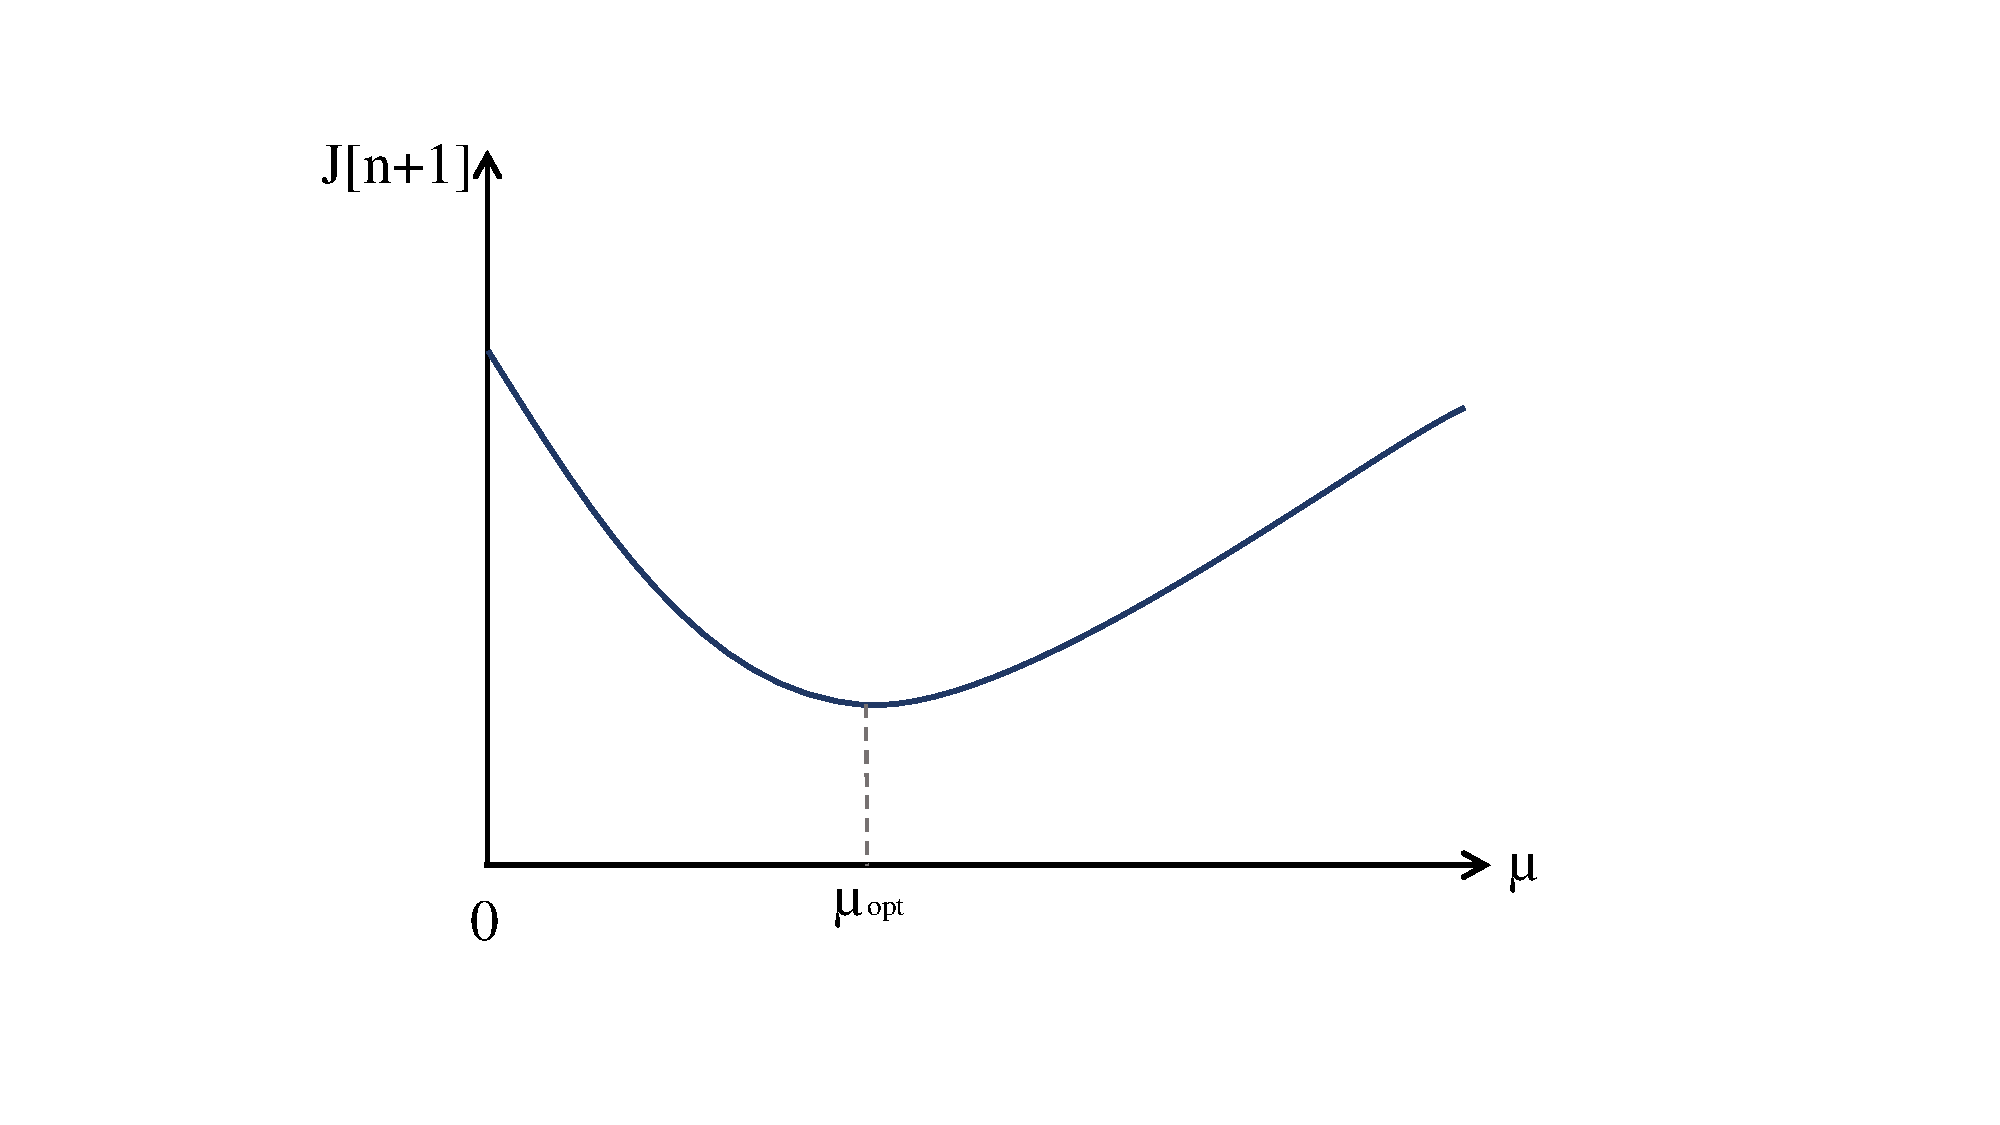
\includegraphics[trim =1cm 3cm 5cm 2cm, clip, width=0.70\textwidth]{graphics/Optimum_step_size_examplepdf.pdf}
	\caption{Example characteristics of the cost function $J[n+1]$ plotted over the step-size $\mu$}
	\label{fig:Optimum_step_size_examplepdf}
\end{figure}
\begin{doublespace}
Solve $\frac{\partial J[n+1]}{\partial \mu^*}=0$ for $\mu=\mu_{opt}$:\\
$J[n+1]=\sigma_d^2-\vec{P}^H\vec{w}[n+1]-\vec{w}^H[n+1]\vec{P}+\vec{w}^H[n+1]\ma{R}\vec{w}[n+1]$\\
$\vec{w}[n+1]=\vec{w}[n]+\mu\vec{r}[n]\quad$ with $\vec{r}[n]=\vec{p}-\ma{R}\vec{w}[n]$\\
\mybox{
$\mu_{opt}=\frac{\vec{r}^H[n]\vec{r}[n]}{\vec{r}^H[n]\ma{R}\vec{r}[n]}$
}
Note: The optimum step-size $\mu_{opt}$ is (usually) different for each step.
\end{doublespace}

\subsubsection{Summary: Steepest Descent Algorithm}\mybox{
Find the optimal $\vec{w}_{opt}$ for $\ma{R}\vec{w}=\vec{p}$\\
\textbf{Input:} $\ma{R}=\ma{R}^H>\vec{0}, \qquad \vec{p}$\\
\begin{tabular}{ll}
\textbf{Output:} &\vec{w} that solves $\ma{R}\vec{w}=\vec{p}$ approximately.\\
&This \vec{w} is the minimum of $J=\sigma_d^2-\vec{w}^H\ma{R}-\vec{p}^H\vec{w}+\vec{w}^H\ma{R}\vec{w}$\\
\end{tabular}\\
\textbf{Algorithm:}\\
\begin{tabular}{ll}
	1. Init: &$\vec{w}\leftarrow 0$\\
	2. Iteration: &$\vec{r}\leftarrow \vec{p}-\ma{R}\vec{w}$\\
	&$\mu\leftarrow\frac{\vec{r}^H\vec{r}}{\vec{r}^H\ma{R}\vec{r}}$\\
	&$\vec{w}\leftarrow\vec{w}+\mu\vec{r}$\\
  3. Go to step 2 until $\vec{r}^H\vec{r}<\varepsilon$\\
\end{tabular}}
\\ \ \\
\begin{table}[H]
\begin{center}
\begin{tabular}{l|l}
with optimum $\mu$& fixed $\mu$\\
\hline
$4M^2+5M$&$2M^2+4M$\\
\end{tabular}
\end{center}
\caption{Number of operations ($\cdot,\,+$) per iteration}
\label{tab:SDA_no_operaion_per_iteration}
\end{table}

\rule{\textwidth}{.4pt}\\
\textbf{MATLAB experiment to show the number of steps for optimum $\mu$:}\\
Random $\ma{R}\in\mathbb{C}^{M\times M}, \quad \ma{R}>0, \quad \frac{\lambda_{max}}{\lambda_{min}}\leq 10$\\
Random $\vec{p}\in\mathbb{C}^{M\times 1}$\\
Run SDA with optimum $\mu$, count interations\\
Repeat many times $\rightarrow$ \underline{median} iteartion number\\
\begin{table}[H]
\begin{center}
\begin{tabular}{c||c|c|c}
M&10&100&1000\\
\hline
number of iterations (median)&32&36&40\\
\end{tabular}
\end{center}
\caption{Results of MATLAB experiment to show the number of steps for optimum $\mu$}
\label{tab:res_numb_iter_vs_M}
\end{table}
$\Rightarrow$ number of iterations $=28+4\log_{10}M$\\
This algorithm is perfect for parallel computation\\
\rule{\textwidth}{.4pt}\\ \ \\

\textbf{Example: Linear Constrained Optimization}\\
$\min\vec{w}^H\ma{A}\vec{w}, \quad \text{s. t. } \ma{B}\vec{w}=\vec{c};\qquad \ma{A}>\vec{0}$\\
$\ma{B}=\mat{\ma{U}_1&\ma{U}_2}\cdot \mat{\ma{\Sigma}_1&\ma{0}\\\ma{0}&\ma{0}}\cdot \mat{\ma{V}_1^H\\\ma{V}_2^H}$\\
with $\ma{B}\in\mathbb{C}^{q\times M},\quad \ma{\Sigma}_1\in\mathbb{C}^{q\times q}, \quad \ma{V}_1^H\in\mathbb{C}^{q\times M} \text{ and } \ma{V}_2^H\in\mathbb{C}^{(M-q)\times M}$\\
$q\leq M;\qquad \nullsp\ma{B}=\text{im}\ma{V}_2$\\
$\rank\ma{B}=q$\\
 
$\ma{B}\vec{w}=\vec{c}:\quad \vec{w}\in\left\{\underbrace{\ma{B}^+\vec{c}}_{\vec{w}_q}-\ma{V}_2\vec{w}_a\left.\right|\vec{w}_a\in\mathbb{C}^{(M-q)\times 1}\right\}$\\
$\vec{w}=\vec{w}_q-\ma{V}_2\vec{w}_a$\\
$\vec{w}_q$ is the optimum solution. It is a particular solution of the linear equation system. Under constraint equation system\\
$\vec{w}_a$ is used to project the null space \\

\begin{flalign*}
\vec{w}^H\ma{A}\vec{w}&=(\vec{w}_q^H-\vec{w}_a^H\ma{V}_2^H)\ma{A}(\vec{w}_q-\ma{V}_2\vec{w}_a)&&\\
&=\underbrace{\vec{w}_q^H\ma{A}\vec{w}_q}_{\sigma_d^2} - \underbrace{\vec{w}_q^H\ma{A}\ma{V}_2}_{\vec{p}^H}\vec{w}_a - \vec{w}_a^H\underbrace{\ma{V}_2^H\ma{A}\vec{w}_q}_{\vec{p}} + \vec{w}_a^H\underbrace{\ma{V}_2^H\ma{A}\ma{V}_2}_{\ma{R}}\vec{w}_a&&\\
&=\sigma_d^2-\vec{p}^H\vec{w}_a - \vec{w}_a^H\vec{p} + \vec{w}_a^H\ma{R}\vec{w}_a
\end{flalign*}
\pfeil substitution for iterative algorithm

Optimization of the cost function with respect to $\vec{w}_a \, (\ma{V}_2)$, which represents the nullspace of the constraints.

\begin{flalign*}\\
\frac{\partial }{\partial \vec{w}_a^*}\left(\vec{w}^H\ma{A}\vec{w}\right)=&\frac{\partial }{\partial \vec{w}_a^*}\left(
\vec{w}_q^H\ma{A}\vec{w}_q-\vec{w}_q^H\ma{A}\ma{V}_2\vec{w}_a-\vec{w}_a^H\ma{V}_2^H\ma{A}\vec{w}_q+\vec{w}_a^H\ma{V}_2^H\ma{A}\ma{V}_2\vec{w}_a\right)\\
=&-\underbrace{\ma{V}_2^H\ma{A}\vec{w}_q}_{\vec{p}}+\underbrace{\ma{V}_2^H\ma{A}\ma{V}_2}_{\ma{R}}\vec{w}_a
\overset{!}{=}0
\end{flalign*}

Is the same Problem as we already solved with the SDA ($\ma{R}\vec{w}_a=\vec{p}$).

\begin{enumerate}
	\item Compute SVD of \ma{R}: $\vec{w}_q=\ma{B}^+\vec{c}; \quad \ma{V}_2;\qquad \ma{B}^+=\ma{V}_1\ma{\Sigma_1^{-1}}\ma{U}_1^H$
	\item $\ma{R} \leftarrow \ma{V}_2\ma{A}\ma{V}_2; \quad \vec{p}\leftarrow \ma{V}_2^H\ma{A}\vec{w}_q$
	\item Run SDA for $\vec{w}_a$
	\item $\vec{w} \leftarrow \vec{w}_q - \ma{V}_2\vec{w}_a$
\end{enumerate}

\subsubsection{Steepest Descent Procedure}
Procedure runs permanently with a exponential weighted estimation of correlation matrix and vector.\\
\begin{doublespace}
$\ma{R}=E[\vec{u}[n]\vec{u}^H[n]], \qquad \vec{p}=E[\vec{u}[n]d^*[n]]$\\
Problem: \ma{R} and \vec{p} are unknown and changing. Estimation and tracking is necessary.\\
$\rightarrow$ Averaging in \underline{time}.\\
Idea: $\ma{\hat{R}}[n]=\frac{1}{S}\sum\limits_{k=0}^{S-1}\vec{u}[n-k]\vec{u}^H[n-k]$\\
Generalize: $\ma{\hat{R}}[n]=\frac{\sum\limits_{k=0}^{\infty}a_k\vec{u}[n-k]\vec{u}^H[n-k]}{\sum\limits_{k=0}^{\infty}a_k}$\\
\end{doublespace}
\begin{figure}[H]
	\centering
		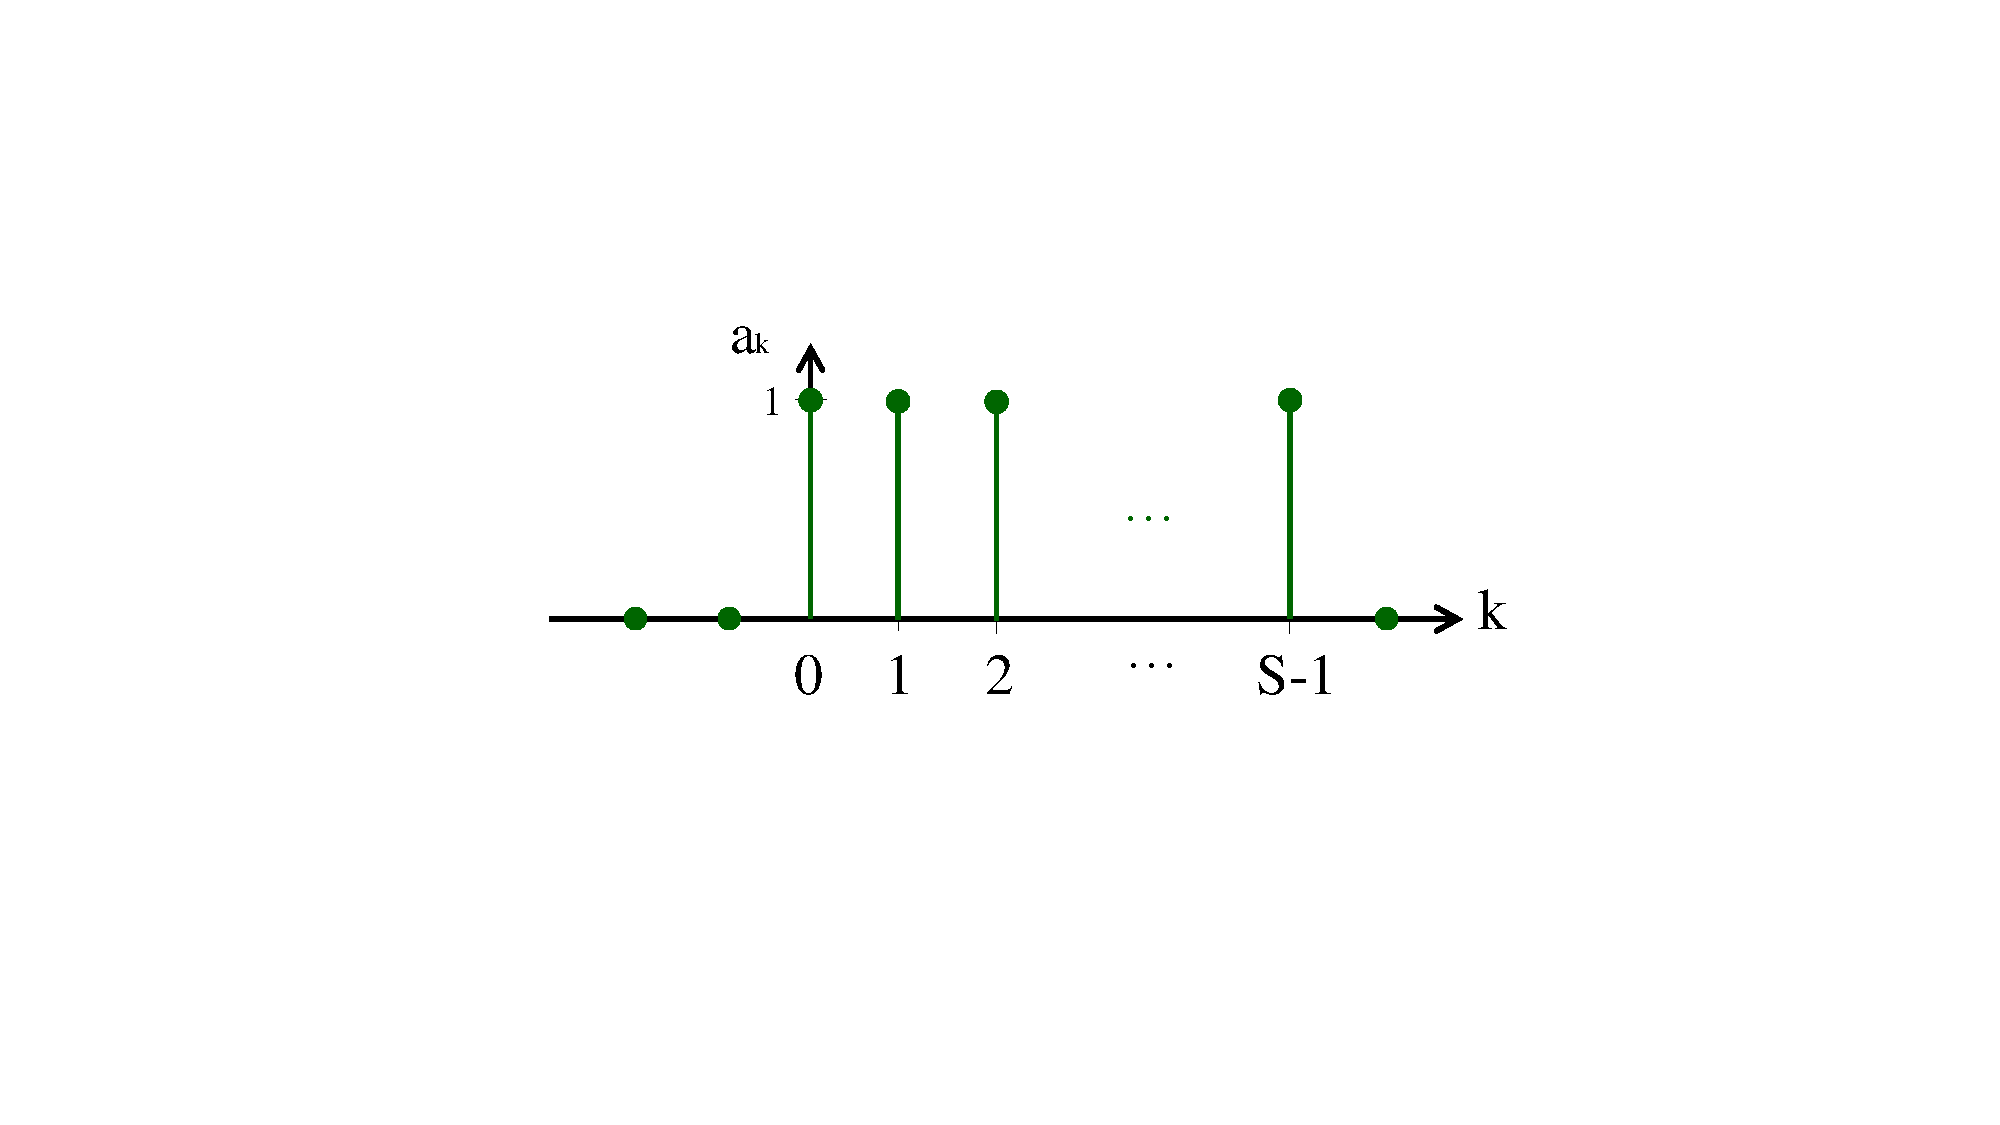
\includegraphics[trim =4cm 7cm 5cm 4cm, clip, width=0.70\textwidth]{graphics/SDP_square_window.pdf}
	\caption{Square window weighting}
	\label{fig:SDP_square_window}
\end{figure}
The weighting coefficients  $a_k$ can be chosen in different ways. One may be to do a square window weighting (see figure \ref{fig:SDP_square_window}), where in total $S$ previous values of $\vec{u}$ are taken into account and weighted equally (moving average). But usually it is better to weight the older values less than newer ones. Therefor an exponential weighting  is used commonly.\\
\mybox{
\textbf{Exponential weighting (Exponential Window):} $a_k=\eta^k;\quad |\eta|\leq 1$
}\\

\begin{doublespace}
$\ma{\hat{R}}[n]=\frac{\sum\limits_{k=0}^{\infty}\eta^k\vec{u}[n-k]\vec{u}^H[n-k]}{\underbrace{\sum\limits_{k=0}^{\infty}\eta^k}_{\frac{1}{1-\eta}}}$\\
To simplify the implementation of the calculation a recursive equation should be derived:\\
$\ma{\hat{R}}[n]=(1-\eta)\sum\limits_{k=0}^{\infty}\eta^k\vec{u}[n-k]\vec{u}^H[n-k]$\\
\begin{flalign*}
\ma{\hat{R}}[n+1]&=(1-\eta)\sum\limits_{k=0}^{\infty}\eta^k\vec{u}[n+1-k]\vec{u}^H[n+1-k]&&\\
&=(1-\eta)\sum\limits_{k+1=0}^{\infty}\eta^{k+1}\vec{u}[n-k]\vec{u}^H[n-k]&&\\
&=(1-\eta)\eta\sum\limits_{k=-1}^{\infty}\eta^{k}\vec{u}[n-k]\vec{u}^H[n-k]&&\\
&=\eta\underbrace{(1-\eta)\sum\limits_{k=0}^{\infty}\eta^{k}\vec{u}[n-k]\vec{u}^H[n-k]}_{\ma{\hat{R}}[n]} + (1-\eta)\underbrace{\eta\eta^{-1}}_{1}\vec{u}[n+1]\vec{u}^H[n+1]
\end{flalign*}
\mybox{
$\ma{\hat{R}}[n+1]=\eta\ma{\hat{R}}[n] + (1-\eta)\vec{u}[n+1]\vec{u}^H[n+1]$
}
$\vec{\hat{p}}[n+1]=\eta\vec{\hat{p}}[n](1-\eta)\vec{u}[n+1]d^*[n+1]$\\ \\
\mybox{
\textbf{SDP (Steepest Descent Procedure):}\\
\pfeil with optimal step size and estimation of correlation matrix and correlation vector\\
\pfeil procedure never stops. \\
\textbf{Input:} $\vec{u}[n],\quad d[n]$\\
\textbf{Output:} sequence of $\vec{w}[n]$\\
\begin{tabular}{ll}
	1. Init: &$\ma{\hat{R}}\leftarrow\ma{0},\quad\vec{\hat{p}}\leftarrow \vec{0},\quad \vec{w}\leftarrow \vec{0},\quad n\leftarrow0$\\
	2. Estimation: &$\ma{\hat{R}}\leftarrow\eta\ma{\hat{R}}+(1-\eta)\vec{u}[n+1]\vec{u}^H[n+1]$\\
	&$\vec{\hat{p}}\leftarrow \eta\vec{\hat{p}}[n](1-\eta)\vec{u}[n+1]d^*[n+1]$\\
  3. Weight update: &$\vec{\hat{r}}\leftarrow\vec{\hat{p}}-\ma{\hat{R}}\vec{w}$\\
	&$\hat{\mu}\leftarrow\frac{\vec{\hat{r}}^H\vec{\hat{r}}}{\vec{\hat{r}}H\ma{\hat{R}}\vec{\hat{r}}}$\\
	&$\vec{w}\leftarrow\vec{w}\hat{\mu}\vec{\hat{r}}$\\
	4. Output \vec{w} for $\vec{w}[n+1]$&\\
	5. $n\leftarrow n+1$, go to step 2&\\
\end{tabular}}\\
\textbf{Note:} This is called procedure and not algorithm since an algorithm needs to stop (finish) after a finite time (by definition). That's not the case here.\\
\begin{figure}[H]
	\centering
		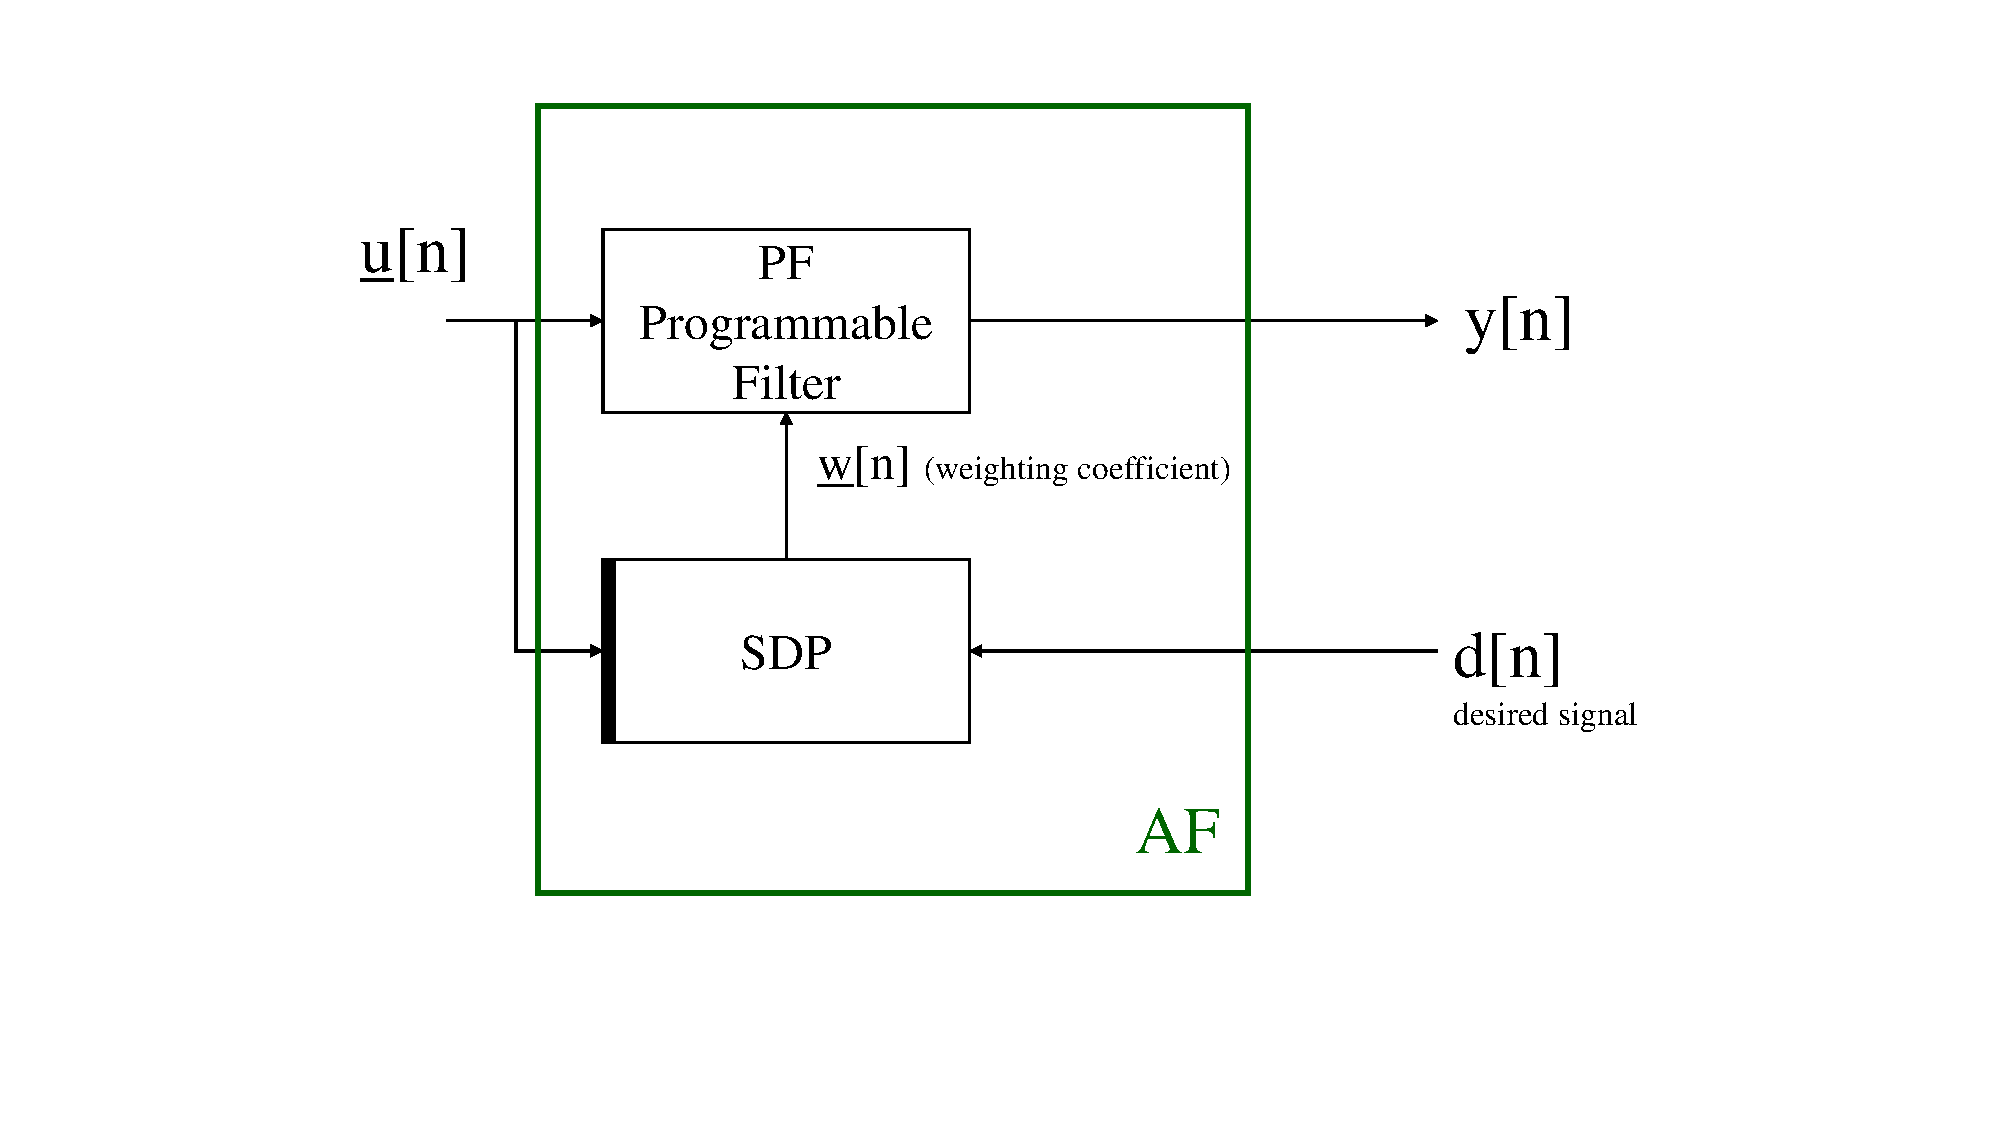
\includegraphics[trim =4cm 3cm 4cm 1cm, clip, width=0.70\textwidth]{graphics/adaptive_filter_with_SDP.pdf}
	\caption{Block diagram of an adaptive filter (AF) using the ``Steepest Descent Procedure''}
	\label{fig:adaptive_filter_with_SDP}
\end{figure}

\begin{tabular}{ll}
\textbf{Note:}&$\eta$ close to 0:\\
&$\quad$ Pro: Track fast changing channels better\\
&$\quad$ Con: Poor estimation for slow changing channels\\
&\\
&$\eta$ close to 1:\\
&$\quad$ Pro: Good estimation for slow changing channels\\
&$\quad$ Con: Bad tracking of fast changing channels\\
&\\
\end{tabular}

\textbf{Note: LMS-Procedure:}\\
$\text{``LMS''}=\lim\limits_{\eta\rightarrow 0}\text{``SDP''}$\\
$\ma{\hat{R}}[n+1]=\vec{u}[n]\vec{u}^H[n], \quad \vec{\hat{p}}[n]=\vec{u}[n]d^*[n]$\\
$\vec{w}[n+1]=\vec{w}[n]+\mu\vec{u}[n]\vec{e}^*[n]$\\
$\vec{e}[n]=d[n]-\vec{w}^H[n]\vec{u}[n]$\\
$\mu=\frac{1}{||\vec{u}[n]||_2^2+a};\qquad a>0$\\
or $\mu=\const$\\
\rule{\textwidth}{0.4pt}

\textbf{Application: linearly constraint minimum variance problem}

$y[n]=\vec{w}^H\vec{u}[n]$\\
$\min \underbrace{E[|y[n]|^2]}_{\vec{w}^H \underbrace{E[\vec{u}[n]\vec{u}^H[n]]}_{\ma{R}=\ma{A}}\vec{w}}, \text{ s. t. } \ma{B}\vec{w}=\vec{c}$\\
$\vec{w}=\vec{w}_q-\ma{V}_2\vec{w}_a$\\
$y[n]=\vec{w}_q^H\vec{u}[n]-\vec{w}_a^H\ma{V}_2\vec{u}[n]$\\

\begin{figure}[H]
	\centering
		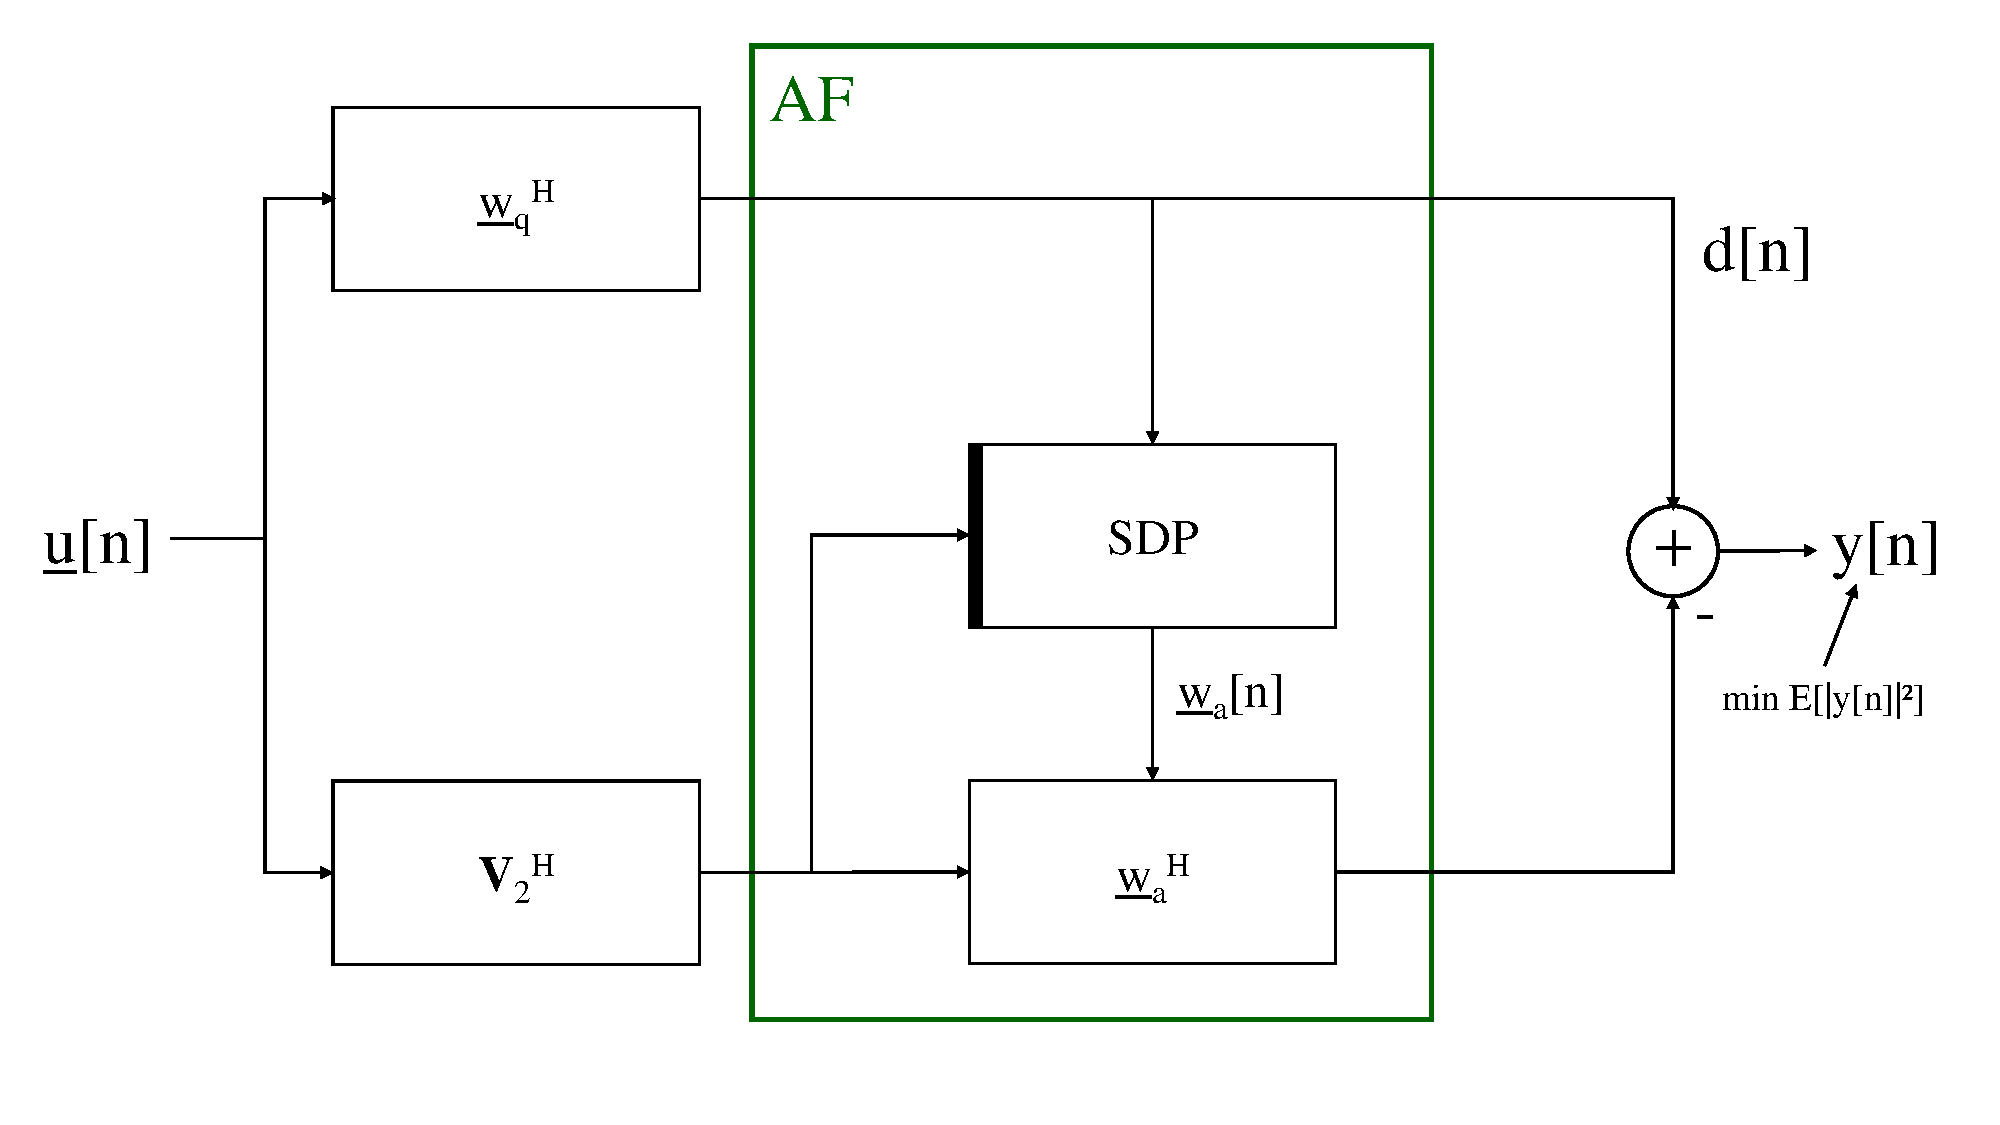
\includegraphics[trim =0cm 1.5cm 1cm 0cm, clip, width=1.00\textwidth]{graphics/Linearly_constraint_minimum_variance_problem.pdf}
	\caption{Linearly constraint minimum variance problem}
	\label{fig:Linearly_constraint_minimum_variance_problem}
\end{figure}
\end{doublespace}

\subsubsection{Example: Digital Spectrum Analyser (linear)}\label{sssec:dsa}
\begin{doublespace}
$u[n]=\sum\limits_{k=1}^{d}s_k \cdot e^{j2\pi f_k T n}+\nu[n]$\\
With following variables:\\
\begin{tabular}{rl}
$d$:& number of complex sinusoids\\
$f_1,\,f_2\,\ldots\,f_d$:& frequencies\\
$|s_1|,\,|s_2|\,\ldots\,|s_d|$:&amplitudes\\
$\arg S_1,\,\arg S_2,\,\ldots\,\arg S_d$:& phase\\
$T$:& sampling time\\
$\nu[n]$:& noise\\
\end{tabular}
 
We want to know: $d,\,f_1,\,f_2,\,\ldots\,f_d,\,|s_1|,\,|s_2|\,\ldots\,|s_d|$\\
\begin{flalign*}
\vec{u}[n]&=\mat{u[n]\\u[n-1]\\\svdots\\u[n-(M-1)]}=\mat{\sum\limits_{k=1}^{d}s_k \cdot e^{j2\pi f_k T\cdot n}+\nu[n]\\\sum\limits_{k=1}^{d}s_k \cdot e^{j2\pi f_k T \cdot (n-1)}+\nu[n-1]\\\svdots\\\sum\limits_{k=1}^{d}s_k \cdot e^{j2\pi f_k T\cdot (n-(M-1))}+\nu[n-(M-1)]}&&\\
&=\sum\limits_{k=1}^{d}s_k\underbrace{\mat{1\\e^{-j2\pi f_k T}\\\svdots\\e^{-(M-1)j2\pi f_k T}}}_{\vec{a}(f_k)}e^{j2\pi f_k T\cdot n}+\mat{\nu[n]\\\nu[n-1]\\\svdots\\\nu[n-(M-1)]}
\end{flalign*}
\mybox{
$\vec{u}[n]=\sum\limits_{k=1}^{d}s_k\vec{a}(f_k)e^{j2\pi f_k T n}+\vec{\nu}[n]$\\
}

\begin{figure}[H]
	\centering
		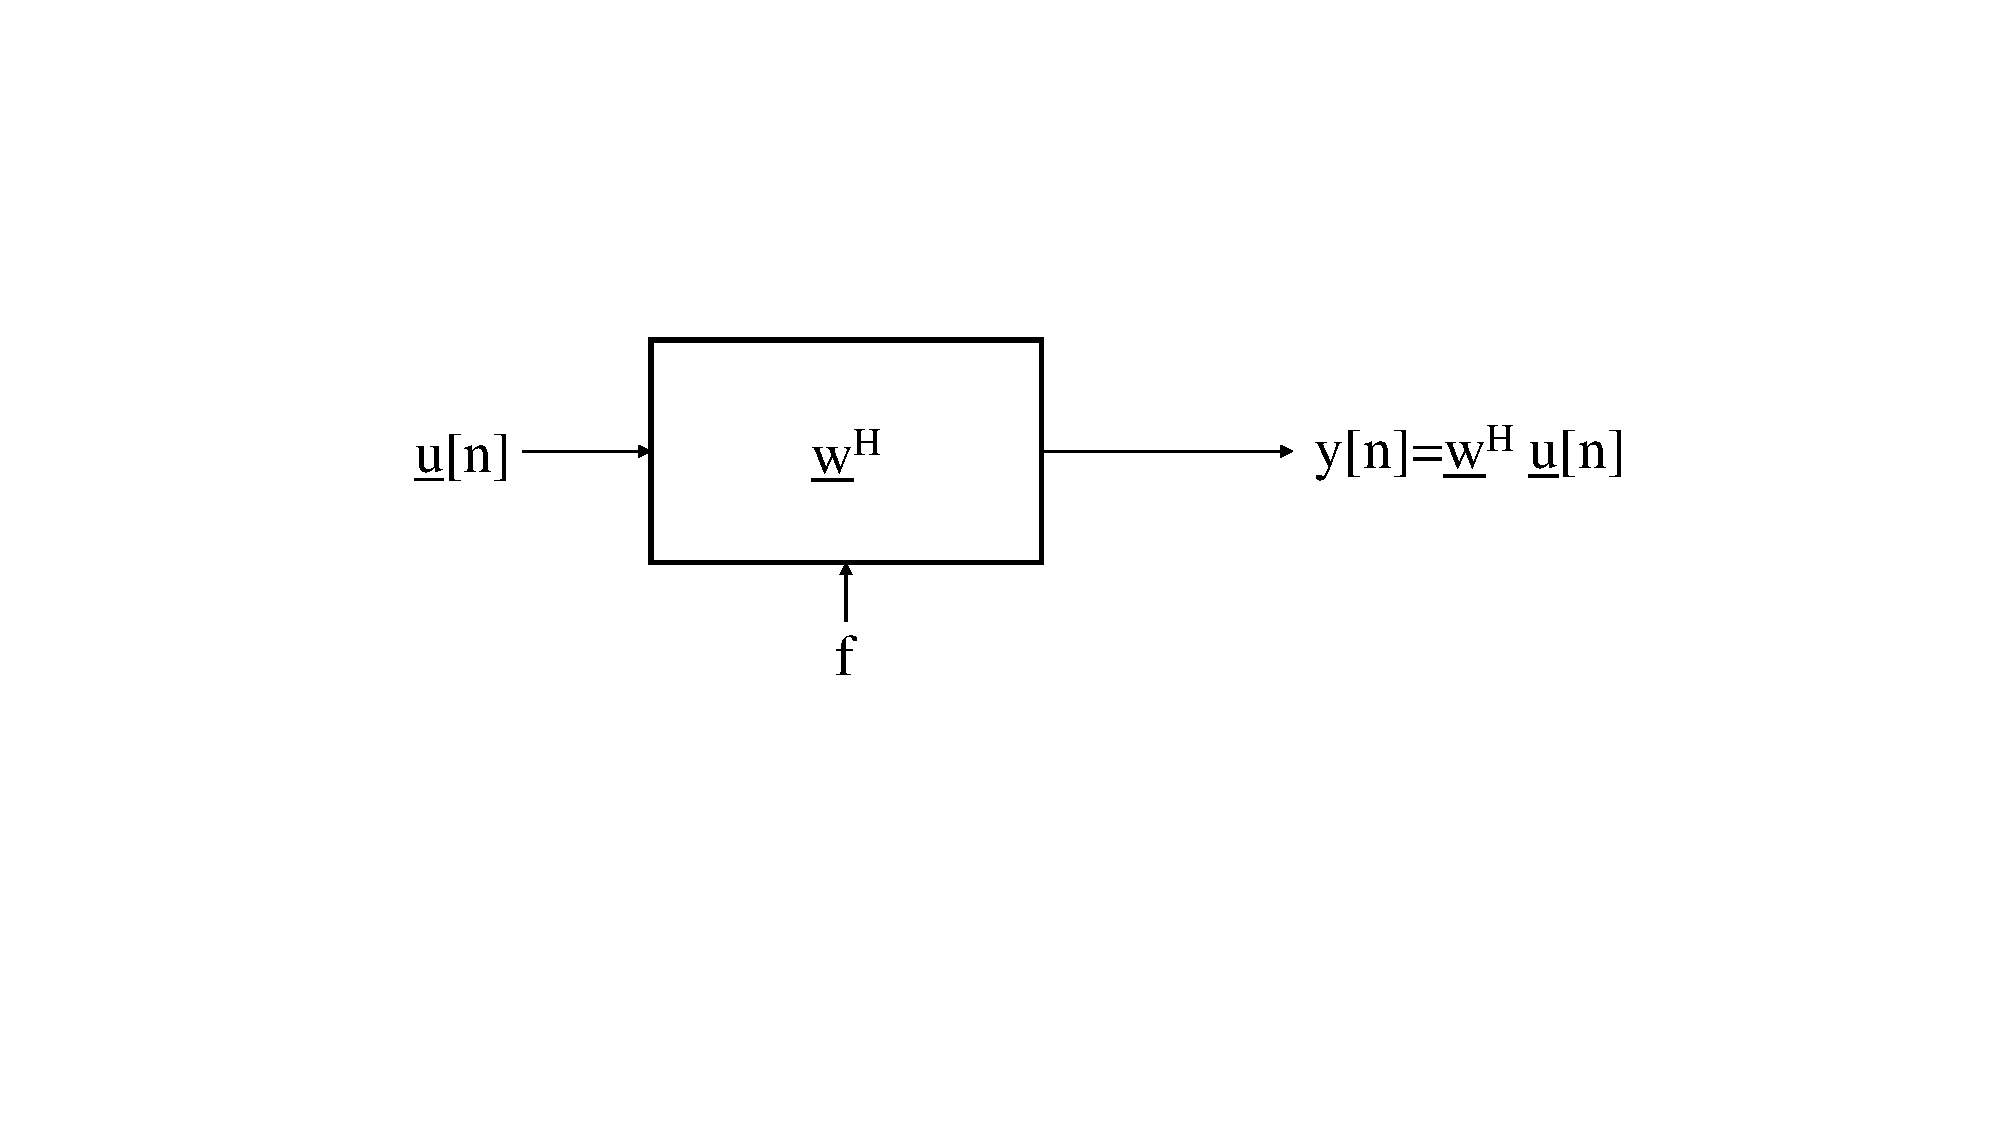
\includegraphics[trim =3cm 7cm 3cm 3cm, clip, width=0.70\textwidth]{graphics/ex_spectrum_analyzer.pdf}
	\caption{Block diagram of a Digital Spectrum Analyzer}
	\label{fig:ex_spectrum_analyzer}
\end{figure}

\begin{enumerate}
	\item $\vec{w}^H\vec{a}(f)=1\qquad \text{or } \underbrace{\vec{a}^H(f)}_{\ma{B}}\vec{w}=1$
	\item $\min \underbrace{E[|y[n]|^2]}_{\vec{w}^H\underbrace{E[\vec{u}[n]\vec{u}^H[n]]}_{\ma{A}}\vec{w}}$
\end{enumerate}
$\mathcal{L}=\vec{w}^H\ma{A}\vec{w}+\lambda(\vec{a}^H(f)\vec{w}-1)+(\vec{w}^H\vec{a}(f)-1)\lambda^*$\\
\mybox{
$\vec{w}_{opt}=\frac{\ma{A}^{-1}\vec{a}(f)}{\vec{a}^H(f)\ma{A}^{-1}\vec{a}(f)}$
}\\
$E[|y[n]|^2]=\vec{w}_{opt}^H\ma{A}\vec{w}_{opt}=\frac{1}{\vec{a}^H(f)\ma{A}^{-1}\vec{a}(f)}$\\ \ \\

$d=2,\quad M=3,\quad \sigma_\nu^2=0.001$\\
$S_1=1+j,\quad S_2=-1+2j,\quad T=0.25\,\mu\text{S}$\\
$|S_1|^2=2,\quad |S_2|^2=5$\\
$f_1=1\,\text{MHz},\quad f_2=1.7\,\text{MHz}$\\
Parameter: $\vec{a}(f_1)=\mat{1\\e^{-j2\pi f_1 T}\\e^{-j4\pi f_1 T}}\qquad \vec{a}(f_2)=\mat{1\\e^{-j2\pi f_2 T}\\e^{-j4\pi f_2 T}}$\\
Variable:\quad $\vec{a}(f)=\mat{1\\e^{-j2\pi f T}\\e^{-j4\pi f T}}$\\

\begin{flalign*}
\ma{A}&=E[\vec{u}[n]\vec{u}^H[n]]&&\\
&=|S_1|^2\vec{a}_1\vec{a}_1^H+|S_2|^2\vec{a}_2\vec{a}_2^H+0.001\ma{I}+S_1S_2^*e^{j2\pi(f_1-f_2)T n}+S_1^*S_2e^{-j2\pi(f_1-f_2)T n}
\end{flalign*}
$\ma{A}\leftarrow \underbrace{\ma{\bar{A}}}_{\text{time average}}=|S_1|^2\vec{a}_1\vec{a}_1^H+|S_2|^2\vec{a}_2\vec{a}_2^H+0.001\ma{I}$\\
$A_{11}=A_{22}=A_{33}=7.001$\\
$A_{21}=A_{32}=A_{12}^*=A_{23}^*=-4.455-j\,4.27$\\
$A_{31}=A_{13}^*=0.9389+j\,4.0451$\\


\begin{align*}
\ma{A}=&E[\vec{u}[n]\vec{u}^H[n]]=E\left[\left(\sum\limits_{k=1}^{2}s_k\vec{a}(f_k)e^{j2\pi f_k T n}+\vec{\nu}[n]\right)\left(\sum\limits_{k=1}^{2}s_k\vec{a}(f_k)e^{j2\pi f_k T n}+\vec{\nu}[n]\right)^H\right]\\
=&E\left[\left(s_1\vec{a}(f_1)e^{j2\pi f_1 T n}+s_2\vec{a}(f_2)e^{j2\pi f_2 T n}+\vec{\nu}[n]\right)
\left(s_1^*\vec{a}(f_1)^He^{-j2\pi f_1 T n}+s_2^*\vec{a}(f_2)^He^{-j2\pi f_2 T n}+\vec{\nu}[n]^H\right)\right]\\
=&\abs{s_1}\vec{a}_1\vec{a}_1^H+\abs{s_2}\vec{a}_2\vec{a}_2^H+\sigma_\nu^2\ma{I}+s_1s_2^*\vec{a}(f_1)\vec{a}(f_2)^He^{j2\pi (f_1-f_2) T n}+
s_2s_1^*\vec{a}(f_2)\vec{a}(f_1)^He^{j2\pi (f_2-f_1) T n}
\end{align*}

$\ma{\bar{A}}=\mat{7.001&-4.455+\j 4.27&0.9389-\j 4.0451\\-4.455-\j 4.27&7.001&-4.455+\j 4.27\\ 0.9389+\j 4.0451 & -4.455-\j 4.27 & 7.001}$

$\ma{\bar{A}}^{-1}=100\cdot\mat{2.0858&1.8569-\j 3.0297&-0.9460-\j 1.8553\\1.8569+\j 3.0297&6.0603&1.8569-\j 3.0297\\ -0.9460+\j 1.8553 & 1.8569+\j 3.0297 & 2.0858}$

\begin{figure}[H]
	\centering
		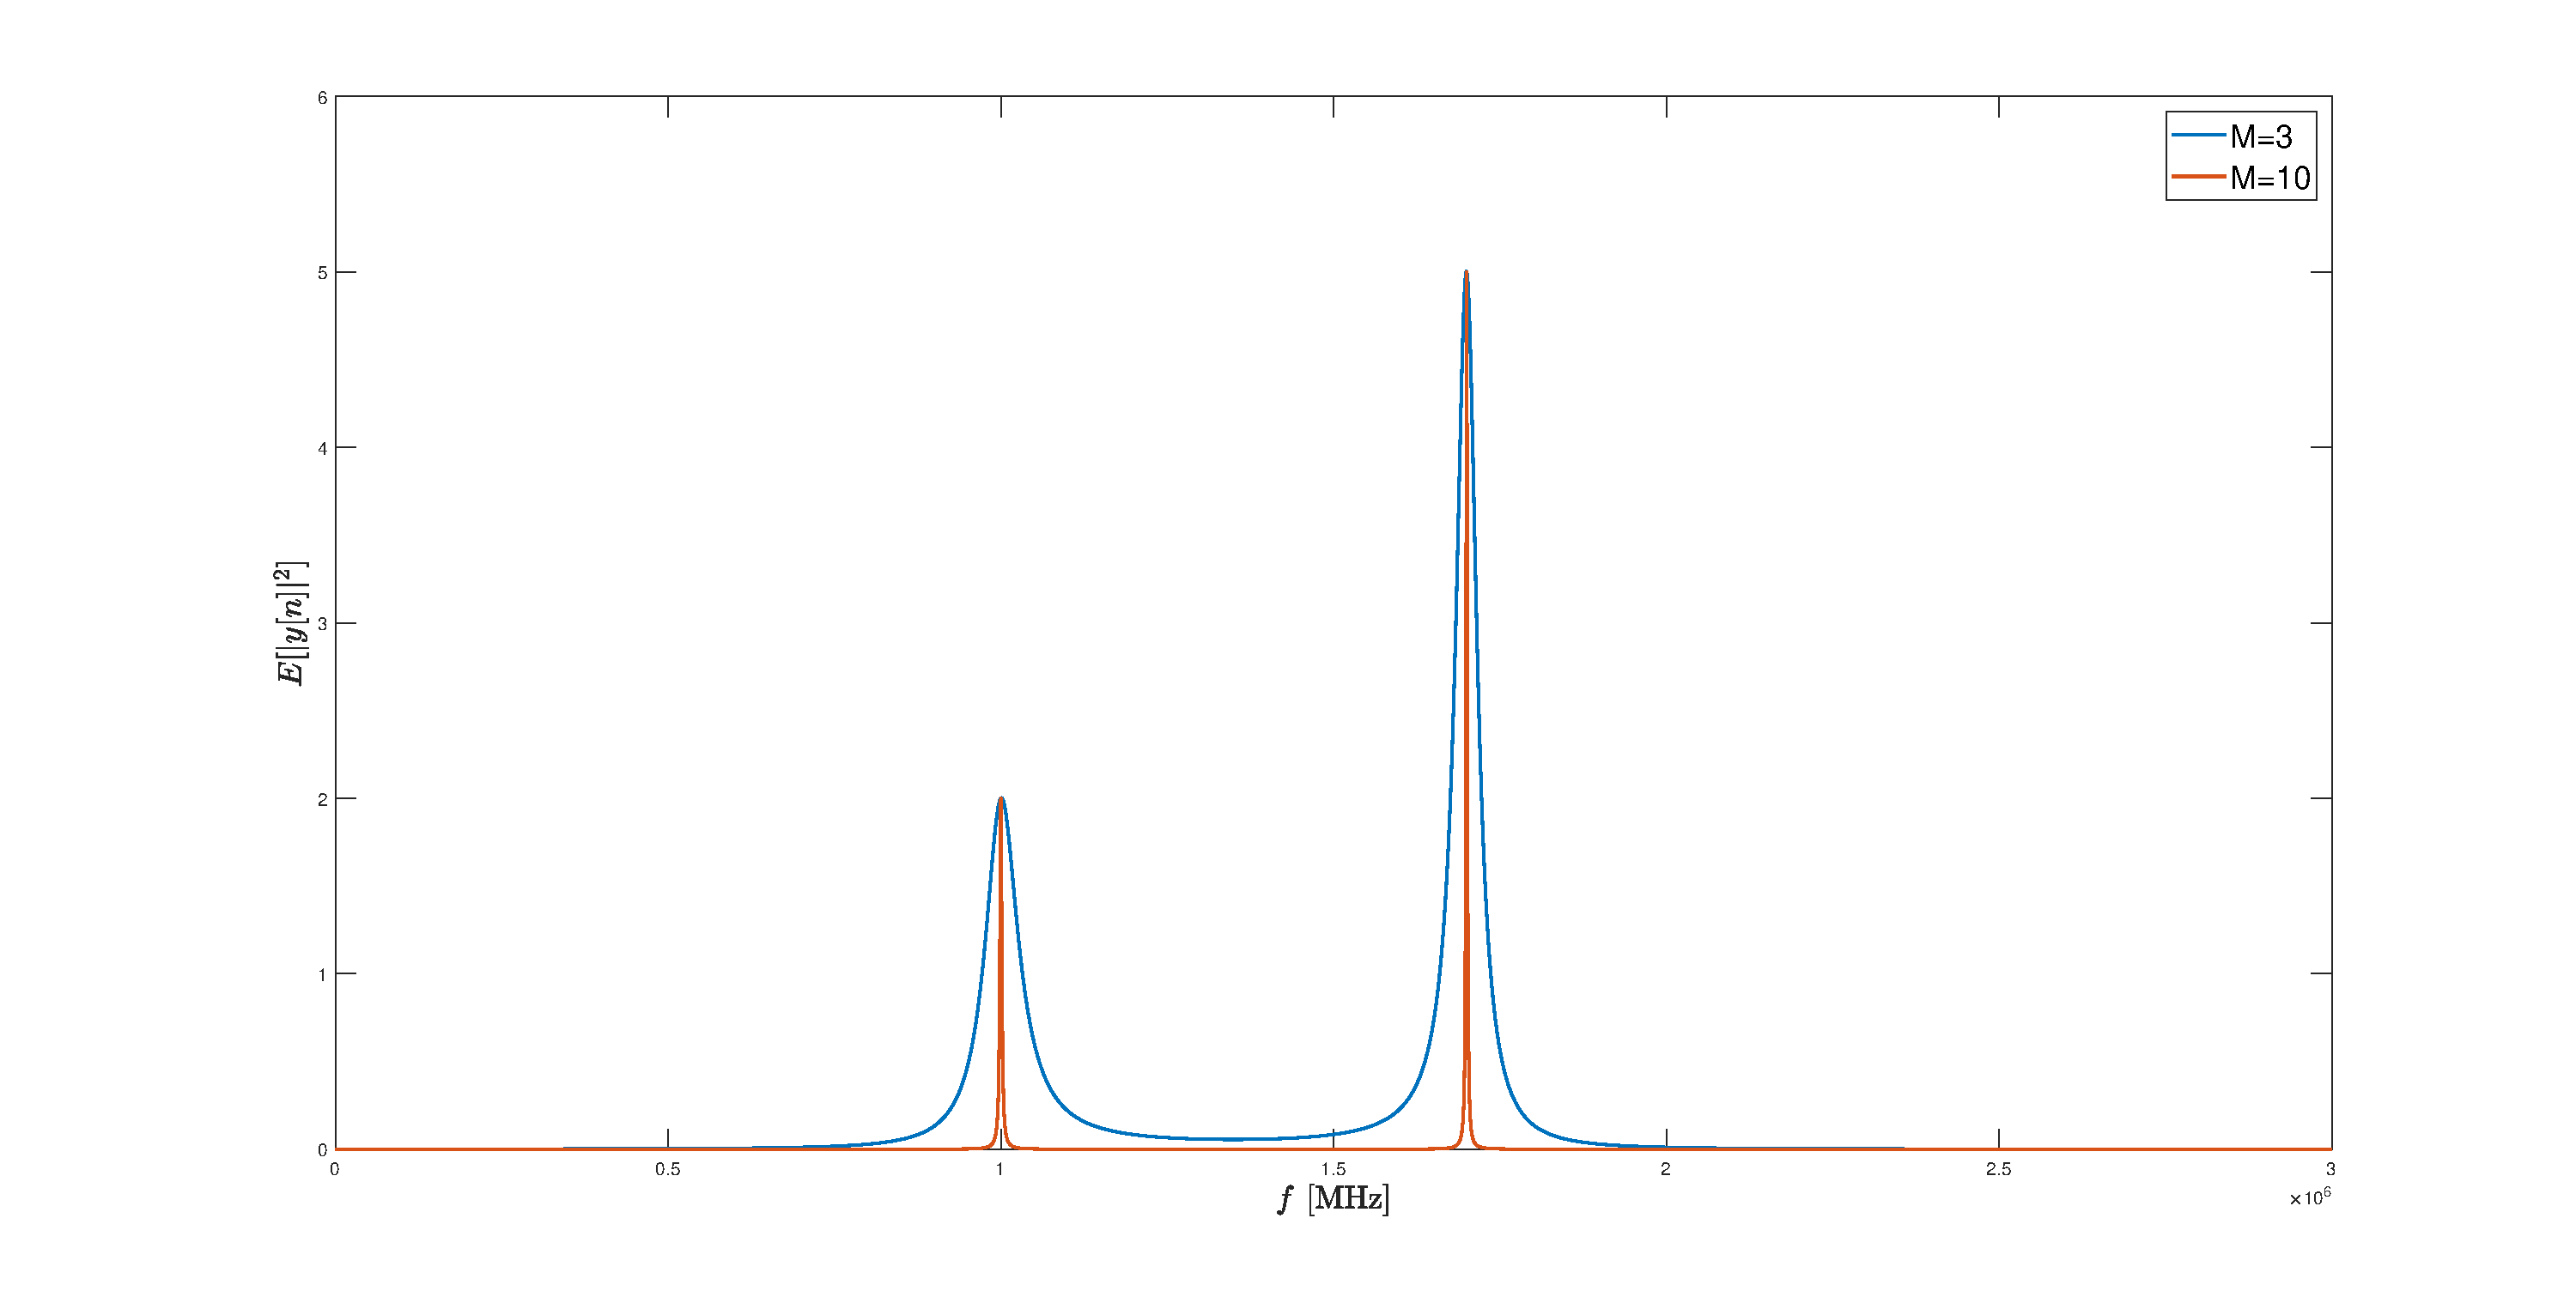
\includegraphics[trim =4cm 1cm 4cm 1cm, clip, width=1.00\textwidth]{graphics/ex_spectrum_analyzer_result_plot.pdf}
	\caption{Plot of the result for two difference memory depth ($M=3$ and $M=10$)}
	\label{fig:ex_spectrum_analyzer_result_plot}
\end{figure}

\end{doublespace}


\newpage
\section{Spatial Filtering}
\begin{doublespace}
\begin{figure}[htbp]
	\centering
		\includegraphics[trim =6cm 7cm 6cm 4cm, clip,width=0.70\textwidth]{graphics/Spatial_filtering_antenna_example.pdf}
	\caption{Eaxample of a spatial filtering scenario: Sender with 1 antenna and Receiver with 3 antennas (as ULA)}
	\label{fig:SPatial_filtering_antenna_example}
\end{figure}
$\vec{x}[n]=\mat{x_1[n]\\x_2[n]\\\svdots\\x_M[n]}=\sum\limits_{k=1}^{d}\vec{a}(\Theta_k)s_k[n]+\vec{\nu}[n]$\\
$\vec{a}(\Theta)=\mat{1\\e^{-j2\pi \frac{\Delta}{\lambda} \cos(\Theta)}\\e^{-j 2 \cdot 2\pi \frac{\Delta}{\lambda} \cos(\Theta)}\\\svdots\\e^{-j(M-1)2\pi \frac{\Delta}{\lambda} \cos(\Theta)}}$\\
$\vec{x}[n]=\underbrace{\mat{\vec{a}(\Theta_1)&\vec{a}(\Theta_2)&\shdots&\vec{a}(\Theta_d)}}_{\ma{A}\in\mathbb{C}^{M\times d}}\cdot\underbrace{\mat{s_1[n]\\s_2[n]\\\svdots\\s_d[n]}}_{\vec{s}[n]\in\mathbb{C}^{M\times 1}}+\underbrace{\vec{\nu}}_{\in\mathbb{C}^{M\times 1}}$\\
$\vec{x}[n]=\ma{A}\cdot \vec{s}[n]+\vec{\nu}[n]$\\
With:\\
\begin{tabular}{rl}
$\vec{x}[n]$: & Observation Snapshot\\
$\ma{A}$: & Steering Matrix\\
$\vec{s}[n]$: & Signal Vector\\
$\vec{\nu}[n]$:& Noise\\
\end{tabular}\\ \\
\textbf{Observation Matrix (Space/time):}\\
$\ma{X}:=\mat{\vec{x}[n]&\vec{x}[n+1]&\shdots&\vec{x}[n+N-1]}\in\mathbb{C}^{M\times N}$\\
$\ma{S}:=\mat{\vec{s}[n]&\vec{s}[n+1]&\shdots&\vec{s}[n+N-1]}\in\mathbb{C}^{d\times N}$\\
$\ma{\nu}:=\mat{\vec{\nu}[n]&\vec{\nu}[n+1]&\shdots&\vec{\nu}[n+N-1]}\in\mathbb{C}^{M\times N}$\\
N snapshots\\
\mybox{
$\ma{X}=\ma{A}\ma{S}+\ma{\nu}$
}\\  \\
\begin{tabular}{ll}
\underline{Given:}&\ma{X} and \ma{A}\\
&and possibly $2^{nd}$-order statistics of \ma{S} and/or $\ma{\nu}$\\
\underline{Find:}&Estimate $\ma{\hat{S}}$ of \ma{S}\\
\underline{Here:}&Linear estimations $\ma{\hat{S}}=\ma{W}^H\ma{X}$\\
\end{tabular}
\end{doublespace}

\subsection{Case 1: Only X and A are known - Least Square}
\begin{doublespace}
Idea: $\ma{X}\approx\ma{A}\ma{S}\qquad$ (we assume that \ma{\nu} is small)\\
$\ma{\hat{S}}=\arg \min\limits_{\ma{S}}||\ma{X}-\ma{A}\ma{S}||_F^2$\\
$\rightarrow$ Least squares solution\\
\begin{flalign*}
||\ma{B}||_F^2=\sum\limits_{n,m}|B_{n,m}|^2=\sum\limits_{k=1}^{M}\vec{b}_k^H\vec{b}_k=\sum\limits_{k=1}^{M}\abs{\abs{\vec{b}_k}}_2^2=\trace\ma{B}^H\ma{B}
=\trace \mat{\vec{b}_1^H\\\vec{b}_2^H\\\svdots}\mat{\vec{b}_1&\vec{b}_2&\shdots}=\vec{b}_1^H\vec{b}_1+\vec{b}_2^H\vec{b}_2+\shdots
\end{flalign*}
Frobenius norm of the error:
\begin{flalign*}
\varepsilon &= ||\ma{X}-\ma{A}\ma{S}||_F^2=\trace\left((\ma{X}-\ma{A}\ma{S})^H(\ma{X}-\ma{A}\ma{S})\right)
=\trace\left((\ma{X}^H-\ma{S}^H\ma{A}^H)(\ma{X}-\ma{A}\ma{S})\right)&&\\
&=\trace(\ma{X}\ma{X}^H)-\trace(\ma{X}^H\ma{A}\ma{S})-\trace(\ma{S}^H\underbrace{\ma{A}^H\ma{X}}_{\ma{B}})+\trace(\ma{S}^H\ma{A}^H\ma{A}\ma{X})
\end{flalign*}

\mybox{
\textbf{Definition}:  Derivation of a scalar fuction with respect to a matrix:\\
$\frac{\partial \varepsilon}{\partial \ma{S}^*}:=\mat{\frac{\partial \varepsilon}{\partial \vec{S}_1^*}&\frac{\partial \varepsilon}{\partial \vec{S}_2^*}&\shdots&\frac{\partial \varepsilon}{\partial \vec{S}_N^*}}$}\\
\ \\

\with substitution: $\ma{A}^H\ma{X}=\ma{B}$\\

$\frac{\partial\trace(\ma{S}^H\ma{B})}{\partial\vec{s}_i^*}=\frac{\partial\trace \mat{\vec{s}_1^H\\\svdots\\\vec{s}_N^H}\mat{\vec{b}_1&\shdots&\vec{b}_N}}{\partial\vec{s}_i^*}=\frac{\vec{s}_1^H\vec{b}_1+\ldots+\vec{s}_N^H\vec{b}_N}{\partial\vec{s}_i^*}=\vec{b}_i$\\ \\
$\frac{\partial\trace(\ma{S}^H\ma{B})}{\partial\ma{S}^*}=\mat{\vec{b}_1&\vec{b}_2&\shdots&\vec{b}_N}=\ma{B}$\\ 
$\frac{\partial\varepsilon}{\partial\ma{S}^H}=-\ma{A}^H\ma{X}+\ma{A}^H\ma{A}\ma{S}\stackrel{!}{=}\ma{0}$\\
\mybox{
$\ma{\hat{S}}_{LS}=(\ma{A}^H\ma{A})^{-1}\ma{A}^H\ma{X}=\ma{A}^+\ma{X}=\ma{W}^H\ma{X}$
}\\
$\ma{A}\in\mathbb{C}^{M\times d}$\\
$\ma{A}^H\ma{A}\in\mathbb{C}^{d\times d},\quad$ Assume $\rank \ma{A}=d$ \qquad \pfeil Number of incoming wavefronts: $d$\\
$\rank\ma{A}^H\ma{A}=\rank\ma{A}=d$\\
$\Rightarrow$ all $d$ steering vectors $\vec{a}(\Theta_1)\ldots\vec{a}(\Theta_d)$ are L.I.D.\\ \ \\
\textbf{Calculation with realistic signal (Add observation noise) }\\
$\ma{X}=\ma{A}\ma{S}+\ma{\nu}$\\
$\ma{\hat{S}_{LS}}=(\ma{A}^H\ma{A})^{-1}\ma{A}^H(\ma{A}\ma{S}+\ma{\nu})$\\
$\ma{\hat{S}_{LS}}=\underbrace{(\ma{A}^H\ma{A})^{-1}\ma{A}^H\ma{A}}_{\ma{I}}\ma{S}+(\ma{A}^H\ma{A})^{-1}\ma{A}^H\ma{\nu}$\\
\mybox{
$\ma{\hat{S}_{LS}}=\ma{S}+\underbrace{(\ma{A}^H\ma{A})^{-1}\ma{A}^H\ma{\nu}}_{\text{Estimation Noise}}$\\
$\ma{\nu}$: Observation Noise
}\\ \ \\
Note: Mean value:\\
$E[\ma{\hat{S}_{LS}}]=E[\ma{S}]+(\ma{A}^H\ma{A})^{-1}\ma{A}^H\underbrace{E[\ma{\nu}]}_{=0}=E[\ma{S}]$\\
$\Rightarrow$ \underline{unbiased} estimate, because the arithmetic mean value of the noise is zero

\subsubsection{Signal-to-Noise Ratio (SNR)}
\begin{flalign*}
SNR&=\frac{E[||\ma{\hat{S}}_{LS}||_F^2\left.\right|\ma{\nu}=0]}{E[||\ma{\hat{S}}_{LS}||_F^2\left.\right|\ma{S}=0]}
=\frac{E[||\ma{S}||_F^2]}{E[||(\ma{A}\ma{A}^H)^{-1}\ma{\nu}||_F^2]}
=\frac{E[\trace\ma{S}^H\ma{S}]}{E[\trace\ma{A}^+\ma{\nu}\ma{\nu}^H(\ma{A}^+)^H]}
=\frac{\trace E[\ma{S}^H\ma{S}]}{\trace E[\ma{A}^+\ma{\nu}\ma{\nu}^H(\ma{A}^+)^H]}&&\\
&=\frac{\trace E[\ma{S}^H\ma{S}]}{\trace (\ma{A}^+E[\ma{\nu}\ma{\nu}^H](\ma{A}^+)^H)}
\end{flalign*}
Numinator of SNR:
\begin{flalign*}
\trace E[\ma{S}^H\ma{S}]&=\trace E\left[\mat{\vec{s}^H[n]\\\vec{s}^H[n+1]\\\svdots\\\vec{s}^H[n+N-1]}\mat{\vec{s}[n]&\vec{s}[n+1]&\shdots&\vec{s}[n+N-1]}\right]&&\\
&=E\left[\trace(\vec{s}^H[n]\vec{s}[n])+\trace(\vec{s}^H[n+1]\vec{s}[n++1])+\ldots+\trace(\vec{s}^H[n+N-1]\vec{s}[n+N-1])\right]&&\\
&=E\left[\sum\limits_{k=0}^{N-1}\vec{s}^H[n+k]\vec{s}[n+1]\right]&&\\
&=N\cdot E[\vec{s}^H[n]\vec{s}[n]]&&\\
&=N\cdot E[\trace(\vec{s}^H[n]\vec{s}[n])]&&\\
&=N\cdot E[\trace(\vec{s}[n]\vec{s}^H[n])]&&\\
&=N\cdot \trace(\underbrace{E[\vec{s}[n]\vec{s}^H[n]]}_{\ma{R}_s})
\end{flalign*}
\pfeil Signal correlation matrix: $\ma{R}_s$
\\ \ \\
Interim results:\\
$ SNR=\frac{N\tr\ma{R}_s}{\trace(\ma{A}^+E[\ma{\nu}\ma{\nu}^H](\ma{A}^+)^H)}$\\
Denominator of SNR: 
\begin{flalign*}
E[\ma{\nu}\ma{\nu}^H]&=E\left[\mat{\vec{\nu}[n]&\vec{\nu}[n+1]&\shdots&\vec{\nu}[n+N-1]}\mat{\vec{\nu}^H[n]\\\vec{\nu}^H[n+1]\\\svdots\\\vec{\nu}^H[n+N-1]}\right]&&\\
&=E[\vec{\nu}[n]\vec{\nu}^H[n]+\vec{\nu}[n+1]\vec{\nu}^H[n+1]+\ldots+\vec{\nu}[n+N-1]\vec{\nu}^H[n+N-1]]&&\\
&=N \cdot \underbrace{E[\vec{\nu}[n]\vec{\nu}^H[n]]}_{\ma{R}_\nu}\qquad\text{Assume: Noise is stationary}
\end{flalign*}
\pfeil Noise correlation matrix: $\ma{R}_\nu$\\ \ \\
\mybox{
$SNR=\frac{\trace \ma{R}_s}{\trace(\ma{A}^+\ma{R}_\nu(\ma{A}^+)^H)}=\frac{\trace \ma{R}_s}{\trace((\ma{A}^H\ma{A})^{-1}\ma{A}^H\ma{R}_\nu\ma{A}(\ma{A}^H\ma{A})^{-1})}$\\
with: $\ma{A}^+=(\ma{A}^H\ma{A})^{-1}\ma{A}^H$
}\\ \ \\
\paragraph{Special case: White signal and white noise}
$\ma{R}_s=\sigma_s^2\ma{I}_d,\qquad$ white signal \pfeil $\tr(\ma{R})_s=d\cdot \sigma_s^2$\\
$\ma{R}_\nu=\sigma_\nu^2\ma{I}_M,\qquad$ white noise\\
$SNR=\frac{d\cdot \sigma_s^2}{\trace((\ma{A}^H\ma{A})^{-1}\ma{A}^H\sigma_\nu^2\ma{A}(\ma{A}^H\ma{A})^{-1})}=\frac{d\cdot\frac{\sigma_s^2}{\sigma_\nu^2}}{\trace(\ma{A}^H\ma{A})^{-1}}$\\
$\ma{A}^H\ma{A}\underbrace{=}_{\text{EVD}}\ma{Q}\ma{\Lambda}\ma{Q}^H;\qquad \ma{Q}^{-1}=\ma{Q}^H$\\
$(\ma{A}^H\ma{A})^{-1}=\ma{Q}\ma{\Lambda}^{-1}\ma{Q}^H$\\
$\trace(\ma{A}^H\ma{A})^{-1}=\trace(\ma{Q}\underbrace{\ma{\Lambda}^{-1}\ma{Q}^H}_{\ma{D}})=\trace(\ma{Q}^H\ma{Q}\ma{\Lambda}^{-1})=\trace\Lambda^{-1}$\\
\mybox{
$SNR=\frac{d\cdot\frac{\sigma_s^2}{\sigma_\nu^2}}{\sum\limits_{k=1}^d\frac{1}{\lambda_k}} \quad \with \lambda_k \textrm{ Eigenvalues of } \ma{A}^H\ma{A}$
}
\paragraph{Optimum case for LS with white noise and signal}
SNR is maximum for $\sum \frac{1}{\lambda_k}$ is minimum:\\
$\pfeil\sum\limits_{k=1}^d\frac{1}{\lambda_k}$ is minimum, s. t. $\sum\limits_{k=1}^d\lambda_k=c=\const$\\
$\sum\limits_{k=1}^d\lambda_k=\trace\Lambda=\trace\ma{A}^H\ma{A}=\sum\limits_{k=1}^d||\vec{a}(\Theta_1)||_2^2=M\cdot d$\\
$\mathcal{L}=\sum\limits_{k=1}^d\frac{1}{\lambda_k}+\underbrace{\mu}_{\text{Lagrange-multiplier}}(\sum\limits_{k=1}^d\lambda_k-c)$\\
$\frac{\partial\mathcal{L}}{\partial\lambda_i}=-\frac{1}{\lambda_i^2}+\mu\stackrel{!}{=}0;\qquad \lambda_i=\frac{1}{\sqrt{\mu}}$\\
$\lambda_1=\lambda_2=\ldots=\lambda_d=\frac{c}{d}=M$\\
\underline{Check if we found a minimum:}\\
$\sum\limits_{k=1}^d\frac{1}{\lambda_k}=\frac{1}{\frac{c}{d}+x}+\frac{1}{\frac{c}{d}-x}+\frac{d}{c}(d-2)$\\
Taylor-Series with respect to $x$ around $0$:\\
$\sum\limits_{k=1}^d\frac{1}{\lambda_k}=\frac{d^2}{c}+\underbrace{\frac{2d}{c}\sum\limits_{n=1}^\infty\underbrace{(\frac{d}{c}x)^{2n}}_{\geq0}}_{\geq 0}$\\
$\Rightarrow$ Minimum for $x=0\quad \Rightarrow$ maximum SNR\\
\underline{Alternative to show that it is a minimum:}\\
$\frac{d\frac{\sigma_s^2}{\sigma_\nu^2}}{\sum\limits_{k=1}^d\frac{1}{\lambda_k}}\leq d\frac{\sigma_s^2}{\sigma_\nu^2}\lambda_{min}$\\ \\

\mybox{
For white noise and white signal the Least-Squares-Estimation works best if and only if\\
$\ma{A}^H\ma{A}=\const\cdot\ma{I}$
}
\begin{figure}[H]
	\centering
		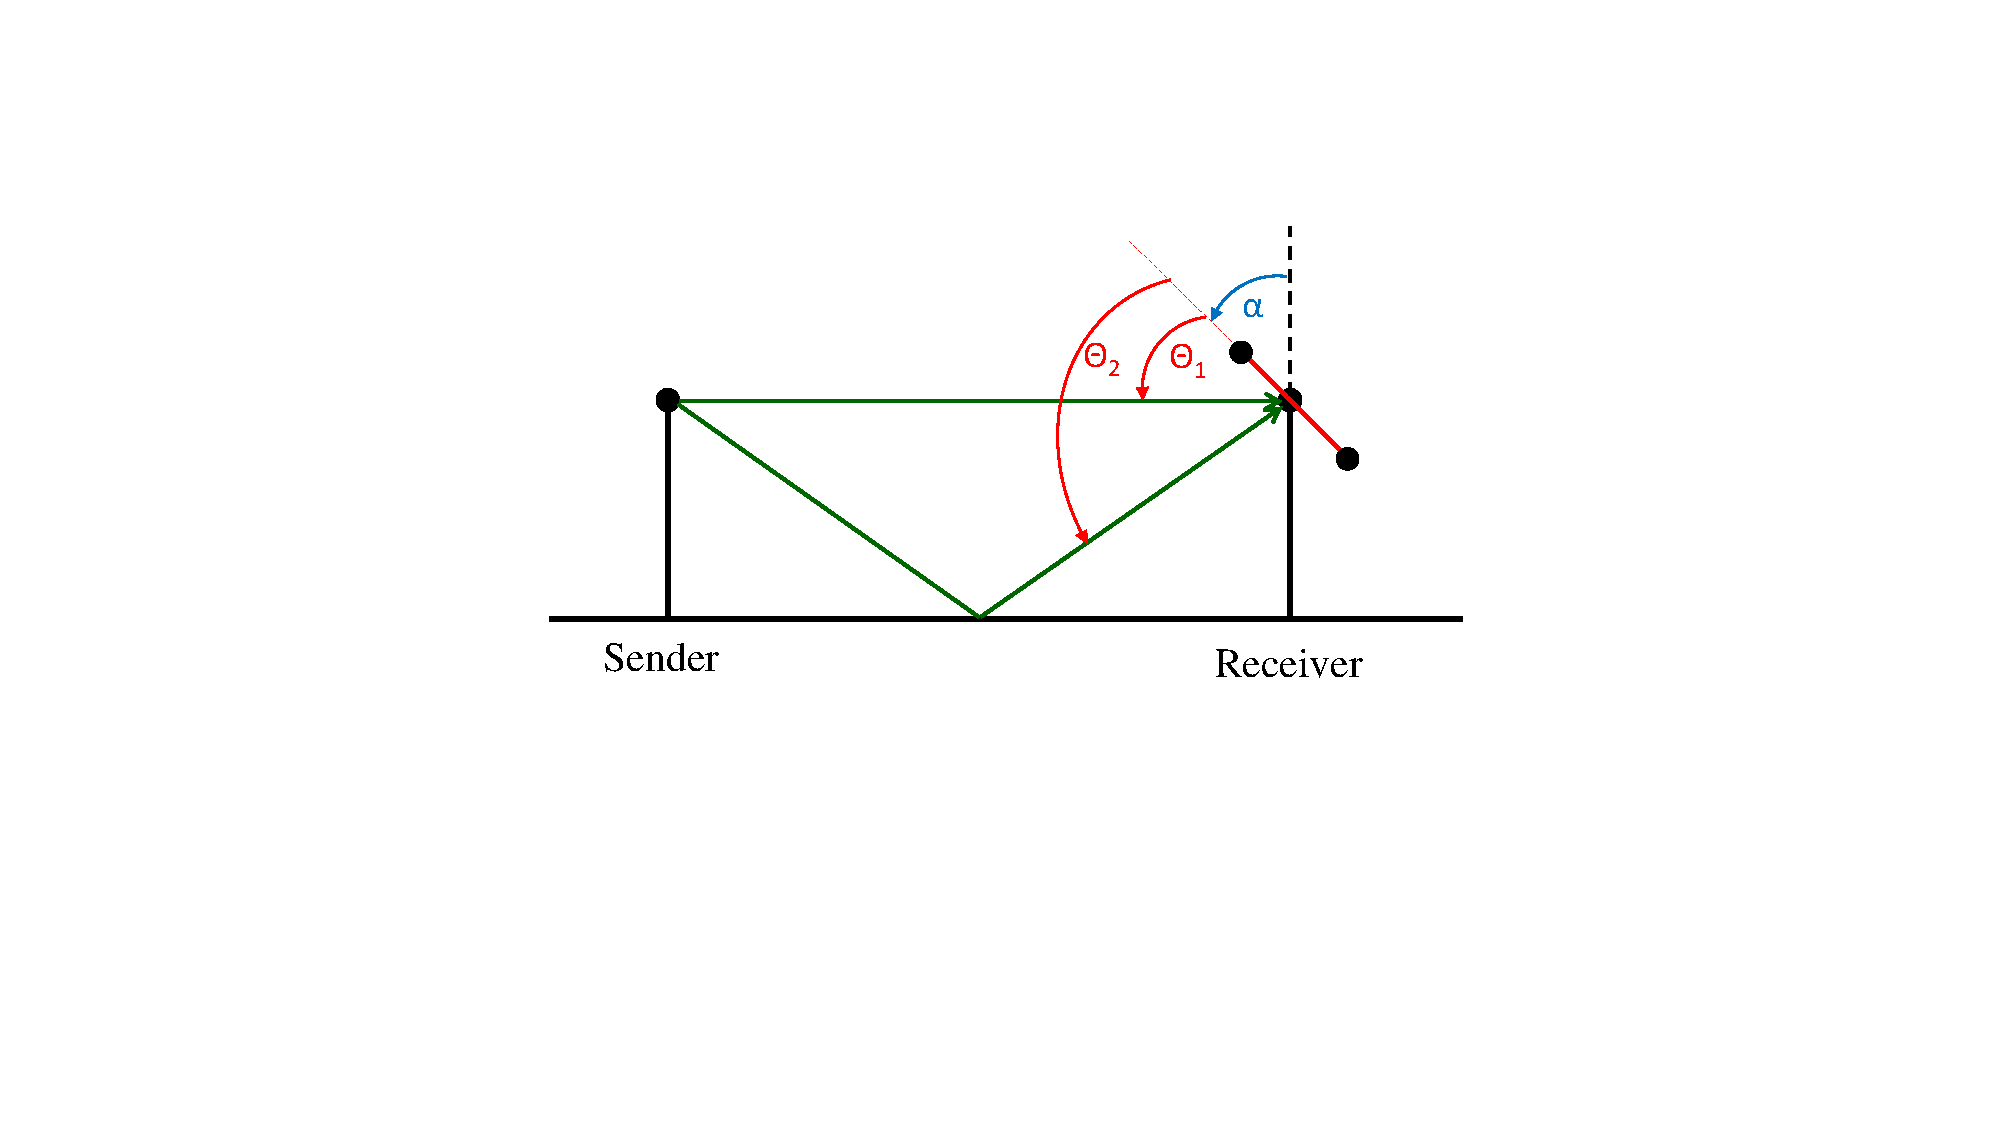
\includegraphics[trim =6cm 7cm 6cm 4cm, clip, width=0.70\textwidth]{graphics/Spatial_filtering_antenna_example_alpha_opt.pdf}
	\caption{Example of a spatial filtering with ULA and tilt angle $\alpha$}
	\label{fig:Spatial_filtering_antenna_example_alpha_opt}
\end{figure}
Choose $\alpha_{opt}$ such that $\vec{a}^H(\Theta_1)\vec{a}(\Theta_2)=0$ (see figure \ref{fig:Spatial_filtering_antenna_example_alpha_opt}).\\
$\ma{A}^H\ma{A}=\mat{\vec{a}^H(\Theta_1)\\\vec{a}^H(\Theta_2)}\mat{\vec{a}(\Theta_1)&\vec{a}(\Theta_2)}=\mat{M&0\\0&M}=M\ma{I}$\\ \\

\textbf{Example:}\\
M=2 \pfeil 2 antennas\\
\begin{figure}[H]
	\centering
		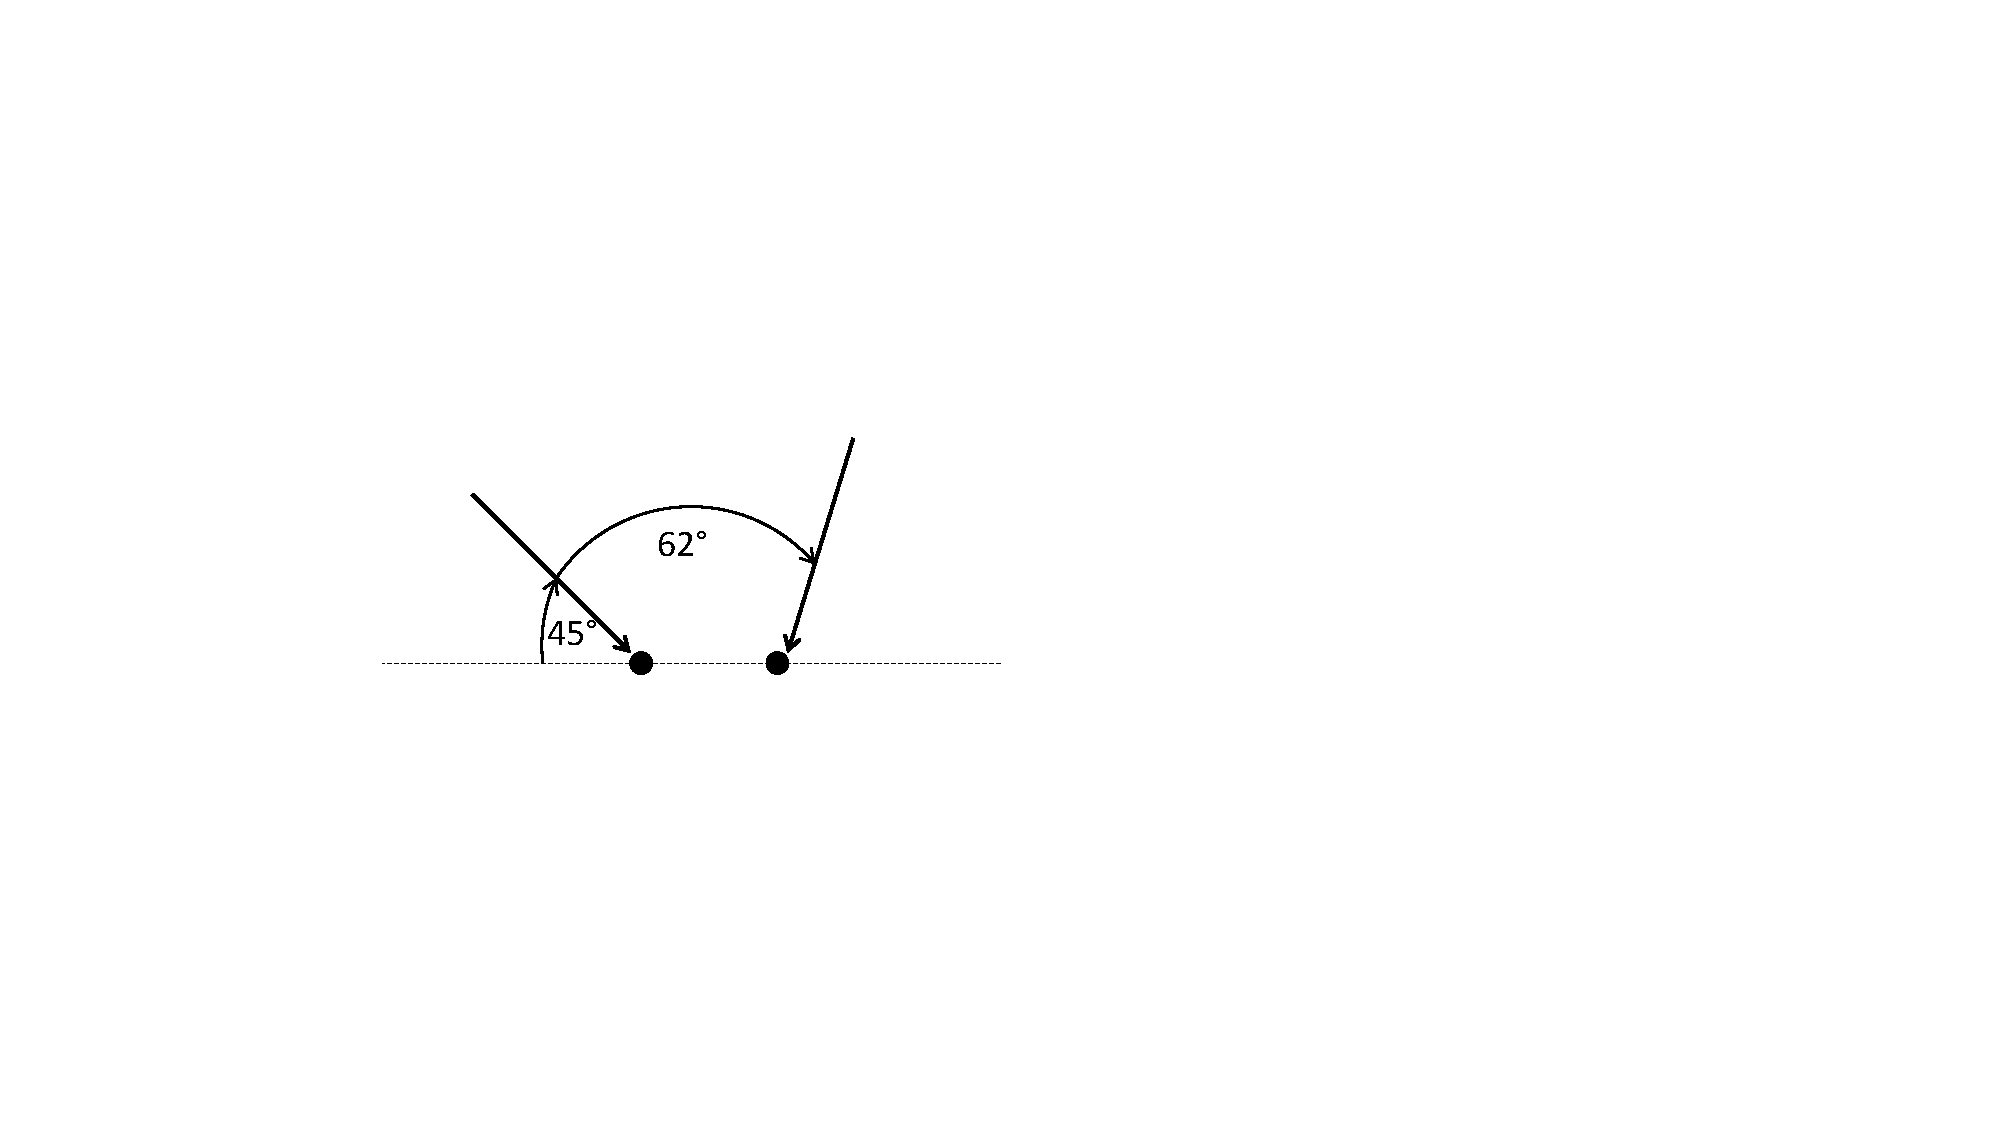
\includegraphics[trim =6cm 7.5cm 14cm 4cm, clip, width=0.50\textwidth]{graphics/LS_filter_example_two_antenna.pdf}
	\caption{Example for $M=2$ and different angles of the arriving signals}
	\label{fig:LS_filter_example_two_antenna}
\end{figure}
$\vec{a}^H(\Theta_1)\vec{a}(\Theta_2)=0$
\end{doublespace}

\subsection{Case 2: Improved Least-Squares - BLUE}
\begin{doublespace}
$\rightarrow$ \textbf{B}est \textbf{L}inear \textbf{U}nbiased \textbf{E}stimator (BLUE)\\
$\ma{X}=\ma{A}\ma{S}+\ma{\nu}$\\
$\ma{W}^H\ma{X}=\underbrace{\ma{W}^H\ma{A}}_{\ma{I}\text{ (unbiased)}}\ma{S}+\underbrace{\ma{W}^H\ma{\nu}}_{\text{Estimation Noise}}$\\
$\ma{W}_{BLUE}=\arg\min\limits_{\ma{W}} E[||\ma{W}^H\ma{\nu}||_F^2],\quad \text{s. t.} \ma{W}^H\ma{A}=\ma{I}_d$\\
\begin{flalign*}
E[||\ma{W}^H\ma{\nu}^H||_F^2]&=E[\trace(\ma{W}^H\ma{\nu}\ma{\nu}^H\ma{W})]
=\trace E[\ma{W}^H\ma{\nu}\ma{\nu}^H\ma{W}]
=\trace(\ma{W}^H \overbrace{E[\ma{\nu}\ma{\nu}^H]}^{N\cdot \ma{R}_\nu}\ma{W})&&\\
&=N\cdot \trace(\ma{W}^H\ma{R}_\nu\ma{W})
\end{flalign*}
$\ma{W}=\mat{\vec{w}_1&\vec{w}_2&\shdots&\vec{w}_d}$\\
$\ma{W}^H\ma{A}=\ma{I}_d \Leftrightarrow\quad \vec{w}_1^H\ma{A}=\vec{e}_1^T,\quad\vec{w}_2^H\ma{A}=\vec{e}_2^T,\quad\ldots,\quad\vec{w}_d^H\ma{A}=\vec{e}_d^T$\\
Lagrange function with equality constraints:\\
$\mathcal{L}=\trace(\ma{W}^H\ma{R}_\nu\ma{W})+2\Re{(\vec{e}_1^T-\vec{w}_1^H\ma{A})\vec{\lambda}_1}+ \ldots + 2\Re{(\vec{e}_d^T-\vec{w}_d^H\ma{A})\vec{\lambda}_d}$\\
$\with \mat{\vec{\lambda}_1 & \vec{\lambda}_2 & \shdots & \vec{\lambda}_d}=:\ma{\lambda}$\\
\begin{flalign*}
\with\trace\left((\ma{I}-\ma{W}^H\ma{A})\ma{\lambda}\right)&=\trace \mat{\vec{e}_1^T-\vec{w}_1^H\ma{A}\\\svdots\\\vec{e}_d^T-\vec{w}_d^H\ma{A}}\mat{\vec{\lambda}_1&\shdots&\vec{\lambda}_d}&&\\
&=(\vec{e}_1^T-\vec{w}_1^H\ma{A})\lambda_1+(\vec{e}_2^T-\vec{w}_2^H\ma{A})\lambda_2+\ldots+(\vec{e}_d^T-\vec{w}_d^H\ma{A})\lambda_d
\end{flalign*}
\begin{flalign*}
\mathcal{L}&=\trace(\ma{W}^H\ma{R}_\nu\ma{W})+2\Re{(\trace(\ma{I}-\ma{W}^H\ma{A})\ma{\lambda}}&&\\
&=\trace(\ma{W}^H\ma{R}_\nu\ma{W})+\trace((\ma{I}-\ma{W}^H\ma{A})\ma{\lambda})+\trace(\ma{\lambda}^H(\ma{I}-\ma{A}^H\ma{W})
\end{flalign*}
$\frac{\partial\mathcal{L}}{\partial\ma{W}^*}=\ma{R}_\nu\ma{W}-\ma{A}\ma{\lambda}\stackrel{!}{=}0 \Rightarrow \ma{W}=\ma{R}_\nu^{-1}\ma{A}\ma{\lambda},\quad \ma{W}^H=\ma{\lambda}^H\ma{A}^H\ma{R}_\nu^{-1}$\\
$\ma{W}^H\ma{A}=\ma{I}=\ma{\lambda}^H\ma{A}^H\ma{R}_\nu^{-1}\ma{A}=\ma{I}$\\
$\ma{\lambda}^H=(\ma{A}^H\ma{R}_\nu^{-1}\ma{A})^{-1}$\\
\mybox{
$\ma{W}_{BLUE}^H=(\ma{A}^H\ma{R}_\nu^{-1}\ma{A})^{-1}\ma{A}^H\ma{R}_\nu^{-1}$
}\\

$\ma{R}_\nu=\const\cdot\ma{I} \Rightarrow \ma{W}_{BLUE}=\ma{W}_{LS}$\pfeil white noise\\
Reconstruction of the signal:\\
$\ma{\hat{S}}=\ma{S}+\ma{W}_{BLUE}^H\ma{\nu}$\\
Calculate SNR:\\
$E[||\ma{W}_{BLUE}^H\ma{\nu}||_F^2]=\trace E[\ma{W}_{BLUE}\ma{\nu}\ma{\nu}^H\ma{W}_{BLUE}]=N\trace (\ma{W}_{BLUE}^H\ma{R}_\nu\ma{W}_{BLUE})$\\
$SNR_{BLUE}=\frac{\trace \ma{R}_s}{\trace (\ma{W}_{BLUE}^H\ma{R}_\nu\ma{W}_{BLUE})}$\\
With: $\ma{W}_{BLUE}^H\ma{R}_\nu\ma{W}_{BLUE}=\underbrace{\underbrace{(\ma{A}^H\ma{R}_\nu^{-1}\ma{A})^{-1}\ma{A}^H\ma{R}_\nu^{-1}}_{\ma{W}_{BLUE}}\underbrace{\ma{R}_\nu\ma{R}_\nu^{-1}}_{\ma{I}}\ma{A}}_{\ma{I}}(\ma{A}^H\ma{R}_\nu^{-1}\ma{A})$\\
\mybox{
$SNR_{BLUE}=\frac{\trace \ma{R}_s}{\trace((\ma{A}^H\ma{R}_\nu^{-1}\ma{A})^{-1})}$\\
}
\mybox{
$SNR_{LS}=\frac{\trace \ma{R}_s}{\trace(\ma{A}^+\ma{R}_\nu(\ma{A}^+)^H)};\qquad \ma{A}^+=(\ma{A}^H\ma{A})^{-1}\ma{A}^H$
}\\ \\
BLUE and LS method are identical if:\\
$\ma{R}_\nu=\const\cdot\ma{I}\quad$ or $\quad M=d \Leftrightarrow SNR_{LS}=SNR_{BLUE}$\\
\Ra\ Only improvement for:
\begin{itemize}
	\item More sensors ($d<M$)
	\item $\ma{R}_\nu\neq\const\cdot\ma{I}$ (no white noise, but colored noise)
\end{itemize}

\subsubsection{Introduction signal correlation matrix as a substitution of the noise correlation matrix}
$\ma{W}_{BLUE}^H =(\ma{A}^H\ma{R}_\nu^{-1}\ma{A})^{-1}\ma{A}^H\ma{R}_\nu^{-1}$\\
\Ra\ We need to know \ma{A} and $\ma{R}_\nu$ or just \ma{A} and allow \emph{latency time}.\\ \\
\textbf{Why can we trade in $\ma{R}_\nu$ for latency time?}\\
$\ma{W}_{BLUE}^H =(\ma{A}^H\ma{R}_x^{-1}\ma{A})^{-1}\ma{A}^H\ma{R}_x^{-1}$\qquad
where $\ma{R}_x=E[\vec{x}[n]\vec{x}^H[n]]$ is the signal correlation matrix\\
The orginal optimization is:\\
$\ma{W}_{BLUE}=\arg\min E[||\ma{W}^H\ma{\nu}||_F^2],\quad \text{s. t. } \ma{W}^H\ma{A}=\ma{I}$\\
Now substitude Noise $\ma{\nu}$ with $\ma{X}$:\\
$\ma{X}=\ma{A}\ma{S}+\ma{\nu}\pfeil$with optimal $\ma{W}^H$ \pfeil $\qquad \ma{W}^H\ma{X}\left.\right|_{\ma{W}^H\ma{A}=\ma{I}}=\ma{S}+\ma{W}^H\ma{\nu}$\\
substitutional optimization:
\begin{flalign*}
E[\ma{W}^H\ma{X}\ma{X}^H\ma{W}]\left.\right|_{\ma{W}^H\ma{A}=\ma{I}}&=E\left[(\ma{S}+\ma{W}^H\ma{\nu})(\ma{S}^H+\ma{\nu}^H\ma{W})\right]&&\\
&\underbrace{=}_{E[\ma{S}\ma{\nu}]=0} E[\ma{S}^H\ma{S}]+\ma{W}^H\ma{R}_\nu\ma{W}
\end{flalign*}
Note: $E[\ma{S}\ma{\nu}]=0$ means that noise and signal are uncorrelated, which can be assumed usually.\\

$\underbrace{\trace{E[\ma{W}^H\ma{X}\ma{X}^H\ma{W}]}}_{E[||\ma{W}^H\ma{X}||_F^2}\left.\right|_{\ma{W}^H\ma{A}=\ma{I}}=\trace(E[\ma{S}\ma{S}^H])+\underbrace{\trace(\ma{W}^H\ma{R}_\nu\ma{W})}_{E[||\ma{W}^H\ma{\nu}||_F^2}$\\
If $\ma{W}\ma{A}=\ma{I}$ is met, then $\min||\ma{W}^H\ma{X}||_F^2$ will minimize $E[||\ma{W}^H\ma{\nu}|_F^2]$ because $\ma{W}^H\ma{X}=\ma{S}\ma{W}^H\ma{\nu}$. $\tr (E[\ma{S}\ma{S}^H]) = \const$\\
So we can exchange $\ma{R}_\nu$ with $\ma{R}_x$.\\
Estimate $\ma{R}_x$ as:
\begin{flalign*}
\ma{\hat{R}}_x=\frac{1}{N}\sum\limits_{k=0}^{N-1}\vec{x}[n+k]\vec{x}^H[n+k]=\frac{1}{N} \ma{X}\ma{X}^H
\end{flalign*}
There is no need to know the noise, but we need to know N snapshots to fill $\ma{X}$. \\\pfeil therefore latency time! \\
\mybox{
$\ma{\hat{W}}_{BLUE}^H=\left(\ma{A}^H\left(\ma{X}\ma{X}^H\right)^{-1}\ma{A}\right)^{-1}\ma{A}^H\left(\ma{X}\ma{X}^H\right)^{-1}$\\
Note: $\ma{\hat{W}}_{BLUE}^H$ needs to be computed before we can use the filter. This causes \emph{latency}.\\
$\ma{\hat{S}}_{BLUE}=\ma{\hat{W}}_{BLUE}^H\ma{X} \rightarrow$ Latency!
}
\mybox{
$\ma{W}_{LS}^H=(\ma{A}^H\ma{A})$\\
$\ma{\hat{S}}_{LS}=\ma{W}_{LS}^H\ma{X} \rightarrow$ No latency!\\
}
\end{doublespace}

\subsection{Case 3: LMMSE-Estimator (Linear Minimum Mean Square Error)}
\begin{doublespace}
$\ma{W}_{LMMSE}=\arg\min\limits_{\ma{W}}\underbrace{E[||\ma{\hat{S}}-\ma{S}||_F^2]}_{J}$\\
$\ma{\hat{S}}=\ma{W}^H\ma{X}$\qquad Estimate Signal Matrix\\

Cost Function:
\begin{flalign*}
J&=E[||\ma{W}^H\ma{X}-\ma{S}||_F^2]&&\\
&=E\left[\trace\left((\ma{W}^H\ma{X}-\ma{S})(\ma{X}^H \ma{W} - \ma{S})\right)\right]&&\\
&=\trace\left(\ma{W}^H E[\ma{X}\ma{X}^H]\ma{W}\right) - \trace\left(\ma{W} E[\ma{X}\ma{S}^H]\right) - \trace\left(E[\ma{S}\ma{X}^H]\ma{W}\right) + \trace\left(E\ma{S}\ma{S}^H]\right)
\end{flalign*}
Singal Correlation Matrix: \\ $E[\ma{X}\ma{X}^H]=N\ma{R}_x$ \\ 
Channel output Correlation Matrix: \\$E[\ma{S}\ma{S}^H]=N\ma{R}_S$\\ 
Correlation between Signal and Channel Output:\\ $E[\ma{X}\ma{S}^H]=E\left[(\ma{A}\ma{S}-\ma{\nu})\ma{S}^H\right] = \ma{A}E[\ma{S}\ma{S}^H]+E[\ma{\nu}\ma{S}^H]$ \\ 

With assumimg, that noise and signal are uncorrelated ($E[\ma{\nu}\ma{S}^H]=\ma{0}$) we get:\\
$E[\ma{X}\ma{S}^H] = \ma{A}E[\ma{S}\ma{S}^H] = \ma{A}\ma{R}_s N$\\
With the property $\ma{R}_s=\ma{R}_s^H$ (Recall: All correlation matrices are hermitian matrices) we get for our cost function J:\\
$J=N\trace\left(\ma{W}^H\ma{R}_x\ma{W}\right)-N\trace\left(\ma{W}^H\ma{A}\ma{R}_s\right) - N \trace\left(\ma{R}_s\ma{A}^H\ma{W}\right) + N\trace\left(\ma{R}_s\right)$\\ \\
Now what is our filter matrice $\ma{W}_{LMMSE}$?\\
$\frac{\partial J}{\partial \ma{W}^*}=N\ma{R}_x\ma{W}-N\ma{A}\ma{R}_s\stackrel{!}{=}0$\\
\mybox{
$\ma{W}_{LMMSE}=\ma{R}_x^{-1}\ma{A}\ma{R}_s$ 
\qquad or\qquad
$\ma{W}_{LMMSE}^H=\ma{R}_s\ma{A}^H\ma{R}_x^{-1}$
}
\textbf{Derive Correlation Matrices}
\begin{flalign*}
\ma{R}_x&=E[\vec{x}[n]\vec{x}^H[n]]\underbrace{=}_{\text{stationarity}}\frac{1}{N}\sum\limits_{k=0}^{N-1}E[x[n+k]x^h[n+k]]&&\\
&=\frac{1}{N}E[\ma{X}\ma{X}^H]&&\\
&=\frac{1}{N}E\left[(\ma{A}\ma{S}+\ma{\nu})(\ma{A}^H\ma{A}^H+\ma{\nu}^H)\right]; \qquad \ma{X}=\ma{A}\ma{S}+\ma{\nu}&&\\
&=\frac{1}{N}\left(\ma{A}\underbrace{E[\ma{S}\ma{S}^H]}_{N\ma{R}_s}+\ma{A}\underbrace{E[\ma{S}\ma{\nu}^H]}_{\ma{0}}+\underbrace{E[\ma{\nu}\ma{S}^H]}_{\ma{0}}\ma{A}^H+\underbrace{E[\ma{\nu}\ma{\nu}^H]}_{N\ma{R}_\nu}\right)
\end{flalign*}
\mybox{
$\ma{R}_x=\ma{A}\ma{R}_s\ma{A}^H+\ma{R}_\nu$
}
\\ \\
Assueme: \ma{A} has got full column rank \Ra $\ma{A}^+\ma{A}=\ma{I}$ therefore we can obtain $\ma{R}_S$\\
\mybox{
$\ma{R}_s=\ma{A}^+(\ma{R}_x-\ma{R}_\nu)(\ma{A}^+)^H$ \pfeil it's not neccessary to know $\ma{R}_S$
}
\mybox{
\begin{flalign*}
\ma{W}_{LMMSE}^H&=\ma{A}^+(\ma{R}_x-\ma{R}_\nu)(\ma{A}^+)^H\ma{R}_x^{-1}&&\\
&=(\ma{A}^H\ma{A})^{-1}\ma{A}^H(\ma{R}_x-\ma{R}_\nu)\ma{A}(\ma{A}^H\ma{A})^{-1}\ma{R}_x^{-1}
\end{flalign*}
}
$\ma{\hat{R}}_x=\frac{1}{N}\ma{X}\ma{X}^H \qquad \ma{R}_\nu=\ma{R}_x\left.\right|_{\ma{S}=\ma{0}};$\\
$ \ma{R}_x^{-1}$ has to be regular (squares matrix with det $\neq 0)\pfeil N\geq M$\\
Where $M$ is the number of sensors and $N$ the number of snapshots we take.\\
$\ma{R}_\nu=\frac{1}{N}\ma{X}\ma{X}^H \left.\right|_{\ma{S}=\ma{0}}$

\Ra Possibility: Run BLUE, LS and LMMSE in parallel and choose the one that performes best. Decide on the parameter checksum / error routine which has the least error. 
\end{doublespace}

\newpage
\section{Estimate the Steering Matrix}
Estimation of $\ma{A}$ without knowledge of $\ma{S}$:\\
$\ma{X}=\ma{A}\ma{S}+\ma{\nu}$\\
To determine \ma{A} we could use pilots like we did already earlier in this lecture. But here we want to derive a method that works without sending known symbols over the channel. This is called "Blind Channel Estimation".\\ \\
\underline{Non-linear estimation for \ma{A}:}\\
\begin{doublespace}
$\ma{A}=\mat{\vec{a}[\Theta_1]&\vec{a}[\Theta_2]&\shdots&\vec{a}[\Theta_d]} \in\mathbb{C}^{M\times d}$\\
\begin{figure}[H]
	\centering
		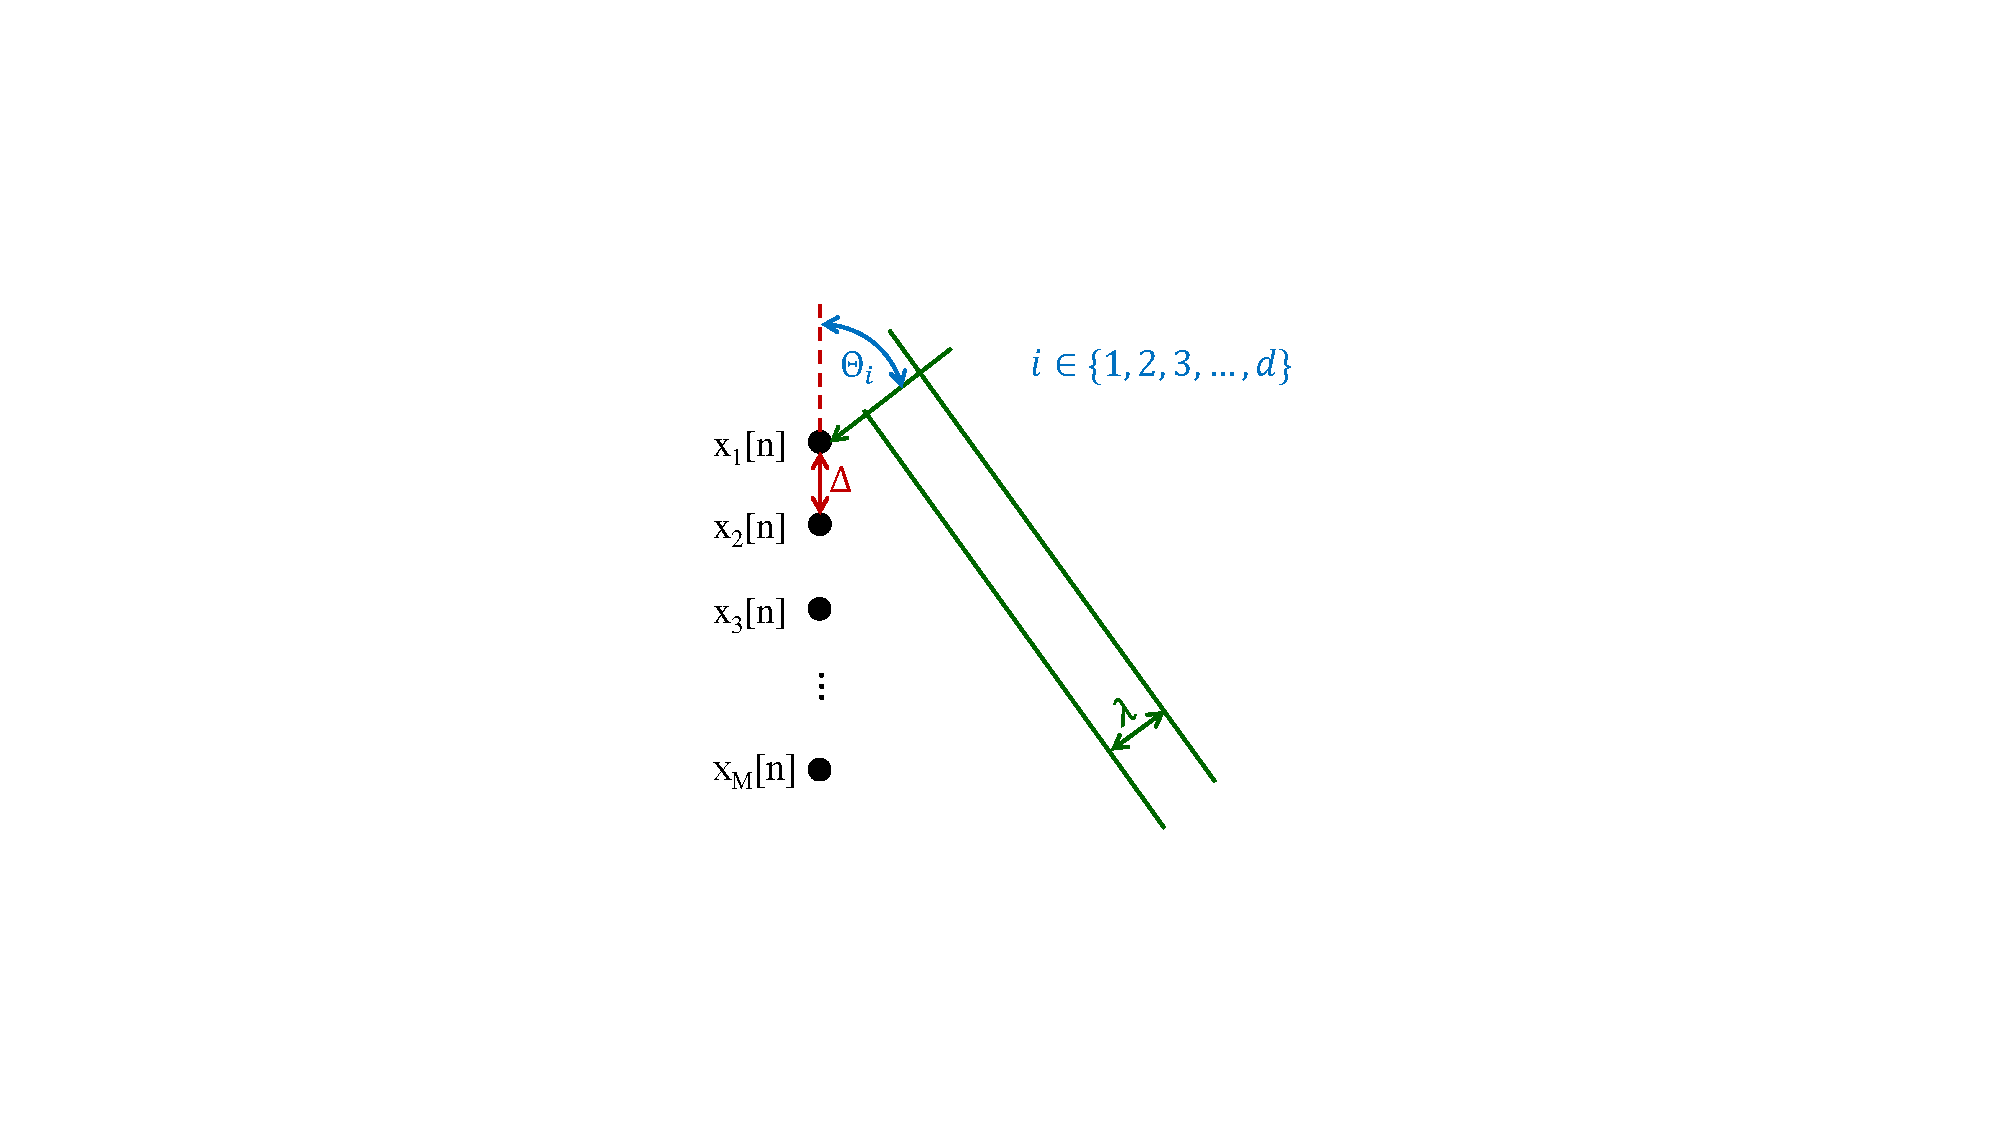
\includegraphics[trim =6cm 5.5cm 6cm 4cm, clip, width=0.70\textwidth]{graphics/ULA_Angle_theta_M_Sensors.pdf}
	\caption{Unform Linear Array (ULA) with $M$ sensors}
	\label{fig:ULA_Angle_theta_M_Sensors}
\end{figure}

$\vec{a}(\Theta_i)=\mat{1\\e^{-\j2\pi\frac{\Delta}{\lambda}\cos(\Theta_i)}\\e^{-2\j2\pi\frac{\Delta}{\lambda}\cos(\Theta_i)}\\e^{-3\j2\pi\frac{\Delta}{\lambda}\cos(\Theta_i)}\\\shdots\\e^{-(M-1)\j2\pi\frac{\Delta}{\lambda}\cos(\Theta_i)}}  $ \\ \\
\mybox{
$\mu:=2\pi\frac{\Delta}{\lambda}\cos(\Theta)\qquad \mu_i:=2\pi\frac{\Delta}{\lambda}\cos(\Theta_i)$\qquad $\mu$ is the phase of the signal.
}\\ \\
$\vec{a}(\mu_i)=\mat{1\\e^{-\j\mu_i}\\e^{-2\j\mu_i}\\e^{-3\j\mu_i}\\\svdots\\\\e^{-(M-1)\j\mu_i}}=\mat{1\\\xi^1\\\xi^2\\\xi^3\\\svdots\\\xi^{M-1}}$ "Vandermonde vector"\\ \\
$\Theta=\arccos\left(\frac{\mu}{2\pi\frac{\Delta}{\lambda}}\right)$\\
$\vec{a}(\mu)=\vec{a}(\mu+2\pi n); \quad n\in\{0,\pm1,\pm2,\ldots\}$\\
\mybox{
What is now the corresponding angle? $\Theta$ or $\Theta'$?\\
$\mu+2\pi n = 2\pi\frac{\Delta}{\lambda}\cos(\Theta')$\\
$\mu=2\pi\frac{\Delta}{\lambda}\cos(\Theta)$
}\\
$2\pi\frac{\Delta}{\lambda}\cos(\Theta)+2\pi n = 2\pi\frac{\Delta}{\lambda}\cos(\Theta')$\\
$\cos(\Theta)+\frac{2\pi n}{2\pi\frac{\Delta}{\lambda}}=\cos(\Theta')$\\
$\Theta'=\arccos\underbrace{\left(\frac{n}{\frac{\Delta}{\lambda}}+\cos(\Theta)\right)}_{\Phi};\quad n\in\{0,\pm1,\pm2,\ldots\}$\\
if $\frac{\Delta}{\lambda} < \frac{1}{2}$ \Ra $n=0$ only possible for existing values $\Theta=\Theta'$\\ \\
if $\frac{\Delta}{\lambda}=\frac{1}{2} \Ra (\Theta,\Theta')\in\{(0,\pi),(\pi,0)\}$\\
Determine the error of $\Theta$ with respect to $\mu$:\\
$\Theta=\arccos\left(\frac{\mu}{2\pi\frac{\Delta}{\lambda}}\right)$\\
$\frac{\partial \Theta}{\partial \mu}=\frac{1}{\Delta/\lambda}\cdot \frac{1}{\sqrt{4\pi^2-\left(\frac{\mu}{\Delta/\lambda}\right)^2}}$\\
$\min\limits_\mu\frac{\partial \Theta}{\partial \mu}=\frac{\partial \Theta}{\partial \mu}\left.\right|_{\mu=0}=\frac{1}{2\pi \frac{\Delta}{\lambda}}$\\
Estimate $\mu$ with error $e_{\mu}=\pm\Delta\mu$\\
Then $\Theta$ with error $e_{\Theta}\approx\frac{\partial \Theta}{\partial \mu}\Delta\mu=\frac{1}{\Delta/\lambda}\cdot \frac{1}{\sqrt{4\pi^2-\left(\frac{\mu}{\Delta/\lambda}\right)^2}}\Delta\mu$\\
Note that the function for $\frac{\partial \Theta}{\partial \mu}$ has a pole:\\
$4\pi^2=\frac{\mu^2}{(\frac{\Delta}{\lambda})^2}; \qquad 4\pi^2(\frac{\Delta}{\lambda})^2=\mu^2 \Rightarrow \mu=2\pi \frac{\Delta}{\lambda}$\\
$\frac{\partial \Theta}{\partial \mu}\left.\right|_{\mu=2\pi \frac{\Delta}{\lambda}} = \infty$\\
if $\frac{\Delta}{\lambda} = \frac{1}{2} \Rightarrow \mu=\pi$ is worst for estimating $\Theta$
\Ra in practice we can therefore allow $\frac{\Delta}{\lambda}=\frac{1}{2}$ because the situition is anyway very bad for estimating $\Theta$.\\ \\
$\frac{\partial \Theta}{\partial \mu} \leq 2 \min \frac{\partial \Theta}{\partial \mu}$\\

\begin{figure}[H]
	\centering
		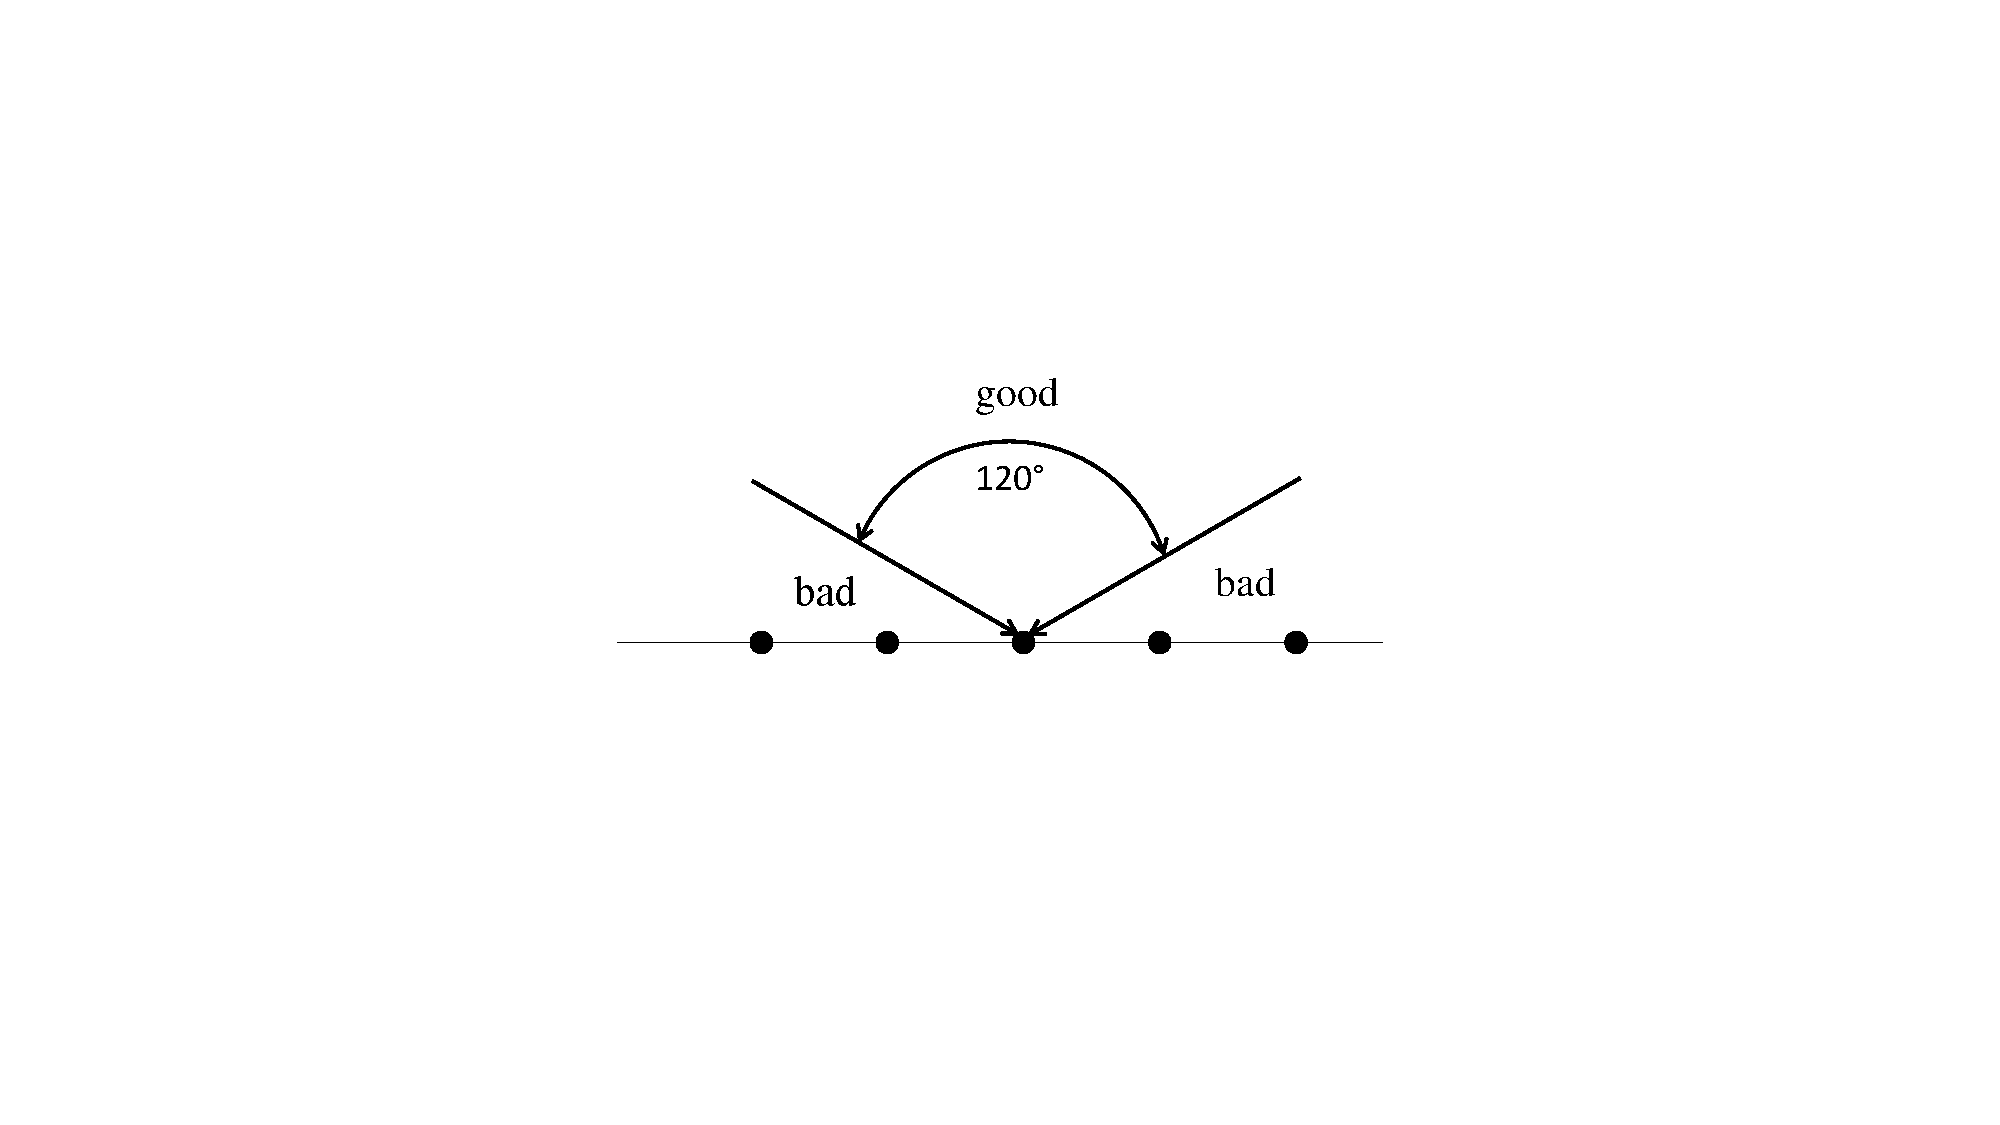
\includegraphics[trim =8cm 8cm 8cm 6cm, clip, width=0.70\textwidth]{graphics/Behaviour_of_estimation_of_mu_for_regions.pdf}
	\caption{Behaviour of the estimated $\mu$ for different angles }
	\label{fig:Behaviour_of_estimation_of_mu_for_regions}
\end{figure}

\begin{tabular}{rl}
d: & Number of arriving wavefronts\\
 & unknown to the receiver\\
 & needs to be estimated\\
$\Theta_1,\,\Theta_2,\ldots\Theta_d$:& Directions of arrival (DoA)\\
\end{tabular}\\
$\mu_i=2\pi \frac{\Delta}{\lambda}\cos(\Theta_i)$\\
\textbf{From now on we choose} $\frac{\Delta}{\lambda}=\frac{1}{2}$\\
Then:\\
\mybox{
$\mu_i=\pi\cos(\Theta_i)$
}
\begin{figure}[H]
	\centering
		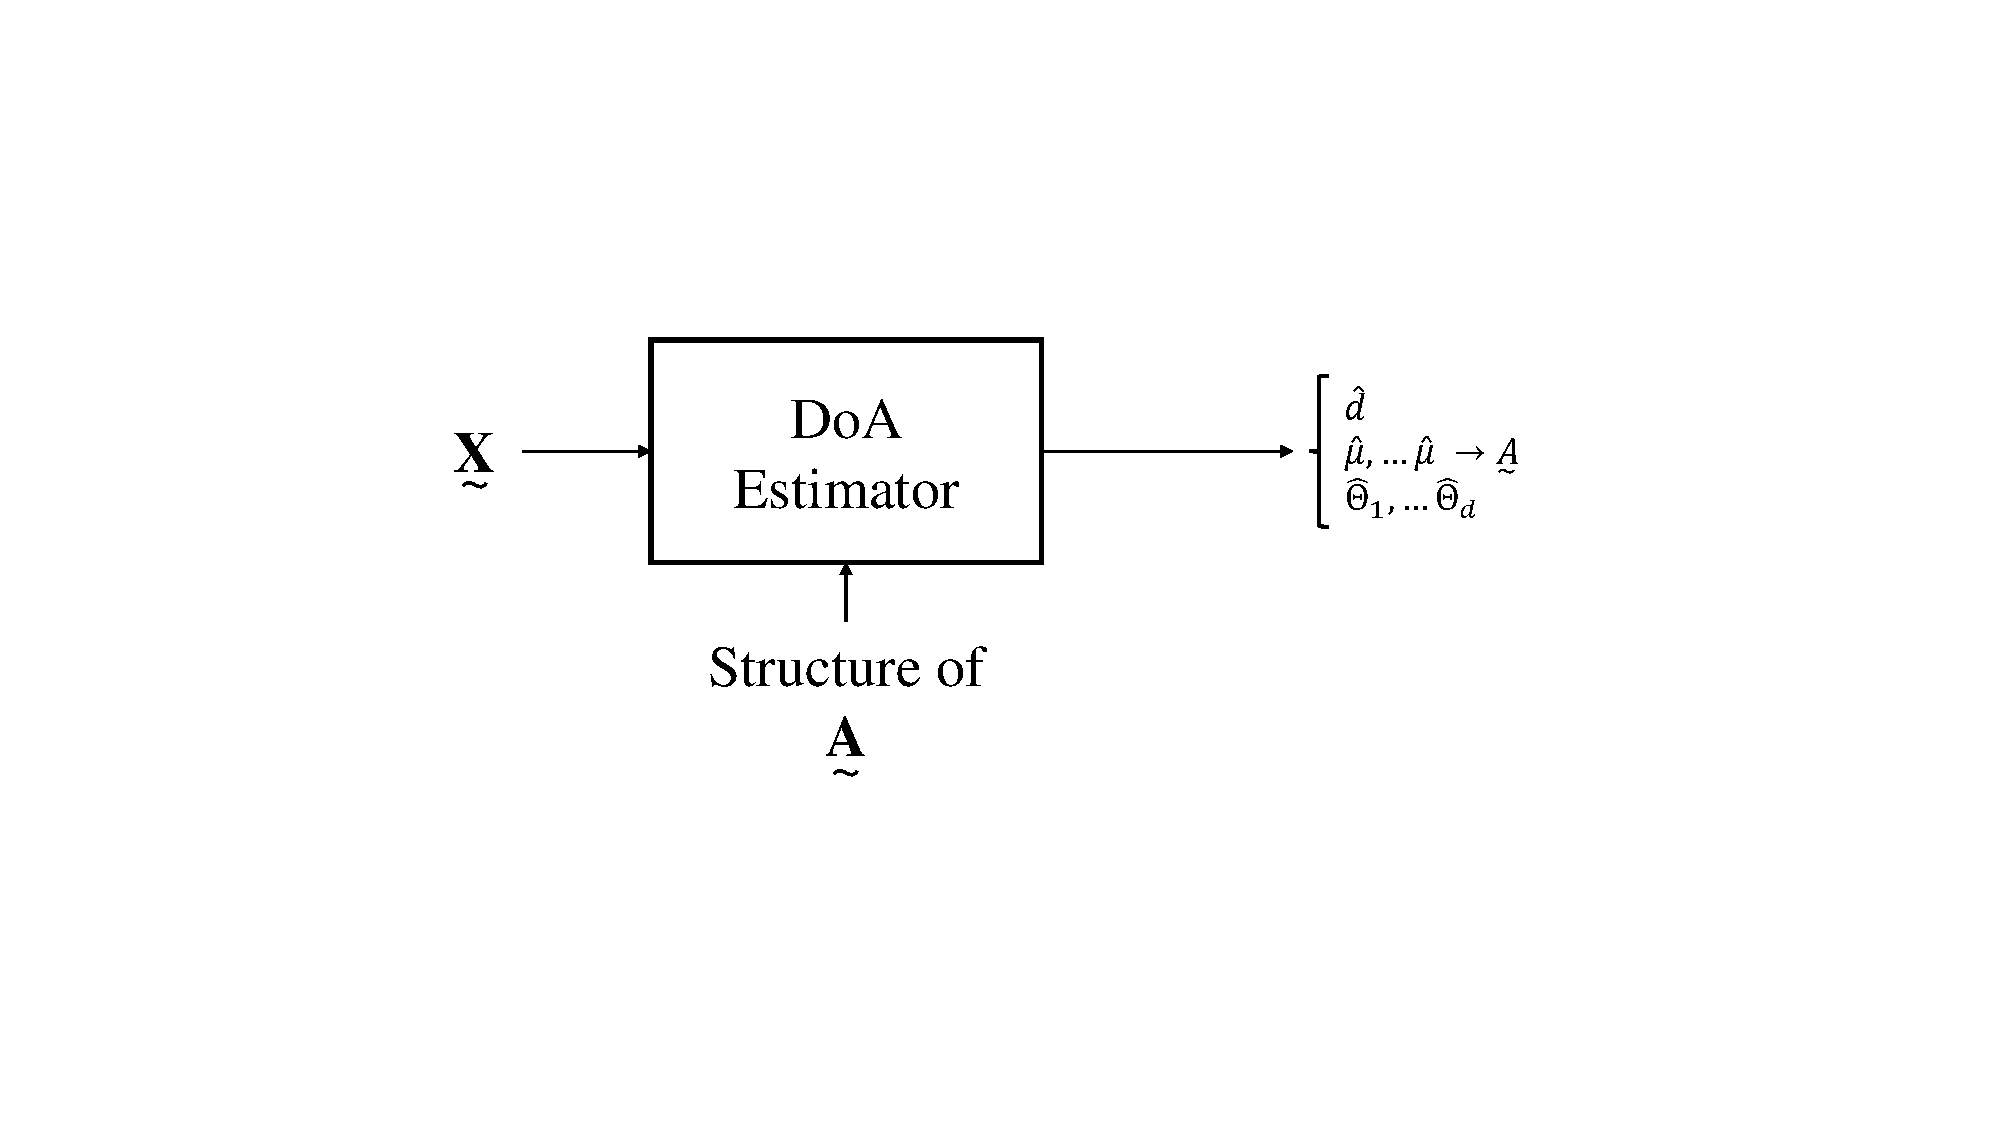
\includegraphics[trim =4cm 5.5cm 4cm 4cm, clip,width=0.70\textwidth]{graphics/Block_diagram_DoA_estimator.pdf}
	\caption{Simple block diagram of a DoA (Dimension of Arrival) Estimator}
	\label{fig:Block_diagram_DoA_estimator}
\end{figure}
\end{doublespace}

\subsection{Space-Discrete Fourier Transform}
\begin{figure}[H]
	\centering
		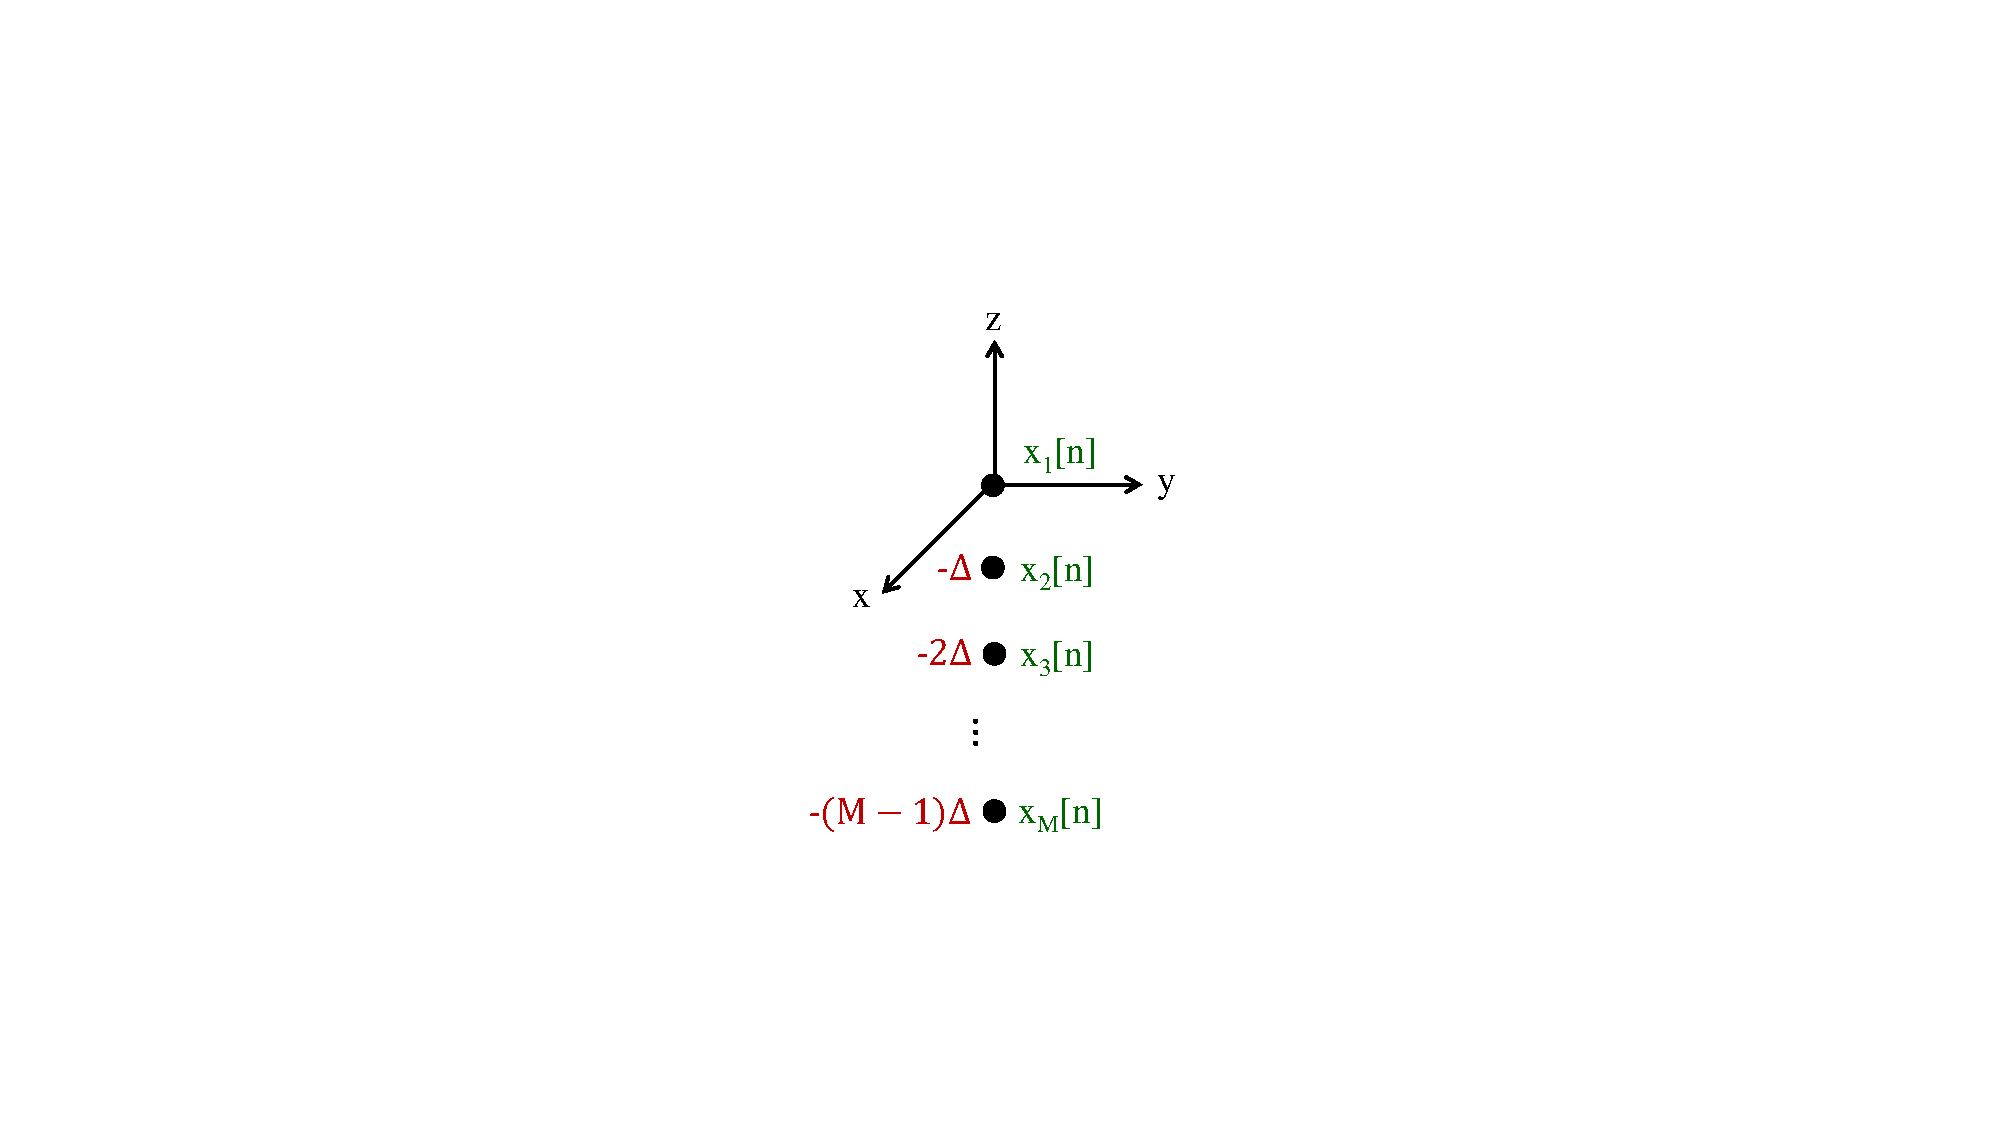
\includegraphics[trim =6cm 4.5cm 6cm 4cm, clip, width=0.70\textwidth]{graphics/ULA_space-discrete_fourier_transform.pdf}
	\caption{Sensor arrangement for the Space-Discrete Fourier Transform}
	\label{fig:ULA_space-discrete_fourier_transform}
\end{figure}


\begin{itemize}
	\item sampling in space: $x_k[n]=g(z)\left.\right|_{z=-(k-1)\Delta}$ \pfeil $g(z)= field$
	\item Space Fourier Transform: $G(\tilde{f})=\int\limits_{-\infty}^{\infty}{g(z)e^{-\j2\pi\tilde{f}z}dz}$
\end{itemize}
The "Space Fourier Transform" is related to the Time Fourier Transform, just replace time by space ($t$ by $z$) and the frequency $f$ by the space frequency $\tilde{f}$.\\
$\tilde{f}$: space-frequency $\qquad [\tilde{f}]=\frac{1}{m}=m^{-1}$\\
\Ra Problem: g(z) is not known to us everywhere. We just know it at some discrete points. Therefor we sample it:\\
$h(z)=g(z)\sum\limits_{k=0}^{M-1}{\delta(z+\Delta k)}$\\
\rule{\textwidth}{0.4pt}
\textbf{Recall:}\\
$\delta(z)=0, \forall z \neq 0$\\
$\int\limits_{-\infty}^{\infty}{\delta(z)dz}=1$\\
\rule{\textwidth}{0.4pt}
\begin{flalign*}
H(\tilde{f})&=\int\limits_{-\infty}^{\infty}{h(z)e^{-\j2\pi\tilde{f}z}dz}&&\\
&=\int\limits_{-\infty}^{\infty}{g(z)\left(\sum\limits_{k=0}^{M-1}{\delta(z+\Delta k)}\right)e^{-\j2\pi\tilde{f}z}dz}&&\\
&=\sum\limits_{k=0}^{M-1}{\int\limits_{-\infty}^{\infty}{g(z)\delta(z+\Delta k)e^{-\j2\pi\tilde{f}z}dz}}&&\\
&=\sum\limits_{k=0}^{M-1}{\int\limits_{-\infty}^{\infty}{g(-\Delta k)\delta(z+\Delta k)e^{+\j2\pi\tilde{f}\Delta k}dz}}&&\\
&=\sum\limits_{k=0}^{M-1}{g(-\Delta k)e^{+\j2\pi\tilde{f}\Delta k}}\underbrace{\int\limits_{-\infty}^{\infty}{\delta(z+\Delta k)dz}}_{=1}&&\\
&=\sum\limits_{k=0}^{M-1}{\underbrace{g(-\Delta k)}_{x_{k+1}[n]}e^{+\j2\pi\tilde{f}\Delta k}dz}
\end{flalign*}
For convenience we define $\mu:=2\pi\tilde{f}\Delta$.\\
\mybox{
$H(\tilde{f})=\sum\limits_{k=0}^{M-1}{x_{k+1}[n]e^{\j\mu k}}$
}\\
$\mu$: Normalized space angular frequency (dimensionless)
Compare:\\ $\underbrace{2\pi f }_{\omega}T=\omega T = \Omega$\qquad
$2\pi\tilde{f}\Delta = \mu$ \\ \\
Recall the steering vector $\vec{a}(\mu)$ and the received signal vector $\vec{x}[n]$:\\
$\vec{a}(\mu)=\mat{1\\e^{-\j\mu}\\e^{-2\j\mu}\\e^{-3\j\mu}\\\svdots\\\\e^{-(M-1)\j\mu}}; \qquad \vec{x}[n]=\mat{\\x_2[n]\\x_3[n]\\x_4[n]\\\svdots\\x_M[n]}$\\

\mybox{
$H(\mu)=\vec{a}^H(\mu)\vec{x}[n]$\\
Note: $H(\mu)$ is just an other notation of $H(\tilde{f})$
}

\paragraph{Fourier Periodogram}
\begin{flalign*}
S(\mu):&=\frac{1}{N}\sum\limits_{n=1}^{N}{\left|\vec{a}^H(\mu)\vec{x}[n]\right|^2}=\bar{\abs{H(\mu)}^2}&&\\
&=\frac{1}{N}\sum\limits_{n=1}^{N}{\vec{a}^H(\mu)\vec{x}[n]\vec{x}^H[n]\vec{a}(\mu)}&&\\
&=\vec{a}^H(\mu)\underbrace{\left(\sum\limits_{n=1}^{N}{\vec{x}[n]\vec{x}^H[n]}\right)}_{\ma{\hat{R}}_x=\frac{1}{N}\ma{X}\ma{X}^H}\vec{a}(\mu)
\end{flalign*}
\mybox{
$S(\mu)=\vec{a}^H(\mu)\ma{\hat{R}}_x\vec{a}(\mu)\qquad \mu=2\pi\frac{\Delta}{\lambda}\cos(\Theta)$
}
Search peaks in the periodogram to find $\mu$ of incoming wave fronts.
\\ \ \\
\textbf{Example:}\\
$d=1$ (only one arriving wavefront)\\
no noise, continuous wave $s[n]=\const=1$\\
$\vec{x}[n]=\vec{a}(\mu_1)s[n]=\vec{a}(\mu_1); \qquad \mu_1=2\pi\frac{\Delta}{\lambda}\cos(\Theta_1)$ \quad find: $\Theta_1$\\
$\ma{\hat{R}}_x = \frac{1}{N}\sum\limits_{n=1}^{N}{\vec{a}(\mu_1)\vec{a}^H(\mu_1)} = \vec{a}(\mu_1)\vec{a}^H(\mu_1)$\\
\begin{flalign*}
S(\mu)&=\vec{a}^H(\mu)\ma{\hat{R}}_x\vec{a}(\mu)&&\\
&=\vec{a}^H(\mu)\vec{a}(\mu_1)\vec{a}^H(\mu_1)\vec{a}(\mu)&&\\
&=\left|\vec{a}^H(\mu)\vec{a}(\mu_1)\right|^2&&\\
&=\left|\sum\limits_{k=0}^{M-1}{e^{\j(\mu-\mu_1)k}}\right|^2
\end{flalign*}
\rule{\textwidth}{0.4pt}
\textbf{Recall:}\\
$s=1+q+q^2+\ldots+q^{M-1}$\\
$sq=q+q^2+\ldots+q^{M-1}+q^M$\\
$sq-s=q^M-1 \Rightarrow s=\frac{q^M-1}{q-1}$ (geometric series)\\
$q=e^{\j(\mu-\mu_1)}$\\
\rule{\textwidth}{0.4pt}

\begin{flalign*}
S(\mu)&=\left|\frac{e^{\j(\mu-\mu_1)M}-1}{e^{\j(\mu-\mu_1)}-1}\right|^2&&\\
&=\left|\frac{e^{\j(\mu-\mu_1)\frac{M}{2}}\cdot\left(e^{\j(\mu-\mu_1)\frac{M}{2}}-e^{-\j(\mu-\mu_1)\frac{M}{2}}\right)}{e^{\j\frac{(\mu-\mu_1)}{2}}\cdot\left(e^{\j\frac{(\mu-\mu_1)}{2}}-e^{-\j\frac{(\mu-\mu_1)}{2}}\right)}\right|^2&&\\
&=\left(\frac{\sin\left(\frac{M}{2}(\mu-\mu_1)\right)}{\sin\left(\frac{1}{2}(\mu-\mu_1)\right)}\right)^2
\end{flalign*}
$\lim\limits_{\mu\rightarrow\mu_1}S(\mu)=M^2$\\

\begin{figure}[H]
	\centering
		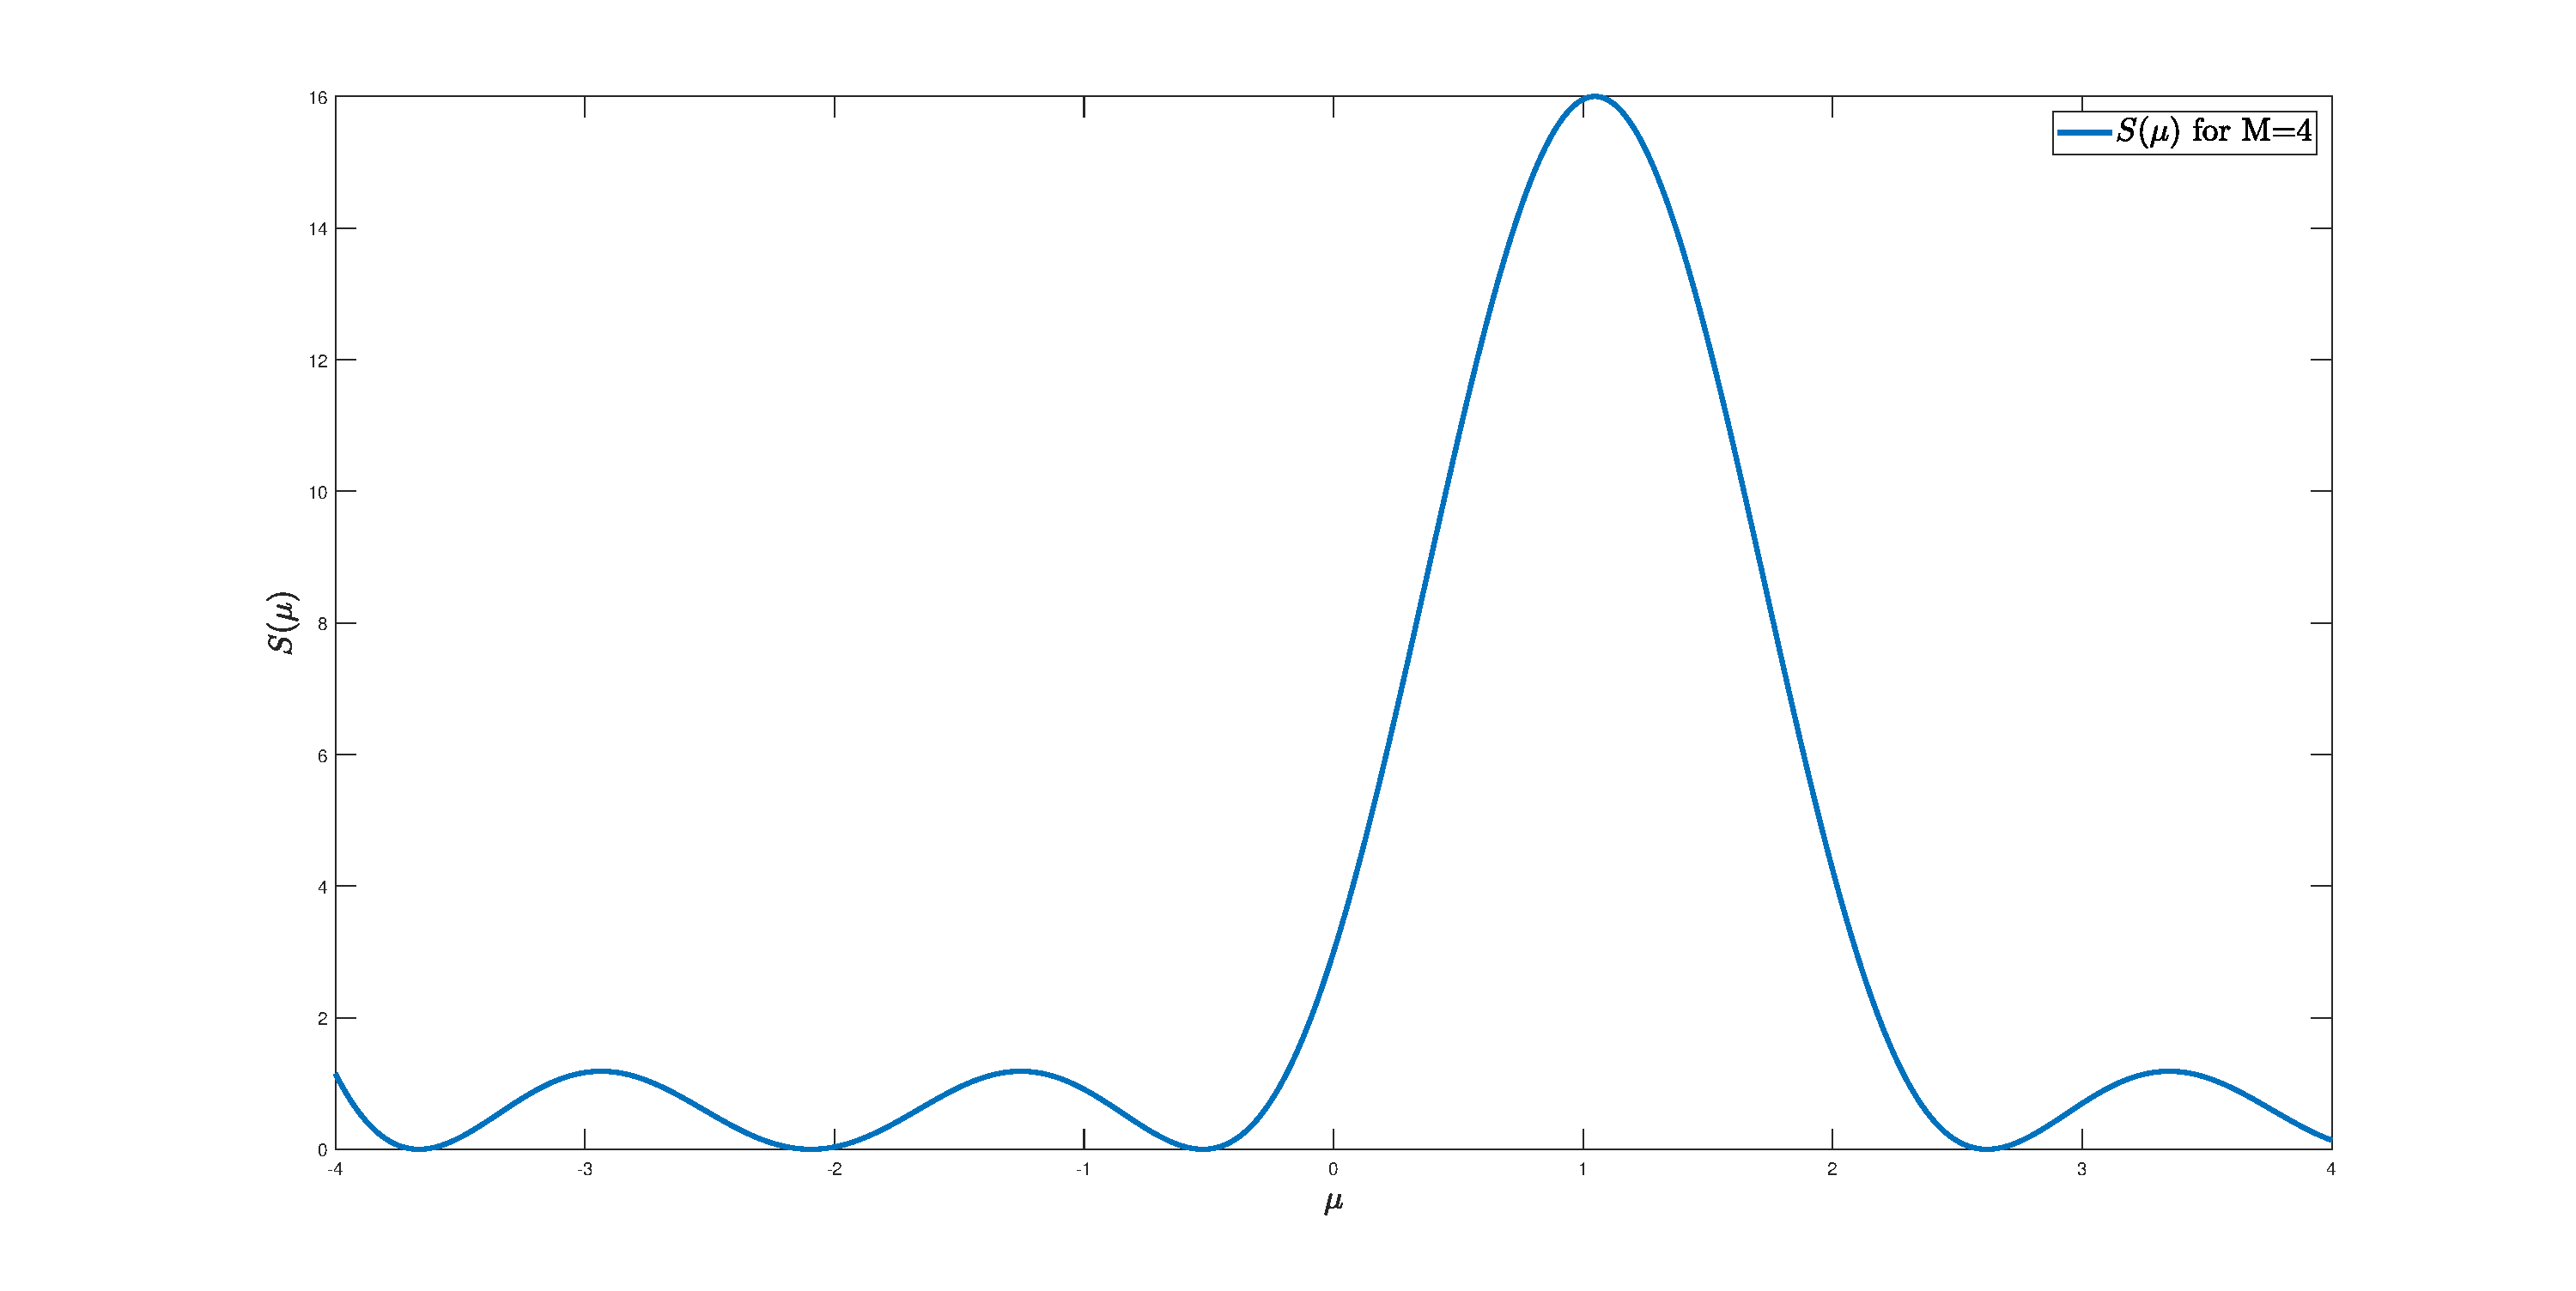
\includegraphics[trim =3cm 1cm 3cm 0cm, clip, width=1.00\textwidth]{graphics/Space_Spectrum_Analyzer_M_4.pdf}
	\caption{Fourier Periodogram for four sensors ($M=4$)}
	\label{fig:Space_Spectrum_Analyzer_M_4}
\end{figure}

\begin{figure}[H]
	\centering
		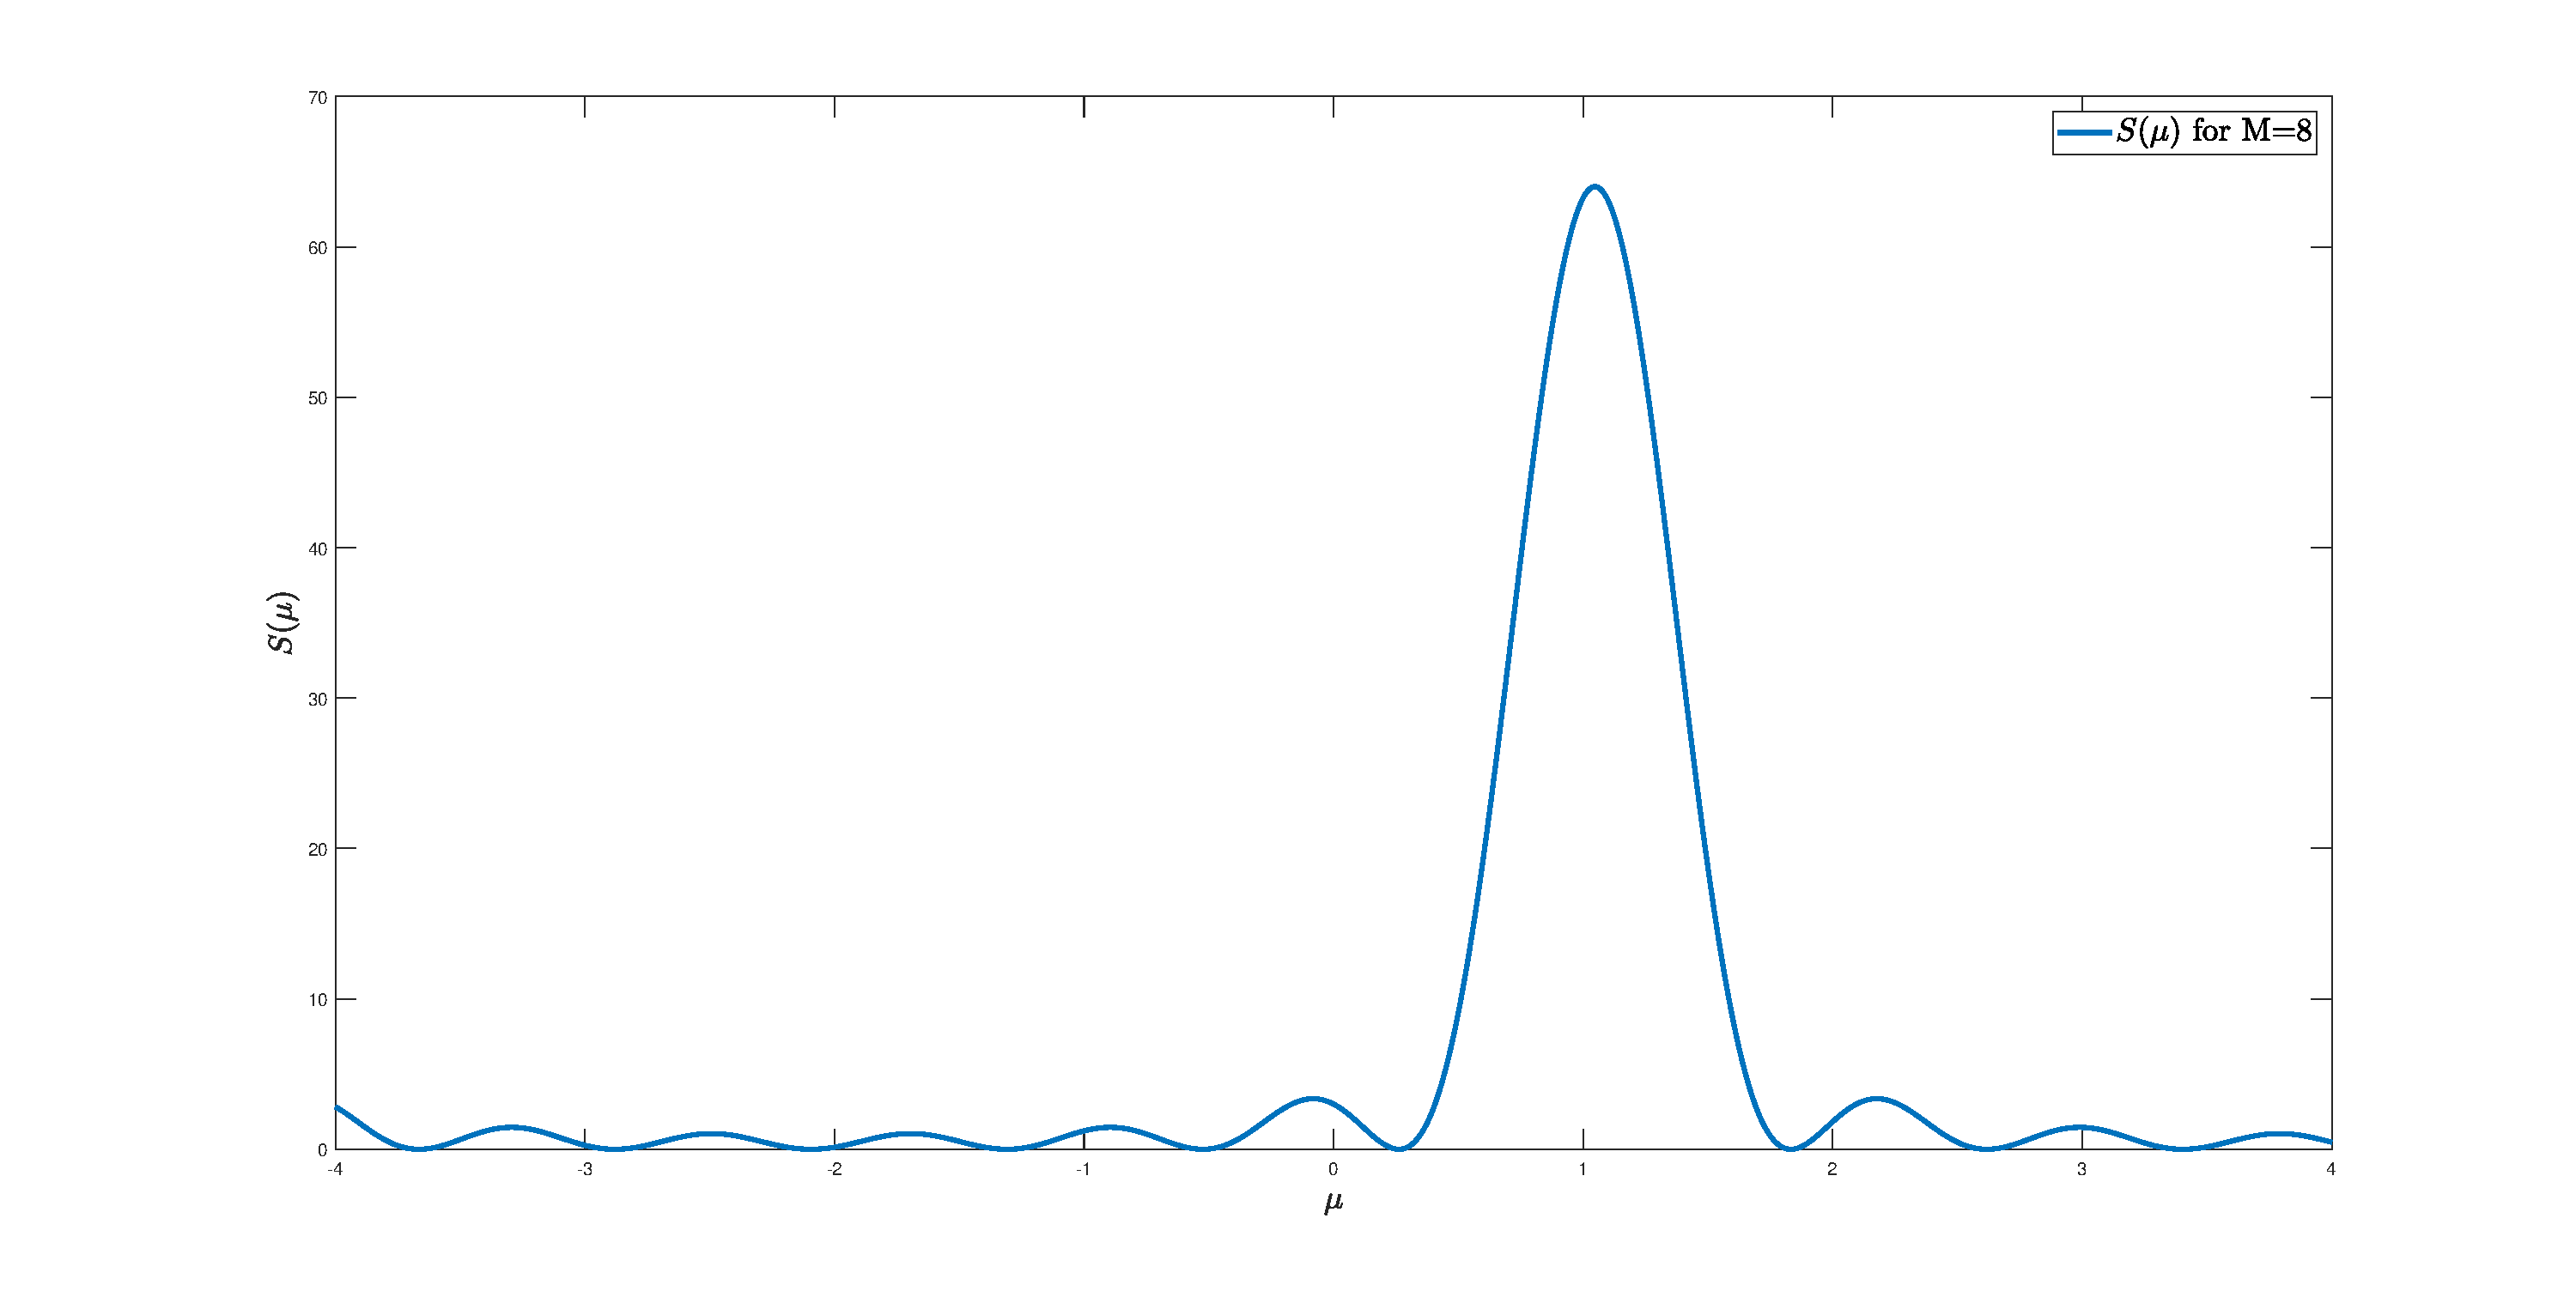
\includegraphics[trim =3cm 1cm 3cm 0cm, clip, width=1.00\textwidth]{graphics/Space_Spectrum_Analyzer_M_8.pdf}
	\caption{Fourier Periodogram for eight sensors ($M=8$)}
	\label{fig:Space_Spectrum_Analyzer_M_8}
\end{figure}

As can be seen from figures \ref{fig:Space_Spectrum_Analyzer_M_4} and \ref{fig:Space_Spectrum_Analyzer_M_8} the resolution is limited. This limit (space between maximum and next zero) is called "Rayleigh-limit" ($\Delta\mu$) and depends on the number of sensors $M$ as follows:\\
$\Delta\mu=\frac{2\pi}{M}$\\
The only way to increase the resolution (decrease "Rayleigh-limit" $\Delta\mu$) is to increase the number of sensors. However this leads to higher costs. Therefore it is not our preferred solution.\\ 
Can we do better?\\ \ \\
\begin{tabular}{ll}
\Ra& Yes, e. g. by using the MVDR (minimum variance distortion-less response) spectrum estimation:\\
 & $S_{MVDR}(\mu)=\frac{1}{\vec{a}^H(\mu)\ma{\hat{R}}_x^{-1}\vec{a}(\mu)}$\\
 & $S_{FPG}(\mu)=\vec{a}^H(\mu)\ma{\hat{R}}_x\vec{a}(\mu)\qquad $ Where FPG stands for Fourier Periodogram (for comparison)\\
\end{tabular}

For \underline{zero noise} the MVDR-spectrum has \underline{no} resolution limitation!\\ 
The MVDR is the same algorithm as the Digital spectrum analyser (\autoref{sssec:dsa}) but with the spatial sampling.
\\ \ \\
Can we do better?\\
\begin{tabular}{ll}
\Ra& Yes, trade-off of SNR with number $N$ of snapshots taken:\\
&$\rightarrow$ \underline{MUSIC}-spectrum:\\
& Resolution depends on $N\cdot SNR$ besides on $M$\\
\end{tabular}
\newpage
\subsection{MUSIC-Algorithm (Multiple Signal Classification)}
\textit{
\begin{center}
"Music was my first love\\
And it will be last."
\end{center}}

Processing the signals received on an array of sensors for the location of the emitter is of great enough interest to have been treated under many special case assumptions. The general problem considers sensors with arbitrary locations and arbitrary directional characteristics (gain/phase/polarization) in a noise interference environment of arbitrary covariance matrix. The \textbf{mu}ltiple \textbf{si}gnal \textbf{c}lassification (MUSIC) algorithm provides asymptotically unbiased estimates of
\begin{enumerate}
	\item number of incident wavefronts present
	\item directions of arrival (DOA) (or emitter locations)
	\item strengths and cross correlations among the incident waveforms
	\item noise/interference strength\cite{Schmidt:MUSIC}
\end{enumerate}

$\vec{x}[n]=\ma{A}\vec{s}[n]+\vec{\nu}[n]$\\
\begin{flalign*}
\ma{A}&=\mat{\vec{a}(\mu_1)& \vec{a}(\mu_2) & \shdots & \vec{a}(\mu_d)}, \qquad \rank\ma{A}=d \pfeil \textrm{steering vectors are LID}&&\\
&=\ma{U}\ma{\Sigma}\ma{V}^H\qquad \text{(SVD)}
\end{flalign*}

$\ma{U}=\mat{\vec{u}_1 & \vec{u}_2 & \shdots & \vec{u}_d & \vec{u}_{d+1} & \vec{u}_{d+2} &\shdots & \vec{u}_M}$\\
We can partition \ma{U} into the two matrices $\ma{U}_1$ and $\ma{U}_2$ ($\ma{U}=\mat{\ma{U}_1 & \ma{U}_2}$) with\\
$\ma{U}_1 = \mat{\vec{u}_1 & \vec{u}_2 & \shdots & \vec{u}_d}$\\
and
$\ma{U}_2 = \mat{\vec{u}_{d+1} & \vec{u}_{d+2} &\shdots & \vec{u}_M}$\\ \\

Recall the properties of matrices from the SVD:\\
$\ma{U}^H_1\ma{U}_1=\ma{I}, \qquad \ma{U}^H_2\ma{U}_2=\ma{I}, \qquad \ma{U}^H_1\ma{U}_2=\ma{0}, \qquad \ma{U}^H_2\ma{U}_1=\ma{0}$\\
$\ma{U}_1\ma{U}^H_1 + \ma{U}_2\ma{U}^H_2 = \ma{I}$\\
$\text{im}\ma{A}= \text{im}\ma{U}_1 \pfeil
\left\lbrace \begin{matrix}
 \forall \mu\in\{\mu_1,\mu_2,\ldots,\mu_d\}:\, \vec{a}(\mu)\in\text{im}\ma{A}\\
 \forall \mu\in\{\mu_1,\mu_2,\ldots,\mu_d\}:\exists\vec{x}:\vec{a}(\mu)=\ma{U}_1\vec{x}
\end{matrix} \right.$\\
Therefore\\
$\ma{U}_2^H\vec{a}(\mu_i)=\underbrace{\ma{U}_2^H\ma{U}_1}{=\ma{0}}\vec{x}=\vec{0}$\\ \ \\

\subsubsection{Ideal MUSIC spectrum}

$S_{\text{MUSIC, IDEAL}}(\mu)=\frac{||\vec{a}(\mu)||_2^2}{||\ma{U}_2^H\vec{a}(\mu)||_2^2}$\\
We assume that $\vec{a}(\mu)\neq0$ holds for any $\mu$.\\ \\

To compute the actual spectrum we divide the $\mu$s into two parts.\\ \\

\textbf{Case 1:}\\
Lets start with $\mu\in\{\mu_1,\ldots,\mu_d\}$:
As we derived above $\ma{U}_2^H\vec{a}(\mu_i)=0$ and therefore it's Euclidean norm is also zero. So we get:\\
$\Rightarrow S_{\text{MUSIC, IDEAL}}(\mu_i)=\infty$\\

\textbf{Case 2:}\\
Assume: $\mat{\vec{a}(\mu_1)& \vec{a}(\mu_2) & \shdots & \vec{a}(\mu_d) & \vec{a}(\mu)}$ are L. I. D. with $\mu\notin\{\mu_1,\ldots,\mu_d\}$.\\
$\vec{a}(\mu)\notin\text{im}\ma{A}=\text{im}\ma{U}_1$\\
$\vec{a}(\mu)\in\text{im}\ma{U}_2$\\
$\vec{a}(\mu)=\ma{U}_2\cdot\vec{y};\qquad \vec{y}\in\mathbb{C}^{(M-d)\times 1};\qquad M-d\geq1$\\
\mybox{
Out of this we get the restriction that the number of sensors must be at least one more than the number of arriving wavefronts:\\
$d\leq M-1$
}
$\ma{U}_2^H\vec{a}(\mu)=\underbrace{\ma{U}_2^H\ma{U}_2}{\ma{I}}\vec{y}=\vec{y}\neq\vec{0}$\\
$\Rightarrow S_{\text{MUSIC, IDEAL}}(\mu)<\infty$ for $\mu\notin\{\mu_1,\ldots,\mu_d\}$\\ \ \\

Summarizing both cases we get:\\
$S_{\text{MUSIC, IDEAL}}(\mu)=\left\lbrace \begin{matrix}\infty,& \text{for} \mu\in\{\mu_1,\ldots,\mu_d\}\\<\infty,&\text{else}\end{matrix} \right.$\\ \ \\

\begin{figure}[H]
	\centering
		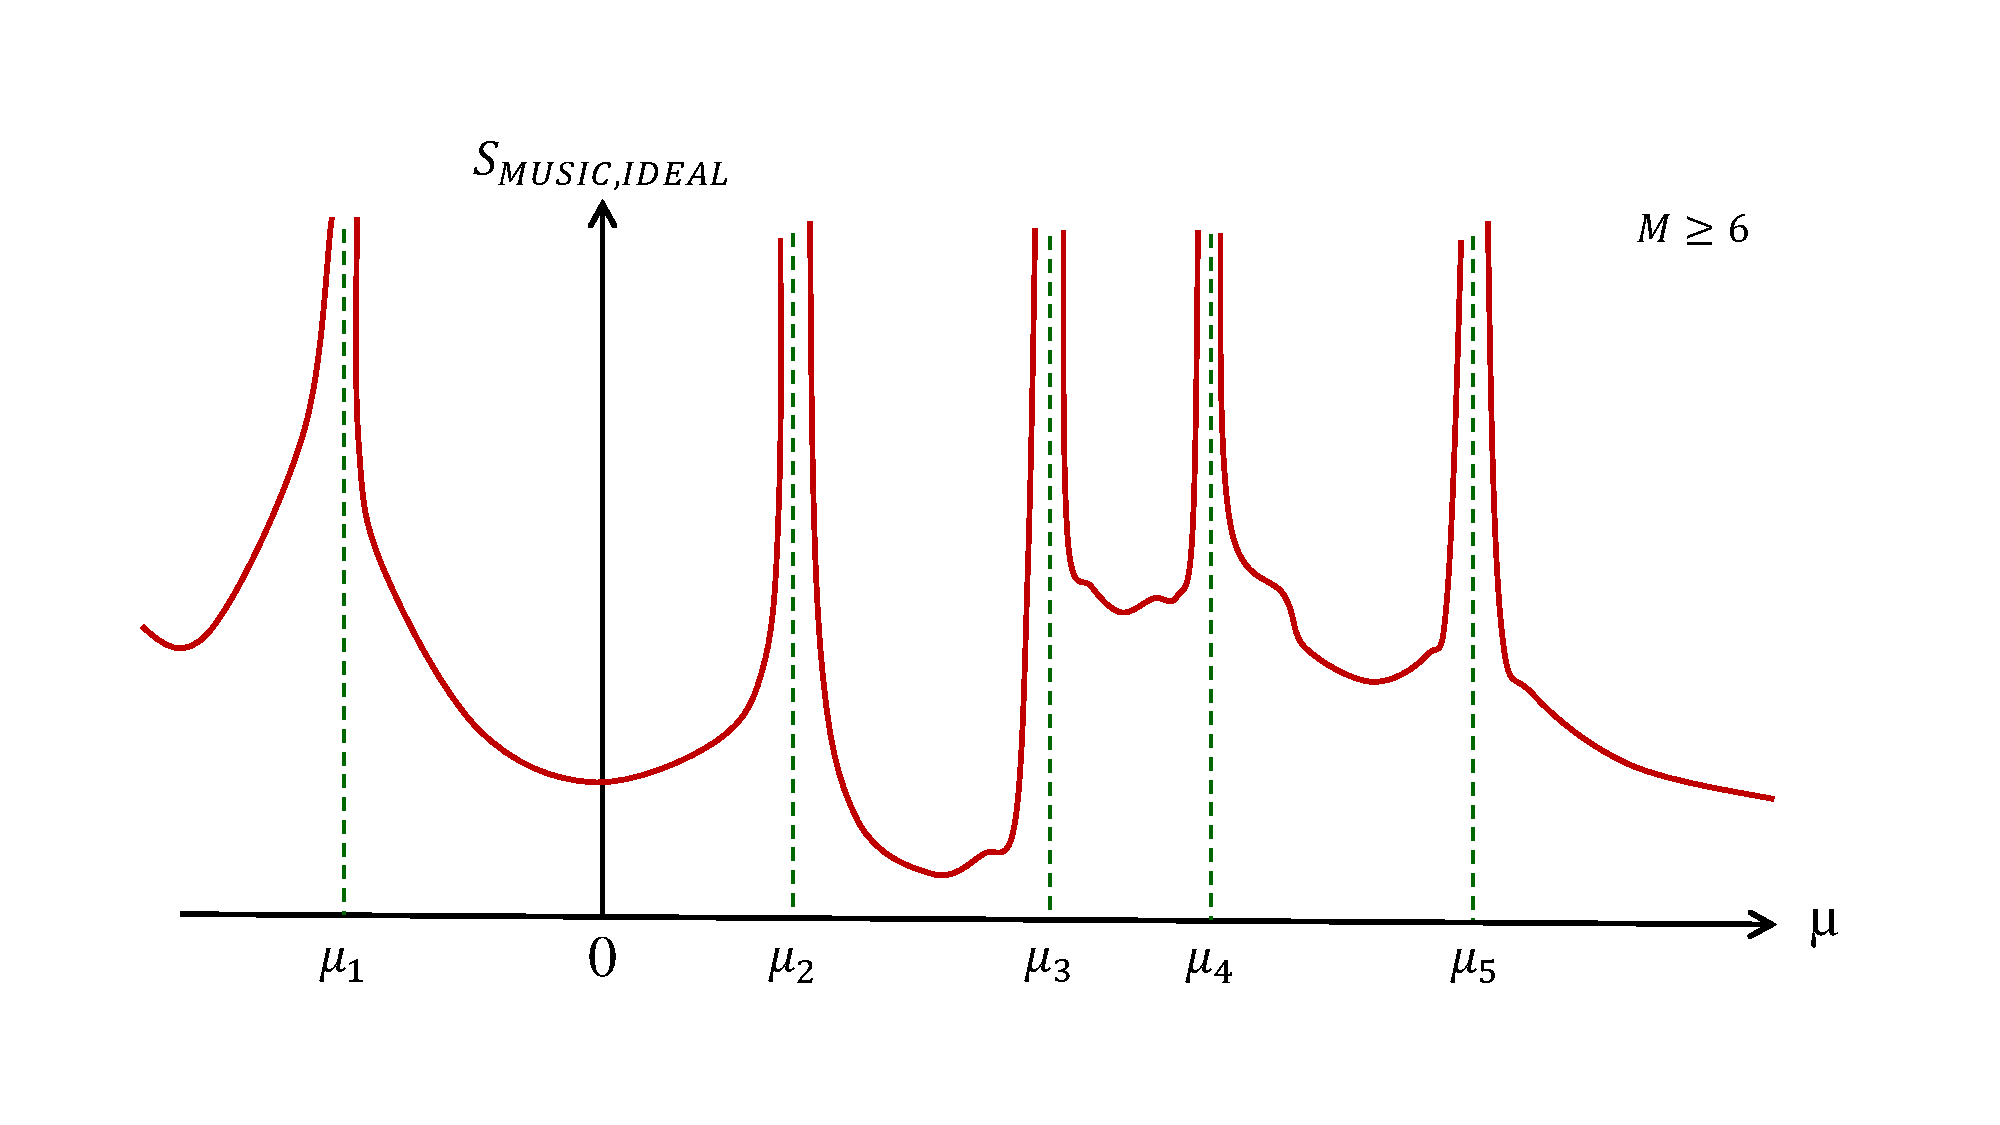
\includegraphics[trim =2cm 2cm 2cm 2cm, clip, width=0.90\textwidth]{graphics/Ideal_MUSIC_spectrum.pdf}
	\caption{Ideal MUSIC spectrum \Ra no resolution limit!}
	\label{fig:Ideal_MUSIC_spectrum}
\end{figure}
As we can see in figure \ref{fig:Ideal_MUSIC_spectrum} there is no resolution limit in the ideal music spectrum. We can be as precise as necessary.

\subsubsection{Problems with the MUSIC spectrum}
However we got 2 problems:
\begin{enumerate}
	\item $\mat{\vec{a}(\mu_1)& \vec{a}(\mu_2) & \shdots & \vec{a}(\mu_d) & \vec{a}(\mu)}$ may L. D.
	\item We don't know $\ma{U}_2$ because \ma{A} is unknown 
\end{enumerate}

\paragraph{Problem 1: Linear dependence of steering vectors}
Let's first look a bit deeper into problem 1:\\
Intuitively it create linear dependent steering vectors (\vec{a}) seems only possible if we place the sensors (antennas) in a well-arranged structure. So we consider an uniform linear array (ULA) that is such a structure.\\
$\vec{a}(\mu_1)=\mat{1\\a\\a^2},\qquad\vec{a}(\mu_2)=\mat{1\\b\\b^2},\vec{a}(\mu)=\mat{1\\c\\c^2}$\\
where $a=e^{\j\mu_1},\quad b=e^{\j\mu_2},\quad c=e^{\j\mu}$ and $a\neq b,\quad a\neq c, b\neq c$\\
$\mat{1&1&1\\a&b&c\\a^2&b^2&c^2}\mat{\alpha\\\beta\\\gamma}=\vec{0}$\\
In order to solve this set of linear equations we use the Gaussian elimination:\\
$\mat{1&1&1\\0&a-b&a-c\\0&a^2-b^2&a^2-c^2}\mat{\alpha\\\beta\\\gamma}=\mat{0\\0\\0}$\\
$\mat{1&1&1\\0&a-b&a-c\\0&0&(c-b)(a-c)}\mat{\alpha\\\beta\\\gamma}=\mat{0\\0\\0}$\\
Since $(c-b)(a-c)\neq 0$ we get:\\
$\gamma=0$\\
The same happens for $\beta$ and $\alpha$:\\
$\underbrace{(a-b)}_{\neq 0} \beta = 0 \Ra \beta=0$\\
$\alpha=0$\\
This means, that even for an ULA we get L. I. D steering vectors if $\Delta<\frac{\lambda}{2}$.\\
It turns out that it is quiet hard to place the sensors such that the steering vectors are L. D.  So in general problem 1 does not affect us in most of the cases.

\paragraph{Problem 2: Determine the steering matrix A}
Recall the singular value decomposition (SVD) of matrix \ma{A}:
$\ma{A}=\ma{U}\ma{\Sigma}\ma{V}^H$\\
$\ma{A}\ma{R}_s\ma{A}^H=\ma{U}\underbrace{\ma{\Sigma}\ma{V}^H\ma{R}_s\ma{V}\ma{\Sigma}^T}_{\ma{\Lambda}}\ma{U}^H=\ma{U}\ma{\Lambda}\ma{U}^H$\\
Where $\ma{\Lambda}$ is the eigenvalue matrix.\\
Now let's assume $\ma{R}_s$ has full rank, which means $\rank\ma{R}_s=d$. Therefore the eigenvalue decomposition (EVD) of $\ma{R}_s$ exists and is given as follows:\\
$\ma{R}_s=\ma{Q}\ma{\Lambda}'\ma{Q}^H;\qquad \ma{\Lambda}'>\vec{0}$ (positive definite)\\
$\ma{R}_s^{\frac{1}{2}}=\ma{Q}\ma{\Lambda}'^{\frac{1}{2}}\ma{Q}^H$\\
Since $\ma{\Lambda}'^{\frac{1}{2}}$ is real valued we can conclude: $\left(\ma{R}^{\frac{1}{2}}\right)^H=\ma{R}^{\frac{1}{2}}$\\
$\ma{A}\ma{R}_s\ma{A}^H=\ma{A}\ma{R}^{\frac{1}{2}}\ma{R}^{\frac{1}{2}}\ma{A}^H=\underbrace{\ma{A}\ma{R}^{\frac{1}{2}}}_{\ma{G}}\underbrace{\left(\ma{R}^{\frac{1}{2}}\right)^H\ma{A}^H}_{\ma{G}^H}=\ma{G}\ma{G}^H$\\
$\Ra \ma{A}\ma{R}_s\ma{A}^H$ turns out to be a Gramian matrix (see section \ref{sec:Gramian_matrix}).\\
\begin{flalign*}
\text{im}\ma{A}\ma{R}_s\ma{A}^H&=\text{im}\ma{G}\ma{G}^H&&\\
&=\text{im}\ma{A}\ma{R}^{\frac{1}{2}}&&\\
&=\text{im}\ma{A}\qquad \text{since } \ma{R}^{\frac{1}{2}} \text{ is invertible}
\end{flalign*}
$\text{im}\ma{A}=\left\lbrace\ma{A}\vec{x}\left.\right|\vec{x}\in\mathbb{C}^{d\times 1}\right\rbrace$\\
$\text{im}\ma{A}\ma{R}^{\frac{1}{2}}=\left\lbrace\ma{A}\underbrace{\ma{R}^{\frac{1}{2}}\vec{y}}_{=\vec{x}}\left.\right|\vec{y}\in\mathbb{C}^{d\times 1}\right\rbrace$\\
Note: $\vec{x}=\ma{R}^{\frac{1}{2}}\vec{y} \Ra \vec{y}=\ma{R}^{-\frac{1}{2}}\vec{x}$\\
$\rank\ma{A}\ma{R}_s\ma{A}^H=\rank\ma{A}=d$\\
$\ma{A}\ma{R}_s\ma{A}^H=\ma{U}\ma{\Lambda}\ma{U}^H=\mat{\ma{U}_1&\ma{U}_2}\mat{\lambda_1& & & & & & \\ &\lambda_2 & & & & &\\ & &\ddots& & & &\\ & & &\lambda_d& & &\\ & & & & 0& &\\ & & & & & \ddots& \\& & & & & &0}\mat{\ma{U}_1^H\\\ma{U}_2^H}$\\
$\vec{x}[n]=\ma{A}\vec{s}[n]+\vec{\nu}[n]$\\
If we assume that noise and signal are uncorrelated (what usually is the case)  we get the following:\\
\mybox{
$E\left[\vec{x}[n]\vec{x}^H[n]\right]=\ma{R}_x=\ma{A}\ma{R}_s\ma{A}^H+\ma{R}_\nu$}\\
Note that $E\left[\vec{x}[n]\vec{x}^H[n]\right]$ can be estimated from array observations.\\
$\ma{\hat{R}}_x=\frac{1}{N}\ma{X}\ma{X}^H$\\
To make things easier we assume the noise to be white which means $\ma{R}_\nu=\sigma_\nu^2\ma{I}$. So we get:\\
\begin{flalign*}
\ma{R}_x&=\underbrace{\ma{A}\ma{R}_s\ma{A}^H}_{\ma{U}\ma{\Lambda}\ma{U}^H}+\sigma_\nu^2\underbrace{\ma{I}}_{\ma{U}\ma{U}^H}&&\\
&=\ma{U}\underbrace{(\ma{\Lambda}+\sigma_\nu^2\ma{I})}_{=\ma{\Lambda}'}\ma{U}^H
\end{flalign*}
\mybox{
$\ma{R}_x=\ma{U}(\ma{\Lambda}+\sigma_\nu^2\ma{I})\ma{U}^H=\ma{U}\ma{\Lambda}'\ma{U}^H$
}

If we sort the eigenvalues such that $\lambda_1\geq\lambda_2\geq\ldots\geq\lambda_d>0$ we get the following eigenvalue matrix $\ma{\Lambda}'$:\\
$\ma{\Lambda}'=\mat{\lambda_1+\sigma_\nu^2& & & & & & \\ &\lambda_2+\sigma_\nu^2 & & & & &\\ & &\ddots& & & &\\ & & &\lambda_d+\sigma_\nu^2& & &\\ & & & & \sigma_\nu^2& &\\ & & & & & \ddots& \\& & & & & &\sigma_\nu^2}$\\

$\lambda_k'=\lambda_k+\sigma_\nu^2$: Eigenvalue of $\ma{R}_x$

\begin{figure}[H]
	\centering
		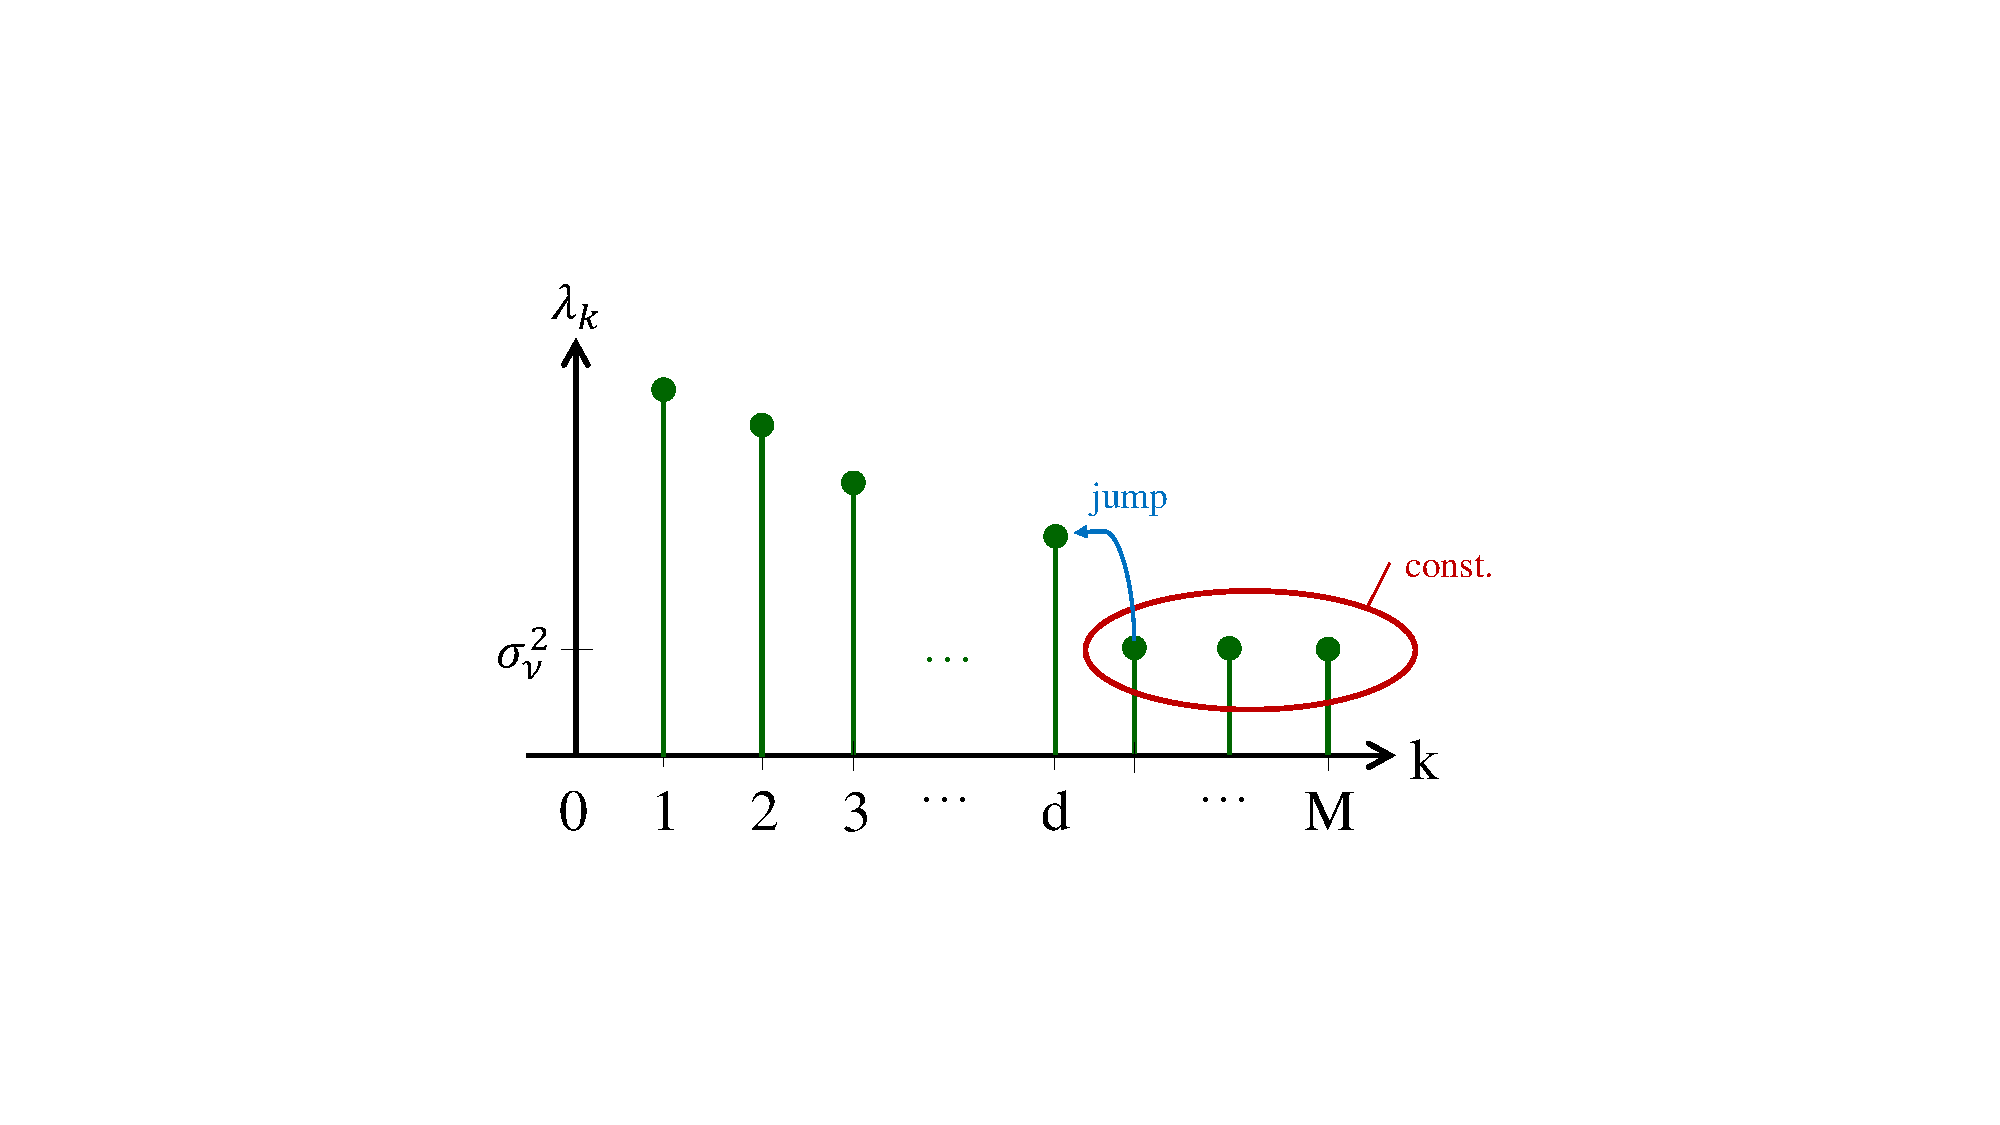
\includegraphics[trim =5cm 5cm 5cm 4cm, clip, width=0.80\textwidth]{graphics/Ideal_MUSIC_eigenvalues.pdf}
	\caption{Ideal (all noise EVs have the same height) eigenvalue spectrum for MUSIC}
	\label{fig:Ideal_MUSIC_eigenvalues}
\end{figure}

From the picture, we get d and can determine $\ma{U}_2$:\\
$\ma{U}_2=\mat{\vec{u}_{d+1}&\vec{u}_{d+1}&\shdots&\vec{u}_{M}}$\\
$\ma{R}_x$ is still unknown but we can take $\ma{\hat{R}}_x$ in its place:\\
$\ma{\hat{R}}_x=\frac{1}{N}\sum\limits_{k=0}^{N-1}\vec{x}[n+k]x^H[n+k]=\frac{1}{N}\ma{X}\ma{X}^H$\\
$\ma{X}=\mat{\vec{x}[n]&\vec{x}[n+1]&\shdots&\vec{x}[n+N-1]}$\\

\begin{figure}[H]
	\centering
		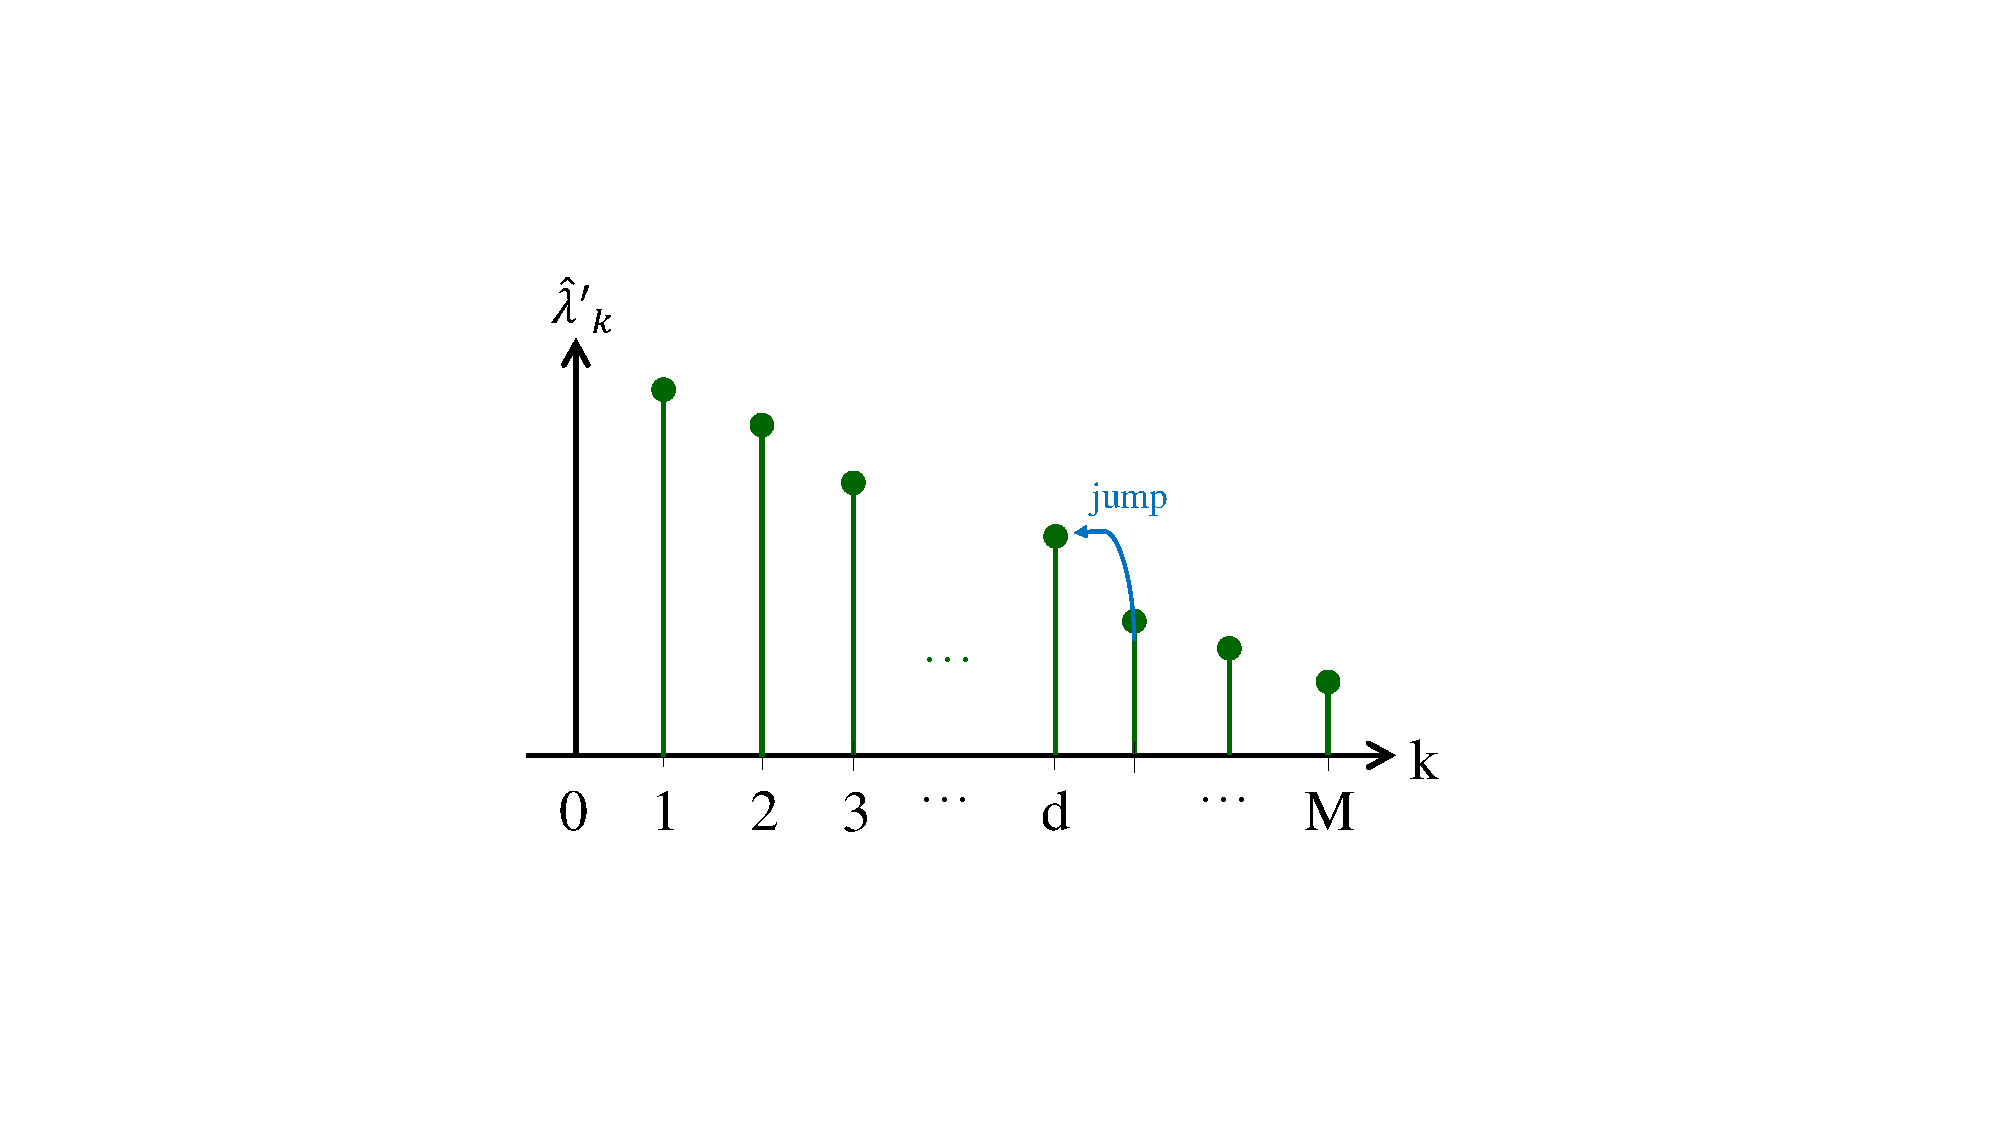
\includegraphics[trim =5cm 5cm 5cm 4cm, clip, width=0.80\textwidth]{graphics/Real_MUSIC_eigenvalues.pdf}
	\caption{Real (noise EVs have NOT the same height) eigenvalue spectrum for MUSIC}
	\label{fig:Real_MUSIC_eigenvalues}
\end{figure}

\newpage
\paragraph{Jump detection}
As can be seen above a jump detection is needed in order to determine the number of arriving wavefronts $d$. This can be done by defining a threshold $q$. If the difference between the m-th eigenvalue and the (m-1)-st is larger than this threshold this is considered as jump and the value for $d$ is found. But now the question is how to set $q$ such that it is neither to small nor to big.\\

\begin{figure}[H]
	\centering
		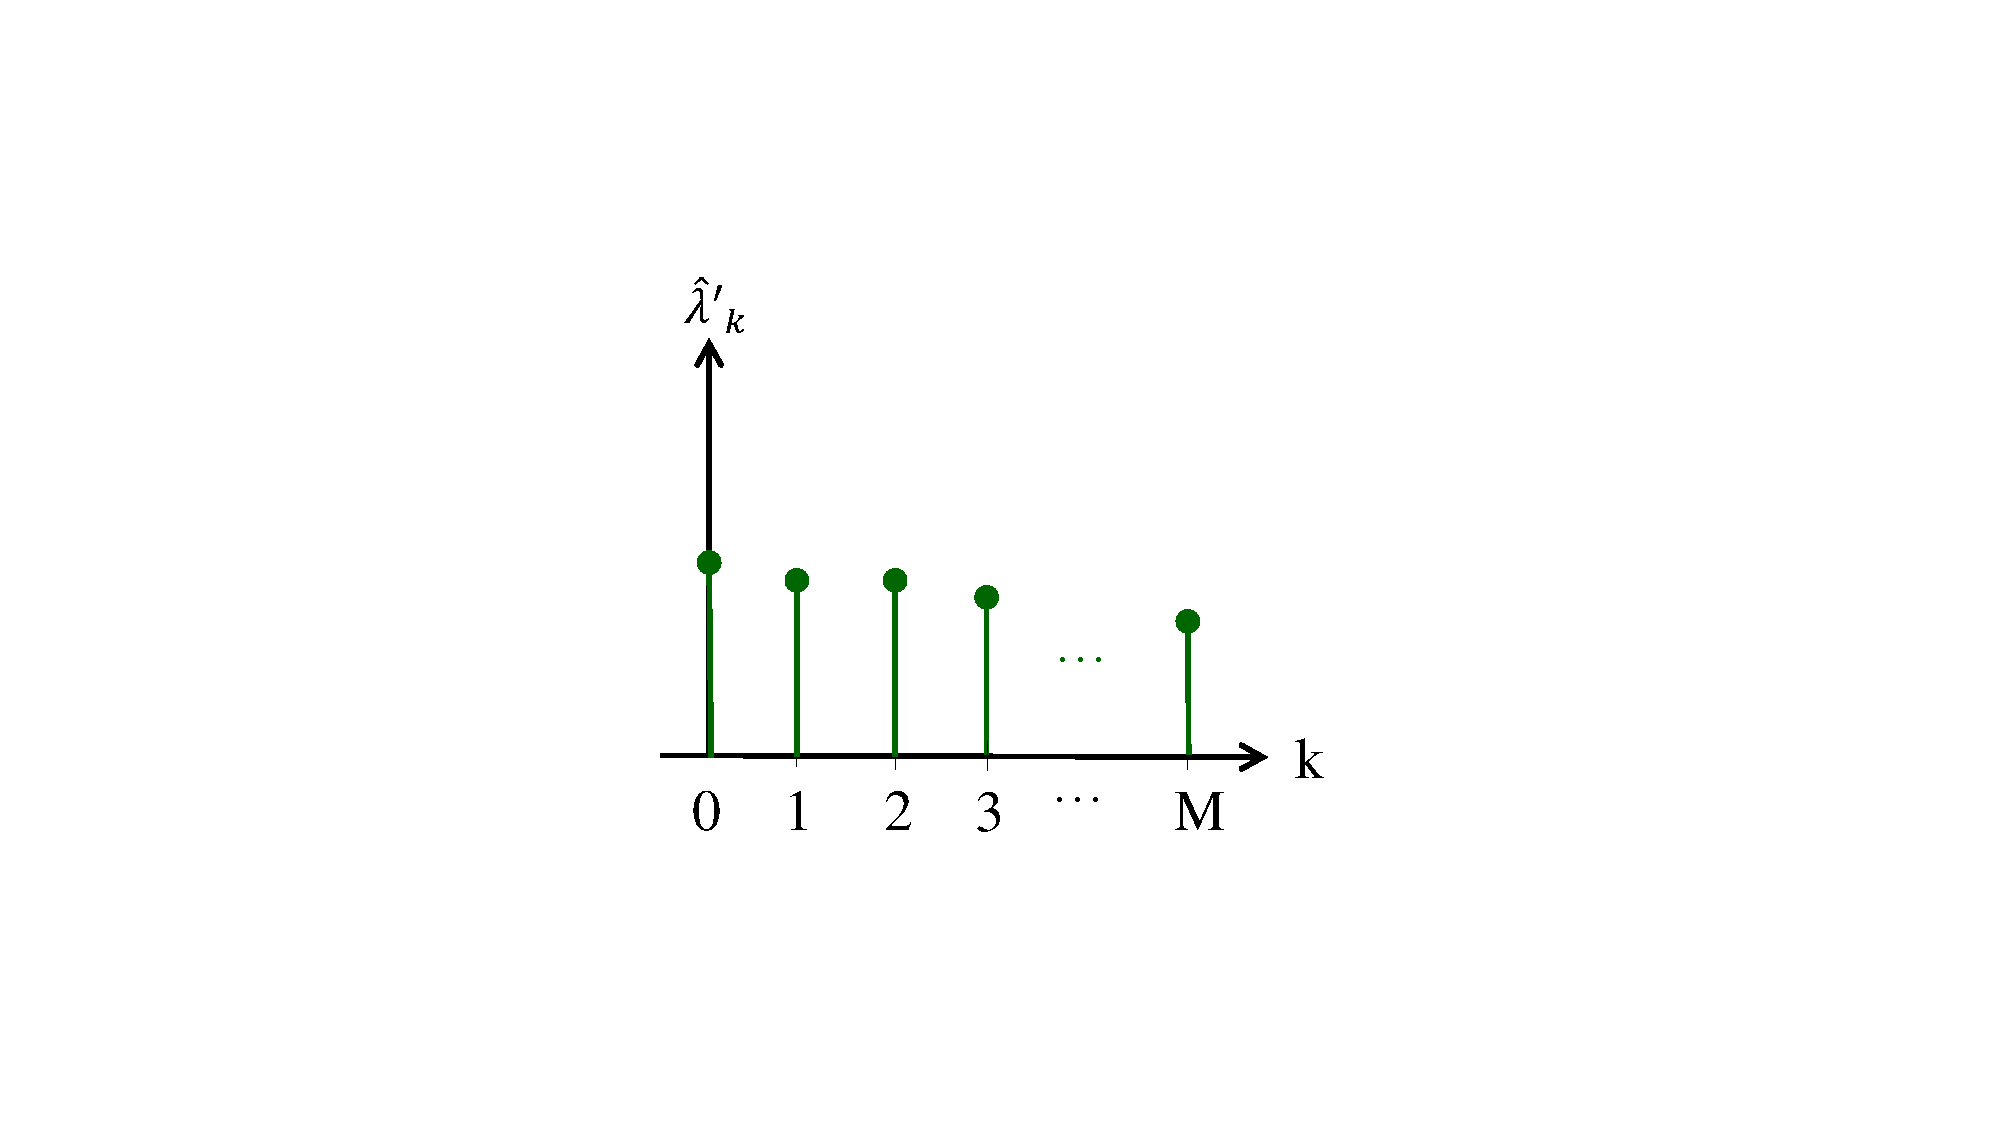
\includegraphics[trim =5cm 5cm 5cm 4cm, clip, width=0.80\textwidth]{graphics/jump_detection_noise.pdf}
	\caption{Noise eigenvalues to determine the minimum jump size $q$}
	\label{fig:jump_detection_noise}
\end{figure}

Let's assume that $d=0$ so we got pure noise. Then we define a probability $p$ of identifying the wrong  $q$:\\

$p=P_r\left[\frac{\hat{\lambda}'_m}{\hat{\lambda}'_{m-1}}>q\right]$\\
After that a Monte-Carlo-Experiment can be run. Out of this experiment jump sizes $q$ can be determined (see table \ref{tab:min_step_size_q}).\\
\begin{table}[H]
\begin{center}
\begin{tabular}{lc|c|c|c}
Sensors&$M$&4&8&8\\
\hline
Snapshots&$N$&100&10&1000\\
\hline
Probability&$p$&0.01&0.01&0.01\\
\hline
Threshold&$q$&\textcolor[rgb]{1,0,0}{1.45}&\textcolor[rgb]{1,0,0}{1.34}&\textcolor[rgb]{1,0,0}{1.09}\\
\end{tabular}
\end{center}
\caption{Results for minimum jump size $q$ (Monte-Carlo-experiment)}
\label{tab:min_step_size_q}
\end{table}

\mybox{
\subsubsection{Summary: MUSIC-Algorithm}
\textbf{Input:} $\ma{X}\in\mathbb{C}^{M\times N};\qquad M=\text{number of sensors},\qquad N=\text{number of snapshots}$\\
\textbf{Output:} $\mu_1,\,\mu_2,\,\ldots,\,\mu_{\hat{d}},\hat{d}$\\
\textbf{Assume white noise!}\\
\begin{enumerate}
	\item $\ma{\hat{R}}_x=\frac{1}{N}\ma{X}\ma{X}^H$ (maximum likelihood estimation for Gauss'ian noise)
	\item EVD: $\ma{\hat{R}}_x=\ma{\hat{U}}\ma{\hat{\Lambda}}'\ma{\hat{U}}^H$
	\item Estimate d: ``Jump detection''
	\item 	Partition $\ma{\hat{U}}$:\\
				$\ma{\hat{U}}=\mat{\vec{\hat{u}}_1&\shdots&\vec{\hat{u}}_{\hat{d}}&\vec{\hat{u}}_{\hat{d}+1}&\shdots&\vec{\hat{u}}_{M}}$; \qquad
				$\ma{\hat{U}}_1=\mat{\vec{\hat{u}}_1&\shdots&\vec{\hat{u}}_{\hat{d}}}$; \qquad
				$\ma{\hat{U}}_2=\mat{\vec{\hat{u}}_{\hat{d}+1}&\shdots&\vec{\hat{u}}_{M}}$\\
				\textcolor[rgb]{1,0,0}{Remember: $\ma{\hat{U}}_2\ma{\hat{U}}_2^H=\ma{I}-\ma{\hat{U}}_1\ma{\hat{U}}_1^H$ may sometimes be easier}
	\item Search for all local maxima of $S_{\text{MUSIC}}(\mu)=\frac{\vec{a}^H(\mu)\vec{a}(\mu)}{\vec{a}^H(\mu)\ma{U}_2\ma{U}_2^H\vec{a}(\mu)}$
	\item \begin{tabular}{ll}
				if number of peaks is & $<\hat{d}: \hat{d}\leftarrow\hat{d}-1$ go back to 4\\
				& $>\hat{d}: \hat{d}\leftarrow\hat{d}+1$ go back to 4
				\end{tabular}
	\item Return the $\mu_i$ at the position of the peaks: $\Rightarrow \ma{\hat{A}}=\mat{\vec{\hat{a}}(\mu_1)&\vec{\hat{a}}(\mu_2)&\shdots&\vec{\hat{a}}(\mu_d)}$
\end{enumerate}}
\ \\
\textbf{How to continue?}\\
 After computing \ma{A} we can proceed in the following way $\ma{R}_s$:\\
$\ma{R}_x=\ma{A}\ma{R}_s\ma{A}^H+\ma{R}_\nu$\\
For white noise: $\ma{R}_\nu=E[|\vec{\nu}|_2^2]\cdot\ma{I}$\\
LS: $\ma{\hat{R}}_s=\ma{\hat{A}}^+\left(\ma{\hat{R}}_x-\ma{\hat{R}}_\nu\right)\left(\ma{\hat{A}}^+\right)^H$\\
$\with \ma{R}_\nu=\sigma_\nu^2\ma{I}$ from $\ma{\Lambda}'$\\
\Ra Now we can apply the MMSE-filter to get the signals $\vec{s}[n]$ out of:\\
$\vec{x}[n]=\ma{A}\vec{s}[n]+\vec{\nu}[n]$

\subsubsection{Preprocessing if noise is not white (colored noise) - Noise Whitening}
So far we assumed that the noise is white. However this may not always be the case. To be still able to compute the signal some kind of preprocessing is needed. Therefore the matrix \ma{T} is used to ``transform'' the input signal such that the MUSIC algorithm works anyway, even if the noise is not white.\\
$\vec{x}[n]=\ma{A}\vec{s}[n]+\ma{\nu}$\\
$\underbrace{\ma{T}\vec{x}[n]}_{=\vec{y}[n]}=\ma{T}\ma{A}\vec{s}[n]+\ma{T}\ma{\nu};\qquad \text{det}\ma{T}\neq 0$ (\ma{T} is invertible)\\
$\ma{T}:=\ma{R}_\nu^{-\frac{1}{2}};\qquad \text{i. e. } \ma{T}\ma{T}=\ma{R}_\nu^{-1}$ (provided that $\ma{R}_\nu^{-1}$ exists)\\
$E\left[\vec{y}[n]\vec{y}^H[n]\right]=\ma{T}\ma{A}\ma{R}_s\ma{A}^H\ma{T}+\ma{I}$\\
$\vec{y}[n]=\mat{\ma{T}\vec{a}(\mu_1)&\ma{T}\vec{a}(\mu_2)&\shdots&\ma{T}\vec{a}(\mu_d)}\vec{s}[n]+\ma{T}\vec{\nu}[n]$\\
Instead of \vec{x} we can feed \vec{y} to the MUSIC algorithm to determine the steering matrix (preprocessing):\\
$\ma{X}\leftarrow\ma{T}\ma{X}$\\
$\vec{a}(\mu)\leftarrow\ma{T}\vec{a}(\mu)$ (run MUSIC)\\ \\
\Ra Remember that the BLUE filter works better as the LS filter if the noise is not white. The Result of the signal with noise whitening with the LS filter is the BLUE filter. \\

BLUE: $\textcolor[rgb]{0,0,1}{\ma{R}_\nu^{-\frac{1}{2}}}\ma{R}_x\textcolor[rgb]{0,0,1}{\ma{R}_\nu^{-\frac{1}{2}}}=\textcolor[rgb]{0,0,1}{\ma{R}_\nu^{-\frac{1}{2}}}\ma{A}\ma{R}_s\ma{A}^H\textcolor[rgb]{0,0,1}{\ma{R}_\nu^{-\frac{1}{2}}}+\underbrace{\textcolor[rgb]{0,0,1}{\ma{R}_\nu^{-\frac{1}{2}}}\ma{R}_\nu\textcolor[rgb]{0,0,1}{\ma{R}_\nu^{-\frac{1}{2}}}}_{=\ma{I}}$\\
$\ma{\hat{R}}_s=\left(\ma{R}_\nu^{-\frac{1}{2}}\ma{A}\right)^+\left(\ma{\hat{R}}_\nu^{-\frac{1}{2}}\ma{\hat{R}}_x\ma{\hat{R}}_\nu^{-\frac{1}{2}}-\ma{I}\right)\left(\ma{R}_\nu^{-\frac{1}{2}}\ma{A}\right)^{+H}$\\ \\
\Ra We see that this is an other way to compute the BLUE.

\subsubsection{Calibration of general sensor positions }
MUSIC is for a ULA, but in general the positions of the sensors are arbitrary. The steering vector can't be determined analytically in general. Therefore the system is measured. 
\begin{figure}[H]
	\centering
		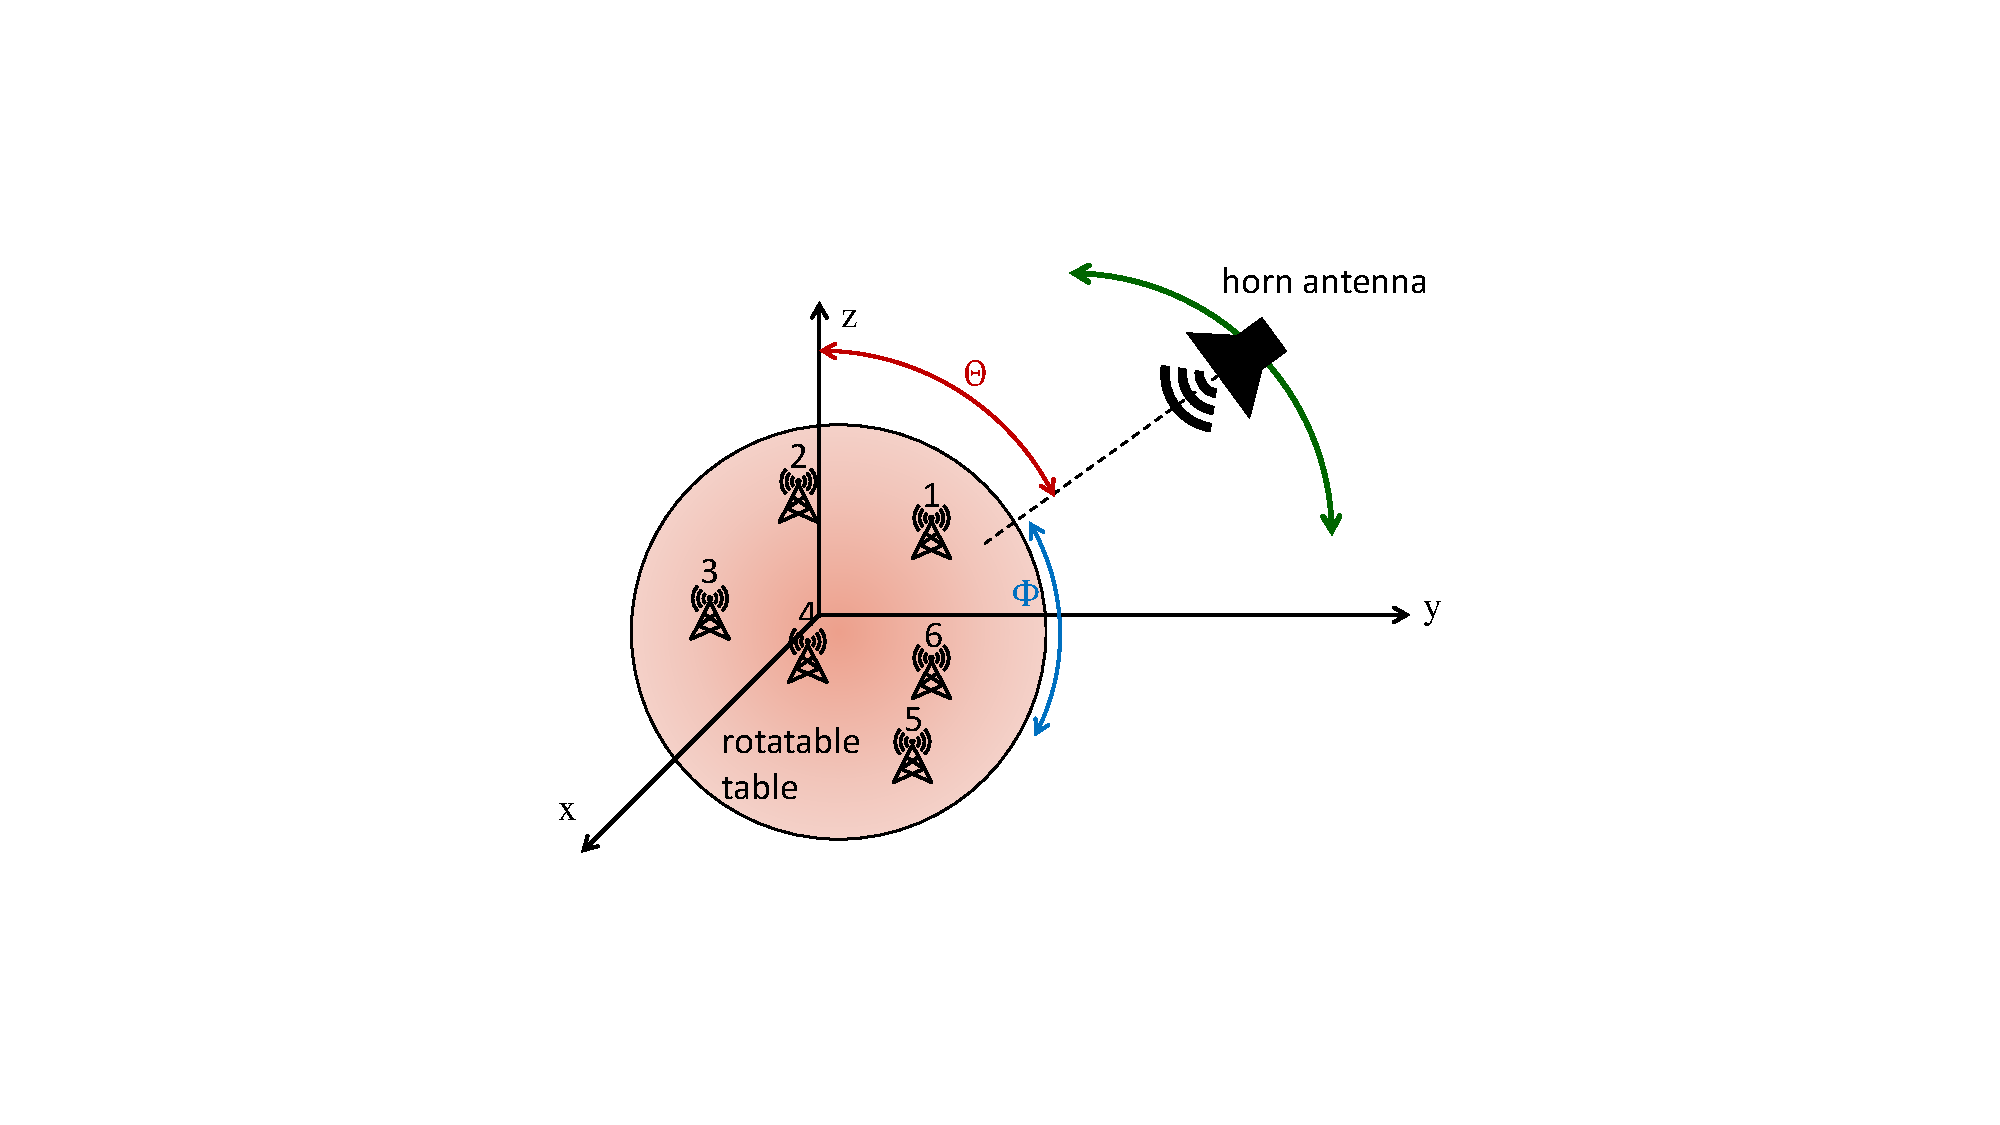
\includegraphics[trim =5cm 3cm 5cm 3cm, clip, width=0.80\textwidth]{graphics/Calibration_scenario.pdf}
	\caption{Calibration of an antenna constellation inside an antenna chamber}
	\label{fig:Calibration_scenario}
\end{figure}

In order to get information about an antenna constellation one usually calibrates the antennas using a reference antenna inside an antenna chamber. Figure \ref{fig:Calibration_scenario} depicts such a calibration figurative. After the measurement an antenna table is obtained. For the example from figure \ref{fig:Calibration_scenario} it could look like:\\
Amplitude Ratio:\\
$\vec{a}(\Theta,\,\Phi)=\mat{1\\\frac{x_2}{x_1}\\\frac{x_3}{x_1}\\\shdots\\\frac{x_6}{x_1}}$

\begin{itemize}
\item get a table of the steering vectors with different $\Theta's$ and $\Phi's$
\item between the values is interpolated (linear, quadratic, spline ...)
\end{itemize}

\subsubsection{ULA with rotation}
\begin{figure}[H]
	\centering
		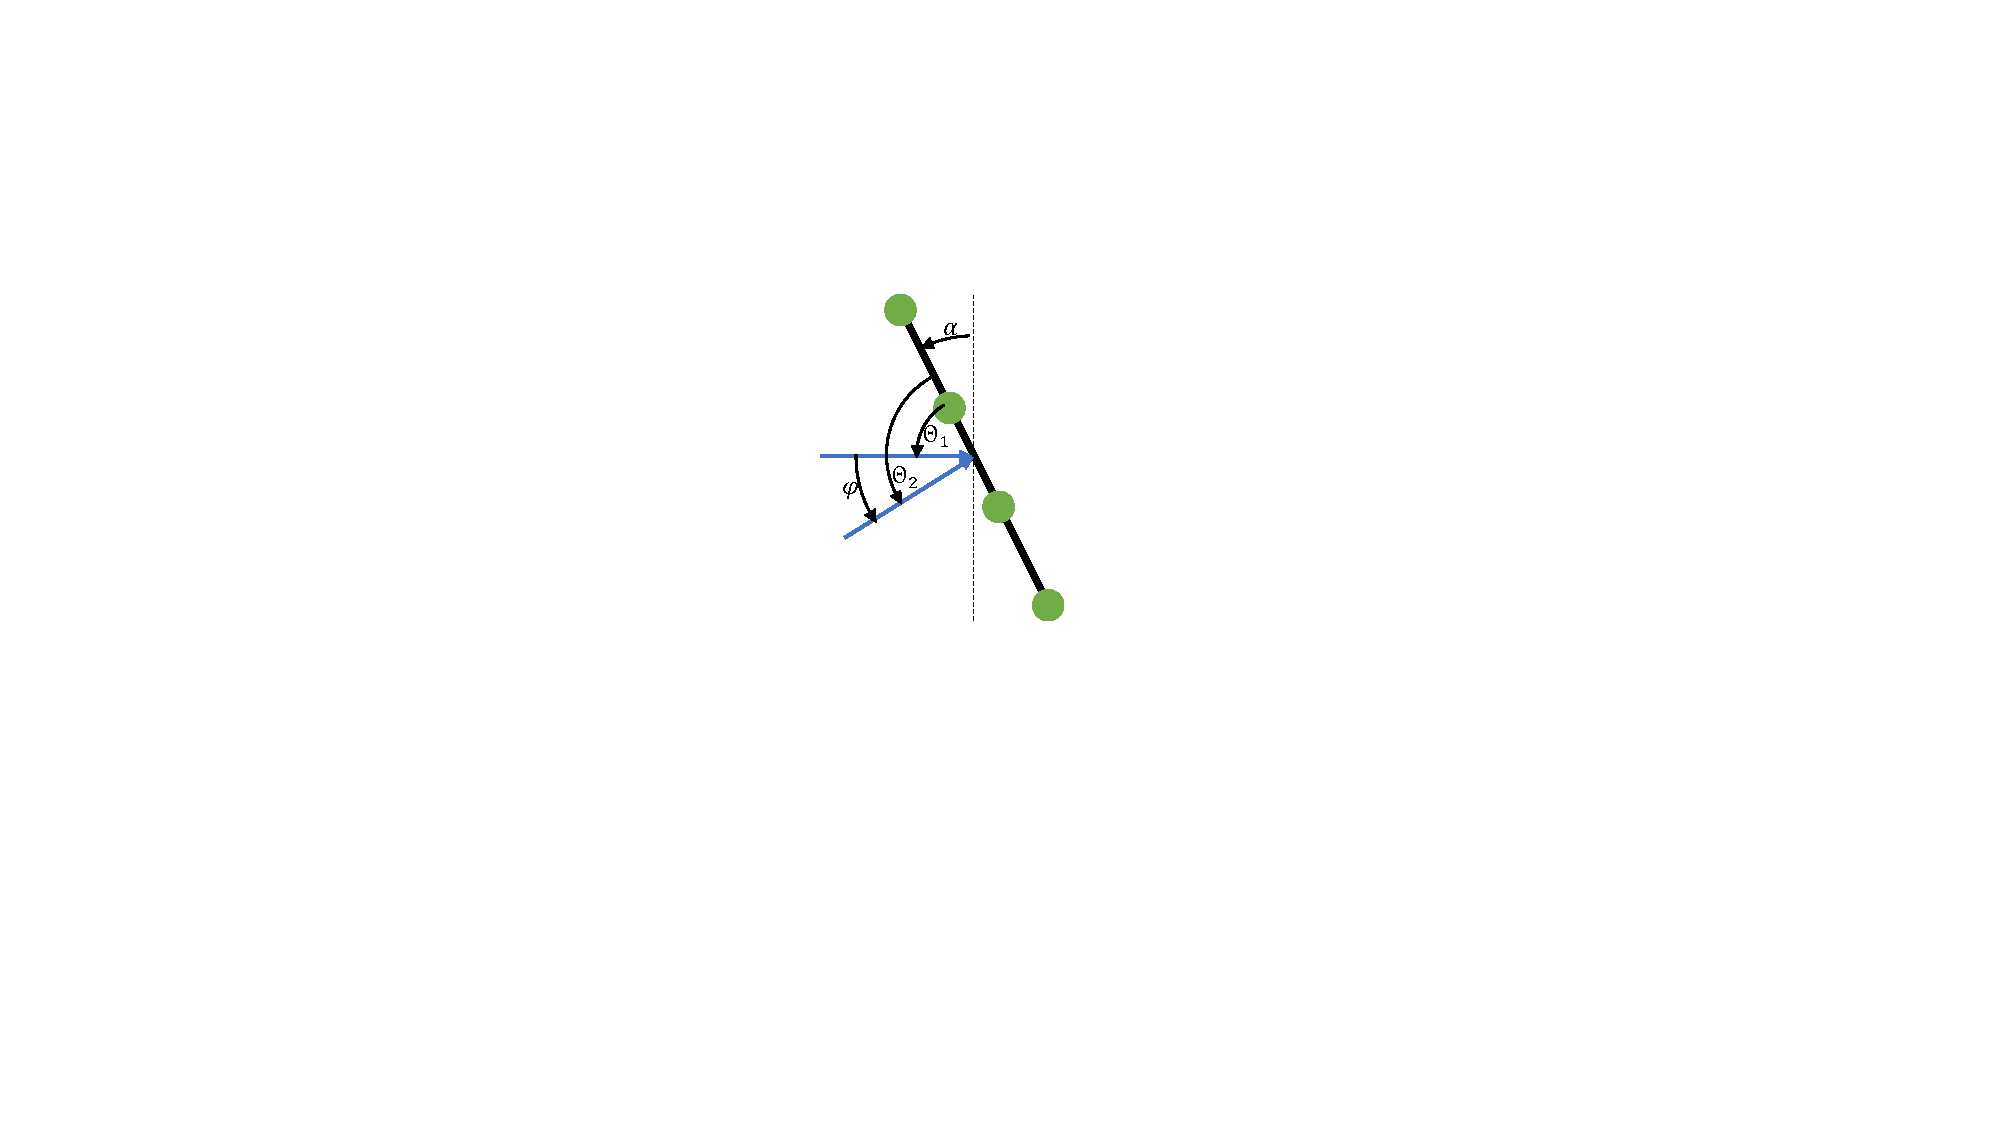
\includegraphics[trim =14cm 8cm 15.5cm 4.7cm, clip, width=0.30\textwidth]{graphics/ULA_angle.pdf}
	\caption{ULA with a rotation angle}
	\label{fig:ULA_angle}
\end{figure}

Incoming signal with two wave fronts:\\
$\vec{x}[n]=\vec{a}(\Theta_1)s_1[n]+\vec{a}(\Theta_2)s_2[n]+\vec{\nu}[n]=\underbrace{\mat{\vec{a}(\Theta_1) &\vec{a}(\Theta_2)}}_{\ma{A}}
\underbrace{\mat{s_1[n]\\s_1[n]}}_{\vec{s}}+\vec{\nu}[n]=\ma{A}\vec{s}+\vec{\nu}[n]$\\
\with $\Theta_1=\frac{\pi}{2}-\alpha$; \qquad $\Theta_2=\Theta_1+\varphi=\frac{\pi}{2}-\alpha+\varphi$ \\

Least Square: $\ma{W}^H=\ma{A}^+$\\
$\vec{\hat{s}}=\ma{A}^+\vec{x}[n]=\ma{A}^+\ma{A}\vec{s}[n]+\ma{A}^+\vec{\nu}$\\
Because $\vec{a}(\Theta_1) ,\vec{a}(\Theta_2)$ ale LID: $\ma{A}^+\ma{A}=\ma{I}$\\
\pfeil $\vec{\hat{s}}=\vec{s}[n]+\underbrace{\ma{A}^+\vec{\nu}}_{\vec{\nu'}}$\\
Observation Noise: $\vec{\nu}$ \pfeil $E[\vec{\nu}\vec{\nu}^H]=\sigma_\nu^2\ma{I}$\\
Estimation Noise: $\vec{\nu}'$\pfeil $E[\abs{\abs{\vec{\nu}}}_2^2]=\sigma_\nu^2\tr\left(\left(\ma{A}^H\ma{A}\right)^{-1}\right)$\\

Signal to Noise Ratio:\\
$SNR=\frac{E[\abs{\abs{\vec{s}}}_2^2]}{\sigma_\nu^2\tr\left(\left(\ma{A}^H\ma{A}\right)^{-1}\right)}$\\

\ \\
Example with 2 antennas and 2 wave fronts:\\
$\ma{A}=\mat{1&1\\e^{-j\pi\cos\Theta_1}&e^{-j\pi\cos\Theta_1}}=
\mat{1&1\\e^{-j\pi\sin\alpha}&e^{-j\pi\sin(\alpha-\varphi)}}$\\
$SNR=\frac{E[\abs{\abs{\vec{s}}}_2^2]}{2\sigma_\nu^2}\cdot\left( 1 -
\underbrace{ \cos\left( \pi \sin \left( \alpha-\varphi\right) -\sin\alpha \right)}_{-1 ... 1} \right)\leq \frac{E[\abs{\abs{\vec{s}}}_2^2]}{\sigma_\nu^2}$\\

Find optimal tilde angle $\alpha$ for the ULA:\\
$\alpha_{opt}=\textrm{arg}\max\limits_{\alpha}SNR = \frac{\varphi}{2}$\\
Best Result: Symmetric situation: \quad $\Theta_1=\frac{\pi}{2}-\frac{\varphi}{2}\qquad\Theta_1=\frac{\pi}{2}+\frac{\varphi}{2} $\\
$SNR_{opt}=\left.  SNR \right|_{\alpha=\frac{\varphi}{2}}=
\frac{E[\abs{\abs{\vec{s}}}_2^2]}{\sigma_\nu^2}\cdot\sin^2\left(\pi \sin \frac{\varphi}{2} \right)$\\

Example: $\varphi=22^\circ \pfeil SNR_{opt}=0.3183 \cdot SNR_{max}$
\newpage
\printbibliography
\end{document}